%%
%% Copyright (c) 2018-2019 Weitian LI <liweitianux@sjtu.edu.cn>
%% Creative Commons BY 4.0
%%

% 模板选项:
%   bachelor|master|doctor  % 必选项
%   fontset=fandol|adobe|windows
%   oneside|twoside
%   openany|openright
%   zihao=-4|5  % 正文字号: 小四(硕士/博士)、五号(学士)
%   english  % 启用英文模版
%   review  % 盲审论文,隐去作者姓名、学号、导师姓名、致谢、发表论文和参与的项目
%   submit  % 定稿提交的论文,插入签名扫描版的原创性声明和授权声明
\documentclass[
  doctor,
  openright,
  twoside,
  %review,
]{sjtuthesis}

\usepackage{xspace}
\usepackage{microtype}
\usepackage{fontawesome5}

\defaultfontfeatures{Mapping=tex-text}
\setmainfont{Source Serif Pro}
\setsansfont{Source Sans Pro}
\setmonofont{Source Code Pro}
\setmathfont{Asana Math}

\setCJKmainfont{Source Han Serif SC}
\setCJKsansfont{FandolKai}
\setCJKmonofont{FandolFang}

\graphicspath{{./}{figures/}{figures/self/}}

% biblatex
% Credit: http://www.khirevich.com/latex/biblatex/
\ExecuteBibliographyOptions{
  backref=true,
  mincitenames=1,
  maxcitenames=2,
}
% print author names as small caps
\renewcommand{\mkbibnamegiven}[1]{\textsc{#1}}
\renewcommand{\mkbibnamefamily}[1]{\textsc{#1}}
\renewcommand{\mkbibnameprefix}[1]{\textsc{#1}}
\renewcommand{\mkbibnamesuffix}[1]{\textsc{#1}}
% period after the authors
\renewcommand{\labelnamepunct}{\addperiod\space}
% discard the period at the very end of a record
\renewcommand{\finentrypunct}{}
% discard the period after the doi link
\renewcommand{\newunitpunct}{\addspace\midsentence}
% use lowercase English for backref
\DefineBibliographyStrings{english}{%
  backrefpage  = {\lowercase{s}ee p.}, % for single page number
  backrefpages = {\lowercase{s}ee pp.} % for multiple page numbers
}
\DeclareDelimFormat{finalnamedelim}{\addspace\&\space}
\DeclareFieldFormat[book]{title}{\textbf{#1}\addperiod\space}
\DeclareFieldFormat[article,inproceedings]{title}{\textit{#1}\addperiod\space}
\DeclareFieldFormat[inproceedings]{booktitle}{\textit{#1}\addperiod\space}
\DeclareFieldFormat[article,inproceedings]{volume}{\textbf{#1}\addcolon\space}
\DeclareFieldFormat{pages}{#1\addperiod\space}
%
\newcommand{\citeay}[1]{\citeauthor{#1} \citeyear{#1} \parencite{#1}}
\newcommand{\citet}[1]{\citeauthor{#1} (\citeyear{#1})\cite{#1}}

% Change 'emph' style to bold face
\let\emph\relax  % there's no \RedeclareTextFontCommand
\DeclareTextFontCommand{\emph}{\boldmath\bfseries}

% Use sans-serif for URLs by '\url'
\urlstyle{sf}

% Continuous footnote numbering
\counterwithout{footnote}{chapter}

% Set labels for hyperref's '\autoref'
% Credit: https://tex.stackexchange.com/a/66150
\def\equationautorefname~#1\null{式~(#1)\null}
\def\chapterautorefname~#1\null{第{#1}章\null}
\def\appendixautorefname{附录}
\def\sectionautorefname{\textsection}
\def\subsectionautorefname{\textsection}
\def\figureautorefname{图}
\def\tableautorefname{表}

% Custom commands
\newcommand{\doi}[1]{%
  \textsc{doi}: \href{https://doi.org/#1}{#1}}
\newcommand{\ads}[1]{%
  \textsc{ads}: \href{http://adsabs.harvard.edu/abs/#1}{#1}}
\newcommand{\arxiv}[1]{%
  arXiv: \href{https://arixv.org/abs/#1}{#1}}
\newcommand{\email}[1]{%
  \href{mailto:#1}{\texttt{#1}}}
%
\newcommand{\Cpi}{\symup{\pi}}  % constant pi
\newcommand{\Ce}{\symup{e}}  % constant e
\newcommand{\Ci}{\symup{i}}  % complex i
\newcommand{\R}[1]{\mathrm{#1}}  % text math alphabets
\newcommand{\B}[1]{\symbf{#1}}  % single-letter bold math
\newcommand{\V}[1]{\symbfit{#1}}  % bold italic
\newcommand{\M}[1]{\symbfsf{#1}}  % bold sans-serif (matrix)
\newcommand{\D}[1]{\R{d}#1}
\newcommand{\diff}[2]{\frac{\D{#1}}{\D{#2}}}
\newcommand{\pdiff}[2]{\frac{\partial #1}{\partial #2}}
%
\newcommand{\lcdm}{ΛCDM\xspace}

% New math operators
\DeclareMathOperator{\erf}{erf}
\DeclareMathOperator{\sinc}{sinc}

% siunitx settings and new units
\sisetup{
  range-phrase=\text{--},
  range-units=single,
  product-units=repeat,
  list-separator={, },
  list-final-separator={, and },
  separate-uncertainty=true,
  detect-all,  % detecting fonts
}
%
\DeclareSIUnit\arcsec{arcsec}
\DeclareSIUnit\arcmin{arcmin}
\DeclareSIUnit\cMpc{cMpc}  % comoving Mpc
\DeclareSIUnit\cGpc{cGpc}  % comoving Gpc
\DeclareSIUnit\deg{deg}
\DeclareSIUnit\dyne{dyn}
\DeclareSIUnit\erg{erg}
\DeclareSIUnit\esu{esu}
\DeclareSIUnit\franklin{Fr}
\DeclareSIUnit\gauss{G}
\DeclareSIUnit\hubble{\ensuremath{\mathit{h}}}
\DeclareSIUnit\jansky{Jy}
\DeclareSIUnit\lightyear{ly}
\DeclareSIUnit\parsec{pc}
\DeclareSIUnit\rayleigh{Rayleigh}
\DeclareSIUnit\solarmass{\ensuremath{\mathrm{M}_{\odot}}}
\DeclareSIUnit\statcoulomb{statC}
\DeclareSIUnit\year{yr}
%
\DeclareSIUnit\kpc{\kilo\parsec}
\DeclareSIUnit\mJy{\milli\jansky}
\DeclareSIUnit\mK{\milli\kelvin}
\DeclareSIUnit\Gpc{\giga\parsec}
\DeclareSIUnit\Gyr{\giga\year}
\DeclareSIUnit\Mpc{\mega\parsec}
\DeclareSIUnit\Myr{\mega\year}
\DeclareSIUnit\uG{\micro\gauss}

\usepackage[en-US]{datetime2}

\usepackage{journalabbrv}

\usepackage{acro}  % acronyms, symbols, glossaries
\acsetup{
  list-heading=chapter,
  extra-style=bracket,
  extra-format={\itshape},
}
%%
%% Copyright (c) 2018-2019 Weitian LI <liweitianux@sjtu.edu.cn>
%% Creative Commons BY 4.0
%%

\DeclareAcronym{bw-synthesized}{
  short = \ensuremath{\theta_s},
  long = 综合波束宽度,
  foreign = synthesized beamwidth,
  sort = theta-s,
  class = symbol,
}

\DeclareAcronym{coef-absorption}{
  short = \ensuremath{\kappa},
  long = 吸收系数,
  foreign = absorption coefficient,
  sort = kappa,
  class = symbol,
}

\DeclareAcronym{coef-emission}{
  short = \ensuremath{j_{\nu}},
  long = 发射系数,
  foreign = emission coefficient,
  sort = j-nu,
  class = symbol,
}

\DeclareAcronym{delay-comp}{
  short = \ensuremath{\tau_0},
  long = 补偿延迟,
  foreign = compensating delay,
  sort = tau-0,
  class = symbol,
}

\DeclareAcronym{delay-geo}{
  short = \ensuremath{\tau_g},
  long = 几何延迟,
  foreign = geometric delay,
  sort = tau-g,
  class = symbol,
}

\DeclareAcronym{delta-crit}{
  short = \ensuremath{\delta_c(z)},
  long = 临界线性过密度,
  foreign = critical linear overdensity,
  class = symbol,
}

\DeclareAcronym{distance-angular}{
  short = \ensuremath{D_{\!A}},
  long = 角直径距离,
  foreign = angular diameter distance,
  sort = D-A,
  class = symbol,
}

\DeclareAcronym{distance-luminosity}{
  short = \ensuremath{D_{\!L}},
  long = 光度距离,
  foreign = luminosity distance,
  sort = D-L,
  class = symbol,
}

\DeclareAcronym{distance-comoving}{
  short = \ensuremath{D_{\!M}},
  long = 横向共动距离,
  foreign = transverse comoving distance,
  sort = D-M,
  class = symbol,
}

\DeclareAcronym{Ez}{
  short = \ensuremath{E(z)},
  long = 红移演化因子,
  class = symbol,
}

\DeclareAcronym{freq}{
  short = \ensuremath{\nu},
  long = 频率,
  sort = nu,
  first-style = short,
  class = symbol,
}

\DeclareAcronym{G}{
  short = \ensuremath{G},
  long = 引力常数,
  class = symbol,
}

\DeclareAcronym{h}{
  short = \si{\hubble},
  long = 无量纲 Hubble 常数,
  class = symbol,
}

\DeclareAcronym{H0}{
  short = \ensuremath{H_0},
  long = 当前的 Hubble 常数,
  sort = H-0,
  class = symbol,
}

\DeclareAcronym{Hz}{
  short = \ensuremath{H(z)},
  long = 红移为 $z$ 时的 Hubble 常数,
  sort = H-z,
  class = symbol,
}

\DeclareAcronym{I-nu}{
  short = \ensuremath{I_{\nu}},
  long = 比强度,
  foreign = specific intensity,
  sort = I-nu,
  class = symbol,
}

\DeclareAcronym{kb}{
  short = \ensuremath{k_B},
  long = Boltzmann 常数,
  sort = k-B,
  class = symbol,
}

\DeclareAcronym{L-bolo}{
  short = \ensuremath{L_{\R{bolo}}},
  long = 热光度,
  foreign = bolometric luminosity,
  class = symbol,
}

\DeclareAcronym{M-vir}{
  short = \ensuremath{M_{\R{vir}}},
  long = 维里质量,
  foreign = virial mass,
  class = symbol,
}

\DeclareAcronym{N-ant}{
  short = \ensuremath{N_{\!A}},
  long = 天线数目,
  class = symbol,
}

\DeclareAcronym{ns}{
  short = \ensuremath{n_s},
  long = 原初扰动的标量谱指数,
  foreign = scalar spectral index,
  class = symbol,
}

\DeclareAcronym{Ob0}{
  short = \ensuremath{\Omega_b},
  long = 当前的宇宙重子物质密度参数,
  sort = Omega-b,
  class = symbol,
}

\DeclareAcronym{Ofz}{
  short = \ensuremath{\Omega_f(z)},
  long = 红移为 $z$ 时的宇宙物质比例,
  sort = Omega-f-z,
  class = symbol,
}

\DeclareAcronym{Om0}{
  short = \ensuremath{\Omega_m},
  long = 当前的宇宙物质(包括重子物质和暗物质)密度参数,
  sort = Omega-m,
  class = symbol,
}

\DeclareAcronym{Ol0}{
  short = \ensuremath{\Omega_{\Lambda}},
  long = 当前的宇宙常数或真空能密度参数,
  sort = Omega-Lambda,
  class = symbol,
}

\DeclareAcronym{optical-depth}{
  short = \ensuremath{\tau},
  long = 光深,
  foreign = optical depth,
  sort = tau,
  class = symbol,
}

\DeclareAcronym{overdensity-vir}{
  short = \ensuremath{\Delta_{\R{vir}}},
  long = 星系团的平均过密度,
  foreign = average overdensity,
  sort = Delta-vir,
  class = symbol,
}

\DeclareAcronym{r-core}{
  short = \ensuremath{r_c},
  long = 核半径,
  foreign = core radius,
  class = symbol,
}

\DeclareAcronym{r-scale}{
  short = \ensuremath{r_s},
  long = 标度半径,
  foreign = scale radius,
  class = symbol,
}

\DeclareAcronym{r-vir}{
  short = \ensuremath{r_{\R{vir}}},
  long = 维里半径,
  foreign = virial radius,
  class = symbol,
}

\DeclareAcronym{redshift}{
  short = \ensuremath{z},
  long = 红移,
  foreign = redshift,
  sort = z,
  first-style = short,
  class = symbol,
}

\DeclareAcronym{rho-crit}{
  short = \ensuremath{\rho_{\R{crit}}},
  long = 宇宙临界密度,
  foreign = critical density,
  class = symbol,
}

\DeclareAcronym{S-bolo}{
  short = \ensuremath{S_{\R{bolo}}},
  long = 热流量,
  foreign = bolometric flux,
  class = symbol,
}

\DeclareAcronym{S-uv}{
  short = \ensuremath{S(u,v)},
  long = 采样函数,
  foreign = sampling function,
  class = symbol,
}

\DeclareAcronym{S-nu}{
  short = \ensuremath{S_{\nu}},
  long = 流量密度,
  foreign = flux density,
  sort = S-nu,
  class = symbol,
}

\DeclareAcronym{sigma8}{
  short = \ensuremath{\sigma_8},
  long = 原初扰动在 \SI{8}{\per\hubble\Mpc} 尺度上的幅度,
  sort = sigma-8,
  class = symbol,
}

\DeclareAcronym{spec-index}{
  short = \ensuremath{\alpha},
  long = 谱指数,
  foreign = spectral index,
  sort = alpha,
  class = symbol,
}

\DeclareAcronym{speed-light}{
  short = \ensuremath{c},
  long = 光速,
  sort = c,
  class = symbol,
}

\DeclareAcronym{speed-sound}{
  short = \ensuremath{c_s},
  long = 声速,
  sort = c-s,
  class = symbol,
}

\DeclareAcronym{T-antenna}{
  short = \ensuremath{T_{\!A}},
  long = 天线温度,
  foreign = antenna temperature,
  class = symbol,
}

\DeclareAcronym{T-brightness}{
  short = \ensuremath{T_b},
  long = 亮温度,
  foreign = brightness temperature,
  class = symbol,
}

\DeclareAcronym{T-excitation}{
  short = \ensuremath{T_{\R{ex}}},
  long = 激发温度,
  foreign = excitation temperature,
  class = symbol,
}

\DeclareAcronym{u-nu}{
  short = \ensuremath{u_{\nu}},
  long = 谱能量密度,
  foreign = spectral energy density,
  sort = u-nu,
  class = symbol,
}

\DeclareAcronym{Vis}{
  short = \ensuremath{\symscr{V}},
  long = 复可见度,
  foreign = complex visibility,
  sort = V,
  class = symbol,
}

\DeclareAcronym{wavelength}{
  short = \ensuremath{\lambda},
  long = 波长,
  sort = lambda,
  first-style = short,
  class = symbol,
}

\endinput

%%
%% Copyright (c) 2019 Weitian LI <liweitianux@sjtu.edu.cn>
%% Creative Commons BY 4.0
%%

\DeclareAcronym{21cma}{
  short = 21CMA,
  long = 21 CentiMeter Array,
  class = acronym,
}

\DeclareAcronym{2d}{
  short = 2D,
  long = 二维,
  foreign = two-dimensional,
  first-style = short,
  class = acronym,
}

\DeclareAcronym{3d}{
  short = 3D,
  long = 三维,
  foreign = three-dimensional,
  first-style = short,
  class = acronym,
}

\DeclareAcronym{agn}{
  short = AGN,
  long = 活动星系核,
  foreign = Active Galactic Nucleus,
  class = acronym,
}

\DeclareAcronym{am}{
  short = AM,
  long = 调幅,
  foreign = Amplitude Modulation,
  class = acronym,
}

\DeclareAcronym{astron}{
  short = ASTRON,
  long = Netherlands Institute for Radio Astronomy,
  first-style = short,
  class = acronym,
}

\DeclareAcronym{aui}{
  short = AUI,
  long = {Associated Universities, Inc.},
  first-style = short,
  class = acronym,
}

\DeclareAcronym{bicep}{
  short = BICEP,
  long = Background Imaging of Cosmic Extragalactic Polarization,
  first-style = short,
  class = acronym,
}

\DeclareAcronym{bighorns}{
  short = BIGHORNS,
  long = Broadband Instrument for Global Hydrogen Reionisation Signal,
  class = acronym,
}

\DeclareAcronym{cc}{
  short = CC,
  long = Creative Commons,
  first-style = short,
  class = acronym,
}

\DeclareAcronym{cdae}{
  short = CDAE,
  long = 卷积去噪自编码器,
  foreign = Convolutional Denoising AutoEncoder,
  class = acronym,
}

\DeclareAcronym{cdm}{
  short = CDM,
  long = 冷暗物质,
  foreign = Cold Dark Matter,
  class = acronym,
}

\DeclareAcronym{cern}{
  short = CERN,
  long = European Organization for Nuclear Research,
  extra = {Conseil européen pour la recherche nucléaire},
  first-style = short,
  class = acronym,
}

\DeclareAcronym{cgs}{
  short = CGS,
  long = Centimeter--Gram--Second,
  first-style = short,
  class = acronym,
}

\DeclareAcronym{cmb}{
  short = CMB,
  long = 宇宙微波背景,
  foreign = Cosmic Microwave Background,
  class = acronym,
}

\DeclareAcronym{cnn}{
  short = CNN,
  long = 卷积神经网络,
  foreign = Convolutional Neural Network,
  class = acronym,
}

\DeclareAcronym{cwt}{
  short = CWT,
  long = 连续小波变换,
  foreign = Continuous Wavelet Transform,
  class = acronym,
}

\DeclareAcronym{dae}{
  short = DAE,
  long = 去噪自编码器,
  foreign = Denoising AutoEncoder,
  class = acronym,
}

\DeclareAcronym{dare}{
  short = DARE,
  long = Dark Ages Radio Explorer,
  first-style = short,
  class = acronym,
}

\DeclareAcronym{dla}{
  short = DLA,
  long = 阻尼 Lyα 系统,
  foreign = Damped Lyman α system,
  class = acronym,
}

\DeclareAcronym{edges}{
  short = EDGES,
  long = Experiment to Detect the Global EoR Signature,
  class = acronym,
}

\DeclareAcronym{eor}{
  short = EoR,
  long = 再电离时期,
  foreign = Epoch of Reionization,
  class = acronym,
}

\DeclareAcronym{fast}{
  short = FAST,
  long = Five-hundred-meter Aperture Spherical radio Telescope,
  class = acronym,
}

\DeclareAcronym{fft}{
  short = FFT,
  long = 快速 Fourier 变换,
  foreign = Fast Fourier Transform,
  class = acronym,
}

\DeclareAcronym{fm}{
  short = FM,
  long = 调频,
  foreign = Frequency Modulation,
  class = acronym,
}

\DeclareAcronym{fr}{
  short = FR,
  long = Fanaroff--Riley,
  class = acronym,
}

\DeclareAcronym{fscn}{
  short = FSCN,
  long = 远旁瓣致淆噪声,
  foreign = Far Side-lobe Confusion Noise,
  class = acronym,
}

\DeclareAcronym{gbt}{
  short = GBT,
  long = Green Bank Telescope,
  class = acronym,
}

\DeclareAcronym{gleam}{
  short = GLEAM,
  long = GaLactic and Extragalactic All-sky MWA,
  class = acronym,
}

\DeclareAcronym{gleam-x}{
  short = GLEAM-X,
  long = GaLactic and Extragalactic All-sky MWA eXtended,
  class = acronym,
}

\DeclareAcronym{gmca}{
  short = GMCA,
  long = 广义形态成分分析,
  foreign = Generalized Morphological Component Analysis,
  class = acronym,
}

\DeclareAcronym{gmrt}{
  short = GMRT,
  long = Giant Metrewave Radio Telescope,
  class = acronym,
}

\DeclareAcronym{gpl}{
  short = GPL,
  long = General Public License,
  first-style = short,
  class = acronym,
}

\DeclareAcronym{gps}{
  short = GPS,
  long = 全球卫星定位系统,
  foreign = Global Positioning System,
  class = acronym,
}

\DeclareAcronym{gpu}{
  short = GPU,
  long = 图形处理器,
  foreign = Graphics Processing Unit,
  class = acronym,
}

\DeclareAcronym{hera}{
  short = HERA,
  long = Hydrogen Epoch of Reionization Array,
  class = acronym,
}

\DeclareAcronym{hpbw}{
  short = HPBW,
  long = 半功率波束宽度,
  foreign = Half Power Beam Width,
  class = acronym,
}

\DeclareAcronym{ica}{
  short = ICA,
  long = 独立成分分析,
  foreign = Independent Component Analysis,
  class = acronym,
}

\DeclareAcronym{icm}{
  short = ICM,
  long = 星系团内介质,
  foreign = IntraCluster Medium,
  class = acronym,
}

\DeclareAcronym{icrar}{
  short = ICRAR,
  long = International Centre for Radio Astronomy Research,
  first-style = short,
  class = acronym,
}

\DeclareAcronym{igm}{
  short = IGM,
  long = 星系际介质,
  foreign = InterGalactic medium,
  class = acronym,
}

\DeclareAcronym{ism}{
  short = ISM,
  long = 星际介质,
  foreign = InterSteller medium,
  class = acronym,
}

\DeclareAcronym{leda}{
  short = LEDA,
  long = Large-aperture Experiment to Detect the Dark Ages,
  class = acronym,
}

\DeclareAcronym{lofar}{
  short = LOFAR,
  long = LOw Frequency ARray,
  class = acronym,
}

\DeclareAcronym{lotss}{
  short = LoTSS,
  long = LOFAR Two-metre Sky Survey,
  class = acronym,
}

\DeclareAcronym{lte}{
  short = LTE,
  long = 局部热力学平衡,
  foreign = Local Thermodynamic Equilibrium,
  class = acronym,
}

\DeclareAcronym{lwa}{
  short = LWA,
  long = Long Wavelength Array,
  class = acronym,
}

\DeclareAcronym{miteor}{
  short = MITEoR,
  long = MIT Epoch of Reionization,
  class = acronym,
}

\DeclareAcronym{mwa}{
  short = MWA,
  long = Murchison Widefield Array,
  class = acronym,
}

\DeclareAcronym{nasa}{
  short = NASA,
  long = National Aeronautics and Space Administration,
  first-style = short,
  class = acronym,
}

\DeclareAcronym{nfw}{
  short = NFW,
  long = Navarro--Frenk--White,
  class = acronym,
}

\DeclareAcronym{nrao}{
  short = NRAO,
  long = National Radio Astronomy Observatory,
  first-style = short,
  class = acronym,
}

\DeclareAcronym{nsf}{
  short = NSF,
  long = National Science Foundation,
  first-style = short,
  class = acronym,
}

\DeclareAcronym{paper}{
  short = PAPER,
  long = Precision Array for Probing the Epoch of Reionization,
  class = acronym,
}

\DeclareAcronym{psf}{
  short = PSF,
  long = 点扩散函数,
  foreign = Point Spread Function,
  class = acronym,
}

\DeclareAcronym{rfi}{
  short = RFI,
  long = 射频干扰,
  foreign = Radio Frequency Interference,
  class = acronym,
}

\DeclareAcronym{saras}{
  short = SARAS,
  long = Shaped Antenna measurement of the background RAdio Spectrum,
  class = acronym,
}

\DeclareAcronym{sci-hi}{
  short = SCI-HI,
  long = {Sonda Cosmológica de las Islas para la Detección de Hidrógeno Neutro},
  class = acronym,
}

\DeclareAcronym{si}{
  short = SI,
  long = International System of Units,
  extra = {Système international d'unités},
  first-style = short,
  class = acronym,
}

\DeclareAcronym{ska}{
  short = SKA,
  long = Square Kilometre Array,
  class = acronym,
}

\DeclareAcronym{te}{
  short = TE,
  long = 热力学平衡,
  foreign = Thermodynamic Equilibrium,
  class = acronym,
}

\DeclareAcronym{vla}{
  short = VLA,
  long = Very Large Array,
  class = acronym,
}

\DeclareAcronym{whim}{
  short = WHIM,
  long = 温热星系际介质,
  foreign = Warm Hot Intergalactic Medium,
  class = acronym,
}

\DeclareAcronym{wsrt}{
  short = WSRT,
  long = Westerbork Synthesis Radio Telescope,
  class = acronym,
}


\endinput

%%
%% Copyright (c) 2018-2019 Weitian LI <liweitianux@sjtu.edu.cn>
%% Creative Commons BY 4.0
%%

\DeclareAcronym{21cmline}{
  short = {21\,cm~谱线},
  long = {21\,cm line},
  extra = of neutral hydrogen,
  sort = 21-li-mi-pu-xian,
  first-style = reversed,
  class = glossary,
}

\DeclareAcronym{21cm-tomography}{
  short = {21\,cm~层析成像},
  long = {21\,cm tomography},
  sort = 21-li-mi-ceng-xi,
  first-style = reversed,
  class = glossary,
}

\DeclareAcronym{ab}{
  short = 天线波束,
  long = antenna beam,
  sort = tian-xian-bo-shu,
  first-style = reversed,
  class = glossary,
}

\DeclareAcronym{aoi}{
  short = 无知时期,
  long = Age of Ignorance,
  sort = wu-zhi-shi-qi,
  first-style = reversed,
  class = glossary,
}

\DeclareAcronym{as}{
  short = 综合孔径,
  long = aperture synthesis,
  sort = zong-he-kong-jing,
  first-style = reversed,
  class = glossary,
}

\DeclareAcronym{baseline}{
  short = 基线,
  long = baseline,
  sort = ji-xian,
  first-style = reversed,
  class = glossary,
}

\DeclareAcronym{bbn}{
  short = 太初核合成,
  long = Big Bang Nucleosynthesis,
  sort = tai-chu-he-he-cheng,
  first-style = reversed,
  class = glossary,
}

\DeclareAcronym{bbt}{
  short = 大爆炸理论,
  long = Big Bang Theory,
  sort = da-bao-zha-li-lun,
  first-style = reversed,
  class = glossary,
}

\DeclareAcronym{beam}{
  short = 波束,
  long = beam,
  sort = bo-shu,
  first-style = reversed,
  class = glossary,
}

\DeclareAcronym{beam-primary}{
  short = 初级波束,
  long = primary beam,
  sort = chu-ji-bo-shu,
  first-style = reversed,
  class = glossary,
}

\DeclareAcronym{beam-station}{
  short = 站点波束,
  long = station beam,
  sort = zhan-dian-bo-shu,
  first-style = reversed,
  class = glossary,
}

\DeclareAcronym{beam-synthesized}{
  short = 综合波束,
  long = synthesized beam,
  sort = zong-he-bo-shu,
  first-style = reversed,
  class = glossary,
}

\DeclareAcronym{bf}{
  short = 波束成形,
  long = beamforming,
  sort = bo-shu-cheng-xing,
  first-style = reversed,
  class = glossary,
}

\DeclareAcronym{blazar}{
  short = 耀变体,
  long = blazar,
  sort = yao-bian-ti,
  first-style = reversed,
  class = glossary,
}

\DeclareAcronym{bw-smear}{
  short = 带宽涂污,
  long = bandwidth smearing,
  sort = dai-kuan-tu-wu,
  first-style = reversed,
  class = glossary,
}

\DeclareAcronym{c-conj}{
  short = 复共轭,
  long = complex conjugate,
  sort = fu-gong-e,
  first-style = reversed,
  class = glossary,
}

\DeclareAcronym{cctor}{
  short = 复相关器,
  long = complex correlator,
  sort = fu-xiang-guan-qi,
  first-style = reversed,
  class = glossary,
}

\DeclareAcronym{cd}{
  short = 宇宙黎明,
  long = Cosmic Dawn,
  sort = yu-zhou-li-ming,
  first-style = reversed,
  class = glossary,
}

\DeclareAcronym{chromatic-effect}{
  short = 色彩效应,
  long = chromatic effect,
  sort = se-cai-xiao-ying,
  first-style = reversed,
  class = glossary,
}

\DeclareAcronym{coll-deexcitation}{
  short = 碰撞退激,
  long = collisional de-excitation,
  sort = peng-zhuang-tui-ji,
  first-style = reversed,
  class = glossary,
}

\DeclareAcronym{coll-excitation}{
  short = 碰撞激发,
  long = collisional excitation,
  sort = peng-zhuang-ji-fa,
  first-style = reversed,
  class = glossary,
}

\DeclareAcronym{column-density}{
  short = 柱密度,
  long = column density,
  sort = zhu-mi-du,
  first-style = reversed,
  class = glossary,
}

\DeclareAcronym{comoving-frame}{
  short = 共动参考系,
  long = comoving frame,
  sort = gong-dong-can-kao-xi,
  first-style = reversed,
  class = glossary,
}

\DeclareAcronym{confusion}{
  short = 混淆,
  long = confusion,
  sort = hun-xiao,
  first-style = reversed,
  class = glossary,
}

\DeclareAcronym{conv-theorem}{
  short = 卷积定理,
  long = convolution theorem,
  sort = juan-ji-ding-li,
  first-style = reversed,
  class = glossary,
}

\DeclareAcronym{ctor}{
  short = 相关器,
  long = correlator,
  sort = xiang-guan-qi,
  first-style = reversed,
  class = glossary,
}

\DeclareAcronym{da}{
  short = 黑暗时期,
  long = Dark Ages,
  sort = hei-an-shi-qi,
  first-style = reversed,
  class = glossary,
}

\DeclareAcronym{delay-center}{
  short = 延迟中心,
  long = delay center,
  sort = yan-chi-zhong-xin,
  first-style = reversed,
  class = glossary,
}

\DeclareAcronym{delay-spec}{
  short = 延迟谱,
  long = delay spectrum,
  sort = yan-chi-pu,
  first-style = reversed,
  class = glossary,
}

\DeclareAcronym{dc}{
  short = 方向余弦,
  long = direction cosine,
  sort = fang-xiang-yu-xian,
  first-style = reversed,
  class = glossary,
}

\DeclareAcronym{deconv}{
  short = 解卷积,
  long = deconvolution,
  sort = jie-juan-ji,
  first-style = reversed,
  class = glossary,
}

\DeclareAcronym{detailed-balance}{
  short = 细致平衡,
  long = detailed balance,
  sort = xi-zhi-ping-heng,
  first-style = reversed,
  class = glossary,
}

\DeclareAcronym{dm}{
  short = 暗物质,
  long = dark matter,
  sort = an-wu-zhi,
  first-style = reversed,
  class = glossary,
}

\DeclareAcronym{dirty-map}{
  short = 脏图,
  long = dirty map,
  sort = zang-tu,
  first-style = reversed,
  class = glossary,
}

\DeclareAcronym{dl}{
  short = 深度学习,
  long = deep learning,
  sort = shen-du-xue-xi,
  first-style = reversed,
  class = glossary,
}

\DeclareAcronym{dod}{
  short = 简并度,
  long = degree of degeneracy,
  sort = jian-bing-du,
  first-style = reversed,
  class = glossary,
}

\DeclareAcronym{em-spontaneous}{
  short = 自发发射,
  long = spontaneous emission,
  sort = zi-fa-fa-she,
  first-style = reversed,
  class = glossary,
}

\DeclareAcronym{em-stimulated}{
  short = 受激发射,
  long = stimulated emission,
  sort = shou-ji-fa-she,
  first-style = reversed,
  class = glossary,
}

\DeclareAcronym{exosphere}{
  short = 散逸层,
  long = exosphere,
  sort = san-yi-ceng,
  first-style = reversed,
  class = glossary,
}

\DeclareAcronym{fg-wedge}{
  short = 前景楔形,
  long = foreground wedge,
  sort = qian-jing-xie-xing,
  first-style = reversed,
  class = glossary,
}

\DeclareAcronym{fgavd}{
  short = 前景回避法,
  long = foreground avoidance,
  sort = qian-jing-hui-bi-fa,
  first-style = reversed,
  class = glossary,
}

\DeclareAcronym{fgrm}{
  short = 前景扣除法,
  long = foreground removal,
  sort = qian-jing-kou-chu-fa,
  first-style = reversed,
  class = glossary,
}

\DeclareAcronym{fringe}{
  short = 条纹,
  long = fringe,
  sort = tiao-wen,
  first-style = reversed,
  class = glossary,
}

\DeclareAcronym{g-units}{
  short = 高斯单位制,
  long = Gaussian units,
  sort = gao-si-dan-wei-zhi,
  first-style = reversed,
  class = glossary,
}

\DeclareAcronym{gain}{
  short = 增益,
  long = gain,
  sort = zeng-yi,
  first-style = reversed,
  class = glossary,
}

\DeclareAcronym{gc}{
  short = 星系团,
  long = galaxy cluster,
  sort = xing-xi-tuan,
  first-style = reversed,
  class = glossary,
}

\DeclareAcronym{gl}{
  short = 引力透镜,
  long = gravitational lensing,
  sort = yin-li-tou-jing,
  first-style = reversed,
  class = glossary,
}

\DeclareAcronym{ground-state}{
  short = 基态,
  long = ground state,
  sort = ji-tai,
  first-style = reversed,
  class = glossary,
}

\DeclareAcronym{hi}{
  short = 中性氢,
  long = neutral hydrogen,
  extra = {\normalfont H\textsc{i}},
  sort = zhong-xing-qing,
  first-style = reversed,
  class = glossary,
}

\DeclareAcronym{hii}{
  short = 电离氢,
  long = ionized hydrogen,
  extra = {\normalfont H\textsc{ii}},
  sort = dian-li-qing,
  first-style = reversed,
  class = glossary,
}

\DeclareAcronym{hotspot}{
  short = 热斑,
  long = hot spot,
  sort = re-ban,
  first-style = reversed,
  class = glossary,
}

\DeclareAcronym{hyperfine-splitting}{
  short = 超精细分裂,
  long = hyperfine splitting,
  sort = chao-jing-xi-fen-lie,
  first-style = reversed,
  class = glossary,
}

\DeclareAcronym{imgcube}{
  short = 图像立方,
  long = image cube,
  sort = tu-xiang-li-fang,
  first-style = reversed,
  class = glossary,
}

\DeclareAcronym{inflation}{
  short = 暴胀,
  long = inflation,
  sort = bao-zhang,
  first-style = reversed,
  class = glossary,
}

\DeclareAcronym{ionosphere}{
  short = 电离层,
  long = ionosphere,
  sort = dian-li-ceng,
  first-style = reversed,
  class = glossary,
}

\DeclareAcronym{jet}{
  short = 喷流,
  long = jet,
  sort = pen-liu,
  first-style = reversed,
  class = glossary,
}

\DeclareAcronym{laser}{
  short = 激光,
  long = laser,
  extra = light amplification by stimulated emission of radiation,
  sort = ji-guang,
  first-style = reversed,
  class = glossary,
}

\DeclareAcronym{line-profile}{
  short = 谱线轮廓,
  long = line profile,
  sort = pu-xian-lun-kuo,
  first-style = reversed,
  class = glossary,
}

\DeclareAcronym{lsf}{
  short = 大尺度纤维状结构,
  long = large-scale filaments,
  sort = da-chi-du-xian-wei-zhuang-jie-gou,
  first-style = reversed,
  class = glossary,
}

\DeclareAcronym{magnetosphere}{
  short = 磁层,
  long = magnetosphere,
  sort = ci-ceng,
  first-style = reversed,
  class = glossary,
}

\DeclareAcronym{mainlobe}{
  short = 主瓣,
  long = main lobe,
  sort = zhu-ban,
  first-style = reversed,
  class = glossary,
}

\DeclareAcronym{maser}{
  short = 脉泽,
  long = maser,
  extra = microwave amplification by stimulated emission of radiation,
  sort = mai-ze,
  first-style = reversed,
  class = glossary,
}

\DeclareAcronym{mcf}{
  short = 互相干函数,
  long = mutual coherence function,
  sort = hu-xiang-gan-han-shu,
  first-style = reversed,
  class = glossary,
}

\DeclareAcronym{mem}{
  short = 最大熵方法,
  long = maximum entropy method,
  sort = zui-da-shang-fang-fa,
  first-style = reversed,
  class = glossary,
}

\DeclareAcronym{mesosphere}{
  short = 中间层,
  long = mesosphere,
  sort = zhong-jian-ceng,
  first-style = reversed,
  class = glossary,
}

\DeclareAcronym{mfp}{
  short = 平均自由程,
  long = mean free path,
  sort = ping-jun-zi-you-cheng,
  first-style = reversed,
  class = glossary,
}

\DeclareAcronym{modemix}{
  short = 模式混合,
  long = mode mixing,
  sort = mo-shi-hun-he,
  first-style = reversed,
  class = glossary,
}

\DeclareAcronym{overdensity}{
  short = 过密度,
  long = overdensity,
  sort = gou-mi-du,
  first-style = reversed,
  class = glossary,
}

\DeclareAcronym{passband}{
  short = 通带,
  long = passband,
  sort = tong-dai,
  first-style = reversed,
  class = glossary,
}

\DeclareAcronym{phase-refpos}{
  short = 相位参考位置,
  long = phase reference position,
  sort = xiang-wei-can-kao-wei-zhi,
  first-style = reversed,
  class = glossary,
}

\DeclareAcronym{phased-array}{
  short = 相控阵,
  long = phased array,
  sort = xiang-kong-zhen,
  first-style = reversed,
  class = glossary,
}

\DeclareAcronym{pl}{
  short = 偏振泄漏,
  long = polarization leakage,
  sort = pian-zhen-xie-lou,
  first-style = reversed,
  class = glossary,
}

\DeclareAcronym{pp}{
  short = 功率方向图,
  long = power pattern,
  sort = gong-lv-fang-xiang-tu,
  first-style = reversed,
  class = glossary,
}

\DeclareAcronym{propagator}{
  short = 传播子,
  long = propagator,
  sort = chuan-bo-zi,
  first-style = reversed,
  class = glossary,
}

\DeclareAcronym{ps}{
  short = 功率谱,
  long = power spectrum,
  sort = gong-lv-pu,
  first-style = reversed,
  class = glossary,
}

\DeclareAcronym{pulsar}{
  short = 脉冲星,
  long = pulsar,
  sort = mai-chong-xing,
  first-style = reversed,
  class = glossary,
}

\DeclareAcronym{quasar}{
  short = 类星体,
  long = quasar,
  extra = quasi-stellar radio source,
  sort = lei-xing-ti,
  first-style = reversed,
  class = glossary,
}

\DeclareAcronym{rad-brem}{
  short = 轫致辐射,
  long = bremsstrahlung,
  sort = ren-zhi-fu-she,
  first-style = reversed,
  class = glossary,
}

\DeclareAcronym{rad-ff}{
  short = 自由--自由辐射,
  long = free--free radiation,
  sort = zi-you-zi-you-fu-she,
  first-style = reversed,
  class = glossary,
}

\DeclareAcronym{rad-syn}{
  short = 同步辐射,
  long = synchrotron radiation,
  sort = tong-bu-fu-she,
  first-style = reversed,
  class = glossary,
}

\DeclareAcronym{radiometer}{
  short = 辐射计,
  long = radiometer,
  sort = fu-she-ji,
  first-style = reversed,
  class = glossary,
}

\DeclareAcronym{recombination}{
  short = 复合,
  long = recombination,
  sort = fu-he,
  first-style = reversed,
  class = glossary,
}

\DeclareAcronym{reionization}{
  short = 再电离,
  long = reionization,
  sort = zai-dian-li,
  first-style = reversed,
  class = glossary,
}

\DeclareAcronym{resonant-scattering}{
  short = 共振散射,
  long = resonant scattering,
  sort = gong-zhen-san-she,
  first-style = reversed,
  class = glossary,
}

\DeclareAcronym{rh}{
  short = 射电晕,
  long = radio halo,
  sort = she-dian-yun,
  first-style = reversed,
  class = glossary,
}

\DeclareAcronym{rmh}{
  short = 迷你射电晕,
  long = radio mini-halo,
  sort = mi-ni-she-dian-yuan,
  first-style = reversed,
  class = glossary,
}

\DeclareAcronym{rms}{
  short = 方均根,
  long = root mean square,
  sort = fang-jun-gen,
  first-style = reversed,
  class = glossary,
}

\DeclareAcronym{rr}{
  short = 射电遗迹,
  long = radio relic,
  sort = she-dian-yi-ji,
  first-style = reversed,
  class = glossary,
}

\DeclareAcronym{rrl}{
  short = 射电复合线,
  long = radio recombination line,
  sort = she-dian-fu-he-xian,
  first-style = reversed,
  class = glossary,
}

\DeclareAcronym{rt}{
  short = 辐射转移,
  long = radiative transfer,
  sort = fu-she-zhuan-yi,
  first-style = reversed,
  class = glossary,
}

\DeclareAcronym{sc}{
  short = 超星系团,
  long = supercluster,
  sort = chao-xing-xi-tuan,
  first-style = reversed,
  class = glossary,
}

\DeclareAcronym{sf}{
  short = 采样函数,
  long = sampling function,
  sort = cai-yang-han-shu,
  first-style = reversed,
  class = glossary,
}

\DeclareAcronym{sft}{
  short = 自旋翻转跃迁,
  long = spin-flip transition,
  sort = zi-xuan-fan-zhuan-yue-qian,
  first-style = reversed,
  class = glossary,
}

\DeclareAcronym{sidelobe}{
  short = 旁瓣,
  long = side lobe,
  sort = pang-ban,
  first-style = reversed,
  class = glossary,
}

\DeclareAcronym{singlet}{
  short = 单态,
  long = singlet,
  sort = dan-yi-tai,
  first-style = reversed,
  class = glossary,
}

\DeclareAcronym{skymap}{
  short = 天图,
  long = sky map,
  sort = tian-tu,
  first-style = reversed,
  class = glossary,
}

\DeclareAcronym{snapshot}{
  short = 快照,
  long = snapshot,
  sort = kuai-zhao,
  first-style = reversed,
  class = glossary,
}

\DeclareAcronym{sn-remnant}{
  short = 超新星遗迹,
  long = supernova remnant,
  sort = chao-xin-xing-yi-ji,
  first-style = reversed,
  class = glossary,
}

\DeclareAcronym{snr}{
  short = 信噪比,
  long = signal-to-noise ratio,
  sort = xin-zao-bi,
  first-style = reversed,
  class = glossary,
}

\DeclareAcronym{spec-line}{
  short = 谱线,
  long = spectral line,
  sort = pu-xian,
  first-style = reversed,
  class = glossary,
}

\DeclareAcronym{spillover}{
  short = 漏失,
  long = spillover,
  sort = lou-shi,
  first-style = reversed,
  class = glossary,
}

\DeclareAcronym{spin}{
  short = 自旋,
  long = spin,
  sort = zi-xuan,
  first-style = reversed,
  class = glossary,
}

\DeclareAcronym{src-extended}{
  short = 展源,
  long = extended source,
  sort = zhan-yuan,
  first-style = reversed,
  class = glossary,
}

\DeclareAcronym{src-point}{
  short = 点源,
  long = point source,
  sort = dian-yuan,
  first-style = reversed,
  class = glossary,
}

\DeclareAcronym{station}{
  short = 站点,
  long = station,
  sort = zhan-dian,
  first-style = reversed,
  class = glossary,
}

\DeclareAcronym{T-color}{
  short = 色温度,
  long = color temperature,
  sort = se-wen-du,
  first-style = reversed,
  class = glossary,
}

\DeclareAcronym{t-int}{
  short = 积分时间,
  long = integration time,
  sort = ji-fen-shi-jian,
  first-style = reversed,
  class = glossary,
}

\DeclareAcronym{t-smear}{
  short = 时间涂污,
  long = time smearing,
  sort = shi-jian-tu-wu,
  first-style = reversed,
  class = glossary,
}

\DeclareAcronym{thermosphere}{
  short = 热层,
  long = thermosphere,
  sort = re-ceng,
  first-style = reversed,
  class = glossary,
}

\DeclareAcronym{timescale}{
  short = 时标,
  long = timescale,
  sort = shi-biao,
  first-style = reversed,
  class = glossary,
}

\DeclareAcronym{triplet}{
  short = 三重态,
  long = triplet,
  sort = san-chong-tai,
  first-style = reversed,
  class = glossary,
}

\DeclareAcronym{troposphere}{
  short = 对流层,
  long = troposphere,
  sort = dui-liu-ceng,
  first-style = reversed,
  class = glossary,
}

\DeclareAcronym{v-peculiar}{
  short = 本动速度,
  long = peculiar velocity,
  sort = ben-dong-su-du,
  first-style = reversed,
  class = glossary,
}

\DeclareAcronym{v-proper}{
  short = 自行速度,
  long = proper velocity,
  sort = zi-xing-su-du,
  first-style = reversed,
  class = glossary,
}

\DeclareAcronym{vis}{
  short = 可见度,
  long = visibility,
  sort = ke-jian-du,
  first-style = reversed,
  class = glossary,
}

\DeclareAcronym{w-proj}{
  short = {$w$ 投影},
  long = $w$-projection,
  sort = w-tou-ying,
  first-style = reversed,
  class = glossary,
}

\DeclareAcronym{w-stack}{
  short = {$w$ 堆叠},
  long = $w$-stacking,
  sort = w-dui-die,
  first-style = reversed,
  class = glossary,
}

\DeclareAcronym{wavenumber}{
  short = 波数,
  long = wavenumber,
  sort = bo-shu,
  first-style = reversed,
  class = glossary,
}

\DeclareAcronym{wim}{
  short = 温电离介质,
  long = warm ionized medium,
  sort = wen-dian-li-jie-zhi,
  first-style = reversed,
  class = glossary,
}


\endinput


\AtBeginBibliography{
  \linespread{1.1}
  \small
}
\addbibresource{references.bib}


%=====================================================================

\DTMsavenow{defensedate}
%\DTMsavedate{defensedate}{2019-06-03}  % TODO

% 不得超过 36 字
\title{%
  SKA EoR 探测实验的射电晕前景建模以及\texorpdfstring{\\}{ }%
  EoR 信号分离算法的研究%
}
\keywords{% <=5 个
  低频射电天文,
  再电离时期,
  射电晕,
  微弱信号分离,
  深度学习
}
\author{李维天}
\studentnumber{0130729026}
\advisor{徐海光~教授}
\school{上海交通大学}
\institute{物理与天文学院}
\major{物理学}
\defensedate{%
  \DTMfetchyear{defensedate} 年
  \DTMfetchmonth{defensedate} 月
  \DTMfetchday{defensedate} 日}

\englishtitle{%
  A Study of Foreground Modeling of Radio Halos and \\
  EoR Signal Separation Method for the \\
  SKA EoR Experiment
}
\englishkeywords{%
  low-frequency radio astronomy,
  epoch of reionization,
  radio halos,
  weak signal separation,
  deep learning
}
\englishauthor{\textbf{Weitian Li}}
\englishadvisor{Prof.~\textbf{Haiguang Xu}}
\englishinstitute{School of Physics and Astronomy}
\englishschool{Shanghai Jiao Tong University}
\englishlocation{Shanghai, China}
\englishmajor{Physics}
\englishdate{\DTMusedate{defensedate}}

%---------------------------------------------------------------------
% Copyright @ last page
%
% Date format: yyyy.mm.dd
\newcommand*{\twodigits}[1]{\ifnum#1<10 0\fi\the#1}
\renewcommand*{\today}{%
  \leavevmode\hbox{\the\year.\twodigits\month.\twodigits\day}%
}
\newcommand*{\ccLabel}[2]{%
  \href{https://creativecommons.org/licenses/#1/#2/}{%
    \color{gray}\faCreativeCommons{}~\uppercase{#1}~#2}%
}
\newcommand*{\githubLabel}[2]{%
  \href{http://github.com/#1/#2}{%
    \color{gray}\faGithub{}~#1/#2}%
}
%
\fancypagestyle{lastpage}{
  \fancyhf{}
  \renewcommand{\headrulewidth}{0pt}
  \fancyfoot[L]{\color{gray}\footnotesize%
    \faCopyright{} 2018--2019, Weitian Li \& Haiguang Xu \hspace{0.5em}
    \ccLabel{by}{4.0} \hspace{0.5em}
    \githubLabel{liweitianux}{phd-thesis} \hspace{0.5em}
    \faEdit{} \today
  }
}
\AtEndDocument{%
  \label{doc:lastpage}
  %\ifodd\pageref{doc:lastpage}
    \newpage\mbox{}
    \thispagestyle{lastpage}
  %\fi
}


%=====================================================================
\begin{document}

\maketitle

\makeatletter
\ifsjtu@submit\relax
  \includepdf{scans/originality.pdf}
  \pdfbookmark[0]{\sjtu@label@originality}{originality}
  \cleardoublepage
  \includepdf{scans/authorization.pdf}
  \pdfbookmark[0]{\sjtu@label@authorization}{authorization}
  \cleardoublepage
\else
  \makeDeclareOriginality
  \makeDeclareAuthorization
\fi
\makeatother

%---------------------------------------------------------------------
\frontmatter

%%
%% Copyright (c) 2018-2019 Weitian LI <liweitianux@sjtu.edu.cn>
%% Creative Commons BY 4.0
%%

% 中文摘要,约 1000 字
\begin{abstract}

\acf*{eor}是宇宙演化早期尚不为人所透彻了解的一个重要时期,
从宇宙大爆炸之后约 3 亿年延续到约 10 亿年,对应的红移范围约为 6--15。
第一代恒星和星系在这个时期刚形成不久,
产生紫外和软 X 射线辐射使中性重子物质逐渐被再次电离。
研究 EoR 对于理解第一代天体和宇宙早期结构的形成具有重要意义,
是建立完整的宇宙演化图景的关键之一。
在低频射电波段 ($\sim$\,\SIrange{50}{200}{\MHz}) 探测源自 EoR 的
中性氢 \acs*{21cmline}是目前已提出的研究该时期的最直接和有效的办法。
然而,由于 EoR 信号非常微弱,且淹没在比它强约 4--5 个数量级的前景干扰之中,
因此在研究 EoR 时必须深刻理解各个前景干扰成分的性质,
研发具有针对性的\acs*{fg-rm}和 EoR 信号分离算法。

在多种 EoR 前景干扰成分中,
银河系\acs*{rad-syn}和\acs*{rad-ff}、河外点源等几种主要成分,
已被较广泛地研究过,它们的低频辐射特征以及对 EoR 探测的干扰行为已经基本被弄清楚。
另一方面,星系团射电晕作为一类较常见的河外射电展源,
也将对 EoR 信号探测产生一定程度的影响。
在以往的前景研究中,只有很少几项工作比较简单地触及了射电晕的低频射电辐射。
这些工作对射电晕图像和频谱的建模过于简化,
而且未进一步分析射电晕辐射对 EoR 信号探测的具体影响。
因此,针对 EoR 探测实验的前景干扰和信号分离难题,本文分两个方面开展研究:
首先是对射电晕的低频射电辐射特征进行更完善、更物理的建模,构建更逼真的前景模型,
并在考虑 SKA1-Low 阵列仪器效应的前提下评估射电晕辐射对 EoR 信号探测的影响;
其次是利用改进的前景模型,基于深度学习研发微弱信号分离算法,
用于分离 EoR 信号和前景干扰。

基于 \acl*{PS} 理论和\acs*{turbreacc-model},
实现了针对射电晕形成和演化过程的完整建模,并据此生成了射电晕的模拟天图,
再利用目前最新的 SKA1-Low 阵列布局模拟了包含仪器效应的 SKA1-Low 射电晕图像。
通过在 \numrange{120}{128}、\numrange{154}{162}
和 \numrange{192}{200} \si{\MHz} 三个频带内比较射电晕和 EoR 信号的一维功率谱,
发现在 $\SI{0.1}{\per\Mpc} < k < \SI{2}{\per\Mpc}$
(约对应于 $\SI{1.2}{\arcminute} < \ac{scale} < \SI{24}{\arcminute}$)
尺度范围射电晕在三个频带内的典型功率分别约为 EoR 信号的
\num{10000}、1000 和 300 倍。
同时通过研究二维功率谱以及 EoR 窗口发现,
在 $\SI{0.5}{\per\Mpc} \lesssim k \lesssim \SI{1}{\per\Mpc}$
(约对应于
$\SI{2.4}{\arcminute} \lesssim \ac{scale} \lesssim \SI{4.8}{\arcminute}$)
尺度范围以及 68\% 误差范围内,
射电晕辐射与 EoR 信号的功率比在三个频带内分别可达约
\numrange{230}{800}\%、\numrange{18}{95}\% 和 \numrange{7}{40}\%。
这说明射电晕辐射在 EoR 窗口内所泄漏的功率是不可忽略的——
尤其在 $\sim$\,\SI{120}{\MHz} 的较低频率更为显著。
此外,我们还发现仪器响应所产生的频谱伪结构会显著增强射电晕辐射在 EoR 窗口内的泄漏,
而且旁瓣里的射电晕辐射使这个问题更加严重。
这些结果说明射电晕是一个此前尚未引起充分重视的前景干扰成分,
需要在 EoR 观测中认真对待。

基于上述改进的前景模型以及模拟的 SKA1-Low 图像,
进一步研究了干涉阵列波束效应对前景辐射频谱光滑性的影响。
干涉阵列波束的频率依赖效应会使原本光滑的前景频谱产生快速变化的起伏,
损坏频谱的光滑性,导致传统\acs*{fg-rm}方法不再适用。
为了解决这个问题,我们基于\acs*{dl}方法设计了一个包含 9 个卷积层的\acf*{cdae}
用来分离 EoR 信号。
使用模拟的 SKA1-Low 图像进行训练和测试,
发现由 CDAE 重建的 EoR 信号与输入的 EoR 信号之间的\acl*{coef-correlation}达到
$\bar{\ac*{coef-correlation}}_{\R{cdae}} = \num{0.929 +- 0.045}$,
即表明 \acs*{cdae} 准确地分离了 EoR 信号。
与此相比,传统的多项式拟合法和\acs*{cwt}法在分离 EoR 信号时并不成功,分别仅有
$\bar{\ac*{coef-correlation}}_{\R{poly}} = \num{0.296 +- 0.121}$ 和
$\bar{\ac*{coef-correlation}}_{\R{cwt}} = \num{0.198 +- 0.160}$。
因此,CDAE 能够有效克服波束效应对前景辐射频谱光滑性的破坏,
并且准确地分离 EoR 信号,
反映了\acs*{dl}方法在未来 EoR 实验中的潜在重要作用。

\end{abstract}

%---------------------------------------------------------------------

\begin{englishabstract}

The epoch of reionization (EoR) is an important stage in the early
Universe that is expected to last from about \SI{300}{\Myr} to
\SI{1}{\Gyr} after the Big Bang, corresponding to a redshift range of
about 6--15.
During the EoR, the first stars and galaxies have just formed and
start emitting ultraviolet and soft X-ray photons,
which gradually reionize the surrounding neutral baryonic matter.
Studying the EoR is invaluable in understanding the properties of the
first stars and galaxies and the structure formation of the early
Universe.
Among the methods to probe the EoR, detecting the 21\,cm line of
neutral hydrogen originating from the EoR in the low-frequency
radio band ($\sim$\,\SIrange{50}{200}{\MHz}) is regarded as
the most promising and effective method.
However, the EoR signal is extremely faint and is buried in the
overwhelming foreground contamination of about 4--5 orders of magnitude
stronger.
Therefore, it is indispensable to comprehend every foreground
component and to develop specific foreground removal and EoR signal
separation methods.

Among various foreground components, the Galactic synchrotron and
free--free radiations and the extragalactic point sources are the
major components and have been rather extensively investigated in
the literature.
Their low-frequency radio properties and contamination on the EoR
detection are basically understood.
On the other hand, radio halos in galaxy clusters, which are common
extragalactic extended sources, are also expected to have an impact on
the EoR signal detection.
However, only several works that investigate the EoR foreground
have preliminarily explored radio halos.
Those works made oversimplifications in simulating the images and
spectra of radio halos and did not further analyze the impacts of
radio halo emission on the EoR detection.
In this work, we carry out two studies concerning the EoR foreground
contamination and signal separation problems.
First, we construct a more complete and physical model for simulating
the radio halo emission and build a more realistic foreground model.
By taking into account the SKA1-Low instrument effects, we evaluate
the contamination of radio halo emission on the EoR signal detection.
Secondly, based on the improved foreground model, we develop a new EoR
signal separation method by utilizing the deep learning algorithms,
in order to achieve accurate separation of the EoR signal.

By employing the Press--Schechter formalism and the turbulent
re-acceleration theory, we model the formation and evolution of
radio halos and simulate their sky maps in the low-frequency band.
Then, we adopt the latest SKA1-Low layout configuration and simulate
the SKA1-Low images of radio halos with instrument effects incorporated.
By comparing the one-dimensional power spectra of radio halos and
the EoR signal in the \numrange{120}{128}, \numrange{154}{162},
and \numrange{192}{200} \si{\MHz} frequency bands, we find that
radio halos are generally about \num{10000}, 1000, and 300
times more luminous than the EoR signal on scales of
$\SI{0.1}{\per\Mpc} < k < \SI{2}{\per\Mpc}$
(corresponding to scales of about
$\SI{1.2}{\arcminute} < \ac{scale} < \SI{24}{\arcminute}$)
in the three bands, respectively.
After examining the two-dimensional power spectra inside the
appropriately defined EoR windows, we find that the power leaked by
radio halos can still be significant, as the power ratios of radio halos
to the EoR signal on scales of
$\SI{0.5}{\per\Mpc} \lesssim k \lesssim \SI{1}{\per\Mpc}$
(corresponding to scales of about
$\SI{2.4}{\arcminute} \lesssim \ac{scale} \lesssim \SI{4.8}{\arcminute}$)
can be up to about
\numrange{230}{800}\%, \numrange{18}{95}\%, and \numrange{7}{40}\%
in the three bands, when the 68\% uncertainties caused by the variation
of the number density of bright radio halos are considered.
Furthermore, we find that frequency artifacts resulted from instrument
response can remarkably increase the power leakage of radio halos in
the EoR window, which becomes more severe due to the radio halos
located inside the side-lobes.
These results show that radio halos are severe foreground sources
and need serious treatments in future EoR experiments.

Based on the improved foreground model and simulated SKA1-Low images
obtained above, we further investigate the beam effects of
interferometers and their impacts on the spectral smoothness of
the foreground emission.
The frequency-dependent beam effects will cause
rapid fluctuations along the frequency dimension and damage the
spectral smoothness of the foreground emission, which makes
traditional foreground removal methods inapplicable.
To address this issue, we propose a deep-learning-based method
that employs a 9-layer convolutional denoising autoencoder (CDAE) to
separate the EoR signal.
After being trained and tested on the simulated SKA1-Low images,
the CDAE achieves excellent performance as the mean correlation
coefficient between  the reconstructed and input EoR signals reaches
$\bar{\ac*{coef-correlation}}_{\R{cdae}} = \num{0.929 +- 0.045}$.
In comparison, the two representative traditional methods, namely the
polynomial fitting method and the continuous wavelet transform method,
both have difficulties in modeling and removing the foreground emission
that is complicated with the beam effects, yielding only
$\bar{\ac*{coef-correlation}}_{\R{poly}} = \num{0.296 +- 0.121}$ and
$\bar{\ac*{coef-correlation}}_{\R{cwt}} = \num{0.198 +- 0.160}$,
respectively.
In consequence, the CDAE can effectively deal with the spectral
smoothness damage caused by the beam effects and thus accurately
separate the EoR signal.
This result also exhibits the great potential of deep-learning-based
methods in future EoR experiments.

\end{englishabstract}


\tableofcontents
\listoffigures
\listoftables

\acsetup{list-style=longtable}
\printacronyms[
  include-classes=symbol,
  name={主要符号对照表},
]

%---------------------------------------------------------------------
\mainmatter
\pagestyle{main}

%%
%% Copyright (c) 2018-2019 Weitian LI <liweitianux@sjtu.edu.cn>
%% Creative Commons BY 4.0
%%

\chapter{绪论}
\label{chap:introduction}

%=====================================================================
\section{研究背景和意义}

理解宇宙的起源、结构和演化,是人类孜孜不倦追求的目标,相关探索在哲学和科学中均占据重要地位。
经过几十年的努力,宇宙学的\ac{bbt}终于成为标准模型
\cite{weinberg1972,weinberg2008,peebles1993,peacock1999}。
支持该理论的几个关键证据包括星系的红移--距离关系(即 Hubble 定律)、
\ac{cmb}辐射、星系的大尺度分布规律、早期元素丰度。

根据大爆炸宇宙学模型,宇宙起源于约 138 亿年前的一次大爆炸。
伴随着宇宙的膨胀,温度以及能量密度都逐渐降低,
宇宙依次经历了\ac{inflation}、\ac{bbn}、
\ac{recombination}、\ac{da}、\ac{reionization}、
形成星系及大尺度结构等阶段(\autoref{fig:univ-history})。

\begin{figure}[htp]
  \centering
  \includegraphics[width=\textwidth]{universe-history}
  \bicaption{%
    宇宙从大爆炸到今天的演化历史
  }{%
    The evolution of the Universe from the Big Bang
    to the present.
    \\来源/Credit:
    \ac{bicep}2/\ac{cern}/\ac{nasa}; \ac{cc}0 1.0
  }
  \label{fig:univ-history}
\end{figure}

大爆炸之后约 40 万年宇宙冷却至约 \SI{3000}{\kelvin},
自由电子遂与离子结合形成中性原子(即光子与重子物质脱耦),
光子得以在宇宙中自由传播。
此时及其之后的一段时期里,第一代天体尚未形成,因此宇宙进入了一个\ac{da}。
随着物质的密度扰动在引力作用下增长,第一代天体开始形成并产生辐射,
于是宇宙中的中性重子物质逐步被再次电离,宇宙从此结束了\ac{da}并进入\ac{eor}。
随着各尺度上的天体结构的逐步形成与演化,重子物质被充分电离,形成了今天的格局
\cite{peebles1980,peebles1993,peacock1999}。

通过研究 \ac{cmb},我们对宇宙的极早期历史
($\ac{redshift} \gtrsim 1100$,即自由电子\ac{recombination}之前)有了深刻理解。
另一方面,我们已借助多波段观测掌握了大量有关宇宙近期
($\ac{redshift} \lesssim 6$,即宇宙已充分电离之后)的演化信息。
然而,我们对中间那段 $\ac{redshift} \sim \numrange{6}{1100}$ 的时期却知之甚少。
其中距离相对较近 $\ac{redshift} \sim \numrange{6}{15}$ 的时期称为 EoR,
从宇宙大爆炸之后约 \SI{300}{\Myr} 一直延续到约 \SI{1}{\Gyr}。
在这个时期,第一代恒星和星系刚形成不久,
其紫外和软 X 射线辐射使中性重子物质逐渐被再次电离。
针对 EoR 的探测,目前仅能获得非常有限的间接观测信息,
例如,该时期的\ac{hi}对高红移\ac{quasar}的 Lyα 吸收 \cite{becker2001},
自由电子对 \ac{cmb} 光子的 Thomson 散射 \cite{kaplinghat2003},等。
但是有关 EoR 的一些关键问题仍然很不清楚,这些问题包括:
第一代天体是何时以及如何形成的?
主要的电离源有哪些?它们对再电离过程的贡献分别如何?
\ac{hii}区的尺度以及演化过程如何?
可见,EoR 的研究对于理解宇宙早期结构和星系的形成及其演化具有重要意义,
是建立完整的宇宙演化图景的关键之一。
详见 \citeay{fan2006}, \citeay{morales2010},
\citeay{pritchard2012}, \citeay{zaroubi2013},
\citeay{koopmans2015}, \citeay{mcQuinn2016} 等综述文。

尽管 EoR 阶段缺乏发光天体可供观测,
但是宇宙中丰富的\ac{hi}所辐射的 \ac{21cmline}(详见 \autoref{sec:eor-signal})
为直接探测 EoR 提供了一条可能途径。
事实上,对 21\,cm 信号的探测是目前对 EoR 开展系统性研究的最直接而有效的观测手段
\cite{madau1997,tozzi2000,furlanetto2006,koopmans2015,furlanetto2016}。
\ac{hi} \ac{21cmline}的本征频率约为 \SI{1420}{\MHz};
理论预测源自 EoR 的 \ac{21cmline}经历显著红移后应出现在约
\SIrange{90}{200}{\MHz} 之间,对应于低频射电波段。
EoR 信号到达地球时已非常微弱,亮温度仅约几 \si{\mK} 至十几 \si{\mK},
需要具有极高灵敏度的低频观测设备才能开展观测。
目前已建成或正在建设的低频射电干涉阵列主要包括:
\ac{21cma} \cite{zheng2016}、
\ac{gmrt} \cite{paciga2011}、
\ac{mwa} \cite{bowman2013,tingay2013}、
\ac{lofar} \cite{vanHaarlem2013}、
\ac{lwa} \cite{ellingson2009}、
\ac{paper} \cite{parsons2010}、
\ac{hera} \cite{deBoer2017}、
\ac{ska} \cite{mellema2013,koopmans2015}。
必须指出的是,利用干涉阵列探测 EoR 信号面临诸多困难与挑战
\cite{morales2010,wijnholds2010},
例如,如何识别并扣除强烈的前景干扰,如何扣除人工源的\ac{rfi},如何修正电离层的扰动,
如何有效地校准仪器,如何存储并处理海量数据,如何进行高动态范围成像
(详见 \autoref{sec:det-difficulties})。

在低频射电波段,强烈的前景干扰(主要源自银河系以及河外点源;
\autoref{sec:fg-intro})比待探测的 EoR 信号高出约 5 个数量级,
即使是其涨落也达待测 EoR 信号强度的数千倍 \cite{zaroubi2013}。
从这个意义上讲,准确把握前景干扰并将其扣除是成功探测 EoR 信号的关键。
目前,低频射电波段的观测仍然十分有限,巡天数据严重不足
\cite{deOliveiraCosta2008,zheng2017gal},
导致我们对 EoR 前景的理解程度远远不够
\cite{liu2012,harker2015,offringa2016,murray2017,procopio2017}。
因此,需要挖掘已有中高频射电以及其他波段的海量观测数据,同时结合逐渐积累的低频观测数据,
深入理解 EoR 探测中的低频射电前景并为其构建完善模型,
为识别和提取 EoR 信号提供有力支撑。


%=====================================================================
\section{研究内容和目标}

本文的研究内容包括以下两大部分:
\begin{itemize}
\item \emph{射电晕辐射建模的改进以及对 EoR 探测影响的评估}

\hspace{2\ccwd}%
深刻理解各前景成分的性质(如强度、空间分布、频谱结构)并充分把握它们对 EoR 探测的干扰方式,
是研发具有针对性的\ac{fg-rm}和 EoR 信号分离算法的前提与关键。
在现阶段缺乏足够可用的高质量低频观测数据的情况下,
借助于挖掘已有多波段观测数据来准确模拟低频射电天空,
是开展前景干扰研究以及 EoR 信号分离算法研发的可行办法。

\hspace{2\ccwd}%
在各前景成分之中,银河系的弥散辐射 [包括\ac{rad-syn}和\ac{rad-ff}]
以及河外\ac{src-point}辐射是最主要的成分,已被比较广泛地研究
\cite{shaver1999,diMatteo2004,gleser2008,liu2012,murray2017,spinelli2018}。
在剩下的前景辐射之中,来自河外射电\ac{src-extended}的辐射占据主导地位,
主要包括\ac{icm} \cite{feretti2012} 产生的\ac{rh}、\ac{rr}和\ac{rmh},
\ac{gc}外围区域的\ac{igm} \cite{keshet2004}。
这些河外射电\ac{src-extended}的低频射电观测证据并不多,
尚不明确它们将如何影响 EoR 探测。

\hspace{2\ccwd}%
与其他几类河外射电\ac{src-extended}相比,星系团\ac{rh}拥有更多的观测数据和理论研究,
使我们有可能构建一个更完善、更物理的模型用来模拟其低频射电辐射特征,
从而改进低频射电天空的模拟,在更加逼真的条件下定量评估不同 EoR 信号探测方法的优劣。

%.......................................
\item \emph{研发 EoR 信号分离算法}

\hspace{2\ccwd}%
目前已提出一系列方法用来提取淹没于前景干扰之中的 EoR 信号,
这些前景处理方法可大致分为\ac{fg-rm}和\ac{fg-avd}两大类 \cite{chapman2016}
(详见 \autoref{sec:fg-methods})。
前者依赖于一个重要前提:前景辐射的频谱必须非常光滑,可通过构建一个模型来合理地描述。
后者则假定前景干扰被有效地约束在二维功率谱的一个区域内,
于是可以通过尽量避开前景污染区域达到提取 EoR 信号的目标。

\hspace{2\ccwd}%
然而在实际情况中,干涉阵列的\ac{beam}存在频率依赖效应(以下简称波束效应),
即\ac{beam}的形状会随观测频率而变化,导致原本光滑的前景频谱产生快速变化的起伏,
使前景频谱的光滑性遭到损坏 \cite{liu2009ps},
因此现有\ac{fg-rm}方法难以区分前景干扰与 EoR 信号,
从而无法正确地分离 EoR 信号(详见 \autoref{sec:beam-effect})。

\hspace{2\ccwd}%
考虑到干涉阵列\ac{beam}形状非常复杂,为传统前景处理方法打造一个实际可用的模型
用以克服波束效应非常困难 \cite{lochner2015}。
\ac{dl}方法能够从数据中学习特征并自适应地优化模型,
因此基于\ac{dl}的 EoR 信号分离算法能够学习干涉阵列的波束特征,
将是一条可能的解决问题的途径 \cite{herbel2018,vafaeiSadr2019}。

\end{itemize}

综合上述讨论,我们为本工作设定了如下研究目标:
(1)改进\ac{rh}的模拟,在考虑干涉阵列仪器效应的前提下获得更精细、
更符合实际的低频射电天空的模拟图像,评估\ac{rh}辐射对 EoR 信号探测的影响;
(2)基于\ac{dl}研发能够有效克服干涉阵列波束效应的 EoR 信号分离新算法,
并运用到上述模拟数据进行测试和优化。


%=====================================================================
\section{研究方案}

本文遵循以下主要步骤开展工作,完成研究内容,达到研究目标:
\begin{enumerate}
\item
调研\ac{rh}的相关理论研究和观测证据,理解其形成机制和演化规律,
构建模型并模拟\ac{rh}在低频射电波段的\ac{skymap}。
搜集\ac{rh}的现有观测数据,约束模型参数,获得可靠的模拟结果。

\item
采用 SKA1-Low 干涉阵列的布局方案,
从上一步所得的\ac{skymap}模拟得到\ac{vis}数据,
然后成像获得高仿真 SKA1-Low 图像。
通过这种模拟,干涉阵列的复杂仪器效应(如波束效应)可有效地整合到数据分析流程之中。

\item
基于上述模拟所得的 SKA1-Low 图像,利用一维和二维\ac{ps}对比\ac{rh}和 EoR 信号,
量化\ac{rh}辐射在运用\ac{fg-rm}法或\ac{fg-avd}法的情况下对 EoR 信号探测的影响,
评估并研究\ac{rh}干扰的重要性。

\item
从目前主流的\ac{dl}算法中筛选出适用于 EoR 信号分离的算法并加以必要的改善,
利用上述模拟数据对算法进行训练和调优,研究新算法的可行性和优势。

\end{enumerate}


%=====================================================================
\section{本文框架}

本文余下章节安排如下:
\autoref{chap:radio-astronomy}将介绍射电天文学和射电干涉技术的基础知识,
主要包括基本辐射理论、天线原理、干涉成像技术等。
在\autoref{chap:detection},我们将介绍利用\ac{hi} 21\,cm 信号
探测 EoR 的主要方法、面临的困难、以及前景处理方法。
在\autoref{chap:simulation},我们首先模拟各前景成分和 EoR 信号的\ac{skymap},
然后进行干涉阵列的模拟观测,得到整合了实际仪器效应的\enquote{观测}图像。
据此,我们在\autoref{chap:halo}借助\ac{ps}量化评估\ac{rh}对
EoR 探测的具体影响。
\autoref{chap:cdae}将阐述我们提出的基于\ac{dl}的 EoR 分离新算法并演示其效果。
最后,我们对全文进行总结并作简要展望。

全文采用一个由 \lcdm 模型描述的平直宇宙,参数为:
$\acs{H0} = 100\,\acs{h}\,\si{\km\per\second\per\Mpc}
= \SI{71}{\km\per\second\per\Mpc}$,
$\acs{Om0} = 0.27$,
$\acs{Ol0} = 1 - \acs{Om0} = 0.73$,
$\acs{Ob0} = 0.046$,
$\acs{ns} = 0.96$ 以及 $\acs{sigma8} = 0.81$。
如无额外说明,本文给出的误差对应 68\% 的置信水平;
使用的幂律谱形式为 $\acs{S-nu} \propto \acs{freq}^{-\acs{spec-index}}$,
其中 \acs{S-nu} 为\acl{S-nu}, \acs{spec-index} 为\acl{spec-index}。
本文使用的中文术语遵循\href{%
  http://astrodict.china-vo.org/
}{英汉天文学名词数据库}\footnote{%
  英汉天文学名词数据库:
  \url{http://astrodict.china-vo.org/}}
以及 Google 的\href{%
  https://developers.google.com/machine-learning/glossary/?hl=zh-CN
}{机器学习术语表}\footnote{%
  机器学习术语表:
  \url{https://developers.google.com/machine-learning/glossary/?hl=zh-CN}}。


%% EOF

%%
%% Copyright (c) 2018-2019 Weitian LI <liweitianux@sjtu.edu.cn>
%% Creative Commons BY 4.0
%%

\chapter{射电天文学基础}
\label{chap:radio-astronomy}

\acuse{freq,wavelength}

%=====================================================================
\section{射电天文学简介}
\label{sec:radio-astro-intro}

%---------------------------------------------------------------------
\subsection{简介和历史}

我们对宇宙的几乎所有认识都来自于观测并研究所接收到的电磁辐射,
在射电波段对天体和宇宙开展研究的天文学分支称为\emph{射电天文学 (radio astronomy)}.
对于地面上的射电望远镜,观测频率的下限约为 $\nu_{\R{min}} \sim \SI{10}{\MHz}$
($\lambda_{\R{max}} \sim \SI{30}{\meter}$),
取决于\ac{ionosphere}的截断频率,低于该频率的电磁波将被反射而无法到达地面.
观测频率的上限约为 $\nu_{\R{max}} \sim \SI{1000}{\GHz}$
($\lambda_{\R{min}} \sim \SI{0.3}{\mm}$),主要原因是\ac{troposphere}中的
分子(主要是 $\mathrm{H_2 O}$ 和 $\mathrm{O_2}$)的最低转动能带的共振吸收.
\autoref{fig:atmospheric-emt} 显示了大气层的电磁辐射透射率以及相应的射电观测窗口.

\begin{figure}[htp]
  \centering
  \includegraphics[width=\textwidth]{atmospheric-em-transmittance}
  \bicaption[大气层的电磁辐射透射率]{%
    大气层的电磁辐射透射率随波长(即频率)的变化.
    除了光学窗口,大气层还有一个更加宽广的射电窗口,
    从 $\lambda \sim \SI{0.3}{\mm}$ ($\nu \sim \SI{1000}{\GHz}$)
    延伸到 $\lambda \sim \SI{30}{\meter}$ ($\nu \sim \SI{10}{\MHz}$).
    大气层对电磁辐射的吸收情况会随时间以及地理位置而变化.
  }{%
    Electromagnetic transmittance of the Earth's atmosphere.
    In addition to the visible optical window, there is another
    much wider radio window, which spans from
    $\lambda \sim \SI{0.3}{\mm}$ ($\nu \sim \SI{1000}{\GHz}$)
    to $\lambda \sim \SI{30}{\meter}$ ($\nu \sim \SI{10}{\MHz}$).
    \\\textcopyright{}
    \citeay{condon2016}, \S\,1.1.2.
  }
  \label{fig:atmospheric-emt}
\end{figure}

首次发现源自地球之外的射电辐射是在 1932 年被 Bell 电话实验室的工程师
Karl Guthe Jansky 意外得到的.
上世纪 20 年代,Bell 电话公司基于短波($\lambda \sim \SI{15}{\meter}$)传输
建设了跨洋电话服务,但是发现通话受到了强烈的干扰,因此 Bell 电话实验室派
Jansky 去查明干扰来源.
Jansky 建造了一个对方向敏感的可转动天线(如\autoref{fig:jansky-antenna} 所示)
用来监测 \SI{20.5}{\MHz} ($\lambda \approx \SI{14.6}{\meter}$) 处的射电辐射.
经过观测,他发现绝大部分的干扰源自暴风雨的闪电.
此外,他还发现有一个较弱的不明噪声,其强度在每天发生周期性的变化,
他怀疑该噪声可能源自太阳的射电辐射.
但是持续的观测显示该不明噪声的准确周期为 \SI{23}{\hour}\,\SI{56}{\minute},
并不是刚好 \SI{24}{\hour}.
将此困惑与他的一个天文学家朋友 Albert Melvin Skellett 讨论后,
Jansky 了解到该噪声应来自太阳系之外,并进一步确认其来源是银河系中心 \cite{jansky1933}.

\begin{figure}[htp]
  \centering
  \includegraphics[width=0.8\textwidth]{KarlJansky-antenna}
  \bicaption[Karl G. Jansky 和他的天线]{%
    Karl G. Jansky 和他的天线.
    该天线可转动,主要接收水平方向的辐射.
  }{%
    Karl G. Jansky and the antenna that discovered the cosmic radio emission.
    The antenna can rotate in azimuth and mainly receive horizontal
    emissions.
    \\\textcopyright{}
    \ac{nrao}/\ac{aui}/\ac{nsf}.
  }
  \label{fig:jansky-antenna}
\end{figure}

然而,Jansky 的发现未能得到足够的关注和重视,他本人也被分配到其他项目而无法继续
详细研究银河系的射电辐射.
幸运的是,另一位无线电工程师 Grote Reber 对 Jansky 的发现产生了极大兴趣,
于是耗费数年在自家后院建造了世界第一台抛物面射电望远镜
(如\autoref{fig:reber-telescope} 所示).
在 1938 年,Reber 用这台望远镜成功地在 \SI{160}{\MHz} 探测到了银河系的辐射.
他进一步开展了银河系的第一次射电巡天观测,这些结果发表于专业的天文期刊
\apj \cite{reber1940},使得 Jansky 的成果得到了应有的重视.

\begin{figure}[htp]
  \centering
  \includegraphics[width=0.6\textwidth]{GroteReber-telescope}
  \bicaption[Grote Reber 的射电望远镜]{%
    Grote Reber 在自家后院建造的射电望远镜,使用了直径约 \SI{10}{\meter} 的抛物面.
  }{%
    Grote Reber's backyard radio telescope using a parabolic reflector
    of diameter about \SI{10}{\meter}.
    \\\textcopyright{}
    \acs{nrao}/\acs{aui}/\acs{nsf}.
  }
  \label{fig:reber-telescope}
\end{figure}

后续的几年里,尽管第二次世界大战阻碍了射电天文的发展,但是极大地刺激了无线电技术
和雷达设备的研发.
这些方面的成果在战争结束后给射电天文学带来了长足进步,开创了一系列新技术和新方法.
其中最值得一提的是由 Martin Ryle 和 Antony Hewish 发明的\ac{as}技术,
使射电观测的角分辨率和灵敏度得到了空前的提高.

自射电窗口被打开以来,射电天文学已取得了一系列激动人心的新发现,主要包括:
银河系和其他多种天体的非热辐射 \cite{reber1940}、
由超大质量黑洞驱动的射电星系\cite{baade1954}和\ac{quasar}\cite{hazard1963,schmidt1963}及其演化、
冷星际介质(如原子、离子和分子)的热辐射谱线、
星际分子的\ac{maser} \cite{weaver1965}、
源自宇宙大爆炸的 \ac{cmb} \cite{penzias1965}、
\ac{pulsar}和中子星 \cite{hewish1968}、
星系的 \ac{hi} 旋转曲线显示其内部存在\ac{dm} \cite{roberts1975}、
强\ac{gl} \cite{walsh1979}.
总之,射电天文学揭开了宇宙在光学波段所见完全不同的一面(如\autoref{fig:radio-sky} 所示),
极大地拓展了我们对宇宙的认识,深刻地改变了我们对宇宙的理解.

\begin{figure}[htp]
  \centering
  \includegraphics[width=0.8\textwidth]{nrao-radio-sky}
  \bicaption[与光学波段所见完全不同的射电天空]{%
    在 NRAO 台址的照片上方显示了由 NRAO 前 \SI{91}{\meter} 射电望远镜获得的
    \SI{4.85}{\GHz} 射电天空图像.
  }{%
    The \SI{4.85}{\GHz} radio sky made with the NRAO former \SI{91}{\meter}
    telescope is shown above an old photograph of the NRAO site.
    \\\textcopyright{}
    \acs{nrao}/\acs{aui}/\acs{nsf}.
  }
  \label{fig:radio-sky}
\end{figure}

%---------------------------------------------------------------------
\subsection{机遇和挑战}

尽管大气层的射电窗口允许低至约 \SI{10}{\MHz} 的观测,但由于各种技术和条件的限制,
以往的射电观测和研究主要位于 $\gtrsim \si{\GHz}$ 的中高频波段.
相比中高频波段,低频波段(约 \SIrange{50}{300}{\MHz})主要有以下几点优势:
\begin{itemize}
  \item 低频波段对应的辐射波长更长,受尘埃的影响更小,因此能够观测到星系更核心的区域.
  \item \ac{rad-syn}在低频波段更强且寿命更长,因此更利于探测\ac{gc}、
    \ac{sc}甚至\ac{lsf}的弥散射电辐射.
  \item 多种等离子体效应(如散射、色散、Faraday 旋转)的强度按 $\nu^{-2}$ 变化,
    因此在低频波段更适合研究星际电子密度、磁场强度、等等.
  \item 源自宇宙再电离时期 (红移 $z \sim \numrange{6}{16}$)
    的\ac{hi} 21\,cm 信号历经红移后将出现在低频波段,因此不可避免地需要在
    此波段开展观测,探测该信号以研究宇宙早期的再电离过程
    (详见 \autoref{sec:eor-signal}).
  \item 低频射电望远镜通常具有大视场,能够显著提高巡天速度,非常有利于搜寻
    脉冲星、暂现源、等等.
\end{itemize}

随着相关技术取得了充分发展,低频射电波段已在近十多年来得到了重点关注并取得了长足进步,
目前已建成一批工作在此波段的干涉阵列,
主要包括 \ac{21cma}、\ac{gmrt}、\ac{mwa}、\ac{lofar}.
此外还有若干正在积极建设的新型低频干涉阵列,比如 \ac{lwa}、\ac{hera}、\ac{ska}.
可见,低频射电波段正在成为射电天文及至整个天文领域的热点和前沿,

当然,在低频波段开展观测也面临更大的挑战,
比如强烈的人工源\ac{rfi}、\ac{ionosphere}的扰动、
通常需要建设更大更复杂的干涉阵列、解决更复杂的仪器效应、
研发更有效的数据处理方法(参见 \autoref{sec:det-difficulties}).
尽管如此,可以肯定低频射电天文将成为射电天文领域的重要力量,
并为整个天文学的发展作出不可磨灭的贡献.


%=====================================================================
\section{辐射基础}
\label{sec:radiation}

%---------------------------------------------------------------------
\subsection{基本概念}

\begin{figure}[htp]
  \centering
  \includegraphics[width=0.3\textwidth]{specific-intensity}
  \bicaption[\acl*{I-nu} \acs*{I-nu} 的测量]{%
    \acl*{I-nu} \acs*{I-nu} 的测量示意图.
  }{%
    The specific intensity \acs*{I-nu} measured by a detector of area
    $\D{\sigma}$ to a source extending a solid angle of $\D{\Omega}$.
    \\\textcopyright{}
    \citeay{condon2016}, \S\,2.1.
  }
  \label{fig:intensity}
\end{figure}

考虑一个面积为 $\D{\sigma}$ 的探测器,测量一个与其法线方向呈 $\theta$ 角度、
所张立体角为 $\D{\Omega}$ 的源的辐射(如\autoref{fig:intensity} 所示),
若探测器在频率范围 $[\nu, \,\nu+\D{\nu}]$ 内接收到的功率为 $\D{P_{\nu}}$,
则源的\emph{\acf{I-nu}} 为:
\begin{equation}
  \label{eq:intensity}
  \acs{I-nu} \equiv
    \frac{\D{P_{\nu}}}{(\cos\theta\,\D{\sigma}) \,\D{\nu} \,\D{\Omega}} \,,
\end{equation}
其 \ac{si} 单位是 [\si{\watt\per\square\meter\per\hertz\per\steradian}].
\acl{I-nu} \acs{I-nu} 亦被称为\emph{谱亮度 (spectral brightness)},
有时也被简称为\emph{强度}或\emph{亮度}.

\begin{figure}[htp]
  \centering
  \includegraphics[width=0.5\textwidth]{flux-density}
  \bicaption[\acl*{S-nu} \acs*{S-nu} 的定义示意图]{%
    \acl*{S-nu} \acs*{S-nu} 的定义示意图.
  }{%
    An illustration of the definition of flux density \acs*{S-nu}.
    \\\textcopyright{}
    \citeay{condon2016}, \S\,2.1.
  }
  \label{fig:flux-density}
\end{figure}

对于一个离散源,其所张的立体角是确定的,如图\autoref{fig:flux-density} 所示,
因此探测器单位投影面积上接收到的谱功率 (spectral power)
即为这个源的\emph{\acf{S-nu}}:
\begin{equation}
  \label{eq:flux-density}
  \acs{S-nu} \equiv
    \int_{\R{source}} \acs{I-nu}(\theta,\phi) \cos\theta \,\D{\Omega} ,
\end{equation}
其 \ac{si} 单位是 [\si{\watt\per\square\meter\per\hertz}].
实际中常用的单位是 \si{\jansky},换算关系为
$\SI{1}{\jansky} = \SI{e-26}{\watt\per\square\meter\per\hertz}$.

辐射场的\emph{\acf{u-nu}}是指每单位体积的谱能量 (spectral energy)
其 \ac{si} 单位为 [\si{\joule\per\cubic\meter\per\hertz}].
取辐射场中的一个体积元 $\D{V}$,对于来自某一方向的立体角元 $\D{\Omega}$
的一束辐射 $\acs{I-nu}(\theta,\phi)$,
可认为体积元 $\D{V}$ 具有长度 $\D{s}$ 以及横截面积 $\D{\sigma}$,
即 $\D{V} = \D{s}\,\D{\sigma}$,
于是这束辐射 $\acs{I-nu}(\theta,\phi)$ 对该体积元的谱能量贡献为:
\begin{equation}
  \D{\acs{u-nu}}\,\D{V}
    = \acs{I-nu}(\theta,\phi) \,\D{\Omega}\,\D{\sigma}
      \left( \frac{\D{s}}{\acs{speed-light}} \right) ,
\end{equation}
其中 \acs{speed-light} 是\acl{speed-light}.
将上式对所有方向积分,即得辐射场的\acl{u-nu}:
\begin{equation}
  \label{eq:spectral-energy-density}
  \acs{u-nu}
    = \int_{4\Cpi} \D{\acs{u-nu}}
    = \frac{1}{\acs{speed-light}}
      \int_{4\Cpi} \acs{I-nu}(\theta,\phi) \,\D{\Omega} .
\end{equation}
如果辐射场是各向同性的,即 $\acs{I-nu}(\theta,\phi) = \acs{I-nu}$,则有:
\begin{equation}
  \label{eq:spectral-energy-density-iso}
  \acs{u-nu} = \frac{4\Cpi \, \acs{I-nu}}{\acs{speed-light}} .
\end{equation}

%---------------------------------------------------------------------
\subsection{辐射转移}
\label{sec:radiative-transfer}

\begin{figure}[htp]
  \centering
  \includegraphics[width=0.6\textwidth]{specific-intensity-conservation}
  \bicaption[\acl*{I-nu} \acs*{I-nu} 沿光线保持不变]{%
    在自由空间里\acl*{I-nu} \acs*{I-nu} 沿光线保持不变.
  }{%
    The specific intensity \acs*{I-nu} conserved along a ray in empty space.
    \\\textcopyright{}
    \citeay{condon2016}, \S\,2.1.
  }
  \label{fig:intensity-conservation}
\end{figure}

在自由空间里,即不存在吸收和发射,辐射的\acl*{I-nu} \acs*{I-nu} 保持不变,与距离无关.
考虑由源发射的一束光线,
设 $\D{\sigma_1}$ 和 $\D{\sigma_2}$ 是光线上相距为 $r$ 的两个无限小截面,
如\autoref{fig:intensity-conservation} 所示,
则两个面元相互所张的立体角为:
\begin{align}
  \D{\Omega_1} & = \frac{\cos\theta_2 \,\D{\sigma_2}}{r^2} , \\
  \D{\Omega_2} & = \frac{\cos\theta_1 \,\D{\sigma_1}}{r^2} .
\end{align}
于是,在频率范围 $[\nu, \,\nu+\D{\nu}]$ 以及立体角 $\D{\Omega_1}$ 之内
流过面元 $\D{\sigma_1}$ 的功率为:
\begin{align}
  \D{P_1} & = (\acs{I-nu})_1 \cos\theta_1
      \,\D{\Omega_1} \,\D{\sigma_1} \,\D{\nu}  \\
    & = (\acs{I-nu})_1 \left( \frac{\cos\theta_1 \cos\theta_2}{r^2} \right)
      \,\D{\sigma_1} \,\D{\sigma_2} \,\D{\nu} ,
\end{align}
类似地,流过面元 $\D{\sigma_2}$ 的功率为:
\begin{align}
  \D{P_2} & = (\acs{I-nu})_2 \cos\theta_2
      \,\D{\Omega_2} \,\D{\sigma_2} \,\D{\nu}  \\
    & = (\acs{I-nu})_2 \left( \frac{\cos\theta_1 \cos\theta_2}{r^2} \right)
      \,\D{\sigma_1} \,\D{\sigma_2} \,\D{\nu} .
\end{align}
利用能量守恒,即 $\D{P_1}\,\D{t} = \D{P_2}\,\D{t}$,
可得:
\begin{equation}
  \label{eq:intensity-conservation}
  (\acs{I-nu})_1 = (\acs{I-nu})_2 .
\end{equation}

\begin{figure}[htp]
  \centering
  \includegraphics[width=0.6\textwidth]{radiative-transfer}
  \bicaption[辐射转移示意图]{%
    辐射转移示意图.
    距离 $s$ 沿源向探测器的方向增长,介质的入端和出端的距离分别为
    $s_{\R{in}}$ 和 $s_{\R{out}}$.
    光深 $\tau$ 的增长方向与 $s$ 相反.
  }{%
    An illustration of the radiative transfer.
    The distance $s$ increases along the ray from the source to the detector.
    The distances at the input end and the output end of the intervening
    medium are $s_{\R{in}}$ and $s_{\R{out}}$, respectively.
    The optical depth $\tau$ is measured in the opposite direction as $s$.
    \\\textcopyright{}
    \citeay{condon2016}, \S\,2.2.
  }
  \label{fig:radiative-transfer}
\end{figure}

当传播空间中存在吸收和发射时(如\autoref{fig:radiative-transfer} 所示),
辐射的\acl{I-nu} \acs{I-nu} 会发生改变,具体变化可由\emph{\acf{rt}}方程描述.
首先考虑吸收情形,一个辐射光子通过介质中一个厚度为 $\D{s}$ 的薄层时被吸收的概率 $\D{p}$ 为:
\begin{equation}
  \D{p} = \acs{coef-absorption} \,\D{s} ,
\end{equation}
其中 \acs{coef-absorption} 为\emph{\acl{coef-absorption}},
量纲为 $\big[\text{长度}^{-1}\big]$.
于是,\acl{I-nu} \acs{I-nu} 在通过厚度 $\D{s}$ 的介质后的损失比例为:
\begin{equation}
  \label{eq:rt-absorption}
  \frac{\D{\acs{I-nu}}}{\acs{I-nu}} = - \acs{coef-absorption} \,\D{s} .
\end{equation}
对上式的两边沿介质的吸收路径积分,可得:
\begin{equation}
  \int_{s_{\R{in}}}^{s_{\R{out}}} \frac{\D{\acs{I-nu}}}{\acs{I-nu}}
    = \ln\acs{I-nu} \,\Big|_{s_{\R{in}}}^{s_{\R{out}}}
    = - \int_{s_{\R{in}}}^{s_{\R{out}}} \acs{coef-absorption}(s') \,\D{s'} ,
\end{equation}
即
\begin{equation}
  \label{eq:intensity-loss1}
  \frac{\acs{I-nu}(s_{\R{out}})}{\acs{I-nu}(s_{\R{in}})} =
    \exp \left[ - \int_{s_{\R{in}}}^{s_{\R{out}}}
      \acs{coef-absorption}(s') \,\D{s'} \right] .
\end{equation}
据此,可定义\emph{\acf{optical-depth}}为:
\begin{equation}
  \label{eq:optical-depth}
  \acs{optical-depth} \equiv
    - \int_{s_{\R{out}}}^{s_{\R{in}}} \acs{coef-absorption}(s') \,\D{s'} .
\end{equation}
注意,上式的积分方向与 $s$ 相反(另见\autoref{fig:radiative-transfer}),
如此可使 $\tau > 0$ 并且随着观测者对介质的观测深度而增大.
利用\acl{optical-depth} \acs{optical-depth},
\autoref{eq:intensity-loss1} 可以写成:
\begin{equation}
  \label{eq:intensity-loss}
  \frac{\acs{I-nu}(s_{\R{out}})}{\acs{I-nu}(s_{\R{in}})} =
    \exp (-\acs{optical-depth}) .
\end{equation}
当 $\tau \ll 1$ 时,称介质是\emph{光学薄}的;
当 $\tau \gg 1$ 时,则称介质是\emph{光学厚}的.

另一方面,介质可能产生辐射使\acl{I-nu} \acs{I-nu} 增强.
考虑介质中的一个体积元 $\D{s}\,\D{\sigma}$,在频率范围 $[\nu, \,\nu+\D{\nu}]$ 内
沿某一方向的立体角元 $\D{\Omega}$ 所发射的谱功率为:
\begin{equation}
  \D{P_{\nu}} =
    \acs{coef-emission} \,\D{s}\,\D{\sigma}\,\D{\nu}\,\D{\Omega} ,
\end{equation}
其中 \acs{coef-emission} 为\emph{\acl{coef-emission} (emission coefficient)}.
当不存在吸收时,\acs{coef-emission} 可表示为:
\begin{equation}
  \label{eq:coef-emission}
  \acs{coef-emission} = \diff{\acs{I-nu}}{s} .
\end{equation}
易知 \acs{coef-emission} 的单位为
[\si{\watt\per\cubic\meter\per\hertz\per\steradian}].
综合上式和\autoref{eq:rt-absorption},可得\emph{\ac{rt}方程}:
\begin{equation}
  \label{eq:radiative-transfer}
  \diff{\acs{I-nu}}{s} =
    - \acs{coef-absorption} \,\acs{I-nu} + \acs{coef-emission} .
\end{equation}

%---------------------------------------------------------------------
\subsection{Kirchhoff 定律}

\emph{\acf{te}},简称\emph{热平衡},
是指一个系统在没有外界影响的条件下,其各部分的宏观属性在长时间内不发生任何变化的状态.
这是热力学中的一个基本实验定律,是定义温度的基础.

\begin{figure}[htp]
  \centering
  \includegraphics[width=0.5\textwidth]{Kirchhoff-law-experiment}
  \bicaption[推导 Kirchhoff 定律的思想实验]{%
    推导 Kirchhoff 定律的思想实验.
  }{%
    A thought experiment to derive the Kirchhoff's law.
    \\\textcopyright{}
    \citeay{condon2016}, \S\,2.2.
  }
  \label{fig:kirchhoff-experiment}
\end{figure}

考虑如下思想实验:
两个由不同材料制成、包含不同介质的空腔放在一起,
中间由一个仅允许频率在 $[\nu, \,\nu+\D{\nu}]$ 之间的辐射通过的阀门连接,
如\autoref{fig:kirchhoff-experiment} 所示.
在\emph{完全热平衡}的情形下,即物质和辐射场具有相同的温度,
空腔产生的辐射与黑体辐射(见 \autoref{sec:blackbody})相同,
完全由温度决定,而与其材质或者内部介质无关.
当两个空腔在任意温度 $T$ 达到完全热平衡时,没有\emph{净}能量从一个空腔辐射到另一个,
否则损失能量的空腔将冷却,另一个空腔将升温,从而违背热力学第二定律.
由此可知:
\begin{align}
  \diff{\acs{I-nu}}{s} & = 0 , \\
  \acs{I-nu} & = B_{\nu}(T) ,
\end{align}
其中 $B_{\nu}(T)$ 为空腔的辐射频谱.
于是辐射转移方程 [\autoref{eq:radiative-transfer}] 成为:
\begin{equation}
  \diff{\acs{I-nu}}{s} = 0
    = - \acs{coef-absorption} \,B_{\nu}(T) + \acs{coef-emission} ,
\end{equation}
所以:
\begin{equation}
  \label{eq:kirchhoff-law}
  \frac{\acs{coef-emission}(T)}{\acs{coef-absorption}(T)} = B_{\nu}(T) ,
\end{equation}
该式对任意频率 $\nu$ 均成立.
这就是完全热平衡系统的\emph{Kirchhoff 定律}.

完全的热平衡只有在特殊的条件下才能实现.
对于一般的系统,产生发射或吸收的物质并不与辐射场达到热平衡,但如果物质本身是热平衡的,
则称该系统处于\emph{\acf{lte}}.
Kirchhoff 定律 [\autoref{eq:kirchhoff-law}] 对此类系统同样适用,
不过 $\acs{I-nu}$ 与 $B_{\nu}(T)$ 通常不相等.

%---------------------------------------------------------------------
\subsection{黑体辐射和亮温度}
\label{sec:blackbody}

\emph{黑体}是能够吸收全部入射辐射的理想物体.
处于热力学平衡态的黑体产生的辐射称为\emph{黑体辐射},其能谱分布只取决于黑体的温度,
由 \emph{Planck 辐射定律}给出:
\begin{equation}
  \label{eq:planck}
  B_{\nu}(\nu, T) = \frac{2 \acs{hp} \nu^3}{\acs{speed-light}^2}
    \left[ \exp\left( \frac{\acs{hp} \nu}{\acs{kb} T} \right) - 1 \right]^{-1} ,
\end{equation}
其中 $B_{\nu}$ 是在频率 $\nu$ 处的谱亮度,
\acs{hp} 是\acl{hp},
\acs{speed-light} 是\acl{speed-light}.

在射电波段,$\acs{hp}\nu \ll \acs{kb}T$ 通常成立,因此上式可近似为:
\begin{equation}
  \label{eq:rj-approx}
  B_{\nu}(\nu, T) \approx \frac{2\,\acs{kb}T \nu^2}{\acs{speed-light}^2} .
\end{equation}
该式就是 \emph{Rayleigh--Jeans 近似}.
在该近似下,辐射黑体的谱亮度 $B_{\nu}$ 与其温度 $T$ 严格成正比.
因此,一个源的谱亮度(即比强度) $I_{\nu}$
可以很方便地使用\emph{\acf{T-b}} 来描述:
\begin{equation}
  \label{eq:Tb}
  \acs{T-b}(\nu)
    \equiv \frac{\acs{I-nu} \acs{speed-light}^2}{2 \,\acs{kb} \nu^2} .
\end{equation}
注意 \acs{T-b} 会随频率而变.

%---------------------------------------------------------------------
\subsection{电阻的热噪声}

一个温度为 $T$ 的电阻 (resistor),因其内部的载流子(通常是电子)的随机热运动而产生噪声,
该噪声亦称 \emph{Johnson--Nyquist 噪声} \cite{johnson1928,nyquist1928},
其谱功率 (spectral power, 即每单位频率的功率) 由以下 \emph{Nyquist 近似}给出
[详见 \citeay{condon2016}, \S\,2.5]:
\begin{equation}
  \label{eq:nyquist-approx}
  P_{\nu} \approx \acs{kb} T .
\end{equation}
该式是 Rayleigh--Jeans 近似 [\autoref{eq:rj-approx}] 在电学里的对应.
类似地,该近似公式只适用于 $\acs{hp}\nu \ll \acs{kb}T$ 的经典范畴.
在考虑量子化修正后,严格的 \emph{Nyquist 公式}为:
\begin{equation}
  \label{eq:nyquist}
  P_{\nu} = \acs{hp} \nu
    \left[ \exp\left( \frac{\acs{hp} \nu}{\acs{kb} T} \right) - 1 \right]^{-1} .
\end{equation}


%=====================================================================
\section{谱线基础}
\label{sec:spectral-line}

\emph{\acf{spec-line}}是光谱上的窄($\Delta\nu \ll \nu$)发射或吸收特征,
均源自原子或分子的能级跃迁.
当一个原子或分子从高能级 $E_2$ 跃迁至低能级 $E_1$ 时分发射一个特定频率的光子,
一群这样的光子便形成了一条\emph{发射线 (emission line)}.
反过来,如果一个原子或分子从低能级 $E_1$ 跃迁至高能级 $E_2$ 则会吸收一个特定频率的光子,
这些被吸收的光子通常来自背景的连续谱辐射,
因此观测到的连续谱上将出现一条\emph{吸收线 (absorption line)}.
典型的谱线包括电离氢的复合线、中性氢的 21\,cm 超精细结构谱线
(详见 \autoref{sec:21cm-line}).

%---------------------------------------------------------------------
\subsection{Einstein 系数}

\begin{figure}[htp]
  \centering
  
\includegraphics[width=0.9\textwidth]{atom-radiation-interactions}
  \bicaption[原子与辐射场的三种相互作用过程]{%
    原子与辐射场的三种相互作用过程:
    \emph{(a)} \acs*{em-spontaneous};
    \emph{(b)} \acs*{em-stimulated};
    \emph{(c)} 吸收.
  }{%
    The three processes that an atom interacts with the radiation field:
    \emph{(a)} spontaneous emission;
    \emph{(b)} stimulated emission;
    \emph{(c)} absorption.
  }
  \label{fig:atom-interactions}
\end{figure}

原子发射和吸收电磁辐射的量子理论是 Niels Bohr 在 1913 年提出的 \cite{bohr1913},
接着在 1916 年,Albert Einstein 提出了原子与辐射场的三种相互作用过程
\cite{einstein1916},分别为:
\begin{enumerate}
\item \emph{\acf{em-spontaneous}}:
  在没有外部光子的情况下,处在高能级 $E_2$ 的原子自发地向低能级 $E_1$
  跃迁而发出光子的过程 [如\autoref{fig:atom-interactions}(a) 所示].
  发出的光子的频率为 $\nu_0 = \Delta E / \acs{hp} = (E_2 - E_1) / \acs{hp}$.
  此类跃迁的速率正比与原子的始态布居数 $N_2$,即:
  \begin{equation}
    \label{eq:rate-em-spontaneous}
    \left( \diff{N_{21}}{t} \right)_{\R{sp}} = A_{21} N_2 .
  \end{equation}

\item \emph{\acf{em-stimulated}}:
  在外部频率为 $\nu_0$ 的光子的激励下,处在高能级 $E_2$ 的原子向低能级 $E_1$
  跃迁而发出光子的过程 [如\autoref{fig:atom-interactions}(b) 所示].
  该过程产生的光子与入射光子具有相同的频率、相位、传播方向和偏振态等性质,
  这就是\emph{\acf{laser}}的基本原理.
  该过程的跃迁速率正比与原子的始态布居数 $N_2$
  以及辐射场的\acl{u-nu} $\acs{u-nu}(\nu_0)$,即:
  \begin{equation}
    \label{eq:rate-em-stimulated}
    \left( \diff{N_{21}}{t} \right)_{\R{st}}
      = B_{21} N_2 \, \acs{u-nu}(\nu_0) .
  \end{equation}

\item \emph{吸收}:
  处在低能级 $E_1$ 的原子吸收一个频率为 $\nu_0$ 的光子向高能级 $E_2$ 跃迁的过程
  [如\autoref{fig:atom-interactions}(c) 所示].
  类似地,该过程的跃迁速率正比与原子的始态布居数 $N_1$
  以及辐射场的\acl{u-nu} $\acs{u-nu}(\nu_0)$,即:
  \begin{equation}
    \label{eq:rate-absorption}
    \diff{N_{12}}{t} = B_{12} N_1 \, \acs{u-nu}(\nu_0) .
  \end{equation}
\end{enumerate}
上述\autoref{eq:rate-em-spontaneous}、\autoref{eq:rate-em-stimulated}
和\autoref{eq:rate-absorption} 中的比例系数 $A_{21}$、$B_{21}$ 和 $B_{12}$
统称为\emph{Einstein 系数}.

考虑一个处于完全热平衡的原子系统,
则同一对能级 $E_1$ 和 $E_2$ 之间的三种跃迁过程应满足\emph{\acf{detailed-balance}}:
\begin{equation}
  \label{eq:detailed-balance1}
  \left( \diff{N_{21}}{t} \right)_{\R{sp}}
    + \left( \diff{N_{21}}{t} \right)_{\R{st}} = \diff{N_{12}}{t} ,
\end{equation}
即
\begin{equation}
  \label{eq:detailed-balance2}
  A_{21} N_2 + B_{21} N_2 \, \acs{u-nu}(\nu_0)
    = B_{12} N_1 \, \acs{u-nu}(\nu_0) .
\end{equation}
同时,原子在两能级上的布居服从 Boltzmann 分布:
\begin{equation}
  \label{eq:ratio-populations-te}
  \frac{N_2}{N_1}
    = \frac{g_2}{g_1} \exp\left( - \frac{E_2-E_1}{\acs{kb} T} \right)
    = \frac{g_2}{g_1} \exp\left( - \frac{\acs{hp} \nu_0}{\acs{kb} T} \right) ,
\end{equation}
其中 $T$ 为系统的温度,
$g_1$ 和 $g_2$ 分别为能级 $E_1$ 和 $E_2$ 的\acf{dod}.

由\autoref{eq:detailed-balance2} 可解出辐射场的能量谱分布:
\begin{equation}
  \acs{u-nu}(\nu_0) = \frac{A_{21}}{(N_1/N_2) B_{12} - B_{21}} ,
\end{equation}
代入\autoref{eq:ratio-populations-te} 可进一步得到:
\begin{equation}
  \label{eq:radiation-spec1}
  \acs{u-nu}(\nu_0) = A_{21} \left[ \frac{g_1}{g_2} B_{12}
    \exp\left( \frac{\acs{hp} \nu_0}{\acs{kb} T} \right)
    - B_{21} \right]^{-1} .
\end{equation}

另一方面,辐射场的能谱分布由 Planck 辐射定律 [\autoref{eq:planck}] 给出,
再根据\autoref{eq:spectral-energy-density-iso},可知辐射场的\acl{u-nu}为:
\begin{equation}
  \label{eq:radiation-spec2}
  \acs{u-nu}(\nu_0) = \frac{4\Cpi}{\acs{speed-light}}
    \frac{2 \acs{hp} \nu_0^3}{\acs{speed-light}^2}
    \left[ \exp\left( \frac{\acs{hp} \nu_0}{\acs{kb} T} \right)
      - 1 \right]^{-1} .
\end{equation}
联合上式和\autoref{eq:radiation-spec1},可得
\begin{equation}
  \frac{A_{21}}{B_{21}} \left[ \frac{g_1}{g_2} \frac{B_{12}}{B_{21}}
    \exp\left( \frac{\acs{hp} \nu_0}{\acs{kb} T} \right) - 1 \right]^{-1}
  = \frac{8\Cpi \acs{hp} \nu_0^3}{\acs{speed-light}^3}
    \left[ \exp\left( \frac{\acs{hp} \nu_0}{\acs{kb} T} \right)
      - 1 \right]^{-1} .
\end{equation}
上式必须对任意温度 $T$ 均成立,因此可导出:
\begin{equation}
  \label{eq:detailed-balance}
  \left\{
    \begin{aligned}
      \frac{g_1}{g_2} \frac{B_{12}}{B_{21}} & = 1 , \\
      \frac{A_{21}}{B_{21}} & =
        \frac{8\Cpi \acs{hp} \nu_0^3}{\acs{speed-light}^3} .
    \end{aligned}
  \right.
\end{equation}
这就是描述三个 Einstein 系数相互关联的\emph{\ac{detailed-balance}方程}.
只要知道任何一个 Einstein 系数,就可以据此导出另外两个系数.

%---------------------------------------------------------------------
\subsection{辐射转移方程}

在考虑辐射转移时,物质的性质是由\acl{coef-emission} \acs{coef-emission}
和\acl{coef-absorption} \acs{coef-absorption} 描述的.
对于谱线的\ac{rt}问题,
\acs{coef-emission} 和 \acs{coef-absorption} 可使用 Einstein 系数表示出来,
利用\ac{detailed-balance}方程 [\autoref{eq:detailed-balance}]
可进一步只使用\ac{em-spontaneous}系数 $A_{21}$
来描述 \acs{coef-emission} 和 \acs{coef-absorption},
这将是非常有用的.

考虑一个在能级 $E_1$ 和 $E_2$ 之间跃迁的热平衡系统,
原子(或分子)在这两个能级上的布居数密度分别为 $N_1$ 和 $N_2$.
对于系统中的一个体积元 $\D{V} = \D{s}\,\D{\sigma}$,
在时间 $\D{t}$、频率范围 $[\nu, \,\nu+\D{\nu}]$、
沿某一方向的立体角元 $\D{\Omega}$ 内通过\ac{em-spontaneous}产生的能量为:
\begin{equation}
  \D{E_{\R{sp}}(\nu)} = \acs{hp} \nu_0 A_{21} N_2 \phi(\nu)
    \,\D{V}\,\D{t}\,\D{\nu} \left( \frac{\D{\Omega}}{4\Cpi} \right) ,
\end{equation}
其中 $\nu_0 = (E_2 - E_1) / \acs{hp}$ 为谱线的中心频率,
$\phi(\nu)$ 为\acf{line-profile}.
类似地,体积元 $\D{V}$ 通过\ac{em-stimulated}产生的能量为:
\begin{equation}
  \D{E_{\R{st}}(\nu)} = \acs{hp} \nu_0 B_{21} N_2 \phi(\nu) \acs{u-nu}
    \,\D{V}\,\D{t}\,\D{\nu} \left( \frac{\D{\Omega}}{4\Cpi} \right) ,
\end{equation}
以及吸收的能量为:
\begin{equation}
  \D{E_a(\nu)} = \acs{hp} \nu_0 B_{12} N_1 \phi(\nu) \acs{u-nu}
    \,\D{V}\,\D{t}\,\D{\nu} \left( \frac{\D{\Omega}}{4\Cpi} \right) ,
\end{equation}
其中
$\acs{u-nu} = 4\Cpi\,\acs{I-nu} / \acs{speed-light}$
为辐射场的\acl{u-nu} [参见\autoref{eq:spectral-energy-density-iso}].
在热平衡的情形下,有
\begin{equation}
  \D{E_{\R{sp}}(\nu)} + \D{E_{\R{st}}(\nu)} - \D{E_a(\nu)}
    = \D{\acs{I-nu}}\,\D{\sigma}\,\D{t}\,\D{\nu}\,\D{\Omega} ,
\end{equation}
即为含有 Einstein 系数的\ac{rt}方程:
\begin{equation}
  \diff{\acs{I-nu}}{s}
    = - \left [ \frac{\acs{hp} \nu_0}{\acs{speed-light}}
      (B_{12} N_1 - B_{21} N_2) \phi(\nu) \right] \acs{I-nu}
      + \frac{\acs{hp} \nu_0}{4\Cpi} A_{21} N_2 \phi(\nu) .
\end{equation}
对比 \autoref{sec:radiative-transfer} 所述的辐射转移方程
[\autoref{eq:radiative-transfer}],
可得 \acs{coef-emission} 和 \acs{coef-absorption} 分别为:
\begin{align}
  \acs{coef-emission}
    & = \frac{\acs{hp} \nu_0}{4\Cpi} A_{21} N_2 \phi(\nu) ,
  \label{eq:coef-emission-einstein} \\
  \acs{coef-absorption}
    & = \frac{\acs{hp} \nu_0}{\acs{speed-light}}
      (B_{12} N_1 - B_{21} N_2) \phi(\nu) .
  \label{eq:coef-absorption-einstein1}
\end{align}

将\ac{detailed-balance}方程 [\autoref{eq:detailed-balance}]
代入上述两式,可得:
\begin{equation}
  \label{eq:emission-absorption-ratio1}
  \frac{\acs{coef-emission}}{\acs{coef-absorption}}
    = \frac{2 \acs{hp} \nu_0^3}{\acs{speed-light}^2}
      \left( \frac{g_2}{g_1} \frac{N_1}{N_2} - 1 \right)^{-1} .
\end{equation}
对于局部热平衡的系统,Kirchhoff 定律 [\autoref{eq:kirchhoff-law}] 给出:
\begin{equation}
  \label{eq:emission-absorption-ratio2}
  \frac{\acs{coef-emission}}{\acs{coef-absorption}}
    = B_{\nu}(T)
    = \frac{2 \acs{hp} \nu_0^3}{\acs{speed-light}^2} \left[
      \exp\left( \frac{\acs{hp} \nu_0}{\acs{kb} T} \right) - 1 \right]^{-1}.
\end{equation}
其中使用了 Planck 辐射定律 [\autoref{eq:planck}].
比较\autoref{eq:emission-absorption-ratio1}
和\autoref{eq:emission-absorption-ratio2},可得:
\begin{equation}
  \label{eq:ratio-populations-lte}
  \frac{N_2}{N_1}
    = \frac{g_2}{g_1} \exp\left( -\frac{\acs{hp} \nu_0}{\acs{kb} T} \right) .
\end{equation}
这说明处于局部热平衡的系统的能级布居与完全热平衡的系统的情形
[\autoref{eq:ratio-populations-te}] 相同.
利用\autoref{eq:coef-emission-einstein}、
\autoref{eq:emission-absorption-ratio1}
以及\autoref{eq:ratio-populations-lte},
可以得到使用\ac{em-spontaneous}系数 $A_{21}$ 表示的 \ac{coef-absorption}:
\begin{align}
  \acs{coef-absorption}
    & = \frac{\acs{speed-light}^2}{8\Cpi \nu_0^2} A_{21} N_2
      \left[ \exp\left( \frac{\acs{hp} \nu_0}{\acs{kb} T} \right) - 1 \right]
      \phi(\nu)
    \label{eq:coef-absorption-einstein2} \\
    & = \frac{\acs{speed-light}^2}{8\Cpi \nu_0^2} \frac{g_2}{g_1} A_{21} N_1
      \left[ 1 - \exp\left( -\frac{\acs{hp} \nu_0}{\acs{kb} T} \right) \right]
      \phi(\nu) .
    \label{eq:coef-absorption-einstein3}
\end{align}

%---------------------------------------------------------------------
\subsection{激发温度}

一个二能级系统即使未处于局部热平衡状态,
仍然可以使用下式定义其\emph{\acf{T-excitation}}:
\begin{equation}
  \label{eq:t-excitation-def}
  \frac{N_2}{N_1} \equiv \frac{g_2}{g_1}
    \exp\left(- \frac{E_2-E_1}{\acs{kb} \acs{T-excitation}} \right)
    = \frac{g_2}{g_1}
      \exp\left( -\frac{\acs{hp} \nu_0}{\acs{kb} \acs{T-excitation}} \right) .
\end{equation}
该温度 \acs{T-excitation} 描述了两能级的布居数 $N_2$ 和 $N_1$ 之比,
由系统的辐射、\ac{coll-excitation}和\ac{coll-deexcitation} 三者之间的平衡决定.

在单位时间、单位体积内,如果碰撞引发 $N_1 C_{12}$ 次从低能级 $E_1$ 到高能级 $E_2$
的激发以及 $N_2 C_{21}$ 次从 $E_2$ 到 $E_1$ 的退激,
则\autoref{eq:detailed-balance2} 成为:
\begin{equation}
  \label{eq:detailed-balance-collison1}
  N_2 (A_{21} + B_{21} \,\acs{u-nu}(\nu_0) + C_{21})
    = N_1 (B_{12} \,\acs{u-nu}(\nu_0) + C_{12}) ,
\end{equation}
并且\ac{detailed-balance}要求:
\begin{equation}
  \label{eq:detailed-balance-collison2}
  N_1 C_{12} = N_2 C_{21} .
\end{equation}
联合\autoref{eq:radiation-spec2} 和\autoref{eq:detailed-balance} 可得:
\begin{equation}
  \label{eq:tex-coefs-b}
  \left\{
  \begin{aligned}
    B_{21} \,\acs{u-nu}(\nu_0) & =
      A_{21} \left[ \exp\left(
        \frac{\acs{hp} \nu_0}{\acs{kb} T_b} \right) - 1 \right]^{-1} , \\
    B_{12} \,\acs{u-nu}(\nu_0) & =
      A_{21} \frac{g_2}{g_1} \left[ \exp\left(
        \frac{\acs{hp} \nu_0}{\acs{kb} T_b} \right) - 1 \right]^{-1} ,
  \end{aligned}
  \right.
\end{equation}
其中 $T_b$ 为系统环境辐射的\acl{T-b}.
另外,利用\autoref{eq:ratio-populations-lte}
和\autoref{eq:detailed-balance-collison2} 可得:
\begin{equation}
  \label{eq:tex-coefs-c}
  C_{12} = \frac{g_2}{g_1} C_{21}
    \exp\left( - \frac{\acs{hp} \nu_0}{\acs{kb} \acs{T-kinetic}} \right) ,
\end{equation}
其中 \acs{T-kinetic} 为系统(通常为气体)的\acl{T-kinetic}.
将\autoref{eq:tex-coefs-b}和\autoref{eq:tex-coefs-c}
代入\autoref{eq:detailed-balance-collison1},整理可得:
\begin{equation}
  \frac{N_2\,g_1}{N_1\,g_2} =
    \frac{A_{21} + C_{21}
    \exp\left( -\frac{\acs{hp} \nu_0}{\acs{kb} \acs{T-kinetic}} \right)
      \left[ \exp\left( \frac{\acs{hp} \nu_0}{\acs{kb} T_b} \right)
        - 1 \right]
    }{A_{21} \exp\left( \frac{\acs{hp} \nu_0}{\acs{kb} T_b} \right)
     + C_{21} \left[ \exp\left( \frac{\acs{hp} \nu_0}{\acs{kb} T_b}
       \right) - 1 \right]} .
\end{equation}
最后,将上式代入\autoref{eq:t-excitation-def},得到:
\begin{equation}
  \label{eq:t-excitation}
  \exp\left(- \frac{\acs{hp} \nu_0}{\acs{kb} \acs{T-excitation}} \right) =
    \exp\left( -\frac{\acs{hp} \nu_0}{\acs{kb} T_b} \right)
    \frac{A_{21} + C_{21} \exp\left(
      -\frac{\acs{hp} \nu_0}{\acs{kb} \acs{T-kinetic}} \right)
      \left[ \exp\left( \frac{\acs{hp} \nu_0}{\acs{kb} T_b} \right)
        - 1 \right]
    }{A_{21} + C_{21} \left[ 1 - \exp\left(
      -\frac{\acs{hp} \nu_0}{\acs{kb} T_b} \right) \right]} .
\end{equation}
从上式可以看出,
如果辐射占主导 ($A_{21} \gg C_{21}$),则 $\acs{T-excitation} \to T_b$;
反之,如果碰撞占主导 ($A_{21} \ll C_{21}$),
则 $\acs{T-excitation} \to \acs{T-kinetic}$.


%=====================================================================
\section{天线基础}
\label{sec:antenna}

\emph{天线}可分为接收型(如射电望远镜)和发射型(如雷达)两类.
前者接收外界的电磁波将其转换成电信号,后者则将输入的电信号转换成电磁波发射出去.
在种类繁多的天线中,\emph{短偶极天线}是其中最基本的一种,
下文对其进行简要介绍,并以此天线为例介绍若干重要的天线概念.

%---------------------------------------------------------------------
\subsection{短偶极天线}

\emph{短偶极天线}由两个总长度 $l$ 远小于一个波长 $\lambda$ 的导体组成,
如\autoref{fig:short-dipole} 所示.
当接上一个交流驱动电流后,导体内的电子会发生往复的加速运动,从而激发电磁波.

首先考虑一个加速度为 $\dot{v}$ 的电荷 $q$,在距离 $r$ 处产生的切向
(即与 $r$ 的方向垂直)电场强度为 [详见 \citeay{condon2016}, \S\,2.7]:
\begin{equation}
  \label{eq:q-efield}
  E_{\bot} = \frac{q \dot{v} \sin\theta}{r \acs{speed-light}^2} ,
\end{equation}
其中
\acs{speed-light} 是\acl{speed-light},
$\theta$ 为 $r$ 与 $v$ 之间的夹角.
天线的每一小段 $\D{z}$ 均会贡献一定的电场强度 $\D{E_{\bot}}$,
由于 $l \ll \lambda$,因此产生的电场总强度为:
\begin{equation}
  \label{eq:dipole-efield1}
  E_{\bot} = \int_{-l/2}^{l/2}
    \frac{\dot{v} \sin\theta}{r \acs{speed-light}^2} \,\diff{q}{z}\D{z} .
\end{equation}
对于远场情形 ($r \gg l$),$1/r$ 可视为常数而提出积分号.
考虑一个正弦的驱动电流:
\begin{equation}
  \label{eq:dipole-current}
  I = I_0 \Ce^{-\Ci \omega t} ,
\end{equation}
其中 $I_0$ 为电流峰值,
可知 $\dot{v} = -\Ci \omega v$.
利用导线中的电流可表示为:
\begin{equation}
  \label{eq:wire-current}
  I \equiv \diff{q}{t} = \diff{q}{z} \diff{z}{t} = \diff{q}{z} v ,
\end{equation}
可得
\begin{align}
  \label{eq:dipole-efield2}
  E_{\bot}
    & = -\frac{\Ci\omega \sin\theta}{r \acs{speed-light}^2}
      \int_{-l/2}^{l/2} \diff{q}{z} v \,\D{z} \\
    & = -\frac{\Ci\omega \sin\theta}{r \acs{speed-light}^2}
      \int_{-l/2}^{l/2} I\,\D{z} .
\end{align}
从天线的中点到两端,电流近似线性地减小至 0,即
\begin{equation}
  \label{eq:dipole-current-dist}
  I(z) \approx I_0 \Ce^{-\Ci\omega t}
    \left[ 1 - \frac{|z|}{l/2} \right] .
\end{equation}
最终可得天线在 $r$ 处产生的切向电场强度为:
\begin{align}
  \label{eq:dipole-efield}
  E_{\bot}
    & \approx -\frac{\Ci\omega \sin\theta}{r \acs{speed-light}^2}
      \frac{I_0 l}{2} \Ce^{-\Ci\omega t} \\
    & = -\frac{\Ci\Cpi \sin\theta}{\acs{speed-light}}
      \frac{I_0 l}{\lambda} \frac{\Ce^{-\Ci\omega t}}{r} .
\end{align}
\autoref{fig:dipole-radiation} 显示了一个无限短的偶极天线(即 Hertz 偶极子)
的电场强度分布图.

\begin{figure}[htp]
  \centering
  \includegraphics[width=0.5\textwidth]{short-dipole}
  \bicaption[短偶极天线示意图]{%
    分析短偶极天线的辐射所采用的坐标系统.
  }{%
    The coordinate system used to describe the radiation from a
    short dipole.
    \\\textcopyright{}
    \citeay{condon2016}, \S\,3.1.1.
  }
  \label{fig:short-dipole}
\end{figure}

\begin{figure}[htp]
  \centering
  \includegraphics[width=0.6\textwidth]{hertzian-dipole-radiation}
  \bicaption[Hertz 偶极子的电场强度分布图]{%
    Hertz 偶极子的电场强度分布图.
  }{%
    The electric field intensity radiated from a Hertzian dipole.
    \\\textcopyright{}
    nageljr, \url{https://www.deviantart.com/nageljr/art/The-Hertzian-Dipole-Antenna-542377463}, (2019-03-18), \ac{cc} BY.
  }
  \label{fig:dipole-radiation}
\end{figure}

%---------------------------------------------------------------------
\subsection{功率方向图和增益}

\emph{\acf{pp}} $P(\theta,\phi)$ 是指一个天线的辐射功率的角向分布.
对于短偶极天线,由\autoref{eq:dipole-efield} 可得时间平均的
\emph{Poynting 流量}(即单位面积流过的功率)为:
\begin{equation}
  \label{eq:poynting-flux}
  \langle S \rangle
    = \frac{\acs{speed-light}}{4\Cpi} \langle E_{\bot}^2 \rangle
    = \frac{\Cpi}{8\,\acs{speed-light}}
      \left( \frac{I_0 l}{\lambda} \right)^2 \frac{\sin^2\theta}{r^2} .
\end{equation}
于是,归一化的\ac{pp}为:
\begin{equation}
  \label{eq:power-pattern}
  P(\theta,\phi) = \sin^2\theta .
\end{equation}
对于更普遍的情况,$P(\theta,\phi)$ 将与两个空间方位角 $(\theta, \phi)$
均相关.

\emph{\acf{gain}} $G(\theta,\phi)$ 定义为天线在方向 $(\theta, \phi)$
的辐射功率 $P(\theta,\phi)$ 与一个总辐射功率相等但各向辐射同性的天线的辐射功率
$\overline{P}$ 之比,即:
\begin{equation}
  \label{eq:gain}
  G(\theta,\phi) = \frac{P(\theta,\phi)}{\overline{P}}
    = \frac{4\Cpi P(\theta,\phi)}{\int P(\theta,\phi) \,\D{\Omega}} .
\end{equation}
可见,一个天线的\ac{gain}与其\ac{pp}只相差一个常数.

%---------------------------------------------------------------------
\subsection{主瓣}

天线的\ac{pp} $P(\theta,\phi)$ 通常会在一定方向范围明显大于在其他方向的值,
这个方向范围便称为天线的\emph{\acf{mainlobe}},
其余的称为\emph{\acf{sidelobe}},如\autoref{fig:lobes} 所示.
主瓣的立体角 $\Omega_{\R{MB}}$ 定义为:
\begin{equation}
  \label{eq:omega-mb}
  \Omega_{\R{MB}} = \int_{\R{MB}} P_n(\theta,\phi) \,\D{\Omega} ,
\end{equation}
其中 $P_n(\theta,\phi) \equiv P(\theta,\phi) / P_{\R{max}}$
为归一化的\ac{pp}.
主瓣的角度范围一般由\emph{\acf{hpbw}}描述,其定义为 $P(\theta,\phi)$
下降至最大值的一半时主瓣的两点之间的角距离,亦如\autoref{fig:lobes} 所示.

\begin{figure}[htp]
  \centering
  \includegraphics[width=0.6\textwidth]{antenna-lobes}
  \bicaption[天线的主瓣及其宽度示意图]{%
    天线的主瓣及其\acl*{hpbw}示意图.
  }{%
    Diagram of an antenna's main lobe and its HPBW.
    \\\textcopyright{}
    \citeay{zuniga2009}.
  }
  \label{fig:lobes}
\end{figure}

%---------------------------------------------------------------------
\subsection{有效接收面积}

若一个天线测量一个流量密度为 $S_{\nu}$ 的非偏振源输出的谱功率为 $P_{\nu}$,
则该天线的\emph{有效接收面积 (effective collecting area)} $A_e$ 定义为:
\begin{equation}
  \label{eq:area-eff}
  A_e \equiv \frac{2 P_{\nu}}{S_{\nu}} ,
\end{equation}
其中的因子 2 是因为单个天线只能响应一个偏振方向.

\begin{figure}[htp]
  \centering
  \includegraphics[width=0.5\textwidth]{average-area-thought-exp}
  \bicaption[计算天线平均接收面积的思想实验]{%
    计算天线平均接收面积 $\langle A_e \rangle$ 的思想实验.
  }{%
    A though experiment to calculate the average collection area
    $\langle A_e \rangle$.
    \\\textcopyright{}
    \citeay{condon2016}, \S\,3.1.4.
  }
  \label{fig:Aavg-thought-exp}
\end{figure}

一个天线的\emph{平均接收面积}为:
\begin{equation}
  \label{eq:area-avg1}
  \langle A_e \rangle
    \equiv \frac{1}{4\Cpi} \int A_e(\theta,\phi) \,\D{\Omega} .
\end{equation}
为计算该面积,可借助这样一个思想实验:
一个理想的无损天线和一个匹配的理想电阻,分别置于两个温度均为 $T$ 的空腔中而达到热平衡,
天线和电阻之间使用导线相连,两个空腔之间有一个特殊的阀门,能够阻挡电磁波,
但允许频率范围为 $[\nu, \,\nu+\D{\nu}]$ 的电流通过导线,
如\autoref{fig:Aavg-thought-exp} 所示.
因为整个系统处于热平衡状态,所以导线中没有\emph{净}能量流动,
否则其中一个空腔将升温、另一个则冷却,违背热力学第二定律.
因此,天线接收各方向的无偏振黑体辐射所产生的总谱功率为:
\begin{equation}
  P_{\nu,a} = \frac{1}{2} \int A_e(\theta,\phi) B_{\nu} \,\D{\Omega} ,
\end{equation}
该谱功率必须等于电阻产生的热噪声的谱功率 $P_{\nu,r}$.
代入\autoref{eq:nyquist} 和\autoref{eq:planck},可得
\begin{equation}
  \acs{kb}T = \frac{2\,\acs{kb}T}{2\lambda^2}
    \int A_e(\theta,\phi) \,\D{\Omega} .
\end{equation}
于是获得天线的平均接收面积 $\langle A_e \rangle$ 为:
\begin{equation}
  \label{eq:area-avg}
  \langle A_e \rangle = \frac{\lambda^2}{4\Cpi}.
\end{equation}

%---------------------------------------------------------------------
\subsection{天线温度}

一个被置于温度为 $T$ 的黑体辐射环境中的天线,
输出的噪声将与温度为 $T$ 的电阻所产生的热噪声 [\autoref{eq:nyquist-approx}]
是不可分辨的,该电阻被称为天线的\emph{匹配电阻}.
据此,可定义\emph{\ac{T-antenna}} 为其匹配电阻的温度,即
\begin{equation}
  \label{eq:t-ant}
  \acs{T-antenna} \equiv \frac{P_{\nu}}{\acs{kb}} .
\end{equation}
结合\autoref{eq:area-eff} 给出的有效接收面积,
一个流量密度为 $S_{\nu}$ 无偏振辐射源将使天线温度 \acs{T-antenna} 上升:
\begin{equation}
  \label{eq:dt-source}
  \Delta T = \frac{A_e S_{\nu}}{2\,\acs{kb}} .
\end{equation}


%=====================================================================
\section{干涉测量原理}
\label{sec:interferometry}

根据衍射原理,望远镜的角分辨率为 $\theta \sim \lambda / D$,
其中 $\lambda$ 为辐射信号的波长(对应于观测频率),$D$ 为望远镜的直径.
相比光学波段,射电信号的波长要长得多,为了实现足够好的角分辨率,
必须建造巨型的望远镜,如 \SI{100}{\meter} 口径的 \ac{gbt}、
\SI{305}{\meter} 口径的 Arecibo、
\SI{500}{\meter} 口径的 \ac{fast}.
然而,在数百 \si{\MHz} 的低频射电波段,望远镜的口径需达到惊人的 \SI{10}{\km}
才能在 \SI{100}{\MHz} 实现约 \SI{1}{\arcminute} 的角分辨率,
这对于单口径望远镜而言显然是不现实的.
因此,低频射电观测通常使用\emph{干涉测量}技术,通过联合一系列小望远镜开展相干测量并综合,
获得高分辨率图像.

%---------------------------------------------------------------------
\subsection{二元准单色干涉仪}

\begin{figure}[htp]
  \centering
  \includegraphics[width=0.7\textwidth]{interferometer}
  \bicaption[二元准单色干涉仪]{%
    二元准单色干涉仪的构成示意图.
    两个相同的天线相距 $\B{b}$ 放置并指向位于 $\hat{\B{s}}$ 方向的辐射源,
    接收的信号被放大后,再经过\acs*{ctor}的相乘($\times$)
    和时间平均($\langle\;\rangle$),得到输出响应 $R$.
  }{%
    The components of a two-element quasi-monochromatic interferometer
    observing in a very narrow radio frequency band centered at
    $\nu = \omega / (2\Cpi)$.
    The two identical antennas are separated by the baseline vector
    $\B{b}$ and point to the source in direction $\hat{\B{s}}$.
    The signals received by the antennas are amplified,
    multiplied ($\times$), and time averaged ($\langle\;\rangle$)
    by the correlator to yield the output response $R$.
    \\\textcopyright{}
    \citeay{condon2016}, \S\,3.7.1.
  }
  \label{fig:interferometer}
\end{figure}

考虑一个最简单的二元准单色干涉仪(如\autoref{fig:interferometer} 所示),
由两个相同的天线和相关器构成,只测量频率为 $\nu$ 的准单色信号.
由于辐射源非常遥远,其信号到达干涉仪时为平面波(忽略电离层扰动等影响).
同一个波面被两个天线接收之间存在一个时间差,即\emph{\acf{delay-geo}}:
\begin{equation}
  \acs{delay-geo} = \frac{\B{b} \cdot \hat{\B{s}}}{\acs{speed-light}},
\end{equation}
其中 \acs{speed-light} 是\acl{speed-light},
$\B{b}$ 为两天线之间的基线矢量(由天线 1 指向天线 2),
$\hat{\B{s}}$ 为指向辐射源的单位矢量.
两个天线接收信号后分别输出电压响应:
\begin{align}
  V_1(t) &= V \cos [\omega (t - \acs{delay-geo})], \\
  V_2(t) &= V \cos (\omega t),
\end{align}
其中 $\omega = 2\Cpi\nu$ 为角频率.
然后,\emph{\acf{ctor}}将两个天线的响应相乘:
\begin{align}
  V_1(t) V_2(t)
    &= V^2 \cos [\omega (t - \acs{delay-geo})] \cos (\omega t) \\
    &= \frac{1}{2} V^2 \left[ \cos (2\omega t - \omega \acs{delay-geo})
      + \cos (\omega \acs{delay-geo}) \right].
\end{align}
接着,\ac{ctor}再对相乘后的响应进行时间平均 [参见\autoref{eq:ctor-avgtime}]:
\begin{equation}
  \label{eq:resp-corr}
  R = \langle V_1(t) V_2(t) \rangle
    = \frac{1}{2} V^2 \cos (\omega \acs{delay-geo}).
\end{equation}
由于天线响应 $V_1$ 和 $V_2$ 正比于辐射源的电场强度以及天线的\ac{gain}
[参见\autoref{eq:gain}],
因此\ac{ctor}的响应 $R$ 正比于辐射源的流量密度 $S$
以及 $\sqrt{A_1 A_2}$,其中 $A_1$ 和 $A_2$ 为两个天线的有效接收面积
[参见\autoref{eq:area-avg}].

由于地球的自转,辐射源的方向 $\hat{\B{s}}$ 发生变化,
\acl{delay-geo} \acs{delay-geo} 也随之变化,
于是\ac{ctor}的输出 $R$ 出现正弦形式的振荡,即\emph{\acf{fringe}},
其相位为:
\begin{equation}
  \phi = \omega \acs{delay-geo}
    = 2\Cpi \left( \frac{b \cos\theta}{\lambda} \right),
\end{equation}
其中 $\theta$ 为方向 $\hat{\B{s}}$ 和基线矢量 $\B{b}$ 之间的夹角.
于是有
\begin{equation}
  \diff{\phi}{\theta} = 2\Cpi \left( \frac{b \sin\theta}{\lambda} \right),
\end{equation}
可得单个\ac{fringe}的宽度,即干涉仪的\emph{\acf{bw-synthesized}}:
\begin{equation}
  \label{eq:bw-synthesized}
  \acs{bw-synthesized} = \frac{\lambda}{b \sin\theta},
\end{equation}
此参数描述了干涉仪的角分辨能力.

天线的\ac{pp}描述了其响应随方向的变化情况,也被称为干涉仪的\emph{\acf{pb}},
将对输出 $R$ 产生调制,如\autoref{fig:interferometer} 所示,
其中\ac{ctor}的输出\ac{fringe}的包络示意了\ac{pb}的衰减情况.

对于一个表面亮度分布为 $\acs{I-nu}(\hat{\B{s}})$ 的\ac{src-extended},
由于不同位置产生的辐射互不相干,因此可以被当作一系列独立的点源处理,
于是上述二元准单色干涉仪的输出响应为:
\begin{align}
  \label{eq:resp-cos}
  R_c & = \int \acs{I-nu}(\hat{\B{s}})
      \cos \left( \omega \B{b}\cdot\hat{\B{s}} / \acs{speed-light} \right)
      \,\D{\Omega}  \\
    & = \int \acs{I-nu}(\hat{\B{s}}) \cos \left(
      2\Cpi\, \B{b}\cdot\hat{\B{s}} / \lambda \right) \,\D{\Omega},
\end{align}
其中下标 \enquote{$c$} 表示 \enquote{cosine} \ac{ctor}的输出,
以区分下文将要介绍的 \enquote{sine} \ac{ctor}.

一个任意的亮度分布 $I$ 可分解为奇对称成分 $I_O$ 与偶对称成分 $I_E$ 之和,
然而\autoref{eq:resp-cos} 描述的 cosine \ac{ctor}只能测量其中的
偶对称成分 $I_E$,即:
\begin{align}
  R_c & = \int \left[ I_O(\hat{\B{s}}) + I_E(\hat{\B{s}}) \right]
      \cos \left( 2\Cpi\, \B{b}\cdot\hat{\B{s}} / \lambda \right)
      \,\D{\Omega}  \\
    & = \int I_E(\hat{\B{s}}) \cos \left(
      2\Cpi\, \B{b}\cdot\hat{\B{s}} / \lambda \right) \,\D{\Omega}.
\end{align}
为了能够测量另一个奇对称成分 $I_O$,则需要一个 \enquote{sine} \ac{ctor},
可通过对其中一个天线的输出增加 $\Cpi/2$ 的相位延迟来实现,于是有:
\begin{align}
  R_s & = \int \left[ I_O(\hat{\B{s}}) + I_E(\hat{\B{s}}) \right]
      \sin \left( 2\Cpi\, \B{b}\cdot\hat{\B{s}} / \lambda \right)
      \,\D{\Omega}  \\
    & = \int I_O(\hat{\B{s}}) \sin \left(
      2\Cpi\, \B{b}\cdot\hat{\B{s}} / \lambda \right) \,\D{\Omega}.
\end{align}
\ac{cctor} 即为一对 cosine 和 sine \ac{ctor}的组合.
相应地,\emph{\acf{Vis}},简称\emph{\ac{vis}},可定义为:
\begin{align}
  \label{eq:vis}
  \acs{Vis}
    & \equiv R_c - \Ci\, R_s  \\
    & = \int I_{\nu}(\hat{\B{s}}) \exp
      (-2\Cpi\Ci\, \B{b}\cdot\hat{\B{s}} / \lambda) \,\D{\Omega}.
\end{align}

%---------------------------------------------------------------------
\subsection{有限带宽}

现在,将上述二元干涉仪推广至测量有限带宽的信号.
考虑一段中心频率为 $\nu_c$ 且宽度为 $\Delta\nu$ 的窄频带,
若辐射源的亮度以及天线的响应在此频带内基本不变,
则可知测量的\ac{vis} [\autoref{eq:vis}] 为:
\begin{align}
  \acs{Vis} &= \int \left[ \frac{1}{\Delta\nu}
        \int_{\nu_c-\Delta\nu/2}^{\nu_c+\Delta\nu/2}
        I(\hat{\B{s}}, \nu) \exp (-2\Cpi\Ci\, \nu\acs{delay-geo})
      \right] \,\D{\Omega} \\
    &\approx \int I_{\nu}(\hat{\B{s}}) \sinc (\Delta\nu\,\acs{delay-geo})
      \exp (-2\Cpi\Ci\, \nu_c\acs{delay-geo}) \,\D{\Omega},
  \label{eq:vis-bw}
\end{align}
其中 $\sinc(\cdot)$ 为归一化 sinc 函数,定义如下:
\begin{equation}
  \label{eq:sinc}
  \sinc(x) =
    \begin{cases}
      \sin(\Cpi x) / (\Cpi x), & \quad \text{if } x \neq 0, \\
      1, & \quad \text{if } x = 0.
    \end{cases}
\end{equation}
因此,干涉仪测得的\ac{fringe}幅度减弱至原来的
$\sinc(\Delta\nu\,\acs{delay-geo})$ 倍.
为了最小化该损失,可以给前导天线的输出信号增加\emph{\acf{delay-comp}},
如\autoref{fig:interferometer-tau0} 所示,并随地球自转而调节 \acs{delay-comp}
使其满足 $|\acs{delay-comp} - \acs{delay-geo}| \ll (\Delta\nu)^{-1}$.
在此情况下,到达\ac{ctor}时两个天线的信号的相位是同步的.
同时,满足 $\acs{delay-comp} = \acs{delay-geo}$ 的方向 $\hat{\B{s}}_0$
称为\emph{\acf{delay-center}}或\emph{\acf{phase-refpos}}.

\begin{figure}[htp]
  \centering
  \includegraphics[width=0.6\textwidth]{interferometer-tau0}
  \bicaption[\acl*{delay-comp} \acs*{delay-comp}]{%
    通过给前导天线(即天线 2)增加\acl*{delay-comp}
    $\acs*{delay-comp} \approx \acs*{delay-geo}$,
    使得两天线的信号在相关运算时相位尽量同步,从而最小化带宽效应对测量条纹的衰减影响.
  }{%
    By introducing the compensating delay
    $\acs*{delay-comp} \approx \acs*{delay-geo}$ in the signal path of the
    leading antenna (i.e., antenna 2), the phases of the two signals are
    almost in sync when they reach the correlator, hence minimizing the
    attenuation to the measured fringes caused by the finite bandwidth
    effect.
    \\\textcopyright{}
    \citeay{condon2016}, \S\,3.7.3.
  }
  \label{fig:interferometer-tau0}
\end{figure}

\acl{delay-geo} \acs{delay-geo} 会随方向而变化,
因此\acl{delay-comp} \acs{delay-comp} 只对特定方向 $\hat{\B{s}}_0$
(即\ac{delay-center})是正好准确的.
偏离\ac{delay-center}的角度 $\Delta\theta$ 越大,
\acl{delay-comp} \acs{delay-comp} 的修正效果越差,
带宽带来的损失越大,即\emph{\acf{bw-smear}}.
该涂污效应限制了有效的视场大小,为满足:
\begin{equation}
  \Delta\nu \Delta\acs{delay-geo}
    \approx \Delta\nu \diff{\acs{delay-geo}}{\theta} \Delta\theta
    = \frac{b \sin\theta}{\acs{speed-light}} \Delta\nu \Delta\theta
    \ll 1,
\end{equation}
则要求:
\begin{equation}
  \Delta\theta \ll \frac{\nu \acs{bw-synthesized}}{\Delta\nu}.
\end{equation}
另一个解决\ac{bw-smear}的方法是将宽频带划分为一系列足够窄的频率通道
(如每个通道仅宽几十 \si{\kHz}),每个通道的信号都被独立地相关运算得到\ac{vis}.

类似地,如果\ac{ctor}的积分时间 $\Delta t$ 过长,则辐射源的位置 $\hat{\B{s}}$
会因地球自转而发生显著改变(可与 \acs{bw-synthesized} 相比拟),
导致\acl{delay-comp} \acs{delay-comp} 的修正效果变差,即\emph{\acf{t-smear}}.
一个距离\acl{delay-center} $\Delta\theta$ 的目标的移动速度为
$v = \omega_e \Delta\theta$,其中 $\omega_e$ 为地球自转的角速度.
为了最小化\ac{t-smear}的影响,\ac{ctor}的积分时间 $\Delta t$ 需满足:
\begin{equation}
  v \Delta t = \omega_e \Delta\theta \Delta t \ll \theta_s,
\end{equation}
即:
\begin{equation}
  \label{eq:ctor-avgtime}
  \Delta t \ll \frac{\theta_s}{\omega_e \Delta\theta}.
\end{equation}

%---------------------------------------------------------------------
\subsection{成像原理}

\begin{figure}[htp]
  \centering
  \includegraphics[width=0.7\textwidth]{interferometer-coordsys}
  \bicaption[$(u,v,w)$ 坐标系]{%
    干涉仪的 $(u,v,w)$ 直角坐标系,其中 $w$ 轴指向参考方向 $\hat{\B{s}}_0$,
    通常为目标的中心,$u$ 轴向东,$v$ 轴向北.
    基线矢量可表示为 $\B{b} = (u,v,w) \lambda$,
    目标的亮度分布则用\acs*{dc}描述,即 $I(\hat{\B{s}}) = I(l,m)$,
    其中 $l, m$ 为方向矢量 $\hat{\B{s}}$ 分别对 $u, v$ 轴的投影长度.
  }{%
    The $(u,v,w)$ Cartesian coordinate system for interferometers,
    in which the $w$-axis points in the reference direction
    $\hat{\B{s}}_0$ (usually toward the source center), and
    the $u$- and $v$-axes point east and north, respectively.
    A baseline vector is represented as $\B{b} = (u,v,w) \lambda$,
    and the source brightness distribution is described as
    $I(\hat{\B{s}}) = I(l,m)$, where $l, m$ are direction cosines,
    i.e., the projected lengths of the direction vector $\hat{\B{s}}$
    against the $u$- and $v$-axes, respectively.
    \\\textcopyright{}
    \citeay{thompson2017}, \S\,3.1.
  }
  \label{fig:interferometer-coordsys}
\end{figure}

为了能够实际运用\autoref{eq:vis} 或\autoref{eq:vis-bw} 获得图像,
需要定义一个坐标系,如\autoref{fig:interferometer-coordsys}
所示的 $(u,v,w)$ 直角坐标系是最常用的,其中 $w$ 轴指向参考方向 $\hat{\B{s}}_0$,
通常为目标的中心,$u$ 轴向东,$v$ 轴向北.
于是,基线矢量 $\B{b} = (u,v,w) \lambda$,
方向矢量 $\hat{\B{s}} = \left( l, m, \sqrt{1-l^2-m^2} \right)$,
其中 $l, m$ 为 $\hat{\B{s}}$ 分别对 $u, v$ 轴的投影长度,即\ac{dc}.
再利用 $\D{\Omega} = \D{l}\,\D{m} \,\big/ \sqrt{1-l^2-m^2}$,
\autoref{eq:vis} 可表示为:
\begin{equation}
  \label{eq:vis-uvw}
  \acs{Vis}(u,v,w) = \iint \frac{I_{\nu}(l,m)}{\sqrt{1-l^2-m^2}}
    \exp \left[ -2\Cpi\Ci \left( ul+vm+w\sqrt{1-l^2-m^2} \right) \right]
    \,\D{l}\,\D{m}.
\end{equation}
需注意,这\emph{不是}二维 Fourier 变换.

然而,在下述两种常见的特殊情况下,上式可变成二维 Fourier 变换,
从而通过逆运算获得目标的亮度分布.
\begin{itemize}
\item
\emph{所有基线矢量共面:}
这可进一步分为两种情形:
(1) 干涉阵列的天线只沿东西方向分布,如 \ac{wsrt},尽管地球自转,
所有基线矢量均落在同一垂直于地球自转轴的平面内;
(2) 虽然干涉阵列的天线分布在一个二维平面,
如 \autoref{sec:miteor} 将介绍的 \ac*{miteor},但只考虑瞬时观测.
此时,可以选取合适的坐标系使得 $w = 0$,于是\autoref{eq:vis-uvw}
变成二维 Fourier 变换,利用其逆变换可得目标的亮度分布为:
\begin{equation}
  \label{eq:vis-inv1}
  \frac{I_{\nu}(l,m)}{\sqrt{1-l^2-m^2}} = \iint \acs{Vis}(u,v, w \equiv 0)
    \exp [2\Cpi\Ci\, (ul+vm)] \,\D{l}\,\D{m}.
\end{equation}

%.......................................
\item
\emph{小视场成像:}
对于任何干涉阵列,如果只考虑以参考方向 $\hat{\B{s}}_0$ 为中心的足够小的区域,
于是有:
\begin{equation}
  w\sqrt{1-l^2-m^2} \approx w \left[ 1 - \frac{1}{2} (l^2+m^2) \right].
\end{equation}
则\autoref{eq:vis-uvw} 成为:
\begin{equation}
  \acs{Vis}(u,v,w) \approx \exp (-2\Cpi\Ci\,w) \iint
    \frac{I_{\nu}(l,m)}{\sqrt{1-l^2-m^2}}
    \exp [-2\Cpi\Ci\, (ul+vm) -\Ci\Cpi w(l^2+m^2)] \,\D{l}\,\D{m}.
\end{equation}
如果 $\big| \Cpi w(l^2+m^2) \big| \ll 1$,
即 $\exp [-\Ci\Cpi w(l^2+m^2)] \sim 1$,
则上式成为二维 Fourier 变换,即:
\begin{align}
  \acs{Vis}(u,v)
    & \equiv \acs{Vis}(u,v,w) \exp (2\Cpi\Ci\,w)  \\
    & = \iint \frac{I_{\nu}(l,m)}{\sqrt{1-l^2-m^2}}
    \exp [-2\Cpi\Ci\, (ul+vm)] \,\D{l}\,\D{m},
\end{align}
对其进行逆变换即可得到目标的亮度分布 $I_{\nu}(l,m)$:
\begin{equation}
  \label{eq:vis-inv2}
  \frac{I_{\nu}(l,m)}{\sqrt{1-l^2-m^2}} = \iint \acs{Vis}(u,v)
    \exp [2\Cpi\Ci\, (ul+vm)] \,\D{l}\,\D{m}.
\end{equation}

\end{itemize}

根据\autoref{eq:vis} 中基线矢量 $\B{b}$ 和方向矢量 $\hat{\B{s}}$ 之间的对称性,
上述第一种情况要求 $\B{b}$ 全部在同一平面内,
第二种情况要求 $\hat{\B{s}}$ 在天球上的对应点全部在同一平面内,即视场足够小,
因此,这两种情况可理解为相同近似条件的不同表现形式 \cite{clark1999}.
如果无法满足以上两种情况,比如大视场成像,则需要采用专门的成像方法
\cite{cornwell1992,sault2007},
比如 \ac{w-proj}法 \cite{cornwell2008}、
\ac{w-stack}法 \cite{humphreys2011}
(将在 \autoref{sec:imaging} 使用的 \texttt{WSClean} 成像软件实现了该方法
\cite{offringa2014,offringa2017}).

%---------------------------------------------------------------------
\subsection{\texorpdfstring{$uv$}{uv} 覆盖}

由于天空的亮度分布 $I_{\nu}(l,m)$ 为实数,因此测量的\ac{vis}满足
$\acs{Vis}(-u,-v) = \acs{Vis}^*(u,v)$,
于是基线矢量为 $\B{b} = (u,v,w)\lambda$ 的二元干涉仪在每个时刻测量
$uv$ 平面上两个相互对称的点的\ac{vis}.
随着地球自转,$\B{b}$ 的各分量逐渐变化,经过 \SI{24}{\hour},
该基线所测量的\ac{vis}数据对应 $uv$ 平面上两个相互对称的椭圆.
一个干涉阵列通常由大量天线组成,因此 $N_A$ 个天线之间可形成 $N_A(N_A-1)/2$ 条基线,
每条基线都将测量 $uv$ 平面上相应位置的\ac{vis},
可以显著增加 $uv$ 覆盖度,即 $uv$ 平面上被测量的点.
\autoref{fig:uv-coverages} 展示了不同天线数目、不同观测时长的 $uv$ 覆盖样例.

\begin{figure}[htp]
  \centering
  \includegraphics[width=\textwidth]{uv-coverages}
  \bicaption[$uv$ 覆盖样例]{%
    $uv$ 覆盖样例.
    \uline{从上往下:} 干涉阵列分别包括 2、5、10 和 50 个呈对数螺旋状分布的天线;
    \uline{从左到右:} 观测时间分别为 \SI{10}{\second}、\SI{2}{\hour}、
    \SI{4}{\hour} 和 \SI{6}{\hour}.
  }{%
    Examples of $uv$ coverages.
    \emph{Top to bottom:} the interferometer includes 2, 5, 10, and 50
    antennas in a logarithmic spiral pattern, respectively;
    \emph{Left to right:} the observing time is \SI{10}{\second},
    \SI{2}{\hour}, \SI{4}{\hour}, and \SI{6}{\hour}, respectively.
    \\\textcopyright{}
    \citeay{avison2013}.
  }
  \label{fig:uv-coverages}
\end{figure}

干涉阵列的天线数目总是有限的,在实际观测中 $uv$ 平面不可能被完全覆盖,
具体覆盖情况可由\emph{\acf{sf}}描述:
\begin{equation}
  \label{eq:sf}
  \acs{S-uv} = \sum_{k,t} \delta(u - u_{k,t}, v - v_{k,t}),
\end{equation}
其中 $u_{k,t}, v_{k,t}$ 为基线 $\B{b}_k$ 在 $t$ 时刻在 $uv$ 平面内的分量.
于是,干涉阵列实际测量的\ac{vis}数据为 $\acs{Vis}(u,v) \acs{S-uv}$,
由于无法获得目标亮度分布的全部信息,
根据\autoref{eq:vis-inv2} 对此进行逆 Fourier 变换
仅能得到目标的\emph{\acf{dirty-map}}:
\begin{equation}
  \label{eq:dirty-map}
  \frac{I_{\nu}^D(l,m)}{\sqrt{1-l^2-m^2}} = \iint
    \acs{Vis}(u,v) \acs{S-uv} \exp [2\Cpi\Ci\, (ul+vm)] \,\D{l}\,\D{m}.
\end{equation}
利用\ac{conv-theorem},上式可表示为:
\begin{equation}
  I_{\nu}^D(l,m) = I_{\nu}(l,m) * B(l,m),
\end{equation}
其中
\begin{equation}
  \label{eq:syn-beam}
  B(l,m) = \iint \acs{S-uv} \exp [2\Cpi\Ci\, (ul+vm)] \,\D{l}\,\D{m}
\end{equation}
是\ac{sf} \acs{S-uv} 的 Fourier 变换,
称为\emph{\acf{beam-synthesized}}或\emph{\acf{psf}}.
\autoref{fig:imaging-relations} 展示了成像过程中各种变换关系.
为了从\ac{dirty-map} $I_{\nu}^D$ 尽可能地恢复目标的真实图像,
则需要使用复杂的非线性\ac{deconv}方法,
比如 CLEAN 算法 \cite{hogbom1974,cornwell1999}、
\ac{mem} \cite{narayan1986}.

\begin{figure}[htp]
  \centering
  \includegraphics[width=\textwidth]{imaging-relations}
  \bicaption[成像过程中的变换关系]{%
    成像过程中的各种变换关系.
    \emph{(a)} 天空的真实图像;
    \emph{(b)} 干涉阵列的\acs*{beam-synthesized},对应 (e) 的 Fourier 变换;
    \emph{(c)} 脏图,对应 (f) 的 Fourier 变换;
    \emph{(d)} \acs*{vis}的真实数据,对应 (a) 的 Fourier 变换;
    \emph{(e)} 干涉阵列的\acs*{sf};
    \emph{(f)} 实际测量到的\acs*{vis}数据,为 (d) 和 (e) 乘积.
  }{%
    The transform relations among the imaging process.
    \emph{(a)} The true sky map;
    \emph{(b)} The synthesized beam of the interferometer, which is the
    Fourier Transform of (e);
    \emph{(c)} The dirty map, which is the Fourier Transform of (f);
    \emph{(d)} The true visibility data, which are the Fourier Transform
    of (a);
    \emph{(e)} The sampling function of the interferometer;
    \emph{(f)} The actually measured visibility data, which are the
    product of (d) and (e).
    \\\textcopyright{}
    Dale E. Gary, Radio Astronomy, Lecture 6,
    \url{https://web.njit.edu/~gary/728/Lecture6.html}, (2018-11-21).
    [反转了颜色]
  }
  \label{fig:imaging-relations}
\end{figure}

%---------------------------------------------------------------------
\subsection{灵敏度}

考虑一个噪声功率的等效温度为 $T_s$ 的天线,其每个测量值的\ac{rms}误差为
$\sigma \approx \sqrt{2} T_s$
[详见 \citeay{condon2016}, 附录 B.6].
设信号的带宽为 $\Delta\nu$,根据\emph{采样定理 (sampling theorem)},
在时间 $\tau$ 内应采样 $N \gtrsim 2 \Delta\nu \,\tau$ 个数据点.
于是,对时间平均后的测量值的涨落为:
\begin{equation}
  \label{eq:radiometer}
  \sigma_T = \frac{\sqrt{2} T_s}{\sqrt{N}}
    \approx \frac{T_s}{\sqrt{\Delta\nu \,\tau}} ,
\end{equation}
其中 $\tau$ 为\ac{t-int}.
$\tau$ 越大,$\sigma_T$ 越小,则达到的灵敏度越高.
然而在实际情况中,多种系统误差会限制灵敏度的提高,
比如天线和接收机的\ac{gain}变化、大气层辐射的不规则涨落、
未分辨背景源产生的\ac{confusion}、等等。

若一个点源的辐射使天线的温度 $T_s$ 升高了 $\Delta T$,
则根据\autoref{eq:dt-source} 可测得该点源的流量密度为:
\begin{equation}
  S_{\nu} = \frac{2\,\acs{kb} \Delta T}{A_e} ,
\end{equation}
相应的测量误差为:
\begin{align}
  \sigma_S
    & = \frac{2\,\acs{kb}}{A_e} \sigma(T_s + \Delta T) \\
    & \approx \frac{2\,\acs{kb}}{A_e} \sigma(T_s) \\
    & = \frac{2\,\acs{kb} T_s}{A_e \sqrt{\Delta\nu \,\tau}} .
\end{align}
此即单天线的\emph{点源灵敏度}.

对于由两个相同天线构成的二元干涉仪,其点源灵敏度为:
\begin{equation}
  \label{eq:sigma-ps1}
  \sigma_S = \frac{\sqrt{2}\,\acs{kb} T_s}{A_e \sqrt{\Delta\nu \,\tau}} .
\end{equation}
由 \acs{N-ant} 个相同天线构成的干涉仪可形成 $\acs{N-ant}(\acs{N-ant}-1)$
个独立的二元干涉仪,因此其\emph{点源灵敏度}为:
\begin{equation}
  \label{eq:sigma-ps}
  \sigma_S = \frac{2\,\acs{kb} T_s}{
    A_e \sqrt{\acs{N-ant}(\acs{N-ant}-1) \Delta\nu \,\tau}} .
\end{equation}

如果观测一个\acf{src-extended},则需要考虑干涉仪的\emph{亮度灵敏度},
可利用 Rayleigh--Jeans 近似 [\autoref{eq:rj-approx}]
直接由 $\sigma_S$ 导出:
\begin{equation}
  \label{eq:sigma-tb}
  \sigma_b = \frac{\lambda^2}{2\,\acs{kb}} \frac{\sigma_S}{\Omega_A} ,
\end{equation}
其中 $\Omega_A$ 是波束的立体角.
相比单口径望远镜,干涉仪的基线长、角分辨率高,
因此\ac{beam-synthesized}的立体角 $\Omega_A$ 非常小,
从而导致其亮度灵敏度 $\sigma_b$ 明显差于单口径望远镜.


%=====================================================================
\section{主要低频干涉阵列}
\label{sec:instruments}

大型低频干涉阵列是目前测量 EoR 信号的主要设备.
近十几年以来,国内外已建成一批各具特色的低频干涉阵列,
还有若干新型干涉阵列正在兴建或准备建设.
以下对其中主要的干涉阵列作简要介绍.
(本节内容改编自《中国 SKA 科学白皮书》,\S\,3.1.3.)

%---------------------------------------------------------------------
\subsection{21CMA}

\acf{21cma} 是我国开展“宇宙第一缕曙光”探测的低频射电干涉阵列,
位于中国西部天山深处的乌拉斯台,环绕在四周的高山能提供宁静的射电环境.
\acs{21cma} 的 81 个站点呈 T 形分布在东西约 \SI{6}{\km}、
南北约 \SI{4}{\km} 的两条直线上.
\autoref{fig:21cma} 展示了沿东西方向的部分站点.
每个站点包含 127 根对数周期天线,工作频率为 \SIrange{50}{200}{\MHz},
频率分辨率为 \SI{24.4}{\kHz},
角分辨率达 \SI{1}{\arcminute}(在 \SI{200}{\MHz} 处),
采用模拟波束合成固定观测以北天极为中心、半径约 \SI{5}{\degree} 的天区
\cite{wang2013,zheng2016}.
\acs{21cma} 已于 2006 年建设完成,并于 2009 年升级了新型低噪声放大器和
基于 \acs{gpu} 的数据采集系统,目前已积累多年的观测数据.
\acs{21cma} 作为中国主要的 \acs{ska} 探路者项目,
项目成员开发了完整的数据处理流程及软件、
提出了射频干涉探测及抑制新方法 \cite{huang2016}、
探测并编录了北天极视场内的 624 个射电源 \cite{zheng2016}.
目前,\acs{21cma} 正在改造升级数字多波束合成系统,
以实现多目标跟踪观测,掌握低频脉冲星的搜寻技术.

\begin{figure}[htp]
  \centering
  \includegraphics[width=0.8\textwidth]{21CMA}
  \bicaption[21CMA 东西方向的部分站点]{%
    21CMA 东西方向的部分站点,每个站点包含 127 根对数周期天线.
  }{%
    Part of the 21CMA stations along the east-west direction,
    with each station including 127 log-periodic antennas.
    \\\textcopyright{}
    21CMA, \acuse{nao}\acl{nao}.
  }
  \label{fig:21cma}
\end{figure}

%---------------------------------------------------------------------
\subsection{LOFAR}

\acf{lofar} 是由 \ac{astron} 建造的新型低频干涉阵列 \cite{vanHaarlem2013},
由工作在 \SIrange{10}{90}{\MHz} 波段的低频段天线(LBA)和
工作在 \SIrange{110}{250}{\MHz} 波段的高频段天线(HBA)两部分组成.
\acs{lofar} 共有 51 个站点,
其中 24 个站点分布在半径 \SI{2}{\km} 的核心区域
(\autoref{fig:lofar} 显示了最中心的部分),
14 个站点呈螺旋状分布在外围区域,
还有 13 个国际站点分布在德国、法国、瑞士、英国、波兰和爱尔兰,
基线长达 \SI{1500}{\km}.
荷兰境内的 38 个站点各包含 96 个 LBA 和 48 个 HBA,
13 个国际站点每个包含 96 个 LBA 和 96 个 HBA.
\acs{lofar} 采用了数字多波束合成技术,能实现多目标跟踪观测,
并且显著提高巡天效率,为 SKA1-Low 提供强有力的技术支持
\cite{deVos2009,vanHaarlem2013,pizzo2018}.
\acs{lofar} 于 2012 年建设完成并开始观测,
已经完成北天 \SIrange{120}{168}{\MHz} 的深度巡天
\ac{lotss} \cite{shimwell2017,shimwell2019}.
目前,\acs{lofar} 正在提议 2.0 升级计划.

\begin{figure}[htp]
  \centering
  \includegraphics[width=0.8\textwidth]{LOFAR-superterp}
  \bicaption[LOFAR 核心区域的中心]{%
    \acs{lofar} 核心区域的中心.
    小块深色区域为 LBA,大块深色区域为 HBA.
  }{%
    The heart of the \acs{lofar} core.
    The small dark regions are installed with LBA,
    while the big dark regions are installed with HBA.
    \\\textcopyright{}
    \citeay{vanHaarlem2013}.
  }
  \label{fig:lofar}
\end{figure}

%---------------------------------------------------------------------
\subsection{MWA}

\acf{mwa} 位于澳大利亚西部的 Murchison 射电天文台,是 SKA1-Low 的先驱
\cite{lonsdale2009,bowman2013,tingay2013,wayth2018}.
该阵列的主要科学目标包括宇宙再电离信号探测、河内及河外射电源、暂现源和空间气候.
\acs{mwa} 工作在 \SIrange{80}{300}{\MHz} 频段,使用一种双极化偶极子天线,
每个站点包含 16 个天线(按 4 行 4 列规则排列).
所有天线均固定指向天顶,工作时通过调控各天线的时延来控制波束的合成与指向.
\acs{mwa} 自 2007 年开始建设,于 2012 年完成了一期 128 个站点的建设,
于 2017 年底完成了二期 128 个新站点的扩建工作\cite{wayth2018},目前已投入使用.
\autoref{fig:mwa} 显示了 \acs{mwa} 东侧六边形区域内的站点.
\acs{mwa} 的站点分为两部分:
一部分紧凑地排列在六边形区域内,主要用于探测再电离信号以及研究银河系大尺度结构;
另一部分散布于四周较大区域,实现较高的空间分辨率,便于开展河外射电源等研究.
\acs{mwa} 一期已完成了 \ac{gleam} 巡天项目 \cite{wayth2015},
并已发布一批成果,比如点源目录 \cite{hurleyWalker2017}、
银河系内 \Hii/ 区目录 \cite{su2018}、
高分辨率 EoR 前景模型 \cite{procopio2017}、等等.
使用 \acs{mwa} 二期开展的 \ac{gleam-x} 巡天也正在积极进行 \cite{hurleyWalker2017prop}.
作为少有的覆盖南天的低频射电巡天,\acs{gleam} 和 \acs{gleam-x}
将为 SKA1-Low 的巡天工作提供校准指导和星表的交叉认证.
同时 \acs{mwa} 也将会为 SKA1-Low 的宇宙再电离探测任务提供
更精准的天空模型和天区指导.

\begin{figure}[htp]
  \centering
  \includegraphics[width=\textwidth]{MWA}
  \bicaption[MWA 东部站点]{%
    \acs{mwa} 东侧六边形区域内的站点,每个站点包含 16 个天线.
  }{%
    The stations inside the \acs{mwa}'s east hexagonal region,
    with each station consisting of 16 antennas.
    \\\textcopyright{}
    \ac{icrar}/\acs{mwa},
    \url{https://www.icrar.org/multimedia/images/}, (2018-10-04).
  }
  \label{fig:mwa}
\end{figure}

%---------------------------------------------------------------------
\subsection{LWA}

\acf{lwa} 是一个正在建设于美国新墨西哥州中部的大型低频干涉阵列,
计划由 53 个分布远达 \SI{400}{\km} 的站点组成,
每个站点的大小约 \SI{100x100}{\meter} 并且包含 256 个双极化天线,
总接收面积达 \SI{1}{\km\squared}(在 \SI{10}{\MHz} 处),
工作在非常低频的 \SIrange{10}{88}{\MHz} 波段,
这是我们目前了解最少的射电波段 \cite{ellingson2009}.
借助其高灵敏度和高角分辨率,\acs{lwa} 将打开这一个新射电窗口,
研究宇宙高能粒子加速机制、早期宇宙及其演化、暂现源、银河系星际介质、
太阳活动及电离层性质等.
\acs{lwa} 所采用的大站点设计使其更适合研究银河系的大尺度结构.
\acs{lwa} 的首个站点(LWA1;\autoref{fig:lwa})位于\ac{vla} 附近,
已于 2009 年建设完成,并于 2011 年开始正式观测 \cite{taylor2012,ellingson2013};
其他站点正在积极建设之中.
\acs{lwa} 亦采用数字波束合成技术,但其创新之处在于每个站点均可独立使用并成像.
目前已使用 \acs{lwa}1 开展巡天并获得了 \SIrange{35}{80}{\MHz}
北天图像 \cite{dowell2017}.

\begin{figure}[htp]
  \centering
  \includegraphics[width=0.8\textwidth]{LWA1}
  \bicaption[LWA 的首个站点(LWA1)]{%
    位于 \acs{vla} 附近的 \acs{lwa} 的首个站点(LWA1),包含 256 个天线.
  }{%
    The first station of \acs{lwa}, i.e., LWA1,
    which locates near the \acs{vla} and contains 256 antennas.
    \\\textcopyright{}
    \citeay{taylor2012}.
  }
  \label{fig:lwa}
\end{figure}

%---------------------------------------------------------------------
\subsection{MITEoR}
\label{sec:miteor}

\acf{miteor} 是一个使用创新性的\ac{fft} 望远镜技术\cite{tegmark2009,tegmark2010}
的先导阵列,
由 64 个按 8 行 8 列规则分布的全同双极化天线构成(\autoref{fig:miteor}),
在 \SIrange{100}{200}{\MHz} 范围内覆盖两个宽度为 \SI{25}{\MHz} 的频段
\cite{zheng2014}.
利用这种天线布局方式,可以直接对天线采集信号运用\ac{fft}进行成像,
避免了传统干涉阵列耗时的天线/站点间两两相关运算,
将计算复杂度由 $O(\acs{N-ant}^2)$ 显著降为 $O(\acs{N-ant} \log\acs{N-ant})$,
其中 \acs{N-ant} 为\acl{N-ant};
同时还将数据存储压力从 $O(\acs{N-ant}^2)$ 大幅减轻至 $O(\acs{N-ant})$.
如此可以极大地降低建设和运行成本,非常有利于建设超大规模的干涉阵列,
实现极高的灵敏度.
此外,阵列中的大量冗余基线能为系统自校准提供有效帮助 \cite{dillon2016}.
目前,\ac{miteor} 已开展观测并公布了 \SIrange{128}{175}{\MHz} 的北天图像
\cite{zheng2017},充分验证了 \ac{fft} 望远镜技术的可行性.
该技术的创新性和巨大潜力能在未来 EoR 实验中发挥重要作用.

\begin{figure}[htp]
  \centering
  \includegraphics[width=\textwidth]{MITEoR}
  \bicaption[MITEoR 干涉阵列]{%
    在 2013 年夏天部署完成的 \acs{miteor} 干涉阵列,
    64 个双极化天线规则地分布在 \SI{21x21}{\meter} 的矩形区域,
    相互之间分隔 \SI{3}{\meter}.
  }{%
    The \acs{miteor} array deployed in the summer of 2013.
    The 64 dual-polarization antennas were laid on a \SI{21x21}{\meter}
    regular grid with a separation of \SI{3}{\meter}.
    \\\textcopyright{}
    \citeay{zheng2014}.
  }
  \label{fig:miteor}
\end{figure}

%---------------------------------------------------------------------
\subsection{HERA}

\acf{hera} 是正在南非 Karoo 射电天文保护区建造的、
继 \ac{paper} 等探路者阵列之后的第二代宇宙再电离时期探测阵列 \cite{deBoer2017}.
其首要科学目标是精确测量源自宇宙再电离时期甚至\ac{cd}时期的 21\,cm 信号
及其功率谱的演化,从而描绘宇宙再电离时期以及之前的宇宙大尺度结构.
该阵列将由 350 面直径为 \SI{14}{\meter} 的固定式抛物面碟形天线构成,
观测频率为 \SIrange{50}{250}{\MHz}.
\acs{hera} 的阵型和天线设计保证了它能够为 EoR 信号的观测提供高灵敏度、
波束形状和其他仪器效应相对简单可控、
易于借助大量冗余基线对系统进行高精度校准 \cite{dillon2016}.
该设计还保证 \acs{hera} 能够有效利用\ac{delay-spec} 技术\cite{parsons2012}
和\ac{fgavd}方法(详见 \autoref{sec:fg-methods})来处理观测数据.
目前 \acs{hera} 的第一期 37 面天线已经安装完毕并开始试观测
(\autoref{fig:hera} 显示了 \acs{hera} 已于 2016 年建成的 19 面天线),
第二期的 128 面天线也已开始建设,是 SKA1-Low 的有力竞争者.

\begin{figure}[htp]
  \centering
  \includegraphics[width=\textwidth]{HERA19}
  \bicaption[HERA 已建成的 19 面天线]{%
    \acs{hera} 在 2016 年建成的 19 面碟形天线.
    后方的小型天线属于 \acs{paper} 项目.
  }{%
    The \acs{hera}'s 19 dish antennas deployed in South Africa in 2016.
    The small antennas in the background belong to the \acs{paper}
    experiment.
    \\\textcopyright{}
    \acs{hera}/SKA Africa, \url{http://reionization.org/}, (2018-10-04).
  }
  \label{fig:hera}
\end{figure}

%---------------------------------------------------------------------
\subsection{SKA}

\acf{ska} 是由澳大利亚、加拿大、中国、印度、意大利、新西兰、南非、瑞典、荷兰
以及英国共同参与建设的下一代巨型射电望远镜阵列,
由位于澳大利亚西部 Muchison 的低频阵列 (SKA-Low)
和位于南非 Karoo 的中频阵列 (SKA-Mid) 组成(\autoref{fig:ska}),
计划最终包含上百万个低频天线和上千面中频碟形天线,
达到约 \SI{1}{\km\squared} 的接收面积,
实现极高的灵敏度、分辨率和巡天速度.
SKA 的建设分别两期,第一期 (SKA1) 将建设约 \SI{10}{\percent} 的天线.
SKA1-Low 将由分布在 512 个站点的约 13 万根天线组成,最长基线约 \SI{65}{\km},
观测频率为 \SIrange{50}{350}{\MHz};
SKA1-Mid 将由 197 面(包含 MeerKAT 的 64 面)碟形天线组成,
最长基线约 \SI{150}{\km},观测频率为 \SI{350}{\MHz} 至 \SI{15.3}{\GHz}.
SKA 的关键科学目标有\cite{braun2015}:
宇宙再电离时期和黎明时期(功率谱测量甚至直接成像观测)\cite{mellema2013,mellema2015,koopmans2015}、
宇宙学和暗能量\cite{maartens2015,santos2015}、
脉冲星和黑洞\cite{kramer2015}、
星系形成与演化(连续谱巡天和中性氢巡天)\cite{prandoni2015,staveley2015}、
暂现源\cite{fender2015}、
宇宙磁场的起源与演化\cite{johnston2015}、
以及地外生命\cite{hoare2015}.
目前 SKA1 已在积极建设之中,预计 2025 年左右能够使用部分天线开展科学观测.

\begin{figure}[htp]
  \centering
  \includegraphics[width=0.5\textwidth]{SKA1-low-closeup}%
  \includegraphics[width=0.5\textwidth]{SKA1-mid-closeup}
  \bicaption[SKA 低频和中频天线示意图]{%
    SKA-Low 偶极天线(左栏)和 SKA-Mid 碟形天线(右栏)的想像图.
  }{%
    The artist rendition of the SKA-Low dipole antennas (left)
    and the SKA-Mid dishes (right).
    \\\textcopyright{}
    SKA Organisation, \url{https://www.skatelescope.org/multimedia/image/}, (2019-03-17).
  }
  \label{fig:ska}
\end{figure}


%=====================================================================
\section{小结}

TODO

本章主要参考了下述资料:
\citeay{condon2016}, \citeay{clark1999}, \citeay{thompson1999},
\citeay{thompson2017}, \citeay{wilson2014}.

%% EOF

%%
%% Copyright (c) 2018-2019 Weitian LI <liweitianux@sjtu.edu.cn>
%% Creative Commons BY 4.0
%%

\chapter{再电离时期的探测}
\label{chap:detection}


\emph{\acf{eor}}是早期宇宙的一段缺乏了解的时期,目前的理论研究以及有限的观测证据表明
该时期从宇宙大爆炸之后约 \SI{300}{\Myr} 持续到约 \SI{1}{\Gyr},对应红移范围
约为 \numrange{6}{15} (参见 \citeay{koopmans2015} 及其所引文献).
充分探明并理解该时期是为进一步揭示更早的\ac{cd}和\ac{da}($z > 15$)、
建立完整的宇宙演化图景的关键环节.
在低频射电波段(约 \SIrange{50}{200}{\MHz})
探测源自再电离时期的 21\,cm 信号(即\emph{EoR 信号})
是目前研究该时期的最直接而有效的办法 \cite{madau1997,tozzi2000,furlanetto2006}.


%=====================================================================
\section{EoR 信号}
\label{sec:eor-signal}

%---------------------------------------------------------------------
\subsection{21\texorpdfstring{\,}{ }cm~谱线}
\label{sec:21cm-line}

中性氢原子的原子核(即质子)和电子均有 1/2 \ac{spin},
因此均具有相应的内禀磁矩 (intrinsic magnetic moment):
\begin{align}
  \B{\mu}_p & = |g_p| \frac{\acs{magneton-n}}{\acs{h-bar}} \B{S}_p , \\
  \B{\mu}_e & = - |g_e| \frac{\acs{magneton-b}}{\acs{h-bar}} \B{S}_e ,
\end{align}
其中
\ac{h-bar} 为\acl{h-bar},
$\ac{magneton-n} = e \,\ac{h-bar} / (2 \ac{mass-p})$ 为\acl{magneton-n},
$\ac{magneton-b} = e \,\ac{h-bar} / (2 \ac{mass-e})$ 为 \acl{magneton-b},
$g_p$ 和 $g_e$ 分别为质子和电子的 $g$ 因子,
$\B{S}_p$ 和 $\B{S}_e$ 分别为质子和电子的自旋.
电子带负电,所以磁矩方向与其自旋方向相反.

\begin{figure}[tbp]
  \centering
  \includegraphics[width=0.5\textwidth]{hydrogen-spinflip}
  \bicaption[氢原子的自旋翻转跃迁]{%
    氢原子在基态的两个超精细分裂能级之间发生自旋翻转跃迁,产生\acs*{21cmline}.
  }{%
    An hydrogen atom makes a spin-flip transition between the two
    hyperfine levels of the ground state, emitting the \acl*{21cmline}.
    \\\textcopyright{}
    Tiltec,
    \url{https://en.wikipedia.org/wiki/File:Hydrogen-SpinFlip.svg},
    (2019-03-31), 公有领域.
  }
  \label{fig:hi-spinflip}
\end{figure}

由于质子和电子的自旋相互作用,氢原子的\ac{ground-state}
发生\ac{hyperfine-splitting}成为两个态:
(1) 质子的自旋 $\B{S}_p$ 和电子的自旋 $\B{S}_e$ 平行,总角动量 $F = 1$;
(2) $\B{S}_p$ 和 $\B{S}_e$ 反平行,总角动量 $F = 0$.
想像两个共中心的载流线圈,系统的稳定状态(即能量最低)为两个线圈的电流方向相同,
即两个载流线圈的磁矩平行.
将此应用于上述两个态,可知 $F = 1$ 态(即质子和电子的自旋反平行、磁矩平行)
的能量比 $F = 0$ 态更高 \cite{griffiths1982}.
当氢原子从 $F = 1$ 态跃迁到 $F = 0$ 态时,
将产生频率约为 $\nu = \SI{1420}{\MHz}$ 的辐射,
对应的波长约为 $\lambda = \SI{21}{\cm}$,因此称为\emph{\acf{21cmline}}.
此跃迁过程亦称为\emph{\acf{sft}},如\autoref{fig:hi-spinflip} 所示.
对于 $F = 1$ 态(即上能级),磁量子数 $m$ 可取 $\{ -1, 0, 1 \}$,
因此这个态的\ac{dod}为 3,称为\emph{\acf{triplet}};
对于 $F = 0$ 态(即下能级),磁量子数 $m$ 只能取 0,
因此这个态是\emph{\acf{singlet}}.

中性氢的 \ac{21cmline}%
首次由 H.~C. van~de~Hulst 在 1945 年提出 \cite{vanDeHulst1945},
并由 H.~I. Ewen 和 E.~M. Purcell 在 1951 年观测到 \cite{ewen1951}.
该谱线的频率是目前测量最精确的几个物理量之一 \cite{hellwig1970,essen1971}:
\begin{equation}
  \label{eq:hi-line-frequency}
  \nu_0 = \SI{1420405751.7667 +- 0.0009}{\Hz} ,
\end{equation}
对应真空中的波长为:
\begin{equation}
  \label{eq:hi-line-wavelength}
  \lambda_0 = \SI{21.1061140542}{\cm} .
\end{equation}

%---------------------------------------------------------------------
\subsection{谱线亮温度}

中性氢的 \ac{21cmline}的跃迁概率非常低,其\ac{em-spontaneous}系数 $A_{21}$ 为:
\begin{equation}
  A_{21} = \SI[separate-uncertainty=false]{2.86888(7)e-15}{\per\second} .
\end{equation}
对应的\ac{em-spontaneous}的半衰期为:
\begin{equation}
  t_{1/2} \approx 1 / A_{21}
    = \SI{3.49e14}{\second} \approx \SI{11.1}{\Myr} .
\end{equation}
该\ac{timescale}远大于典型中性氢云中的氢原子因碰撞而改变自旋的\ac{timescale},
因此中性氢的超精细结构的能级布居将由碰撞决定.

由\autoref{eq:t-excitation-def}可知,\acl{T-excitation}描述了能级的相对布居.
鉴于\ac{21cmline}源自中性氢的\ac{sft},在此情况下,
\acl{T-excitation}亦被称为\emph{\acf{T-spin}},
描述了氢原子自旋态(即\ac{singlet}和\ac{triplet})的相对布居 \cite{field1958}:
\begin{equation}
  \frac{N_2}{N_1} = \frac{g_2}{g_1}
    \exp\left( -\frac{\acs{hp} \nu_0}{\acs{kb} \acs{T-spin}} \right)
    = \frac{g_2}{g_1} \exp\left( -\frac{T_*}{\acs{T-spin}} \right),
\end{equation}
其中
$g_1 = 1$ 和 $g_2 = 3$ 分别为两个能级的\ac{dod},
$T_* \equiv \acs{hp} \nu_0 / \acs{kb} \approx \SI{68.2}{\mK}$.
在实际的天体物理应用中,均有 $\acs{T-spin} \gg T_*$,因此:
\begin{equation}
  \frac{N_2}{N_1} = \frac{g_2}{g_1} = 3 .
\end{equation}
将此代入\autoref{eq:coef-absorption-einstein3},
近似后可得中性氢云的\acl{coef-absorption}:
\begin{equation}
  \acs{coef-absorption}
    = \frac{3 \acs{hp} \acs{speed-light}^2}{32\Cpi \nu_0}
      \frac{A_{21} n_{\R{HI}}}{\acs{kb} \acs{T-spin}} \phi(\nu) ,
\end{equation}
其中 $n_{\R{HI}} = N_1 + N_2 = 4 N_1$ 为中性氢的数密度.

设一团均匀的中性氢云位于红移 $z$ 处,沿观测的视线方向的线性尺度为 $s$,
中性氢的数密度为 $n_{\R{HI}}$,
则其\acl{optical-depth} [\autoref{eq:optical-depth}] 为:
\begin{align}
  \acs{optical-depth}_{\nu0}
    & = \int_{\R{cloud}} \acs{coef-absorption}(s') \,\D{s'}  \\
    & = \frac{3 \acs{hp} \acs{speed-light}^2}{32\Cpi \nu_0}
      \frac{A_{21}}{\acs{kb} \acs{T-spin}} \phi(\nu)
      \int_{\R{cloud}} n_{\R{HI}}(s') \,\D{s'}  \\
    & = \frac{3 \acs{hp} \acs{speed-light}^2}{32\Cpi \nu_0}
      \frac{A_{21}}{\acs{kb} \acs{T-spin}} N_{\R{HI}} \phi(\nu) ,
  \label{eq:21cm-optical-depth1}
\end{align}
其中 $N_{\R{HI}}$ 为中性氢的\ac{column-density},可进一步写成:
\begin{equation}
  \label{eq:column-density}
  N_{\R{HI}} = \acs{hi-fraction} n_{\R{HI}} s ,
\end{equation}
其中 \acs{hi-fraction} 为\acl{hi-fraction} (neutral fraction of hydrogen).

一般说来,\ac{line-profile}包含自然展宽 (natural broadening)、
热展宽 (thermal broadening)、压力展宽 (pressue broadening)、
体运动展宽 (bulk motion broadening) 等因素,
但对于 \ac{21cmline}来说,最重要的因素是宇宙膨胀引起的 Doppler 展宽.
因此,线性尺度为 $s$ 的中性氢云的速度弥散约为 $\Delta v \sim s \acs{Hz}$,
于是\ac{line-profile}可近似为:
\begin{equation}
  \phi(\nu) \sim \frac{\acs{speed-light}}{\nu \Delta v}
    \sim \frac{\acs{speed-light}}{\nu s \acs{Hz}} .
\end{equation}
将上式和\autoref{eq:column-density} 代入\autoref{eq:21cm-optical-depth1},
可得\acl{optical-depth}:
\begin{equation}
  \label{eq:21cm-optical-depth2}
  \acs{optical-depth}_{\nu0}
    \approx \frac{3 \acs{hp} \acs{speed-light}^3}{32\Cpi \nu_0^2}
      \frac{A_{21}}{\acs{kb} \acs{T-spin}}
      \frac{\acs{hi-fraction} n_{\R{HI}}}{\acs{Hz}} .
\end{equation}
如果需要考虑中性氢云的\ac{v-peculiar},则其\acl{optical-depth}应为
\cite{furlanetto2006,pritchard2012}:
\begin{equation}
  \label{eq:21cm-optical-depth3}
  \acs{optical-depth}_{\nu0}
    \approx \frac{3 \acs{hp} \acs{speed-light}^3}{32\Cpi \nu_0^2}
      \frac{A_{21}}{\acs{kb} \acs{T-spin}}
      \frac{\acs{hi-fraction} n_{\R{HI}}}{
        (1+z) (\partial v_{\parallel} / \partial r_{\parallel})} ,
\end{equation}
其中 $\partial v_{\parallel} / \partial r_{\parallel}$ 是\ac{v-proper}
沿视线方向的梯度.
此外,通常均有\acl{optical-depth} $\acs{optical-depth}_{\nu0} \ll 1$
\cite{madau1997,furlanetto2006,pritchard2010mn}.

\begin{figure}[tbp]
  \centering
  \includegraphics[width=0.9\textwidth]{21cm-radiative-transfer}
  \bicaption[CMB 辐射穿过中性氢云的辐射转移示意图]{%
    CMB 辐射穿过中性氢云的辐射转移示意图:
    从\acl*{T-spin}为 \acs*{T-spin} 的中性氢云出射的
    CMB 辐射的温度为 \acs*{T-b}.
  }{%
    An illustration of the radiative transfer process:
    the CMB radiation goes through a cloud of hydrogen with
    spin temperature \acs*{T-spin} and emerges with a temperature
    \acs*{T-b} measured by a telescope.
    \\\textcopyright{}
    \citeay{zaroubi2013}, \S\,4.1.
    [经过了左右翻转]
  }
  \label{fig:21cm-cmb-rt}
\end{figure}

在实际观测中,需要考虑 \ac{cmb} 辐射穿过中性氢云的转移过程,
如\autoref{fig:21cm-cmb-rt} 所示.
考虑一团处于热平衡状态、\acl{T-spin}为 \acs{T-spin}、位于红移 $z$ 处的中性氢云,
结合 Kirchhoff 定律 [\autoref{eq:kirchhoff-law}] 可得\ac{rt}方程为:
\begin{equation}
  \diff{\acs{I-nu}}{s}
    = -\acs{coef-absorption}\,\acs{I-nu} + \acs{coef-emission}
    = -\acs{coef-absorption}\,[\acs{I-nu} - B_{\nu}(\acs{T-spin})] ,
\end{equation}
其中
$B_{\nu}(\acs{T-spin})$ 是温度为 \acs{T-spin} 的黑体辐射谱 [\autoref{eq:planck}].
利用 Rayleigh--Jeans 近似 [\autoref{eq:rj-approx}]
将 \acs{I-nu} 表示为\acl{T-b} $\acs{T-b}(\nu)$:
\begin{equation}
  \diff{\acs{T-b}}{s}
    = -\acs{coef-absorption} [\acs{T-b} - \acs{T-spin}] .
\end{equation}
根据\acl{optical-depth}的定义 [\autoref{eq:optical-depth}]
有 $\D{\tau'} = -\acs{coef-absorption}\,\D{s}$,
代入上式可得:
\begin{equation}
  \diff{\acs{T-b}}{\tau'} = \acs{T-b} - \acs{T-spin} .
\end{equation}
上式两边均乘上 $\Ce^{-\tau'}\,\D{\tau'}$ 并积分:
\begin{equation}
  \acs{T-b}\,\Ce^{-\tau'}\,\Big|_0^{\tau_{\nu0}}
      - \int_0^{\tau_{\nu0}} \acs{T-b}\,\D{(\Ce^{-\tau'})}
    = \int_0^{\tau_{\nu0}} \acs{T-b}\,\Ce^{-\tau'}\,\D{\tau'}
      + \acs{T-spin} \int_0^{\tau_{\nu0}} \Ce^{-\tau'}\,\D{\tau'} ,
\end{equation}
可得:
\begin{equation}
  \acs{T-b}(\tau'=\tau_{\nu0})\,\Ce^{-\tau_{\nu}} - \acs{T-b}(\tau'=0) =
    \acs{T-spin} (\Ce^{-\tau_{\nu}} - 1) ,
\end{equation}
其中 $\acs{T-b}(\tau'=\tau_{\nu}) = T_{\R{cmb}}(z)$
为辐射入射中性氢云时的亮温度,
于是获得从中性氢云出射 ($\tau = 0$) 的辐射亮温度 $\acs{T-b}(\nu_0)$ 为:
\begin{equation}
  \acs{T-b}(\nu_0)
    = \acs{T-spin} (1 - \Ce^{-\tau_{\nu0}})
      + T_{\R{cmb}}(z) \,\Ce^{-\tau_{\nu0}} .
\end{equation}
其中 $T_{\R{cmb}}(z)$ 为 \ac{cmb} 辐射在红移 $z$ 时的\ac{comoving-frame}
中的亮温度:
\begin{align}
  T_{\R{cmb}}(z)
    & = T_{\R{cmb}}(z=0)\,(1+z)  \\
    & = 2.73 (1+z) \quad [\si{\kelvin}] ,
\end{align}
类似地,宇宙膨胀的红移效应将中性氢的 \ac{21cmline}红移至频率 $\nu = \nu_0/(1+z)$,
同时观测到的中性氢云的亮温度将为:
\begin{equation}
  T_b^{\R{obs}}(\nu) = \frac{T_b(\nu_0)}{1 + z} .
\end{equation}
目前观测 \ac{21cmline}的策略是测量其相对于 \ac{cmb} 背景辐射的差异,
即\emph{\acf{dT-b}}.
综上,并结合\autoref{eq:21cm-optical-depth3},最终可得:
\begin{align}
  \acs{dT-b}
    & = \frac{T_b(\nu_0)}{1 + z} - T_{\R{cmb}}(z=0)  \\
    & = \frac{\acs{T-spin} - T_{\R{cmb}}(z)}{1+z}
      (1 - \Ce^{-\acs{optical-depth}_{\nu0}})  \\
    & \approx \frac{\acs{T-spin} - T_{\R{cmb}}(z)}{1+z}
      \acs{optical-depth}_{\nu0}  \\
    & \approx \frac{3 \acs{hp} \acs{speed-light}^3 A_{21}}{
      32\Cpi \nu_0^2 \acs{kb}}
      \frac{\acs{hi-fraction} n_{\R{HI}}}{
        (1+z) (\partial v_{\parallel} / \partial r_{\parallel})}
      \left[ 1 - \frac{T_{\R{cmb}}(z)}{\acs{T-spin}} \right] .
    \label{eq:eor-signal}
\end{align}

%---------------------------------------------------------------------
\subsection{亮温度的演化}

由\autoref{eq:eor-signal} 易知,\acl{T-spin} \acs{T-spin}
对 EoR 信号 $\acs{dT-b}(\nu)$ 的强度起关键作用.
当 $\acs{T-spin} > T_{\R{cmb}}(z)$ 时,$\acs{dT-b}(\nu) > 0$ 为发射信号,
并且当 $\acs{T-spin} \gg T_{\R{cmb}}(z)$ 时 $\acs{dT-b}(\nu)$ 达到饱和;
当 $\acs{T-spin} < T_{\R{cmb}}(z)$ 时,$\acs{dT-b}(\nu) < 0$ 表现为吸收信号.
\acl{T-spin} \acs{T-spin} 主要由以下三个过程决定:
\begin{itemize}
  \item CMB 辐射光子被中性氢吸收或者使中性氢产生\ac{em-stimulated},
    该过程使得 \acs{T-spin} 与 $T_{\R{cmb}}(z)$ 相互耦合;
  \item 中性氢原子与其他原子或电子碰撞,
    这个过程将 \acs{T-spin} 耦合到介质的\acl{T-kinetic} \acs{T-kinetic};
  \item 中性氢原子与 Lyα 光子发生\ac{resonant-scattering}而改变自旋状态,
    即 Wouthuysen--Field 效应 \cite{wouthuysen1952,field1958},
    该过程将 \acs{T-spin} 与 Lyα 辐射的\ac{T-color}关联起来.
\end{itemize}

\begin{figure}[tbp]
  \centering
  \includegraphics[width=\textwidth]{eor-signal-evolution}
  \bicaption[EoR 信号的平均强度的演化示意图]{%
    \uline{(上栏)}宇宙学模拟\cite{santos2008}给出的 EoR 信号的演化过程.
    \uline{(下栏)}理论模型给出的 EoR 信号的全天平均强度
    $\delta\overline{T}_b$ 的变化过程.
  }{%
    \emph{(Upper)} The time evolution of the EoR signal dervied from
    a cosmological simulation \cite{santos2008}.
    \emph{(Lower)} The expected evolution of the sky-averaged EoR signal
    $\delta\overline{T}_b$.
    \\\textcopyright{}
    \citeay{pritchard2012}, \S\,1.
  }
  \label{fig:eor-signal-evo}
\end{figure}

上述过程与宇宙的再电离过程、第一代天体的形成、星系的形成与演化等环节密切相关,
因此 EoR 信号随宇宙的演化而发生复杂的变化,并反映在其频谱上
(不同的频率对应于不同的红移,即宇宙年龄),如\autoref{fig:eor-signal-evo} 所示.
EoR 信号的完整演化过程可大致分为以下几个阶段 \cite{pritchard2012}:
\begin{enumerate}
  \item $200 \lesssim z \lesssim 1100$:
    \ac{recomb}之后残留的自由电子通过 Compton 散射使气体与 \ac{cmb} 保持热耦合,
    即有 $\acs{T-kinetic} = T_{\R{cmb}}$.
    因气体密度高,有效的碰撞使得 $\acs{T-spin} = T_{\R{cmb}}$,
    所以此阶段没有可探测的 EoR 信号 ($\delta\overline{T}_b = 0$).

  \item $40 \lesssim z \lesssim 200$:
    气体绝热冷却 $\acs{T-kinetic} \propto (1+z)^2$
    从而有 $\acs{T-kinetic} < T_{\R{cmb}}$,但气体中的碰撞仍然足够有效,
    因此 $\acs{T-spin} = \acs{T-kinetic} < T_{\R{cmb}}$,
    所以 EoR 信号在此阶段为吸收信号 ($\delta\overline{T}_b < 0$).

  \item $z_* \lesssim z \lesssim 40$:
    ($z_*$ 对应第一代天体形成的时刻.)
    气体密度随着宇宙膨胀而显著降低,导致碰撞耦合不如 \ac{cmb} 辐射的耦合有效,
    因此有 $\acs{T-spin} = T_{\R{cmb}}$,所以此阶段无可探测的 EoR 信号.

  \item $z_{\alpha} \lesssim z \lesssim z_*$:
    ($z_{\alpha}$ 对应 Lyα 光子的耦合达到饱和的时刻.)
    第一代天体开始形成,辐射 Lyα 光子和 X 射线,
    并将 \acs{T-spin} 与冷气体的温度耦合在一起,
    即 $\acs{T-spin} \sim \acs{T-kinetic} < T_{\R{cmb}}$,
    因此该阶段可探测到 EoR 吸收信号 ($\delta\overline{T}_b < 0$).

  \item $z_h \lesssim z \lesssim z_{\alpha}$:
    ($z_h$ 对应气体被加热至与 $T_{\R{cmb}}$ 相同温度的时刻.)
    随着星系和宇宙大尺度结构的形成,气体逐渐被加热,
    对 \acs{T-spin} 的影响也越来越显著.
    在气体温度 $\acs{T-kinetic} \sim \acs{T-spin} < T_{\R{cmb}}$
    的这一阶段,可继续探测到 EoR 吸收信号 ($\delta\overline{T}_b < 0$).

  \item $z_t \lesssim z \lesssim z_h$:
    随着气体被继续加热,$\acs{T-kinetic} \sim \acs{T-spin} > T_{\R{cmb}}$,
    因此 EoR 信号从上一阶段的吸收信号转变为发射信号 ($\delta\overline{T}_b > 0$).
    直到 $z_t$ 时刻,气体的温度已足够高
    $\acs{T-kinetic} \sim \acs{T-spin} \gg T_{\R{cmb}}$,
    EoR 信号的强度达到饱和.

  \item $z_r \lesssim z \lesssim z_t$:
    在此阶段,气体的温度 ($\acs{T-kinetic} \sim \acs{T-spin} \gg T_{\R{cmb}}$)
    对 EoR 信号的影响已变得不重要,
    因此 EoR 信号的强度将主要取决于\acl{hi-fraction} \acs{hi-fraction}.
    随着再电离的进行,\acs{hi-fraction} 逐渐变小,EoR 信号的强度也随之减小,
    直到 $z_r$ 时再电离结束.

  \item $z \lesssim z_r$:
    再电离结束后,残留的 21\,cm 信号主要源自一些塌缩的中性氢岛,比如\ac{dla}.
\end{enumerate}

由于缺乏足够的观测证据的约束,上述阶段的划分仍有很大的不确定性,
相邻阶段之间可能有显著交叠,甚至 $z_{\alpha}$ 和 $z_h$ 的次序可能需要修正
\cite{nusser2005,pritchard2012}.
基于目前非常有限的观测证据,理论模型显示宇宙的再电离过程约从红移 $z \sim 15$ 开始,
应在红移 $z > 6.5$ 之前完成,但也不能显著早于 $z \sim \numrange{7}{8}$
\cite{choudhury2006,pritchard2010mn}.


%=====================================================================
\section{探测方法}
\label{sec:det-methods}

目前有三种测量 EoR 信号的方法,由易到难分别为:
(1) 测量全天总功率;
(2) 测量功率谱;
(3) 直接获取再电离区域的图像.

第一种方法仅测量 EoR 信号的全天总功率随红移(即观测频率)的变化,
所得结果可以用于推断物质的电离过程,帮助检验和约束再电离模型
\cite{pritchard2012,liu2016}.
该方法相对简单易行,通常采用小型专用设备,一般包含单个或少量天线.
目前已有一批采用该方法的 EoR 探测实验,主要包括
位于澳大利亚的 \ac{edges} \cite{bowman2008} 和
\ac{bighorns} \cite{sokolowski2015}、
位于美国的 \ac{leda} \cite{greenhill2012}、
位于墨西哥的 \ac{sci-hi} \cite{voytek2014}
以及位于印度的 \ac{saras} \cite{singh2018}.
值得一提的是,\acs{edges} 在 2018 年初报导称发现全天平均射电信号在 \SI{78}{\MHz}
附近存在吸收,该吸收信号所处位置大致符合早期恒星所引发的 21\,cm 信号,
但其强度是目前理论预测值的两倍以上 \cite{bowman2018}.

后两种方法则进一步测量 EoR 信号的统计分布规律甚至三维图像,能够提供更加全面丰富
的信息用于系统性地研究\acl{eor}.
尽管这两种测量方法更加强大有效,但需要大型低频干涉阵列,
如 \autoref{sec:instruments} 所介绍的主要干涉阵列,
其中仅有 \acs{ska} 将拥有足够高的灵敏度实现对再电离区域的直接成像观测.


%=====================================================================
\section{主要困难}
\label{sec:det-difficulties}

EoR 探测实验,尤其是采用干涉阵列,面临着一系列困难.
这些困难可主要分为以下几类:
\begin{itemize}
\item
\emph{前景干扰:}
源自银河系以及河外源的前景辐射非常强烈,可达数百 \si{\kelvin},
是 EoR 信号(仅约几 \si{\mK} 至几十 \si{\mK})的 \numrange{4}{5} 个数量级.
虽然对干涉阵列而言重要的是辐射的空间涨落幅度而非其平均强度,
但是前景辐射的涨落幅度仍达数 \si{\kelvin} 到数十 \si{\kelvin},
远远压制了待测 EoR 信号 \cite{zaroubi2013}.
\autoref{fig:eor-foregrounds} 显示了主要的前景成分及其在
\SI{120}{\MHz} 处的强度.
因此,即便是轻微的前景处理不当,都会导致微弱的 EoR 信号被淹没而无法被捕捉到.
此外,部分前景成分(如银河系\ac{rad-syn})存在显著偏振,
该偏振成分可能发生泄漏而影响前景强度的测量,即\ac{pl}效应 (ref???),
导致前景的频谱结构复杂化而变得更加难以处理 (ref???).
如何处理强烈的前景干扰并成功分离 EoR 信号,
是目前 EoR 探测领域的一个关键任务,
不仅需要系统深入地理解前景的特征 \cite{offringa2016,carroll2016,procopio2017} (ref???),
还需要研发有效的前景扣除与信号分离算法 \cite{chapman2015,chapman2016} (ref???).

\begin{figure}[tbp]
  \centering
  \includegraphics[width=0.7\textwidth]{eor-foregrounds}
  \bicaption[主要前景成分及其强度示意图]{%
    主要前景成分以及强度示意图.
    图中的数值代表在 \SI{120}{\MHz} 处的\ac{rms}值.
  }{%
    A diagram showing the major foreground components contaminating
    the EoR signal.
    The numbers in the figure represent the \acs{rms} values
    at \SI{120}{\MHz}.
    \\\textcopyright{}
    \citeay{zaroubi2013}.
  }
  \label{fig:eor-foregrounds}
\end{figure}

%.......................................
\item
\emph{人工源的\acl{rfi}:}
随着科技的进步和社会的发展,人类活动产生的无线电波已在地球上无处不在,
对射电天文观测产生了严重的\acf{rfi}.
这些人工源主要有:\ac{am}和\ac{fm}广播、卫星通信、\ac{gps}信号、
对讲机、手机、移动通信基站、航空通信、雷达、等等.
虽然 EoR 探测设备通常建设在人烟稀少的射电宁静区域,但是仍不可避免受到
人工源的 \ac{rfi},甚至由月亮以及太空碎片反射回来的无线电波都可能
对 EoR 观测产生一定程度的影响 \cite{mckinley2013,tingay2013rfi}.
如\autoref{fig:rfi-mwa} 所示的是 MWA 在其各子频段的\ac{vis}数据
被标记为 \ac{rfi} 的比例,其中突显了\ac{fm}广播、卫星通信以及数字电视
等干扰源对 EoR 探测所造成的影响.
\ac{rfi} 的强度通常会高出天空信号的若干个数量级 \cite{bentum2011} (ref???),
并且实时发生变化.
目前的主要办法是识别并屏蔽存在明显 \ac{rfi} 的时间和频率片段
\cite{offringa2010,offringa2012,prasad2012},
但是残留的干扰可能会对前景处理以及 EoR 信号测量均产生严重影响 \cite{offringa2015}.

\begin{figure}[tbp]
  \centering
  \includegraphics[width=0.7\textwidth]{RFI-MWA}
  \bicaption[MWA 各子频段内的 RFI 比例]{%
    MWA 各子频段的\acs*{vis}数据被标记为 \acs*{rfi} 的比例.
  }{%
    The \acs*{rfi} occupancy, calculated as the percentage of
    visibilities that are detected as \acs*{rfi} by the flagger,
    per sub-band for the MWA.
    \\\textcopyright{}
    \citeay{offringa2015}.
  }
  \label{fig:rfi-mwa}
\end{figure}

%.......................................
\item
\emph{电离层干扰:}
\acf{ionosphere}是地球大气层上部被太阳辐射电离的部分,从约 \SI{60}{\km}
延伸至约 \SI{1000}{\km} 的高空,覆盖了大气层的\ac{thermosphere}以及
部分\ac{mesosphere}和\ac{exosphere},是地球\ac{magnetosphere}的内界
(如\autoref{fig:ionosphere} 所示).
电离层的大气已经非常稀薄,因此被太阳辐射中的紫外线和 X 射线电离的
空气分子所产生的自由电子在复合前可以短暂地自由活动,形成等离子体,能够对电磁波的
传播产生影响.
在 \SI{300}{\MHz} 的低频波段,电离层主要对电磁波产生折射、
传播延迟、Faraday 旋转等影响,导致测量数据存在相位和幅度误差
\cite{intema2009,thompson2017}.
由于主要受太阳活动的影响,电离层的状态会随时间和位置而发生剧烈变化,
因此对干涉阵列各天线产生的干扰程度也存在差异且时刻发生变化.
为了高质量的图像,必须实时(分钟量级???)校准观测数据 (ref???),
而且对每个天线施加的校准需要有针对性 (ref???),这将成为一个严重的计算负担,
还需要发展更加有效的电离层校准算法 \cite{intema2009,deGasperin2018}.

\begin{figure}[tbp]
  \centering
  \includegraphics[width=0.5\textwidth]{atmosphere-with-ionosphere}
  \bicaption[大气层和电离层的关系]{%
    地球的大气层和电离层之间的关系.
    电离层是大气层上部被太阳辐射电离的部分.
  }{%
    The relation between Earth's atmosphere and ionosphere, which
    is the ionized part of upper atmosphere.
    \\\textcopyright{}
    Bhamer,
    \url{https://en.wikipedia.org/wiki/File:Atmosphere_with_Ionosphere.svg},
    (2018-10-13), 公有领域.
  }
  \label{fig:ionosphere}
\end{figure}

%.......................................
\item
\emph{仪器效应:}
当代的干涉阵列通常由成千上万根天线组成. 由于生产和安装过程的差异以及随环境和时间的变化,
每根天线的性能都不可能完全相同,导致所形成的\ac{stb}存在很多不确定因素,
而且各个\ac{station}的波束也互不相同.
对于采用数字\ac{bf}技术的\ac{pa}而言,波束的形态更会随着所指方向而发生大幅变化
\cite{smirnov2011iii,vanWeeren2016,jagannathan2017}.
因此,如果未能全面地校准\ac{stb},那么后续对其他仪器效应的校准、亮点源剥离、
前景去除等任务都会受到严重影响 \cite{noordam2004,neben2016}.
此外,还有一系列已知和未知的复杂仪器效应,比如:
显著的旁瓣 \cite{thyagarajan2015,mort2017}、
波束的频率依赖效应 \cite{liu2009ps,datta2010,morales2012}
(另见 \autoref{sec:eor-window} 和 \autoref{sec:fdeffect})、
\ac{pl} \cite{asad2016,asad2018,lenc2017}、
天线响应随频率的变化 \cite{bernardi2015,trott2017}、
信号传输过程中在电缆内的反射 \cite{beardsley2016}.
如何准确有效地校准仪器,发挥出仪器的设计性能,是目前最迫切的任务之一
\cite{wijnholds2010} (ref???).

%.......................................
\item
\emph{海量数据:}
大型的干涉阵列将产生海量数据,如 SKA1-Low 的数据流量预计高达 TB/s,
由此引发出一系列难题 \cite{norris2011} (ref???),比如:
如何对原始数据进行实时相关处理?
如何传输和存储如此海量的数据?
如何实现有效的数字\ac{bf}和多波束技术?
如何进行海量数据的校准处理?
如何处理海量数据实现大视场高动态范围成像?
缓解或解决这些问题,不仅依赖于更快更高效的计算资源 \cite{magro2014,vermij2017},
建设新型的数据中心 \cite{chrysostomou2018},
还需要研发新算法以及编写新软件,优化数据处理流程,充分利用大规模并行计算资源
\cite{morales2009,gunst2018} (ref???).

\end{itemize}


%=====================================================================
\section{主要前景成分}
\label{sec:fg-intro}

%---------------------------------------------------------------------
\subsection{银河系同步辐射}

\ac{rad-syn} ...
polarization leakage ...
spectral index variation ...

%---------------------------------------------------------------------
\subsection{银河系轫致辐射}

\ac{rad-brem} ...
TODO

%---------------------------------------------------------------------
\subsection{河外点源}

\ac{src-point} ...
TODO

clustering effect ...

%---------------------------------------------------------------------
\subsection{星系团}

\ac{gc} ...
radio halos, relics, mini-halos ...

\subsubsection{射电晕}

\ac{rh} ...
radio halos ...

\subsubsection{射电遗迹}

\ac{rr} ...
radio relics ...

\subsubsection{迷你射电晕}

\ac{rmh} ...
radio mini-halos ...

%---------------------------------------------------------------------
\subsection{超星系团和大尺度纤维状结构}

\ac{sc} ...
\ac{lsf} ...
intergalactic medium (virial shocks) ...
superclusters, large-scale filaments ...


%=====================================================================
\section{前景处理方法}
\label{sec:fg-methods}

key characteristic: frequency structure difference between
the 21~cm signal and foreground emission.

Exploit a single, common spectral property that distinguishes the
foregrounds from the 21\,cm signal: each foreground components has
a slowly varying power-law-like spectrum.
This results in a large spectral coherence scale and is in contrast
to the redshifted 21\,cm signal from the reionization epoch, which
fluctuates relatively rapidly in all three spatial dimensions, and
thus has a short coherence scale, both in frequency and angle.
about 10 Mpc, sub-MHz, sub-degree fluctuations ...
\cite{morales2004,bowman2009}

导致问题更加困难的是,我们并不知道 EoR 信号的确切性质,只清楚...

(参见 \citeay{chapman2016} 及其所引文献)

%---------------------------------------------------------------------
\subsection{前景扣除法}
\label{sec:fgrm}

\ac{fgrm} ...
parametric approaches, non-parametric approaches ...

%---------------------------------------------------------------------
\subsection{前景回避法}
\label{sec:fgavd}

\ac{fgavd} ...
2D power spectrum, EoR window


%=====================================================================
\section{再电离窗口}
\label{sec:eor-window}

EoR window, foreground wedge, explanation ...

The EoR signal is the redshifted 21\,cm line emission from \ac{hi},
which is observed by a radio interferometer and form an image cube
$I(\B{\theta}, \nu)$, where the two angular dimensions $\B{\theta}$
translate into the transverse distances $\B{r}_{\bot}$ on the sky plane,
and the spectral dimension $\nu$ represents the line-of-sight distance
$r_{\parallel}$.

First, we take the 3D Fourier transform on the image cube:
\begin{equation}
  \label{eq:ps-3d-ft}
  V(\B{u}, \eta) = \B{\R{F}}(\{\B{u}, \eta\}, \{\B{\theta}, \nu\})
    I(\B{\theta}, \nu),
\end{equation}
where $\B{\theta}$ is the angular sizes on the sky plane, $\nu$ is the
frequency, and $(\B{u}, \eta)$ are the Fourier duals to
$(\B{\theta}, \nu)$, respectively.
Then we transform the coordinate from $(\B{u}, \eta)$ into the
cosmological coordinate $\B{k} = (k_x, k_y, k_z)$
(in units of \si{\per\cMpc}):
\begin{equation}
  \label{eq:coordinate-transform}
  V(\B{k}) = \M{J}(\B{k}, \{\B{u}, \eta\}) V(\B{u}, \eta).
\end{equation}
(coordinate transform ...)
We therefore obtain the 3D power spectrum by:
\begin{equation}
  \label{eq:3d-ps}
  P(\B{k}) = |V(\B{k})|^2.
\end{equation}

Considering that the signal is isotropic among the sky plane, we can
squeeze these two dimensions into $\kperp \equiv \sqrt{k_x^2 + k_y^2}$ by
cylindrically averaging the 3D power spectrum, and obtained the 2D
cylindrical power spectrum $P(\kperp, \klos)$ with $\klos \equiv k_z$.
The 2D cylindrical power spectrum has the advantage to better separate
the EoR signal from the foreground contamination, which is supposed to
be reside in the lower-right wedge-shape region, therefore defining the
EoR window.


%=====================================================================
\section{小结}

TODO


%% EOF

%%
%% Copyright (c) 2018-2019 Weitian LI <liweitianux@sjtu.edu.cn>
%% Creative Commons BY 4.0
%%

\chapter{低频射电天空的模拟}
\label{chap:simulation}

Based on our previous works \cite{wang2010,wang2013}, we have developed the
\href{https://github.com/liweitianux/fg21sim}{\texttt{FG21sim}}\footnote{%
  FG21sim: \url{https://github.com/liweitianux/fg21sim}}
software to simulate the low-frequency
radio sky by taking into account the contributions of our Galaxy,
extragalactic point sources, and radio halos in galaxy clusters.
We choose three representative frequency bands, namely
\numrange{120}{128}, \numrange{154}{162}, and \numrange{192}{200}
\si{\MHz}, and perform simulations for a sky patch of size
\SI{10 x 10}{\degree}.
The \SI{8}{\MHz} bandwidth is chosen to limit the effect of
cosmological evolution of the EoR signal when calculating power
spectra \cite{wyithe2004,thyagarajan2013}.
The simulated sky maps are pixelized into \num{1800 x 1800} with a pixel
size of \SI{20}{\arcsecond}.
The simulation parameters are also listed in \autoref{tab:freq-bands}.

\begin{table}[htp]
  \centering
  \bicaption{%
    三个频段的模拟参数
  }{%
    Simulation Parameters for the Three Bands
  }
  \label{tab:freq-bands}

  \begin{tabular}{cccc}
    \toprule
    频段 &
      \SIrange{120}{128}{\MHz} &
      \SIrange{154}{162}{\MHz} &
      \SIrange{192}{200}{\MHz} \\
    \midrule
    中心频率 ($\nu_c$) & \SI{124}{\MHz} & \SI{158}{\MHz} & \SI{196}{\MHz} \\
    EoR 红移范围 &
      \numrange{10.10}{10.84} &
      \numrange{7.77}{8.22} &
      \numrange{6.10}{6.40} \\
    带宽 (\ac{bandwidth}) & \multicolumn{3}{c}{\SI{8}{\MHz}} \\
    天区大小 & \multicolumn{3}{c}{\SI{10 x 10}{\degree}} \\
    图像大小 & \multicolumn{3}{c}{\num{1800 x 1800}} \\
    像素大小 & \multicolumn{3}{c}{\SI{20}{\arcsecond}} \\
    \bottomrule
  \end{tabular}
\end{table}

TODO:
We first elaborate the simulation of radio halos.
Following our previous work \cite{wang2010}, we have also simulated
several other foreground components, including the Galactic synchrotron
and free-free emissions as well as the extragalactic point sources,
in order to carry out comparisons of power spectra between radio halos
and other foreground components as an effort to better characterize the
contribution of radio halos to the low-frequency radio sky.


%=====================================================================
\section{星系团射电晕}
\label{sec:radio-halos}

TODO: theoretical studies and models:
turbulent re-acceleration model,
hadronic model (secondary electron models)

TODO: Turbulence; Alfven, slow, fast modes; particle acceleration:
Lazarian et al. 2012, SSRv;
Petrosian 2012, SSRv.


As a significant improvement over our past works \cite{wang2010,wang2013},
we model the radio halos in galaxy clusters by employing the
Press--Schechter formalism and turbulent re-acceleration model,
which was pioneered by \citeay{brunetti2001} and \citeay{petrosian2001}
and further developed in many works
\cite{fujita2003,brunetti2004,cassano2005,brunetti2007,brunetti2011}
to explain the observed properties and formation of radio halos
(see \citeay{brunetti2014} for a recent review).
In the framework of re-acceleration model, relativistic electrons in the
ICM are re-accelerated by the turbulence generated in merger events via the
second-order Fermi process, and lose energies due to mechanisms including
synchrotron radiation, inverse Compton scattering off the CMB photons, and
Coulomb collisions with the thermal ICM.
For a galaxy cluster, we first simulate its merging history according to
the extended Press--Schechter theory and then derive the temporal evolution
of the relativistic electron spectrum by applying the re-acceleration
model.
Finally, the radio halo associated with the galaxy cluster is identified
and its synchrotron radiation is determined.

%---------------------------------------------------------------------
\subsection{质量函数}
\label{sec:mass-function}

The Press--Schechter formalism was originally advanced as one of the standard
method to predict the mass function of galaxy clusters and its evolution
in the Universe \cite{press1974}, and has been extended to combine with
the cold dark matter (CDM) models \cite{bond1991,lacey1993}.
In this formalism, the number of galaxy clusters per unit comoving volume
at redshift $z$ in the mass range $[M, M + \R{d}M]$ is
\begin{equation}
  \label{eq:ps-mass-func}
  n(M, z) \,\D{M} =
    \sqrt{\frac{2}{\pi}} \frac{\langle{\rho}\rangle}{M}
    \frac{\delta_c(z)}{\sigma^2(M)} \left| \diff{\sigma(M)}{M} \right|
    \exp\!\left[ -\frac{\delta_c^2(z)}{2\sigma^2(M)} \right] \,\D{M},
\end{equation}
where $M$ is the virial mass of galaxy clusters,
$\langle {\rho} \rangle$ is the current mean density of the Universe,
$\delta_c(z)$ is the critical linear overdensity for a region to collapse
at redshift $z$ [see \autoref{eq:delta-crit}],
and $\sigma(M)$ is the current root-mean-square density
fluctuations within a sphere of mean mass $M$.

Considering the CDM model and the mass range covered by galaxy clusters,
it is reasonable to adopt the following power-law distribution for the
density perturbations \cite{sarazin2002,randall2002}
\begin{equation}
  \label{eq:sigma-mass}
  \sigma(M) = \sigma_8 \left( \frac{M}{M_8} \right)^{-\alpha},
\end{equation}
where $\sigma_8$ is the current root-mean-square density fluctuations on
a scale of \SI{8}{\per\hubble\Mpc},
$M_8 = (4\pi/3)(8 \,\si{\per\hubble\Mpc})^3 \langle{\rho}\rangle$
is the mass contained in a sphere of radius \SI{8}{\per\hubble\Mpc},
and the exponent $\alpha = (n+3)/6$ with $n = -7/5$ \cite{randall2002}
is related to the fluctuation pattern whose power spectrum varies
with wavenumber $k$ as $k^n$.

With a minimum galaxy cluster mass of
$M_{\R{min}} = \SI{2e14}{\solarmass}$
and a maximum redshift cut at $z_{\R{max}} = 4$,
we apply \autoref{eq:ps-mass-func} and derive
that the total number of galaxy clusters in a
\SI{10 x 10}{\degree} sky patch is 504.
Then, the galaxy cluster sample is built by randomly drawing mass and
redshift pairs $(M_{\R{sim}}, z_{\R{sim}})$ from the
mass and redshift distributions as shown in \autoref{fig:m-z-dist},
which are determined by the Press--Schechter mass function
[\autoref{eq:ps-mass-func}].

\begin{figure}[htp]
  \centering
  \includegraphics[width=0.7\textwidth]{mass-z-dist}
  \bicaption[星系团的红移和质量分布直方图]{%
    TODO...
  }{%
    The mass (upper panel) and redshift (lower panel) histograms of the
    simulated galaxy clusters in a \SI{10 x 10}{\degree} sky patch.
    The solid lines and shaded regions represent the means and
    \SI{68}{\percent} uncertainties derived from 500 simulation runs,
    respectively.
  }
  \label{fig:m-z-dist}
\end{figure}

%---------------------------------------------------------------------
\subsection{并合历史}
\label{sec:merging-history}

The extended Press--Schechter theory outlined in \citeay{lacey1993} provides
a way to describe the growth history of galaxy clusters in terms of the
merger tree.
In order to build the merger tree for a galaxy cluster, we start with
its \enquote{current} mass $M_{\R{sim}}$ and redshift $z_{\R{sim}}$ obtained
in \autoref{sec:mass-function}, and trace its growth history back in time
by running Monte Carlo simulations to randomly determine the mass change
$\Delta M$ at each step, which may be regarded either as a merger event
(if $\Delta M > \Delta M_c$) or as an accretion event
(if $\Delta M \leq \Delta M_c$).
Since radio halos are usually associated with major mergers, we choose
$\Delta M_c = \SI{e13}{\solarmass}$ \cite{cassano2005}.

We assume that during each growth step the cluster mass increases
from $M_1$ at time $t_1$ to $M_2$ at a later time $t_2$ ($> t_1$).
Given $M_2$ and $t_2$, the conditional probability of the cluster had
a progenitor of mass in the range $[M_1, M_1 + \D{M_1}]$ at an earlier
time $t_1$ can be expressed as
\begin{equation}
  \label{eq:eps-condprob}
  \R{Pr}(M_1, t_1 | M_2, t_2) \,\D{M_1} =
    \frac{1}{\sqrt{2\pi}} \frac{M_2}{M_1}
    \frac{\delta_{c1} - \delta_{c2}}{(\sigma_1^2 - \sigma_2^2)^{3/2}}
    \left| \diff{\sigma_1^2}{M_1} \right|
    \exp \!\left[ -\frac{(\delta_{c1} - \delta_{c2})^2}
      {2(\sigma_1^2 - \sigma_2^2)} \right] \D{M_1} ,
\end{equation}
where
$\delta_{ci} \equiv \delta_c(t_i)$, $\sigma_i \equiv \sigma(M_i)$, and
$i = 1, 2$ are used to denote parameters defined at time $t_1$ and $t_2$,
respectively \cite{lacey1993,randall2002}.
By further introducing $S \equiv \sigma^2(M)$ and
$\omega \equiv \delta_c(t)$, this equation reduces to
\begin{equation}
  \label{eq:eps-condprob-simp}
  \R{Pr}(\Delta S, \Delta \omega) \,\D{\Delta S} = \frac{1}{\sqrt{2\pi}}
  \frac{\Delta\omega}{(\Delta S)^{3/2}}
  \exp \!\left[ -\frac{(\Delta\omega)^2}{2 \Delta S} \right] \D{\Delta S}.
\end{equation}

In order to resolve mergers with a mass change $\Delta M_c \ll M$
during the backward tracing of a galaxy cluster, a time step $\Delta t$
(i.e., $\Delta\omega$) that satisfies
\begin{equation}
  \label{sec:dw-step}
  \Delta\omega \lesssim \Delta\omega_{\R{max}} = \left[
    S \left| \diff{\ln \sigma^2}{\ln M} \right|
    \left( \frac{\Delta M_c}{M} \right) \right]^{1/2}
\end{equation}
is required \cite{lacey1993}, and we adopt an adaptive step of
$\Delta\omega = \Delta\omega_{\R{max}} / 2$ \cite{randall2002}.
At a certain step when $\Delta\omega$ is given, the mass change
$\Delta S$ can be randomly drawn from the following cumulative
probability distribution of sub-cluster masses
\begin{align}
  \label{sec:cdf-sub-masses}
  \R{Pr}(<\!\Delta S, \Delta\omega)
    & = \int_0^{\Delta S} \R{Pr}(\Delta S', \Delta\omega) \,\D{\Delta S'} \\
    & = 1 - \erf \!\left( \frac{\Delta \omega}{\sqrt{2 \Delta S}} \right),
\end{align}
where
$\erf(x) = (2/\!\sqrt{\pi}) \int_0^x \R{e}^{-t^2} \,\D{t}$
is the error function.
Then, the cluster's progenitor mass $M_1$ is obtained as
$S_1 = S_2 + \Delta S$.

Given that observable radio halos are regarded to be associated
with recent (in the observer's frame) major mergers
and have typical lifetimes $\tau_{\R{halo}} \lesssim \SI{1}{\Gyr}$
at \SI{1.4}{\GHz} \cite{brunetti2009,cassano2016},
we trace the merging history of each galaxy cluster for
$t_{\R{back}} = \SI{3}{\Gyr}$ from its \enquote{current}
age $t_{\R{sim}}$ (corresponding to $z_{\R{sim}}$).
For each built merger tree, we extract the information of all
the mergers associated with the main cluster to carry out the
subsequent simulation of radio halos.
As shown in the upper panel of \autoref{fig:merging-history},
we take one galaxy cluster of mass \SI{e15}{\solarmass} as an example and
repeat the random merger tree build process for 30 times.
Besides, we randomly draw 30 galaxy clusters from the sample constructed
in \autoref{sec:mass-function} and build one merger tree instance for each
galaxy cluster, as shown in the lower panel.

\begin{figure}[htp]
  \centering
  \includegraphics[width=0.7\textwidth]{merging-history}
  \bicaption[星系团并合树的模拟结果示例]{%
    TODO...
  }{%
    \textbf{(Upper)} Merger trees for one galaxy cluster of mass
    \SI{e15}{\solarmass} obtained by repeating the random build process
    for 30 times.
    \textbf{(Lower)} Example merger trees for 30 galaxy clusters randomly
    drawn from the sample constructed in \autoref{sec:mass-function}.
    Asterisks mark merger events and dots represent accretion events.
  }
  \label{fig:merging-history}
\end{figure}

%---------------------------------------------------------------------
\subsection{演化模型}
\label{sec:halo-evo}

According to the re-acceleration model, there exists a population of
primary (or fossil) high-energy electrons, which permeate the ICM and
are thought to be injected by multiple processes, such as active
galactic nucleus (AGN) activities and star formations
(see \citeay{blasi2007} for a review).
When a cluster experiences a major merger, the turbulence is generated
throughout the ICM and can accelerate the primary electrons to be highly
relativistic, resulting in the observed radio halo.
On the other hand, relativistic electrons in the ICM lose energy via
mechanisms that include synchrotron radiation, inverse Compton scattering
off the CMB photons, and Coulomb collisions \cite{sarazin1999}.
For a population of electrons with isotropic energy distribution, the
temporal evolution of the number density distribution $n(\gamma, t)$
is governed by the following Fokker--Planck diffusion-advection equation
\cite{eilek1991,schlickeiser2002}
\begin{equation}
  \label{eq:fokkerplanck}
  \pdiff{n(\gamma,t)}{t} = \pdiff{}{\gamma} \left[ n(\gamma,t) \left(
      \left| \diff{\gamma}{t} \right| -
      \frac{2}{\gamma} D_{\gamma\gamma}(\gamma, t) \right) \right]
    + \pdiff{}{\gamma} \left[ D_{\gamma\gamma} \pdiff{n(\gamma,t)}{\gamma}
    \right] + Q_e(\gamma,t),
\end{equation}
where $\gamma$ is the Lorentz factor of electrons,
$D_{\gamma\gamma}(\gamma, t)$ is the diffusion coefficient describing
the interactions between the turbulence and electrons,
$|\R{d}\gamma / \R{d}t|$ is the energy loss rate,
and $Q_e(\gamma, t)$ describes the electron injection.

%.....................................................................
\subsubsection{热成分的性质}

The number density of thermal electrons $n_{\R{th}}$ in the ICM can be
calculated as
\begin{equation}
  \label{eq:n-th}
  n_{\R{th}} \simeq
    \frac{3 f_{\R{gas}} M_{\R{vir}}}{4\pi \mu m_u \,r^3_{\R{vir}}},
\end{equation}
where
$\mu \simeq 0.6$ is the mean molecular weight \cite{ettori2013},
$m_u$ is the atomic mass unit,
$M_{\R{vir}}$ is the cluster's virial mass,
$r_{\R{vir}}$ is the virial radius [see \autoref{eq:radius-virial}],
and
$f_{\R{gas}} \simeq \Omega_b/\Omega_m$ is the assumed gas mass fraction.
Then, the corresponding ICM thermal energy density $\epsilon_{\R{th}}$
is given by
\begin{equation}
  \label{eq:e-th}
  \epsilon_{\R{th}} = \frac{3}{2} \,n_{\R{th}} k_B T_{\R{cl}}.
\end{equation}
The ICM mean temperature $T_{\R{cl}}$ is approximately given by
\cite{cavaliere1998}
\begin{equation}
  \label{eq:t-icm}
  T_{\R{cl}} \simeq T_{\R{vir}} + \frac{3}{2} \,T_{\R{out}} ,
\end{equation}
where
$T_{\R{vir}} = \mu m_u G M_{\R{vir}} / (2 \,r_{\R{vir}})$ is the virial
temperature, and $T_{\R{out}} \simeq \SI{0.5}{\keV}$ is the temperature
of the gas flowing into the cluster from its outskirts \cite{fujita2003}.

%.....................................................................
\subsubsection{电子注入过程}

As primary electrons are continuously injected into the ICM via multiple
processes, it is reasonable to assume an average injection rate and a
power-law spectrum for the electron injection process
\cite{cassano2005,donnert2014}, i.e.,
\begin{equation}
  \label{eq:electron-inj}
  Q_e(\gamma, t) \simeq Q_e(\gamma) = K_e \,\gamma^{-s},
\end{equation}
where the spectral index $s$ is adopted to be 2.5 \cite{cassano2005}.
Moreover, the energy density of the injected electrons can be assumed to
account for a fraction ($\eta_e$) of the ICM thermal energy density
\cite{cassano2005}, i.e.,
\begin{equation}
  \tau_{\R{cl}} \int_{\gamma_{\R{min}}}^{\gamma_{\R{max}}}
  Q_e(\gamma') \gamma'\epsilon_e \,\D{\gamma'}
  = \eta_e \,\epsilon_{\R{th}},
\end{equation}
where $\tau_{\R{cl}} \simeq t_{\R{sim}}$ is the cluster's age at its
\enquote{current} redshift $z_{\R{sim}}$,
and $\epsilon_e = m_e c^2$ is the electron's rest energy.
Given $\gamma_{\R{min}} \ll \gamma_{\R{\max}}$, the injection rate $K_e$
is derived to be
\begin{equation}
  \label{eq:injrate}
  K_e \simeq \frac{(s-2)\,\eta_e\,\epsilon_{\R{th}}}{\epsilon_e\,\tau_{\R{cl}}}
    \gamma_{\R{min}}^{s-2}.
\end{equation}

%.....................................................................
\subsubsection{剥离半径}

When a sub-cluster merges into the main cluster, the gas at its outer
regions is stripped due to the ram pressure \cite{gunn1972}.
The stripping radius \ac{r-strip} of the sub-cluster, outside which the
stripping is efficient, can be obtained from the equipartition between
the ram pressure and the hydrostatic pressure \cite{cassano2005}, i.e.,
\begin{equation}
  \label{eq:rs-eqp}
  \bar{\rho}_m v_{\R{imp}}^2
    = \frac{\rho_s(\ac{r-strip})}{\mu m_u} k_B T_{\R{cl,s}},
\end{equation}
where
$\bar{\rho}_m = \mu m_u n_{\R{th,m}}$ is the mean gas density of the main
cluster,
$v_{\R{imp}}$ is the impact velocity of the two merging clusters,
and $\rho_s(r)$ and $T_{\R{cl,s}}$ are the gas density profile and
temperature of the sub-cluster, respectively.

Starting from a sufficiently large distance with zero velocity,
the impact velocity $v_{\R{imp}}$ of two merging clusters with
masses $M_{\R{vir,m}}$ and $M_{\R{vir,s}}$ is given by
\cite{sarazin2002,cassano2005}
\begin{equation}
  \label{eq:v-imp}
  v_{\R{imp}} \simeq \left[
    \frac{2G (M_{\R{vir,m}} + M_{\R{vir,s}})}{r_{\R{vir,m}}}
    \left( 1 - \frac{1}{\eta_v} \right)\right]^{1/2},
\end{equation}
where $\eta_v \simeq 4 \,(1 + M_{\R{vir,s}}/M_{\R{vir,m}})^{1/3}$.

The gas density profile $\rho_s(r)$ can be well approximated with
a standard $\beta$-model \cite{cavaliere1976}:
\begin{equation}
  \label{eq:beta-model}
  \rho_s(r) = \rho_s(0) \left[1 + (r / r_{\R{c,s}})^2 \right]^{-3\beta/2},
\end{equation}
where
$r_{\R{c,s}}$ and $\beta$ are the core radius and slope parameter,
respectively, and we adopt $r_{\R{c,s}} = 0.1 \,r_{\R{vir,s}}$
\cite{sanderson2003} and
$\beta = 2/3$ \cite{jones1984}.
The central gas density $\rho_s(0)$ can then be determined by the total gas
mass ($M_{\R{gas,s}} = f_{\R{gas}} M_{\R{vir,s}}$).

%.....................................................................
\subsubsection{湍流加速}

The details of interactions between the turbulence and both thermal and
relativistic particles are complicated and still poorly understood.
Among several particle acceleration mechanisms that can be potentially
triggered by the turbulence, the most important one is the transit time
damping process, i.e., the turbulence dissipates its energy and
accelerates particles by interacting with the relativistic particles
(e.g., cosmic rays) in the ICM
(参考 \citeay{brunetti2007} 和 \citeay{brunetti2011} 及其所引文献).
The associated diffusion coefficient is derived to be
\cite{miniati2015,pinzke2017}
\begin{equation}
  \label{eq:dpp}
  D_{\gamma\gamma} = 2 \gamma^2 \zeta \,k_L
    \frac{\langle (\delta v_t)^2 \rangle^2}{\chi_{\R{cr}} \, c_s^3},
\end{equation}
where
$\zeta$ is an efficiency factor characterizing the ICM plasma instabilities
(e.g., due to spatial or temporal intermittency),
$\chi_{\R{cr}} = \epsilon_{\R{cr}} / \epsilon_{\R{th}}$ is the relative
energy density of cosmic rays with respect to the thermal ICM,
$k_L \simeq 2\pi / r_{\R{turb}}$ is the turbulence injection scale
with $r_{\R{turb}}$ being the radius of the turbulence region,
$\langle (\delta v_t)^2 \rangle$ is the turbulence velocity dispersion,
and $c_s$ is the sound speed in the ICM
\begin{equation}
  \label{eq:sound-speed}
  c_s = \sqrt{\gamma_{\R{gas}} k_B T_{\R{cl}} / (\mu m_u)}
\end{equation}
with $\gamma_{\R{gas}} = 5/3$ being the adiabatic index
of ideal monatomic gas.

In addition to mergers, mechanisms such as outflows from AGNs and galactic
winds can introduce turbulence in the ICM, which is found to account for
$\lesssim \SI{5}{\percent}$ of the thermal energy in the central regions
of relaxed clusters \cite{vazza2011}.
Therefore, the base velocity dispersion $\langle (\delta v_0)^2 \rangle$
of the turbulence in the absence of mergers is
\begin{equation}
  \label{eq:v-turb-base}
  \langle (\delta v_0)^2 \rangle
    = 3 \chi_{\R{turb}} \frac{k_B T_{\R{cl,m}}}{\mu m_u} ,
\end{equation}
where
$\chi_{\R{turb}}$ is the ratio of energy density between the base
turbulence and the thermal ICM.
A merger will contribute a significant part of its energy to the turbulence
and greatly increase the turbulence velocity dispersion
$\langle (\delta v_t)^2 \rangle$, which leads to
\begin{equation}
  \label{eq:energy-turb}
  E_{\R{turb}} =
    \frac{1}{2} M_{\R{turb}} \langle (\delta v_t)^2 \rangle =
    \frac{1}{2} M_{\R{turb}} \langle (\delta v_0)^2 \rangle + \eta_t E_m ,
\end{equation}
where
$E_m$ is the energy injected by the sub-cluster during the merger,
$\eta_t$ is the fraction of injected energy ($E_m$) transferred into
turbulent waves,
and $M_{\R{turb}}$ is the gas mass enclosed in the turbulence region
of radius $r_{\R{turb}}$, i.e.,
\begin{equation}
  \label{eq:mass-turb}
  M_{\R{turb}} = \int_0^{r_{\R{turb}}} \! \rho(r) 4\pi r^2 \,\D{r},
\end{equation}
where $\rho(r)$ is the gas density profile of the merged cluster
characterized by the $\beta$-model [see \autoref{eq:beta-model}].
The injected energy $E_m$ is approximated as the work done by the infalling
sub-cluster, i.e.,
\begin{equation}
  \label{eq:energy-inj}
  E_m \simeq \bar{\rho}_m v_{\R{imp}}^2 V_{\R{turb}},
\end{equation}
with $V_{\R{turb}} \simeq \pi r_s^2 \,r_{\R{vir,m}}$ being the swept volume
\cite{fujita2003,cassano2005}.
Therefore, the turbulence velocity dispersion during a merger is obtained as
\begin{equation}
  \label{eq:v-turb}
  \langle (\delta v_t)^2 \rangle
    = \langle (\delta v_0)^2 \rangle
    + 2 \pi\,\eta_t\, \bar{\rho}_m r_{\R{vir,m}}
      \,\frac{r_s^2 v_{\R{imp}}^2}{M_{\R{turb}}} .
\end{equation}

One remaining parameter is the turbulence region radius $r_{\R{turb}}$,
which is estimated to be
\begin{equation}
  \label{eq:radius-turb}
  r_{\R{turb}} = r_s + r_{\R{c,m}} ,
\end{equation}
where
$r_{\R{c,m}} = 0.1 \,r_{\R{vir,m}}$ is the core radius of the main cluster,
and $r_s$ is the stripping radius of the sub-cluster
[see \autoref{eq:rs-eqp}]
with a value of $\sim \numrange{1}{2} \,r_{\R{c,m}}$
for major mergers ($M_{\R{vir,m}} / M_{\R{vir,s}} \lesssim 3$)
and $< r_{\R{c,m}}$ for minor mergers
($M_{\R{vir,m}} / M_{\R{vir,s}} \sim \numrange{3}{10}$).
This assumption is well consistent with previous simulation studies, which
show that mergers introduce turbulence in regions of radius about
$\numrange{0.1}{0.3} \,r_{\R{vir,m}}$
\cite{vazza2011,vazza2012,miniati2015ss}.
We note that minor mergers can also generate
a relatively large turbulence region of radius about $r_{\R{c,m}}$
due to the core gas sloshing induced by the infalling sub-cluster
\cite{vazza2012}.
However, the generated turbulence by a minor merger is rather weak because
the injected energy $E_m$ is much less than a major one
[see \autoref{eq:energy-inj}].

%.....................................................................
\subsubsection{能量损失过程}

Among the mechanisms through which relativistic electrons
in the ICM can lose energy, we take into account the following three
major mechanisms in this work \cite{sarazin1999}.
The first one is the inverse Compton scattering off the CMB photons,
the energy loss rate of which is
\begin{equation}
  \label{eq:eloss-ic}
  \left( \diff{\gamma}{t} \right)_{\R{IC}} =
    \num{-4.32e-4} \,\gamma^2 (1+z)^4
    \quad [\si{\per\Gyr}].
\end{equation}

Secondly, with the \si{\uG}-level magnetic field permeating the ICM
\cite{govoni2004,ryu2008}, relativistic electrons will
produce synchrotron radiation and lose energy at a rate of
\begin{equation}
  \label{eq:eloss-syn}
  \left( \diff{\gamma}{t} \right)_{\R{syn}} =
    \num{-4.10e-5} \,\gamma^2 \left( \frac{B}{\SI{1}{\uG}} \right)^2
    \quad [\si{\per\Gyr}],
\end{equation}
where $B$ is the magnetic field strength.
We assume that the magnetic field is uniform and its energy density reaches
equipartition with that of cosmic rays, i.e.,
$\epsilon_B = B^2/(8\pi) \simeq \epsilon_{\R{cr}} = \chi_{\R{cr}}\,\epsilon_{\R{th}}$
\cite{beck2005}.

The last mechanism considered is that relativistic electrons interact
with the thermal electrons via Coulomb collisions, the energy loss rate
of which is
\begin{equation}
  \label{eq:eloss-coul}
  \left( \diff{\gamma}{t} \right)_{\R{Coul}} =
    \num{-3.79e4} \left( \frac{n_{\R{th}}}{\SI{1}{\per\cm\cubed}} \right)
    \left[ 1 + \frac{1}{75} \ln \left(
        \gamma \,\frac{\SI{1}{\per\cm\cubed}}{n_{\R{th}}} \right) \right]
    \quad [\si{\per\Gyr}].
\end{equation}

The inverse Compton scattering and synchrotron radiation dominate
the energy losses at the high-energy regime ($\gamma \gtrsim 1000$),
while Coulomb collisions are the main energy-loss mechanism for electrons
with lower energies ($\gamma \lesssim 100$).
Therefore, electrons with intermediate energies (e.g., $\gamma \sim 300$)
have a long lifetime (\SI{\sim 3}{\Gyr}) and can accumulate in the ICM
as the cluster grows \cite{sarazin1999}.

%---------------------------------------------------------------------
\subsection{数值实现}
\label{sec:numerical}

In order to solve the Fokker--Planck equation [\autoref{eq:fokkerplanck}],
we apply an efficient numerical method proposed by \citeay{chang1970}
and adopt the no-flux boundary condition \cite{park1996}.
To avoid the unphysical pile-up of electrons around the lower boundary
caused by the boundary condition,
we define a buffer region below $\gamma_{\R{buf}}$, within which
the spectral data are replaced by extrapolating the data above
$\gamma_{\R{buf}}$ as a power-law spectrum \cite{donnert2014}.
We adopt a logarithmic grid with 256 cells for $\gamma \in [1, 10^6]$,
and let the buffer region span 10 cells.

By making use of the same Fokker--Planck equation but with the
merger-induced turbulent acceleration turned off [i.e., $E_m \equiv 0$ and
$\langle (\delta v_t)^2 \rangle \equiv \langle (\delta v_0)^2 \rangle$
in \autoref{eq:energy-turb}],
the initial electron spectrum $n_e(\gamma, t_0)$ is derived by evolving the
accumulated electron spectrum $\tilde{n}_e(\gamma) = Q_e(\gamma) \,\tau_0$
for \SI{1}{\Gyr} \cite{brunetti2007}, where $\tau_0$ is the
cluster's age at the beginning of the earliest merger.

Although the whole process of a single merger can last for about
\SIrange{2}{3}{\Gyr} \cite{tormen2004,cassano2016}, the period
during which the turbulence is intense enough to effectively accelerate
electrons is relatively short.
An appropriate estimation of the turbulent acceleration period is
$\tau_{\R{turb}} \simeq 2 \,r_{\R{turb}} / v_{\R{imp}}$ \cite{miniati2015}.

A galaxy cluster may experience multiple mergers in the past
$t_{\R{back}} = \SI{3}{\Gyr}$.
For each merger event
$\left( M^{(i)}_{\R{vir,m}}, M^{(i)}_{\R{vir,s}}, t^{(i)}_{\R{begin}} \right)$,
where $t^{(i)}_{\R{begin}}$ denotes the beginning time of this merger,
it can induce effective turbulent acceleration (i.e., being active) during
the period $\left[ t^{(i)}_{\R{begin}}, t^{(i)}_{\R{end}} \right]$ with
$t^{(i)}_{\R{end}} = t^{(i)}_{\R{begin}}+\tau^{(i)}_{\R{turb}}$ being the
time when this merger becomes inactive.
At other times (i.e., no active merger), only the base turbulence
contributes to the acceleration of electrons, which, however,
is insufficient to balance the energy loss due to synchrotron radiation
and inverse Compton scattering.

Along the history of a galaxy cluster that has multiple mergers, the
turbulence region has a different radius during different mergers.
To take this variation into account, we identify the radius of the largest
turbulence region ($R_{\R{turb}}$) and properly diffuse the electron
spectrum to the sphere of radius $R_{\R{turb}}$ for mergers with a smaller
turbulence region.
Specifically, for a merger that is active during 
$\left[ t^{(i)}_{\R{begin}}, t^{(i)}_{\R{end}} \right]$ and has a
turbulence region of radius $r^{(i)}_{\R{turb}}$, the accelerated part of
the electron spectrum during this merger [i.e., the difference between
spectra at $t^{(i)}_{\R{end}}$ and at $t^{(i)}_{\R{begin}}$] is re-scaled
by a volume ratio given by
\begin{equation}
  \label{eq:ratio-v}
  R_{\R{vol}} = \left[ r^{(i)}_{\R{turb}} \,\Big/ R_{\R{turb}} \right]^3 .
\end{equation}

Once the desired electron spectrum $n_e(\gamma, t)$ is obtained, the
synchrotron emissivity at a frequency $\nu$ is given by \cite{rybicki1979}
\begin{equation}
  \label{sec:jnu-sync}
  % unit: [erg/s/Hz/cm^3]
  J(\nu) = \frac{\sqrt{3} \, e^3 B}{m_e c^2}
    \!\int_{\gamma_{\R{min}}}^{\gamma_{\R{max}}} \!\!\!\int_0^{\pi/2}\!
    n_e(\gamma, t) F(\nu/\nu_c) \sin^2 \!\theta \,\D{\theta} \,\D{\gamma},
\end{equation}
where
$c$ is the speed of light,
$e$ is the elementary charge,
$\theta$ is the pitch angle of electrons with respect to the magnetic
field, $\nu_c = (3/2) \,\gamma^2 \nu_L \sin\theta$ is the electron's
critical frequency with $\nu_L = e B / (2\pi m_e c)$ being the Larmor
frequency, and $F(\cdot)$ is the synchrotron kernel:
\begin{equation}
  \label{eq:sync-kernel}
  F(x) = x \int_x^{\infty} K_{5/3}(y) \,\D{y} ,
\end{equation}
where $K_{5/3}(\cdot)$ is the modified Bessel function of 5/3 order.

\begin{figure}[htp]
  \centering
  \includegraphics[width=\textwidth]{spec-evo-example}
  \bicaption[电子能谱和同步辐射频谱随时间的演化示例]{%
    TODO...
  }{%
    The temporal evolution of the electron and synchrotron
    emission spectra for an example cluster with one major merger,
    which begins at redshift $z = 0.3$ (i.e., $t \simeq \SI{10.3}{\Gyr}$)
    and is tracked until $z = 0.15$ (i.e., $t \simeq \SI{11.8}{\Gyr}$).
    \textbf{(a)} The relativistic electron spectra (solid lines) and the
    corresponding reference electron spectra (dashed lines; see
    \autoref{sec:halo-size}).
    \textbf{(b)} The synchrotron emission spectra (solid lines) and the
    corresponding reference synchrotron spectra (dashed lines).
    \textbf{(c)} The variation of \SI{158}{\MHz} (solid blue line) and
    \SI{1400}{\MHz} (solid purple line) synchrotron emissivity as well as
    the corresponding reference emissivity (dashed lines) with time.
    \textbf{(d)} The temporal variation of spectral indices at
    \SI{158}{\MHz} (blue line) and \SI{1400}{\MHz} (purple line).
    Shaded regions show the periods during which the radio halo exists
    (see \autoref{sec:halo-size}).
    Asterisks mark the time points corresponding to the spectra presented
    in panels (a) and (b).
  }
  \label{fig:spec-evo}
\end{figure}

In \autoref{fig:spec-evo}, we present the temporal evolution of the
relativistic electron and synchrotron emission spectra for an example
galaxy cluster with one major merger.
The cluster has a mass of \SI{e15}{\solarmass} and merges with a
sub-cluster of mass \SI{6e14}{\solarmass} at redshift $z = 0.3$
(i.e., $t \simeq \SI{10.3}{\Gyr}$), from when we solve the Fokker--Planck
equation to track the electron and synchrotron emission spectra until
redshift $z = 0.15$ (i.e., $t \simeq \SI{11.8}{\Gyr}$).
As demonstrated in this figure, the merger-induced turbulence is active
for a period of $\tau_{\R{turb}} \simeq \SI{0.67}{\Gyr}$ and efficiently
accelerates electrons to extremely high energies
($\gamma \gtrsim \num{e4}$), which gives rise to the radio halo even at
high frequencies ($> \si{\GHz}$).
However, once the turbulence becomes inactive ($t > \SI{10.9}{\Gyr}$), the
high-energy electrons quickly lose energy and the radio halo fades out
shortly, especially at high frequencies.

%---------------------------------------------------------------------
\subsection{识别和大小}
\label{sec:halo-size}

Radio halos cannot form or will rapidly disappear if there is no active
turbulent acceleration.
In order to determine whether or not there exists a radio halo at frequency
$\nu$, we employ the following two criteria:
(1) the synchrotron emissivity $J(\nu)$ of the final electron spectrum
$n_e(\gamma, t_{\R{sim}})$ is at least \num{1000} times larger than the
emissivity $J'(\nu)$ of the reference electron spectrum
$n'_e(\gamma, t_{\R{sim}})$, which is obtained by solving the identical
Fokker--Planck equation but without merger-induced turbulent acceleration,
similar to the way of deriving the initial electron spectrum
(\autoref{sec:numerical});
(2) the spectral index\footnote{%
  We adopt a power-law spectrum of form $J(\nu) \propto \nu^{-\alpha}$.}
at frequency $\nu$ satisfies $\alpha_{\nu} \le 3$.
For the example as shown in \autoref{fig:spec-evo}(c,d), a radio halo
is identified from about 10.6 to 11.0 \si{\Gyr} at \SI{1.4}{\GHz} and
from about 10.5 to 11.3 \si{\Gyr} at \SI{158}{\MHz}.
The spectral indices at \SI{1.4}{\GHz} and \SI{158}{\MHz} reach about 2.1
and 1.0, respectively.
These results demonstrate that radio halos have longer lifetimes at low
frequencies and thus it is expected to observe more radio halos in
low-frequency radio bands.
We note that the \SI{1.4}{\GHz} spectral index ($\alpha_{1400} \sim 2.1$)
is slightly larger than the general result from observations,
because we calculate the spectral index around a specific frequency while
observed spectral indices are generally obtained from two separated
frequencies (e.g., 0.3 and 1.4 GHz \cite{feretti2012}).

Previous studies \cite{cassano2007,basu2012}
have shown that the radius of radio halos ($r_{\R{halo}}$)
increases non-linearly with the cluster's virial radius ($r_{\R{vir}}$),
which may be caused by the distributions of relativistic electrons and
magnetic fields \cite{dolag2002}.
Therefore, we assume the following scaling relation for $r_{\R{halo}}$:
\begin{equation}
  \label{eq:r-halo}
  r_{\R{halo}} = f_r R_{\R{turb}}
    \left( \frac{r_{\R{vir}}}{r_{\R{vir,*}}} \right)^b ,
\end{equation}
where
$R_{\R{turb}}$ is the radius of the largest turbulence region as also used
in \autoref{eq:ratio-v},
$r_{\R{vir,*}}$ is the virial radius of a reference cluster of mass
\SI{e15}{\solarmass},
and $f_r$ and $b$ are the scaling normalization and slope, respectively.
After comparing with the observed scaling relation of
$r_{\R{halo}} \propto r_{\R{vir}}^{2.63 \pm 0.50}$ \cite{cassano2007},
we obtain $f_r = 0.7$ and $b = 1.8$.

Then, the power of a radio halo at frequency $\nu$ is
\begin{equation}
  \label{eq:halo-power}
  P(\nu) = \frac{4\pi}{3} r_{\R{halo}}^3 J(\nu),
\end{equation}
and the flux density at the same frequency is
\begin{equation}
  \label{eq:halo-flux}
  S(\nu) = \frac{(1+z_{\R{sim}}) P(\nu(1+z_{\R{sim}}))}
    {4\pi D_{\!L}^2(z_{\R{sim}})} ,
\end{equation}
where $D_{\!L}(z_{\R{sim}})$ is the luminosity distance to the halo,
and the factor $(1 + z_{\R{sim}})$ accounts for the $K$ correction
\cite{hogg1999}.

%---------------------------------------------------------------------
\subsection{模型参数和结果}
\label{sec:halo-results}

Our model has the following parameters:
(1) $\eta_e$: ratio of the energy density of injected electrons to the
thermal energy density;
(2) $\eta_t$: fraction of the merger energy transferred into the
turbulence;
(3) $\chi_{\R{cr}}$: relative energy density of cosmic rays to the thermal
component;
(4) $\chi_{\R{turb}}$: relative energy density of the base turbulence;
(5) $\zeta$: efficiency of the ICM plasma instabilities.
Since currently no reasonable constraints on these parameters can be
obtained from either observational or theoretical studies,
it is necessary to tune them to make the model predictions (e.g., the halo
flux function, the scaling relation between the halo power and the hosting
cluster mass) consistent with observations.

We perform two comparisons between our simulations and observations.
The first comparison involves the observed scaling relation between the
radio halo power at \SI{1.4}{\GHz} ($P_{1400}$) and the cluster mass
($M_{\R{vir}}$).
We make use of the observation data presented by \citeay{cassano2013},
who reported a scaling relation of
$P_{1400} \propto M_{500}^{3.70 \pm 0.56}$.
We convert their mass $M_{500}$ to virial mass by assuming an NFW density
profile \cite{navarro1997} and employing the mass--concentration relation
derived by \citeay{duffy2008}.
Secondly,
we compare the \SI{1.4}{\GHz} all-sky integrated flux function between
the simulated radio halos and observations.
To this end, we have collected all currently observed radio halos
(\autoref{tab:halos} in \autoref{app:halos};
71 identified halos and 9 candidates; as of 2018 January).
Considering that current observations are far from complete,
especially at the low-flux end, our strategy is to require that the
flux function of simulated radio halos agrees with the
observed one at the high-flux end.

\begin{figure}[htp]
  \centering
  \includegraphics[width=0.8\textwidth]{halo-power-mvir}
  \bicaption[射电晕 \SI{1.4}{\GHz} 功率和宿主星系团质量之间的标度关系]{%
    TODO...
  }{%
    Simulated scaling relation between the radio halo power at
    \SI{1.4}{\GHz} ($P_{1400}$) and the cluster mass ($M_{\R{vir}}$).
    Blue asterisks mark the observation data from \citeay{cassano2013}.
    Purple dots represent the results of 500 simulation runs
    and the dashed red line shows the fitted relation of
    $P_{1400} \propto M_{\R{vir}}^{3.94 \pm 0.12}$.
  }
  \label{fig:halo-power}
\end{figure}

\begin{figure}[htp]
  \centering
  \includegraphics[width=0.8\textwidth]{fluxfunc-simucomp}
  \bicaption[射电晕 \SI{1.4}{\GHz} 流量函数的对比]{%
    TODO...
  }{%
    The \SI{1.4}{\GHz} all-sky integrated flux function comparison
    between the observed (dashed purple line) and simulated
    (solid purple line) radio halos.
    The dotted red line shows the \SI{1.4}{\GHz} flux function
    predicted by \citeay{cassano2012}.
    The solid blue line represents the \SI{158}{\MHz} flux function for
    the simulated halos as a comparison.
    Shaded regions mark the \SI{68}{\percent} uncertainties of the
    simulated radio halos estimated from the 500 simulation runs.
  }
  \label{fig:halos-simucomp}
\end{figure}

We have explored various parameter configurations,
and for each configuration we have repeated the simulation for 500 times
in order to take into account the distribution variations of bright
radio halos across the sky.
By comparing the simulation results with the observed
$P_{1400}$--$M_{\R{vir}}$ scaling relation and the \SI{1.4}{\GHz} flux
function, we finally choose a set of model parameters with
$\eta_e = \SI{0.01}{\percent}$,
$\eta_t = \SI{15}{\percent}$,
$\chi_{\R{cr}} = \SI{1.5}{\percent}$,
$\chi_{\R{turb}} = \SI{1.5}{\percent}$,
and $\zeta = 0.1$.
As shown in \autoref{fig:halo-power}, the radio halos simulated by our
model with the tuned parameters show a scaling relation of $P_{1400}
\propto M_{\R{vir}}^{3.94 \pm 0.12}$, which is consistent well with that of
\citeay{cassano2013} on both the slope and normalization.
In \autoref{fig:halos-simucomp}, we present the \SI{1.4}{\GHz} flux
functions for the simulated radio halos and observed ones, which agree with
each other at the high-flux end.
The \SI{1.4}{\GHz} flux function given by our tuned model also matches
the prediction of \citeay{cassano2012}.

Furthermore, we display the fraction of clusters with radio halos as a
function of the cluster mass in \autoref{fig:halo-fraction}.
It clearly shows that more massive clusters tend to have higher
probabilities to host radio halos.
Meanwhile, we are expected to observe much more radio halos at low
frequencies (e.g., $\sim \SIrange{100}{200}{\MHz}$), which could be
generated by less intense mergers and have longer lifetimes (see also
\autoref{sec:numerical} and \autoref{fig:spec-evo}).

\begin{figure}[htp]
  \centering
  \includegraphics[width=0.8\textwidth]{halo-fraction}
  \bicaption[具有射电晕的星系团比例随星系团质量的变化]{%
    TODO...
  }{%
    The fraction of clusters with radio halos as a function of the cluster
    mass.
    The blue and purple lines represent the fraction of halos identified at
    \SI{158}{\MHz} and \SI{1400}{\MHz}, respectively.
  }
  \label{fig:halo-fraction}
\end{figure}

%---------------------------------------------------------------------
\subsection{图像生成}
\label{sec:skymaps}

To generate images for the simulated radio halos, we adopt an
exponential profile for the azimuthally averaged brightness distribution
\cite{murgia2009}:
\begin{equation}
  \label{eq:halo-profile}
  I_{\nu}(\theta) = I_{\nu,0} \exp(-3 \,\theta / \theta_{\R{halo}}),
\end{equation}
where $\theta = r / D_{\!A}(z_{\R{sim}})$ is the angular radius from the
halo center with $D_{\!A}(z_{\R{sim}})$ being the angular diameter
distance to the halo,
and $I_{\nu,0} = 9 S(\nu) / (2\pi \theta^2_{\R{halo}})$ is the central
brightness.

In order to characterize the uncertainty of the number density of bright
radio halos across the sky, we repeat the simulation of radio halos
for 100 times.
The medians and the corresponding \SI{68}{\percent} uncertainties%
\footnote{%
  The \SI{68}{\percent} uncertainty is derived from the 16$^{\text{th}}$
  and 84$^{\text{th}}$ percentiles because they are more robust than the
  mean and standard deviation for data with large dispersion.}
of the root-mean-square brightness temperature are
$\left(4.21_{-2.60}^{+11.2}\right) \times 10^3$ \si{\mK},
$\left(1.81_{-1.13}^{+5.28}\right) \times 10^3$ \si{\mK}, and
$\left(0.85_{-0.54}^{+2.74}\right) \times 10^3$ \si{\mK}
at \numlist{124; 158; 196} \si{\MHz}, respectively
(\autoref{tab:tb-rms}; see also \autoref{fig:halos-skymap} for an
example map of the simulated radio halos at \SI{158}{\MHz}).

\begin{figure}[htp]
  \centering
  \includegraphics[width=0.8\textwidth]{skymap-halos-f158}
  \bicaption[射电晕在 \SI{158}{\MHz} 的模拟天图示例]{%
    TODO...
  }{%
    An example from the 100 simulation runs showing the simulated
    radio halos at \SI{158}{\MHz}.
    The sky region size is \SI{10 x 10}{\degree},
    and the color bar is in units of \si{\kelvin}.
  }
  \label{fig:halos-skymap}
\end{figure}

\begin{table}[htp]
  \centering
  \bicaption[所有成分的亮温度的\acs*{rms}值]{%
    所有成分的亮温度的\acs*{rms}值(单位: mK)
  }{%
    The Root-Mean-Square Brightness Temperatures of All Components
    (unit: mK)
  }
  \label{tab:tb-rms}

  \begin{tabular}{cccc}
    \toprule
    成分 & \SI{124}{\MHz} & \SI{158}{\MHz} & \SI{196}{\MHz} \\
    \midrule
    射电晕(100 次模拟) &
      $\left(4.21_{-2.60}^{+11.2}\right) \times 10^3$ &
      $\left(1.81_{-1.13}^{+5.28}\right) \times 10^3$ &
      $\left(0.85_{-0.54}^{+2.74}\right) \times 10^3$ \\
    银河系同步辐射 & \num{4.74e5} & \num{2.52e5} & \num{1.43e5} \\
    银河系自由--自由辐射 & \num{330} & \num{200} & \num{130} \\
    河外点源 & \num{29.7e7} & \num{5.90e7} & \num{1.39e7} \\
    EoR 信号 & \num{15.1} & \num{11.3} & \num{3.77} \\
    \bottomrule
  \end{tabular}
\end{table}


%=====================================================================
\section{银河系}

TODO...

%---------------------------------------------------------------------
\subsection{同步辐射}

TODO... simulation details...

The Galactic synchrotron map is simulated by extrapolating the
Haslam \SI{408}{\MHz} all-sky map as the template to lower frequencies
with a power-law spectrum.
We make use of the high-resolution version ($N_{\R{side}} = 2048$,
pixel size \SI{\sim 1.72}{\arcminute}) of the Haslam \SI{408}{\MHz}
map\footnote{The reprocessed Haslam \SI{408}{\MHz} map:
  \url{http://www.jb.man.ac.uk/research/cosmos/haslam_map/}},
which was reprocessed by \citeay{remazeilles2015} using significantly
better instrument calibration and more accurate subtraction of
extragalactic sources.
We also use the all-sky synchrotron spectral index map made by
\citeay{giardino2002} to account for the index variation with sky positions.
\autoref{fig:galactic-skymaps} 左栏显示了银河系\ac{rad-syn}在 \SI{158}{\MHz} 的天图.

\begin{figure}[htp]
  \centering
  \includegraphics[width=0.498\textwidth]{skymap-gsyn-f158}%
  \hfill
  \includegraphics[width=0.498\textwidth]{skymap-gff-f158}
  \bicaption[银河系同步辐射和自由--自由辐射在 \SI{158}{\MHz} 的天图]{%
    TODO...
  }{%
    The sky maps of the Galactic synchrotron (left panel)
    and free-free (right panel) radiations at \SI{158}{\MHz}.
    Both maps have a sky region size of \SI{10 x 10}{\degree}
    and the color bars are in units of \si{\K}.
  }
  \label{fig:galactic-skymaps}
\end{figure}

%---------------------------------------------------------------------
\subsection{自由--自由辐射}
\label{sec:simu-gff}

TODO... simulation details...

The Galactic free-free emission is deduced from the Hα survey
data \cite{finkbeiner2003}, which is corrected for dust absorption,
by employing the tight relation between the Hα and free-free
emissions due to their common origins
(参考 \citeay{dickinson2003} 及其所引文献).
Since the Galactic diffuse emissions vary remarkably across the sky,
we simulate them at position of
(R.A., Dec.\@) = (\SI{0}{\degree}, \SI{-27}{\degree}), which locates at a
high galactic latitude ($b = \SI{-78.5}{\degree}$) and is expected to be
an appropriate choice for this study (see also \autoref{sec:obs-simu}).
\autoref{fig:galactic-skymaps} 右栏显示了银河系\ac{rad-ff}在 \SI{158}{\MHz} 的天图.


%=====================================================================
\section{河外点源}

TODO... simulation details

河外点源可大致分为以下几类 \cite{snellen2000,wilman2008,wang2010}:
(1) 恒星形成星系 (star-forming galaxy),
包括普通晚型星系 (normal late-type galaxy) 和星暴星系 (starburst galaxy);
(2) 射电宁静 (radio-quiet) \ac{agn};
(3) \ac{fr} I 型和 II 型 \ac{agn};
(4) GHz 倒转谱 (GHz-peaked-spectrum) \ac{agn};
(5) 致密陡谱 (compact steep-spectrum) \ac{agn}.

We simulate the former three types of sources by leveraging the simulation
results made by \citeay{wilman2008}, and simulate the latter two types
by employing their corresponding luminosity functions and spectral models.
More details can be found in \citeay{wang2010} and references therein.
\autoref{fig:ptrsrc-skymap} 显示了模拟的河外点源在 \SI{158}{\MHz} 的天图.

\begin{figure}[htp]
  \centering
  \includegraphics[width=0.7\textwidth]{skymap-ptrsrc-f158}
  \bicaption[河外点源在 \SI{158}{\MHz} 的模拟天图]{%
    TODO...
  }{%
    The simulated sky map of the extragalactic point sources at \SI{158}{\MHz}.
    The sky region size is \SI{10 x 10}{\degree}
    and the color bar is in units of \si{\K}.
  }
  \label{fig:ptrsrc-skymap}
\end{figure}


%=====================================================================
\section{EoR 信号}

The sky maps of the EoR signal are created using the 2016 data release
from the
\href{http://homepage.sns.it/mesinger/EOS.html}{Evolution Of 21\,cm Structure}
project\footnote{%
  Evolution Of 21\,cm Structure:
  \url{http://homepage.sns.it/mesinger/EOS.html}},
which has made use of the
\href{http://homepage.sns.it/mesinger/DexM___21cmFAST.html}{\texttt{21cmFAST}}%
\footnote{%
  21cmFAST: \url{http://homepage.sns.it/mesinger/DexM___21cmFAST.html}
} to simulate the cosmic
reionization process from redshift 86.5 to 5.0 inside a large cube that is
1.6 comoving \si{\Gpc} (1024 cells) along each side \cite{mesinger2016}.
We extract the image slices at needed frequencies (i.e., redshifts) from
the light-cone cubes of the recommended \enquote{faint galaxies} case,
and then tile and re-scale them to have the same sky coverage and
pixel size as our foreground maps.
\autoref{fig:eor-tbrms} shows the root-mean-square brightness temperatures of the
EoR signal among \SIrange{120}{200}{\MHz} ($z = \numrange{6.1}{10.8}$).
The corresponding root-mean-square brightness temperatures at the central
frequencies of the three adopted bands are given in \autoref{tab:tb-rms}
and the sky map of the EoR signal at \SI{158}{\MHz} is shown in
\autoref{fig:eor-skymap}.

\begin{figure}[htp]
  \centering
  \includegraphics[width=0.8\textwidth]{eos2016-tbrms}
  \bicaption[EoR 信号在 \SIrange{120}{200}{\MHz} 的亮温度的\acs*{rms}值]{%
    TODO...
  }{%
    The root-mean-square brightness temperatures of the EoR signal
    (solid green line) within \SIrange{120}{200}{\MHz}
    ($z = \numrange{6.1}{10.8}$).
    The red shaded regions mark the three adopted frequency bands
    (\numrange{120}{128}, \numrange{154}{162}, and \numrange{192}{200}
    \si{\MHz}).
  }
  \label{fig:eor-tbrms}
\end{figure}

\begin{figure}[htp]
  \centering
  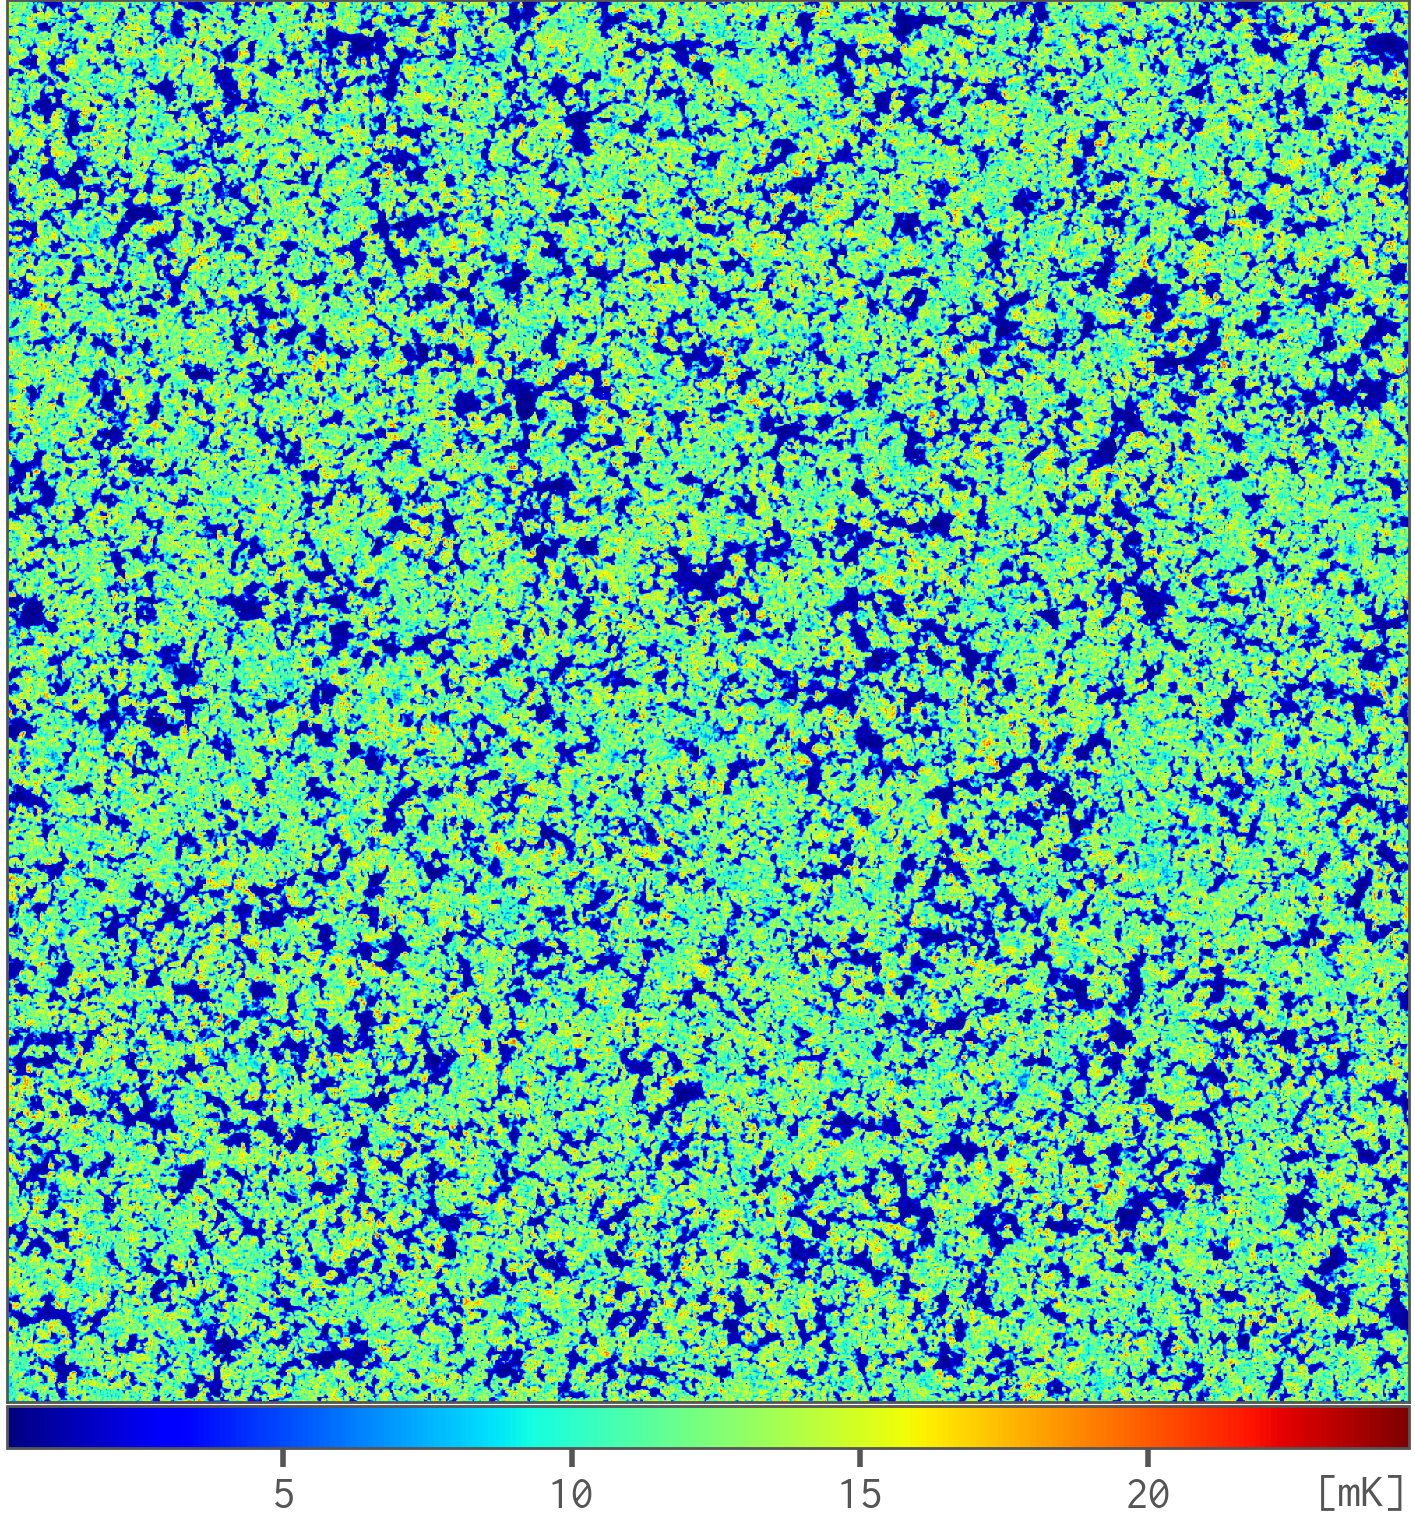
\includegraphics[width=0.7\textwidth]{skymap-eor-f158}
  \bicaption[EoR 信号在 \SI{158}{\MHz} 的天图]{%
    TODO...
  }{%
    The sky map of the EoR signal at \SI{158}{\MHz}.
    The sky region size is \SI{10 x 10}{\degree}
    and the color bar is in units of \si{\mK}.
  }
  \label{fig:eor-skymap}
\end{figure}


%=====================================================================
\section{干涉阵列的模拟观测}
\label{sec:obs-simu}

In order to properly evaluate the contamination of radio halos
on the EoR observations, it is essential to take account of the
practical instrumental effects of radio interferometers.

%---------------------------------------------------------------------
\subsection{SKA1-Low~阵列布局}

TODO: layout configuration, design goals, descriptions, figures...

Therefore, we employ the latest SKA1-Low layout configuration%
\footnote{\raggedright%
  SKA1-Low Configuration Coordinates:
  \url{https://astronomers.skatelescope.org/wp-content/uploads/2016/09/SKA-TEL-SKO-0000422_02_SKA1_LowConfigurationCoordinates-1.pdf}
  (released on 2016 May 21)
}
to simulate the SKA observations of the above simulated sky maps.
According to this layout configuration,
the SKA1-Low interferometer consists of 512 stations, with 224 of them
randomly distributed within the \enquote{core} of \SI{1000}{\meter} in
diameter, while the remaining stations are grouped into \enquote{clusters}
and placed on 3 spiral arms extending up to a radius of
\SI{\sim 35}{\kilo\meter}.
Each station has 256 antennas randomly distributed with a minimum separation
of $d_{\R{min}} = \SI{1.5}{\meter}$ inside a circular region of
\SI{35}{\meter} in diameter \cite{mort2017}.

%---------------------------------------------------------------------
\subsection{模拟观测和成像}

The \SI{8}{\MHz} bandwidth of each frequency band is divided into 51
channels for a frequency resolution of \SI{160}{\kilo\hertz}.
For each component, we simulate the input sky maps at every frequency
channel, and then use the
\href{https://github.com/OxfordSKA/OSKAR}{\texttt{OSKAR}}\footnote{%
  OSKAR: \url{https://github.com/OxfordSKA/OSKAR} (version 2.7.0)}
simulator \cite{mort2010} to perform observations for \SI{6}{\hour}.
The input sky maps are centered at sky position of
(R.A., Dec.\@) = (\SI{0}{\degree}, \SI{-27}{\degree}),
which passes through the zenith of the SKA1-Low telescope and
is an ideal choice for the simulation of SKA observations.
The simulated visibility data are imaged through the
\href{https://sourceforge.net/p/wsclean}{\texttt{WSClean}}\footnote{%
  WSClean: \url{https://sourceforge.net/p/wsclean} (version 2.6)}
imager \cite{offringa2014} using Briggs' weighting with a
robustness of zero \cite{briggs1995},
and the created images are cropped to keep only the central regions
because the marginal regions suffer from the problem of insufficient
CLEAN.
As the telescope's field of view (FoV) is inversely proportional to
the observing frequency, we choose to keep the central
\SI{6 x 6}{\degree}, \SI{5 x 5}{\degree}, and \SI{4 x 4}{\degree}
regions in the \numrange{120}{128}, \numrange{154}{162}, and
\numrange{192}{200} \si{\MHz} frequency bands, respectively.

The Galactic synchrotron and free-free emissions are combined for the
simulated observations because they have similar diffuse features.
Similar to the real-time peeling of the brightest point sources in
practical data analysis pipelines
\cite{mitchell2008,intema2009,mort2017},
we assume that extragalactic point sources with a \SI{158}{\MHz} flux
density $S_{158} > \SI{50}{\mJy}$ are removed
\cite{liu2009ps,pindor2011}.
Thus, the root-mean-square brightness temperatures of point sources
are significantly reduced to be about
\num{22.5e4}, \num{9.81e4}, and \num{4.75e4} \si{\mK}
at 124, 158, and 196 \si{\MHz}, respectively.
In addition, we create the foreground image cubes in each frequency band
using the CLEAN algorithm with joined-channel deconvolution in order
to ensure the spectral smoothness \cite{offringa2017}, which is crucial
to extract the faint EoR signal in the presence of overwhelming
foreground contamination.
For the EoR signal, we directly use the dirty images because the CLEAN
algorithm is not well applicable to such faint and diffuse emissions.
Hence we obtain the SKA \enquote{observed} image cubes of the EoR signal,
radio halos, the Galactic diffuse emission (with synchrotron and
free-free emissions combined), and the extragalactic point sources
(with the brightest ones removed) in the \numrange{120}{128},
\numrange{154}{162}, and \numrange{192}{200} \si{\MHz} frequency bands.


%=====================================================================
\section{小结}

TODO


%% EOF

%%
%% Copyright (c) 2018-2019 Weitian LI <liweitianux@sjtu.edu.cn>
%% Creative Commons BY 4.0
%%

\chapter{射电晕对宇宙再电离探测的影响}
\label{chap:halo}

%=====================================================================
\section{评估方法}

利用\autoref{chap:simulation}模拟得到的射电晕、EoR 信号以及其他前景成分的
SKA1-Low 观测图像,我们可以定量地评估射电晕将对 EoR 探测产生的影响.
我们将分别针对\ac{fgrm}和\ac{fgavd}两类前景处理方法 (\autoref{sec:fg-methods})
进行评估.
首先,我们计算一维\ac{ps}来对比射电晕和 EoR 信号在各个尺度 $k$ 的总体功率,
说明使用\ac{fgrm}方法时将面临的射电晕的污染强度.
其次,我们计算二维\ac{ps},然后在 EoR 窗口 (\autoref{sec:eor-window})
内比较射电晕和 EoR 信号的功率,
据此评估射电晕的污染将会对使用\ac{fgavd}方法产生多大程度的影响.

\begin{figure}[htp]
  \centering
  \includegraphics[width=\textwidth]{ft-sidelobes}
  \bicaption[加窗前后的 Fourier 变换结果对比]{%
    直接进行 Fourier 变换(红色实线)与
    使用 Blackman--Nuttall \acs*{winfunc}之后再 Fourier 变换(蓝色虚线)
    的结果对比.
    左栏显示了加窗前后的输入信号 $y = (x/158)^{-2}$,
    右栏显示了相应的 Fourier 变换结果.
  }{%
    A comparison of the Fourier transform results with and without
    applying the Blackman--Nuttall window function.
    The left panel shows the original input signal $y = (x/158)^{-2}$
    (solid red line) and the windowed signal (dashed blue line);
    the right panel shows the corresponding Fourier transform results.
  }
  \label{fig:ft-sidelobes}
\end{figure}

考虑一个有限宽的频带,信号(如前景辐射)将在频带的两端出现跃变,
这种边界效应会导致 Fourier 变换的结果具有显著的\ac{sidelobe}.
即使输入信号非常平滑,Fourier 变换后也会出现一系列幅度较大的高频 Fourier 成分,
如\autoref{fig:ft-sidelobes} 所示.
为了抑制边界效应所产生的\ac{sidelobe},可以先对信号加窗,然后再进行 Fourier 变换.
一个常用的选择是 Blackman--Nuttall \ac{winfunc},
该\ac{winfunc}具有良好的\ac{sidelobe}性质 \cite{nuttall1981}:
\begin{equation}
  w[n] = a_0 - a_1 \cos\left(\frac{2\Cpi n}{N}\right)
    + a_2 \cos\left(\frac{4\Cpi n}{N}\right)
    - a_3 \cos\left(\frac{6\Cpi n}{N}\right) ,
\end{equation}
其中
$N$ 为采样点的数目(即窗的宽度),
其他系数分别为:
$a_0 = \num{0.3635819}$,
$a_1 = \num{0.4891775}$,
$a_2 = \num{0.1365995}$,
$a_3 = \num{0.0106411}$.
\autoref{fig:ft-sidelobes} 显示了使用 Blackman--Nuttall \ac{winfunc}
之后得到的 Fourier 变换结果,可见高频 Fourier 成分的幅度被有效地抑制了.
因此,我们对\autoref{chap:simulation}模拟得到的\ac{imgcube}沿频率方向施加
Blackman--Nuttall \ac{winfunc}然后再计算\ac{ps}
\cite{trott2015,chapman2016}.


%=====================================================================
\section{一维功率谱}
\label{sec:ps1d}

\begin{figure}[htp]
  \centering
  \includegraphics[width=\textwidth]{ps1d-3bands}
  \bicaption[各成分在三个频带内的一维功率谱 $\ac{psD}(k)$ 对比]{%
    EoR 信号(绿色实线)、射电晕(红色实线)、银河系弥散辐射(灰色虚线)以及
    河外点源(灰色点虚线)之间的一维功率谱 $\ac{psD}(k)$ 的对比.
    左栏、中栏、右栏分别表示 \numrange{120}{128}、\numrange{154}{162}
    和 \numrange{192}{200} \si{\MHz} 三个频带的结果.
    对于射电晕,红色实线及其阴影区域分别表示从 100 次模拟结果中得到的
    中位数和 68\% 的误差范围.
  }{%
    Comparisons of the 1D dimensionless power spectra $\ac{psD}(k)$
    among the EoR signal (solid green line), radio halos (solid red line),
    Galactic diffuse emission (dashed gray line), and extragalactic point
    sources (dash-dotted gray line) in the
    \textbf{(a)} \SIrange{120}{128}{\MHz},
    \textbf{(b)} \SIrange{154}{162}{\MHz}, and
    \textbf{(c)} \SIrange{192}{200}{\MHz} frequency bands.
    The solid red lines and shaded regions represent the median values
    and the corresponding 68\% uncertainties of the power
    spectra for radio halos estimated from the 100 simulation runs.
  }
  \label{fig:ps1d-3bands}
\end{figure}

我们对上一章模拟得到的每一个成分在每一个频带里的\ac{imgcube}分别计算了
一维\ac{ps} $\ac{psD}(k)$.
对于射电晕,我们使用了全部 100 次模拟 (\autoref{sec:halo-maps}) 的结果
来估算其一维功率谱的中位数和 68\% 的误差范围.
具体而言,在一个频带里,射电晕的 100 次模拟会生成 100 个\ac{imgcube},
分别计算这 100 个\ac{imgcube}的一维功率谱,
然后从所得的 100 个一维功率谱计算每个尺度 $k$ 处的中位数和相应的 68\% 误差范围.
\autoref{fig:ps1d-3bands} 显示了各成分在三个频带内的
一维功率谱 $\ac{psD}(k)$ 的对比.
可见,在 $\SI{0.1}{\per\Mpc} < k < \SI{2}{\per\Mpc}$ 尺度上,
射电晕的典型功率(红色实线)在 \numrange{120}{128}、\numrange{154}{162} 和
\numrange{192}{200} \si{\MHz} 频带内分别是 EoR 信号的功率的
\num{e4}、\num{e3} 和 \num{e2.5} 倍.
考虑到不同天区内射电晕的亮度和数目的显著涨落,
在 68\% 的误差范围内(红色阴影区域),
射电晕的功率能够变化约 \numrange{10}{100} 倍.

对于另外两个前景成分,银河系前景在最大尺度 ($k \lesssim \SI{0.1}{\per\Mpc}$)
上是最强的污染源,但随着尺度 $k$ 的减小,其功率也迅速减小.
在 $\SI{0.5}{\per\Mpc} \lesssim k \lesssim \SI{1}{\per\Mpc}$
的中小尺度范围,
射电晕的典型功率将是银河系前景的功率的约 \numrange{10}{100} 倍.
河外点源除了在最大尺度上弱于银河系前景,在其他尺度上均是最强的污染源.

以上这些结果清楚地说明射电晕是严重的 EoR 前景污染源,需要在前景扣除中被仔细处理.
此外,射电晕还具有一定的形态结构,显著增加了对其准确建模和扣除的难度.


%=====================================================================
\section{二维功率谱}
\label{sec:ps2d}

\begin{figure}[htp]
  \centering
  \includegraphics[width=\textwidth]{ps2d-band158}
  \bicaption[%
    各成分在 \SIrange{154}{162}{\MHz} 频段的二维功率谱
    $\ac{psD}(\kperp, \klos)$%
  ]{%
    各成分在 \SIrange{154}{162}{\MHz} 频段的二维功率谱
    $\ac{psD}(\kperp, \klos)$,
    从左上至右下分别为:
    \textbf{(a)} EoR 信号;
    \textbf{(b)} 射电晕(100 次模拟的中位数);
    \textbf{(c)} 银河系弥散辐射;
    \textbf{(d)} 河外点源.
    所有子图共用了以 [\si{\mK\squared\Mpc\cubed}] 为单位的对数\ac{colorbar}.
    图中的白色虚线显示了 EoR 窗口的边界.
  }{%
    The \SIrange{154}{162}{\MHz} 2D power spectra
    $\ac{psD}(\kperp, \klos)$ of
    \textbf{(a)} the EoR signal,
    \textbf{(b)} radio halos (median of the 100 simulation runs),
    \textbf{(c)} Galactic diffuse emission,
    and
    \textbf{(d)} extragalactic point sources.
    All panels share the same logarithmic scale in units of
    [\si{\mK\squared\Mpc\cubed}].
    The dashed white lines mark the boundary between the EoR window
    (at the top left) and the contaminating wedge (at the bottom right).
  }
  \label{fig:ps2d}
\end{figure}

以 \SIrange{154}{162}{\MHz} 频带为例,
\autoref{fig:ps2d} 显示了 EoR 信号、射电晕、银河系弥散辐射以及河外点源的
二维功率谱 $\ac{psD}(\kperp, \klos)$,
其中射电晕的二维功率谱对应于 100 次模拟结果的中位数.
从图中容易看出,EoR 信号的功率分散在大范围的 \klos{} 模式上,
反映了 EoR 信号沿频率维度快速变化的特点;
频谱光滑的前景成分则集中在 \klos{} 较小的区域
($\klos{} \lesssim \SI{0.2}{\per\Mpc}$).
在空间维度 \kperp{},射电晕的功率主要出现在
$\kperp \lesssim \SI{1}{\per\Mpc}$ 的范围,
并且倾向于集中在 $\kperp \sim \SI{0.5}{\per\Mpc}$ 的中等尺度上.
同时,银河系弥散辐射的功率主导了 $\kperp \lesssim \SI{0.1}{\per\Mpc}$
的大尺度区域,而河外点源的功率则占据了 $\kperp \gtrsim \SI{0.1}{\per\Mpc}$
的中小尺度范围.
这些结果与 \autoref{fig:ps1d-3bands}(b) 所展示的结果是相符的,
还与诸多文献中的结果是一致的 \cite{datta2010,trott2015,barry2016,chapman2016}.

\begin{figure}[htp]
  \centering
  \includegraphics[width=\textwidth]{ps2d-ratio-3bands}
  \bicaption[射电晕和 EoR 信号的二维功率比 $R(\kperp, \klos)$]{%
    射电晕和 EoR 信号在
    \textbf{(a)} \SIrange{120}{128}{\MHz}、
    \textbf{(b)} \SIrange{154}{162}{\MHz} 和
    \textbf{(c)} \SIrange{192}{200}{\MHz}
    三个频带内的二维功率比 $R(\kperp, \klos)$.
    这里使用的射电晕二维功率谱对应于 100 次模拟结果的中位数.
    所有子图共用了对数\ac{colorbar}.
    图中的白色虚线显示了 EoR 窗口的边界.
  }{%
    The 2D power spectrum ratios $R(\kperp, \klos)$ of radio halos to the
    EoR signal in the
    \textbf{(a)} \SIrange{120}{128}{\MHz},
    \textbf{(b)} \SIrange{154}{162}{\MHz}, and
    \textbf{(c)} \SIrange{192}{200}{\MHz} frequency bands.
    The median 2D power spectrum of 100 simulation runs for radio halos
    is used.
    All panels use the same color bar in logarithmic scale.
    The dashed white lines mark the EoR window boundaries.
  }
  \label{fig:ps2d-ratio}
\end{figure}

为了更具体地显示射电晕对 EoR 信号的污染情况,
我们将射电晕的二维功率谱除以 EoR 信号的二维功率谱,
得到两者的二维功率比 $R(\kperp, \klos)$,如\autoref{fig:ps2d-ratio} 所示,
可见射电晕的污染区域形成一个明显的楔形 (\autoref{sec:eor-window}).
我们发现,在 \SIrange{120}{128}{\MHz} 频带内,
射电晕在 $\kperp \gtrsim \SI{0.1}{\per\Mpc}$ 的尺度范围内
对 EoR 信号产生了严重污染(两者功率比值 $R \gtrsim 1$).
在 \numrange{154}{162} 和 \numrange{192}{200} \si{\MHz} 两个频带里,
射电晕的主要污染范围分别为 $\kperp \gtrsim \SI{0.3}{\per\Mpc}$
和 $\kperp \gtrsim \SI{0.5}{\per\Mpc}$.
同时容易看出,射电晕在较低频率处 (\SI{\sim 120}{\MHz})
对 EoR 测量的污染程度明显比在较高频率处 (\SI{\sim 200}{\MHz})
的污染程度要强.
\autoref{fig:ps1d-3bands} 也显示了与此一致的结果.

\begin{figure}[htp]
  \centering
  \includegraphics[width=0.8\textwidth]{ps1d-ratio-3bands}
  \bicaption[射电晕和 EoR 信号在 EoR 窗口内的一维功率比 $R_{\R{eorw}}(k)$]{%
    射电晕和 EoR 信号在 EoR 窗口内的一维功率比 $R_{\R{eorw}}(k)$.
    实线和阴影区域分别对应于射电晕 100 次模拟结果的中位数和 68\% 误差范围.
  }{%
    The 1D power ratios $R_{\R{eorw}}(k)$ inside the EoR window of
    radio halos to the EoR signal.
    The solid lines and shaded regions show the median values and
    corresponding 68\% uncertainties, respectively.
  }
  \label{fig:ps1d-ratio}
\end{figure}

考虑到射电晕的污染主要集中在二维功率谱右下方的楔形区域内
(如\autoref{fig:ps2d-ratio} 所示),
因此可以选定一个合适的边界将其排除,
于是便可以在左上方的 EoR 窗口内提取 EoR 信号,
有效地避开了强烈的前景污染,这就是\ac{fgavd}方法的基本思路.
利用\autoref{eq:eor-window} 定义的 EoR 窗口边界的表达式,
我们测试了多种不同的 ($w$, $\Phi$) 参数组合,
最终选择了 $w = 3$ 以及 $\Phi = 1.5\,\ac{Fov}$,
即 $\Phi$ 在 \numrange{120}{128}、\numrange{154}{162}
和 \numrange{192}{200} \si{\MHz} 三个频带的值分别为
$\Phi_{124} = \SI{7.5}{\degree}$、
$\Phi_{158} = \SI{6.0}{\degree}$ 和
$\Phi_{196} = \SI{4.8}{\degree}$.
\autoref{fig:ps2d} 和\autoref{fig:ps2d-ratio} 显示了如此定义的 EoR 窗口边界,
可见能够很好地避开\ac{fg-wedge}的污染.
但是,在 \numrange{120}{128}、\numrange{154}{162}
和 \numrange{192}{200} \si{\MHz} 三个频带内,
EoR 信号分别有约 55\%、54\% 和 40\% 的功率损失在避开的\ac{fg-wedge}之中.

在以上定义的 EoR 窗口内,对射电晕和 EoR 信号的二维功率比 $R(\kperp, \klos)$ 平均,
得到一维功率比 $R_{\R{eorw}}(k)$,如\autoref{fig:ps1d-ratio} 所示.
相比\autoref{fig:ps1d-3bands} 所示的未受 EoR 窗口约束的一维功率谱 $\ac{psD}(k)$,
射电晕的污染在 EoR 窗口内被抑制了约 4 个数量级.
比如,在 $k \sim \SI{1}{\per\Mpc}$ 尺度上,
EoR 窗口内的一维功率比 $R_{\R{eorw}}(k)$ 在 \numrange{120}{128}、
\numrange{154}{162} 和 \numrange{192}{200} \si{\MHz}
三个频带的典型值(图中的实线)分别约为 45\%、6\% 和 2\%.
这充分展示了 EoR 窗口和\ac{fgavd}法是探测 EoR 信号的有力工具.
尽管如此,由于射电晕的亮度和数目在不同天区里具有显著的涨落,
在 68\% 的误差范围(图中的阴影区域)以及
$\SI{0.5}{\per\Mpc} \lesssim k \lesssim \SI{1}{\per\Mpc}$ 尺度范围内,
EoR 窗口内的一维功率比 $R_{\R{eorw}}(k)$ 在三个频带内的值能够分别达到约
\numrange{230}{800}\%、\numrange{18}{95}\% 和 \numrange{7}{40}\%,
说明射电晕泄漏到 EoR 窗口内的功率仍然可能是显著的,
尤其是在较低频率 (\SI{\sim 120}{\MHz}).

基于本节和上一节 (\autoref{sec:ps1d}) 的结果,
我们认为射电晕是 EoR 信号探测的一个重要前景干扰成分.
即使在一个已避开严重污染的 EoR 窗口内,射电晕所产生的污染仍然能够
对 EoR 信号的准确测量产生不可忽略的干扰,尤其是在 \SI{\sim 120}{\MHz} 的较低频率.
为了获得一个尽可能干净、同时也尽可能大的 EoR 窗口,
深入理解、建模并扣除射电晕以及其他前景干扰成分是非常必要的,
还需要联合使用\ac{fgrm}和\ac{fgavd}两类方法,改进 EoR 信号探测手段.


%=====================================================================
\section{伪频谱结构的影响}
\label{sec:freq-artifacts}

In practical observations with low-frequency radio interferometers, the
situations are much more complicated than our simulations.
For example, calibration uncertainties (e.g., insufficient sky modeling)
as well as other complicated instrumental and observational effects
(e.g., cable signal reflections, ionospheric distortions) can cause
frequency artifacts in the derived image cubes.

The smoothness along the frequency dimension is the most crucial feature
of various foreground components and is the key to extract the faint EoR
signal.
However, frequency artifacts may present in the obtained image cubes due
to calibration uncertainties and various instrumental and observational
effects, which break the spectral smoothness of the foreground emission
and hence damage the EoR measurements.

To evaluate the influence of the frequency artifacts on the power
spectra, we multiply each slice of the image cube by a random number
drawn from a Gaussian distribution with unity mean and then compare
the resulting power spectra \cite{chapman2016}.
Some simulation and observation studies have suggested that the residual
calibration errors in frequency channels may be about \numrange{0.1}{1}\%
\cite{barry2016,beardsley2016,ewallWice2017}.
We thus investigate two extreme cases here:
a frequency artifact of amplitude $A_{\R{arti}} = 0.1\%$ by
using $\sigma = 0.001$ for the Gaussian distribution,
and a frequency artifact of $A_{\R{arti}} = 1\%$ with $\sigma = 0.01$.

\begin{figure}[htp]
  \centering
  \includegraphics[width=0.75\textwidth]{ps2d-ratio-crp-3bands}
  \bicaption[有无频谱伪结构时射电晕的二维功率比 $R_{\R{arti}}(\kperp, \klos)$]{%
    有无频谱伪结构时射电晕的二维功率比 $R_{\R{arti}}(\kperp, \klos)$.
    上、中、下三行分别对应 \numrange{120}{128}、\numrange{154}{162} 和
    \numrange{192}{200} \si{\MHz} 三个频带;
    左、右两列分别显示了频谱伪结构幅度为 $A_{\R{arti}} = 0.1\%$
    和 $A_{\R{arti}} = 1\%$ 的情况;
    白色虚线标识了 EoR 窗口的边界.
    所有子图共用了对数\ac{colorbar}.
  }{%
    The 2D power spectrum ratios $R_{\R{arti}}(\kperp, \klos)$
    of radio halos with and without frequency artifacts.
    The upper, middle, and lower rows show the power spectrum ratios
    in the \numrange{120}{128}, \numrange{154}{162}, and
    \numrange{192}{200} \si{\MHz} bands, respectively;
    the left and right columns show the cases of frequency artifacts
    being $A_{\R{arti}} = 0.1\%$ and $A_{\R{arti}} = 1\%$, respectively.
    The dashed white lines mark the EoR window boundaries.
    All panels share the same color bar in logarithmic scale.
  }
  \label{fig:ps2d-ratio-crp}
\end{figure}

For each of the 100 simulation runs for radio halos, we calculate the
2D power spectrum ratios $R_{\R{arti}}(\kperp, \klos)$ of the modified
image cube with the frequency artifact to the original one
(\autoref{sec:obs-simu}),
and present the median 2D power spectrum ratios obtained in the
\numrange{120}{128}, \numrange{154}{162}, and \numrange{192}{200}
\si{\MHz} bands with either $A_{\R{arti}} = 0.1\%$ or 1\% in
\autoref{fig:ps2d-ratio-crp}.
We find that, when the frequency artifact is added, the resulting 2D
power spectra are seriously damaged in all three frequency bands.
On scales of $\kperp \lesssim \SI{0.2}{\per\Mpc}$ and
$\klos \gtrsim \SI{0.3}{\per\Mpc}$,
adding frequency artifact of $A_{\R{arti}} = 0.1\%$
causes the power of radio halos to be about 17, 15, and 13 times
stronger in the \numrange{120}{128},
\numrange{154}{162}, and \numrange{192}{200} \si{\MHz} bands,
respectively, and the corresponding power increases are about
1700, 1500, and 1300 times
for frequency artifact of $A_{\R{arti}} = 1\%$.
As a comparison, we add the same frequency artifacts
($A_{\R{arti}} = 0.1\%$ and 1\%) to the image
cubes of the EoR signal, but find that the changes in the calculated
2D power spectra are negligible.
This is because the EoR signal already fluctuates remarkably along
the frequency dimension.
Consequently, even very minor (\num{\sim 0.1}\%) instrumental or
calibration errors can make the contamination of radio halos
become much stronger, particularly inside the critical EoR window.
These results further support our conclusion made in \autoref{sec:ps2d}
that radio halos are important foreground sources and must be carefully
dealt with in EoR experiments.


%=====================================================================
\section{远旁瓣的影响}
\label{sec:fscn}

Phased arrays, which are widely used in low-frequency radio
interferometers (e.g., LOFAR, MWA, SKA1-Low), usually have complicated
beam profiles.
Sources far from the main lobe of the station beam can introduce
noise-like corruptions, known as the far side-lobe confusion noise
(FSCN; \citeay{smirnov2012}), to images through the multitude of
side-lobes.
FSCN will not decrease once the $uv$ coverage of the observation no
longer improves, and can be the limiting factor in the noise
performance of interferometers \cite{mort2017}.

To investigate the impacts of FSCN contributed by the radio halos
located in the far side-lobes of the station beam, we have generated
the corresponding sky model for the \texttt{OSKAR} simulator,
which evaluates the radio interferometer measurement equation
\cite{smirnov2011} and is able to perform full-sky simulations with
realistic beam profiles.
More details about the beam shapes and side-lobe properties of the
SKA1-Low can be found in \citeay{mort2017}.
As an example, we simulate the radio halos in the \SIrange{154}{162}{\MHz}
band that cover the sky from the edge of the second side-lobe
($\phi \sim \SI{10}{\degree}$ from the field center) to the horizon
($\phi = \SI{90}{\degree}$).
This emulates an ideal CLEAN procedure in practical data analysis that
removes all the radio halos in both the main lobe and the first side-lobe
but leaves the ones in the far side-lobes.
Using the \texttt{OSKAR} simulator and the \texttt{WSClean} imager as
described in \autoref{sec:obs-simu}, we obtain the dirty images of the
central \SI{5 x 5}{\degree} region and then
calculate the 2D power spectrum.

\begin{figure}[htp]
  \centering
  \includegraphics[width=\textwidth]{ps2d-fscn}
  \bicaption[射电晕 FSCN 的二维功率谱及其与 EoR 信号的功率谱对比]{%
    \emph{(a)} 射电晕 FSCN 的二维功率谱 $\Delta^2_{\R{fscn}}(\kperp, \klos)$;
    \emph{(b)} 射电晕 FSCN 与 EoR 信号的二维功率比 $R_{\R{fscn}}(\kperp, \klos)$.
    白色虚线和实线分别标识了 $\Phi = \SI{6}{\degree}$ 和 \SI{90}{\degree}
    所对应的 EoR 窗口边界.
  }{%
    \emph{(a)} The 2D power spectrum of the FSCN caused by radio halos
    in the far side-lobes of the station beam.
    \emph{(b)} The 2D power spectrum ratio of the FSCN to the EoR signal.
    The results are derived in the \SIrange{154}{162}{\MHz} band.
    The dashed and solid white lines mark the EoR window boundaries
    defined with $\Phi = \SI{6}{\degree}$ and \SI{90}{\degree},
    respectively.
  }
  \label{fig:ps2d-fscn}
\end{figure}

In \autoref{fig:ps2d-fscn}, we present the 2D power spectrum of the FSCN
contributed by radio halos and the corresponding 2D power spectrum ratio
of the FSCN to the EoR signal.
We find that the FSCN contamination is very strong as its power can be
about 20 times the power of the EoR signal on scales of
$\kperp \sim \SI{0.3}{\per\Mpc}$ and $\klos \sim \SI{1.0}{\per\Mpc}$.
The wedge-shaped contamination region moves toward the top left in
the $(\kperp, \klos)$ plane and greatly reduces the EoR window.
In order to effectively avoid the FSCN contamination, we are forced to
employ a much more conservative EoR window boundary, such as the one
defined with $\Theta = \SI{90}{\degree}$ as marked in
\autoref{fig:ps2d-fscn} with solid white line, at the cost of losing
a remarkably larger portion of the EoR signal.
In consequence,
the serious FSCN contamination makes the selection of EoR sky region
a more challenging task, since in principle neither bright radio halos
nor other strong sources are allowed in both the main and side lobes.
A highly accurate foreground model is hence crucial to mitigate the
impacts of FSCN.


%=====================================================================
\section{小结}

Based on the Press--Schechter formalism and merger-induced turbulent
re-acceleration model, we have simulated the emission maps of radio halos,
for which we have incorporated the SKA1-Low's instrumental effects by
utilizing its latest layout configuration.
By carrying out detailed comparisons of power spectra between radio halos
and the EoR signal as well as the Galactic diffuse emission and
extragalactic point sources in the \numrange{120}{128},
\numrange{154}{162}, and \numrange{192}{200} \si{\MHz} bands,
we have shown that radio halos are severe contaminating sources,
especially toward lower frequencies (\SI{\sim 120}{\MHz}).
Even if inside the properly defined EoR windows, radio halos can still
be non-negligible contaminating sources to EoR observations.
Moreover, we have investigated the contamination resulted from
frequency artifacts and radio halos located inside the far side-lobes,
both of which support our conclusion that radio halos are severe
foreground contaminating sources and need careful treatments in the
forthcoming deep EoR observations.

此工作已发表于 \apj{} (ApJ)\reviewornot{}{\cite{li.halo}}.


%% EOF

%%
%% Copyright (c) 2018-2019 Weitian LI <liweitianux@sjtu.edu.cn>
%% Creative Commons BY 4.0
%%

\chapter{基于深度学习的再电离信号分离新算法}
\label{chap:cdae}

为了能够从强烈的前景干扰中分离出微弱的 EoR 信号,
传统的\ac{fgrm}方法都依赖于一个关键的前提:
前景干扰具有非常光滑的频谱,而 EoR 信号沿频率维度发生剧烈变化,
两者具有显著不同的频谱结构,从而能够被有效地分离开 \cite{morales2010,chapman2016}.
然而,在实际情况中,未分辨的或者未完全扣除的干扰源在干涉阵列的波束效应的影响下,
会在频率维度产生震荡形式的辐射,破坏前景频谱的光滑性 \cite{liu2009ps}.
这会显著削弱前景干扰与 EoR 信号的可分性,
导致传统\ac{fgrm}方法的效果大打折扣甚至失效,
因此需要研发能够克服波束效应的 EoR 信号分离新算法.


%=====================================================================
\section{波束的频率依赖效应}
\label{sec:beam-effect}

\begin{figure}[htp]
  \centering
  \includegraphics[width=\textwidth]{SKA1-low-psf}
  \bicaption[模拟的 SKA1-Low 综合波束]{%
    在 154、158 和 162 MHz 处模拟的 SKA1-Low \acs*{beam-synthesized}.
    积分时间为 \SI{6}{\hour}.
  }{%
    The simulated synthesized beams of SKA1-Low at 154, 158, and 162 MHz.
    The integration time is \SI{6}{\hour}.
  }
  \label{fig:ska-psf}
\end{figure}

一个干涉阵列拥有的\ac{baseline}的数目和长度均是有限的,
在观测中能实现的 $uv$ 覆盖也是有限而且不完备的 (\autoref{sec:uv-coverage}),
因此,干涉阵列的\ac{beam-synthesized}的形状非常复杂.
如\autoref{fig:ska-psf} 所示,
除了中间一个很窄的\ac{mainlobe},\ac{beam-synthesized}还包含一系列\ac{sidelobe}.
这些\ac{sidelobe}的数量非常多,相对幅度约为 \numrange{0.01}{0.1}\%,
一直延伸到远超出视场的位置.
另见 \citeay{liu2009ps} 的图 1 和图 3.

另一方面,\ac{beam-synthesized}的形状还依赖于观测频率.
\ac{sidelobe}的位置 $\theta$ 会随着频率 $\nu$ 的增大而向中间移动,
即 $\theta \propto \nu^{-1}$.
因此,一个干扰源在视场中所产生的辐射的位置也随频率而变化.
由于仪器的热噪声水平、成像的天区大小、CLEAN 的深度等因素的限制,
视场中总是存在一批未分辨的以及未完全扣除而残留的干扰源.
由这些干扰源的辐射综合而成的前景干扰,
在频率维度将出现类似\ac{beam-synthesized}的\ac{sidelobe}形状的起伏.
这将破坏前景辐射的频谱光滑性,使得前景干扰具有类似 EoR 信号的小尺度频谱结构,
导致传统\ac{fgrm}方法无法有效地将两者区分开.
另见 \citeay{liu2009ps} \S\,1.


%=====================================================================
\section{基于深度学习的新算法}

传统方法的严重不足,
机器学习/深度学习方法的必要性,
从数据中学习, 灵活性/自适应/泛化/可扩展

Given the complicated profiles and frequency-dependent variations of
the PSF, it would be very difficult to craft a practicable model for most,
if not all, existing foreground removal methods to overcome the beam
effects, even at the cost of extensive computation burden
\cite{lochner2015}.
Therefore, deep-learning-based methods, which can distil knowledge from
the data to automatically refine the model, seem more feasible
and appealing \cite{herbel2018,vafaeiSadr2019}.
In recent years, deep learning algorithms have seen prosperous
developments and have brought breakthroughs into many fields
(see \citeay{lecun2015} for a recent review).
Among various deep learning algorithms, the autoencoder is a common type of
neural networks that aims at learning useful features from the input data
in an unsupervised manner, and it is usually used for dimensionality
reduction \cite{hinton2006,wang2014} and data denoising
\cite{xie2012,lu2013,bengio2013}.
In particular,
the convolutional denoising autoencoder (CDAE) is very flexible and
powerful in capturing subtle and complicated features in the data and have
been successfully applied to weak gravitational wave signal denoising
\cite{shen2017}, monaural audio source separation
\cite{grais2017}, and so on.
These applications have demonstrated the outstanding abilities of the
CDAE in extracting weak signals from highly temporal-variable data.
Thus it is worth trying to apply the CDAE to separate the EoR signal.
Although the signal-to-noise ratio in the EoR separation task is much lower
than in existing applications, the EoR signal and foreground emission as
well as the beam effects are stationary or semi-stationary.

%---------------------------------------------------------------------
\subsection{深度学习简介}

TODO...

%---------------------------------------------------------------------
\subsection{卷积去噪自编码器}
\label{sec:cdae}

An autoencoder is composed of an encoder and a decoder, which can be
characterised by the functions $f(\cdot)$ and $g(\cdot)$, respectively.
The encoder maps the input $\B{x}$ to an internal code $\B{h}$, i.e.,
$\B{h} = f(\B{x})$, and the decoder tries to reconstruct the desired
signal from the code $\B{h}$, i.e., $\B{r} = g(\B{h})$, where $\B{x}$,
$\B{h}$, and $\B{r}$ are all vectors in this work.
By placing constraints (e.g., dimensionality, sparsity) on the
code $\B{h}$ and training the autoencoder to minimize the
loss $L(\B{r}, \,\B{x})$, which quantifies the difference between the
reconstruction $\B{r}$ and the input $\B{x}$, the autoencoder is expected
to learn the codes that effectively represent the input
(详见 \citeay{goodfellow2016},第 14 章).

In order to make the autoencoder learn a better representation of the input
to achieve better performance, \citet{vincent2008} and \citet{vincent2010} proposed a
novel training strategy based on the denoising criterion:
artificially corrupt the original input $\B{x}$ (e.g., by adding noise),
feed the corrupted input $\B{x}'$ into the autoencoder, and then train it
to reconstruct the original input $\B{x}$ by minimizing the loss
$L(\B{r}, \,\B{x})$.
During this denoising process, the autoencoder is
forced to capture robust features that are critical to accurately
reconstruct the original input.
An autoencoder trained with such a strategy
is called a `denoising autoencoder.'

Classic autoencoders are built with fully connected layers, each neuron of
which is connected with every neuron in the previous layer.
This makes the total number of parameters increase exponentially with the
number of layers.
Meanwhile, the extracted features are forced to be global, which
is suboptimal to represent the input \cite{masci2011}.
On the other hand, convolutional layers, as used in convolutional neural
networks (CNNs),
make use of a set of small filters and share their weights among
all locations in the data \cite{lecun1998}, which allows to
better capture the local features in the data.
Therefore, CNNs generally have two or more orders of magnitude less
parameters than the analogous fully connected neural networks
\cite{grais2017}
and require much less training resources such as memory and time.
Furthermore, multiple convolutional layers can be easily stacked to extract
sophisticated higher-level features by composing the lower-level ones
obtained in previous layers.
This technique guarantees highly expressive CNNs that achieve
outstanding performance in image classification and relevant fields
\cite{krizhevsky2012,simonyan2014,szegedy2015,ma2019}.
By utilising multiple convolutional layers instead of fully connected
layers in a denoising autoencoder, the obtained CDAE gains the powerful
feature extraction capability of CNNs, which helps improve its denoising
performance, and can reconstruct even seriously corrupted signals
\cite{du2017}.
In consequence, the CDAE may be well suited to exploit the complicated
differences between the EoR signal and the foreground emission
for the purpose of separating them accurately.

%---------------------------------------------------------------------
\subsection{网络架构}
\label{sec:architecture}

Both the encoder and decoder parts of the proposed CDAE consist of multiple
convolutional layers.
We do not set a strict boundary between the two parts
because we focus on the feature extraction and denoising capabilities
rather than on the specific formats of the internal codes $\B{h}$.
For the $l$-th convolutional layer that has $m_l$ filters, a set of $m_l$
feature vectors
$\left(\left\{ \B{v}_{i}^{(l)} \right\}; i = 1, 2, \cdots, m_l \right)$
are generated as the output of this layer by convolving the output of the
previous layer
$\left(\left\{ \B{v}_{j}^{(l-1)} \right\}; j = 1, 2, \cdots, m_{l-1} \right)$
with each of the filters, i.e.,
\begin{equation}
  \label{eq:conv}
  \B{v}_{i}^{(l)} = \phi^{(l)} \left( \sum_{j=1}^{m_{l-1}}
    \B{v}_{j}^{(l-1)} * W_i^{(l)} + b_i^{(l)} \right),
    \quad i = 1, 2, \cdots, m_{l},
\end{equation}
where
$W_i^{(l)}$ and $b_i^{(l)}$ are the weights and bias of this filter
in the $l$-th layer, $\phi^{(l)}(\cdot)$ is the layer's activation
function, and `$*$' denotes the convolution operation.

Following the common practices \cite{geron2017,suganuma2018},
we adopt filters of size 3 in all layers and use the exponential linear
unit (ELU) \cite{clevert2016} as the activation function
$\phi^{(l)}(\cdot)$ for all layers except the last layer, which uses
the hyperbolic tangent function (i.e., tanh;
see also \autoref{sec:preprocessing}).
In addition, the batch normalisation technique is applied to all layers
except for the last layer to improve the training process as well as to act
as a regularizer to prevent over-fitting \cite{ioffe2015}.

To determine the number of convolutional layers and the number of filters
in each layer, we have tested multiple CDAE architectures, each containing
a different number of layers and filters.
After evaluating their performances (see also \autoref{sec:cdae-results}),
the simplest one with sufficiently good performance is selected,
which consists of a 4-layer encoder with $(32,64,64,32)$ filters and
a 5-layer decoder with $(32,64,64,32,1)$ filters, as illustrated in
\autoref{fig:cdae-network}.
We note that the pooling and upsampling layers are not used in the CDAE
because they have very little impact on the performance according to our
tests
(另可参见 \citeay{springenberg2015}).

\begin{figure}[htp]
  \centering
  \includegraphics[width=\textwidth]{cdae-network-crop}
  \bicaption[CDAE 网络架构示意图]{%
    TODO...
  }{%
    The architecture of the proposed CDAE that consists of a 4-layer
    encoder and a 5-layer decoder.
    The orange and blue boxes represent the feature vectors (FV) generated
    by the encoder and decoder layers, respectively.
    The numbers marked below the boxes are the number of filters in the
    corresponding convolutional layers.
    The batch normalization (BN) technique is applied to all layers except
    for the last layer.
  }
  \label{fig:cdae-network}
\end{figure}

%---------------------------------------------------------------------
\subsection{训练和评估方法}
\label{sec:train-eval}

At the beginning, the parameters of the CDAE (i.e., the weights and biases
of filters in all layers) are initialised randomly using the He uniform
initialiser \cite{he2015}.
In order to obtain an effective CDAE by
training these parameters, the
following three datasets are required \cite{ripley1996}:
(1) training set ($S_{\R{tr}}$) that is used to fit the parameters;
(2) validation set ($S_{\R{val}}$)
that is used not only to validate whether or not the training
process runs well (e.g., no over-fitting), but also to
help determine the hyperparameters (e.g., the number of layers and filters;
\autoref{sec:architecture});
(3) test set ($S_{\R{test}}$) that is solely used to evaluate the
performance of the trained CDAE.
Each dataset is a collection of many data points of
($\B{x}, \B{x}_{\R{eor}}$),
where $\B{x} = \B{x}_{\R{eor}} + \B{x}_{\R{fg}}$ is the total emission of
one sky pixel, and $\B{x}_{\R{eor}}$ is the corresponding EoR signal.

During each training epoch, the total emission $\B{x}^{(i)}$ is fed into
the CDAE and goes through all the convolutional layers (\autoref{eq:conv}),
outputting the reconstructed EoR signal $\B{r}^{(i)}_{\R{eor}}$.
The difference between the reconstructed EoR signal $\B{r}^{(i)}_{\R{eor}}$
and the input EoR signal $\B{x}^{(i)}_{\R{eor}}$ is the loss $L$ and can be
quantified with the mean squared error (MSE), i.e.,
\begin{equation}
  \label{eq:loss}
  L = \frac{1}{N_{\R{tr}}} \sum_{i=1}^{N_{\R{tr}}}
    \left[ \B{r}_{\R{eor}}^{(i)} - \B{x}_{\R{eor}}^{(i)} \right]^T
    \left[ \B{r}_{\R{eor}}^{(i)} - \B{x}_{\R{eor}}^{(i)} \right],
\end{equation}
where $N_{\R{tr}}$ is the number of data points in the training set
$S_{\R{tr}}$.
By applying the back-propagation method
\cite{rumelhart1986,lecun1998bp},
the parameters are updated to reduce the loss $L$, so as to
improve the quality of the reconstructed EoR signal.
As the training goes for more epochs, the initially randomised CDAE is
gradually shaped into a network
that learns a better representation of the input and can
reconstruct the EoR signal more accurately.

To evaluate the performance of the trained CDAE,
the Pearson's correlation coefficient
\cite{harker2009,chapman2013}
is adopted to measure the similarity between the reconstructed and input
EoR signals:
\begin{equation}
  \label{eq:corrcoef}
  \rho(\B{r}_{\R{eor}}, \B{x}_{\R{eor}})
      = \frac{\sum_{j=1}^{n}(r_{\R{eor},j} - \bar{r}_{\R{eor}})
      (x_{\R{eor},j} - \bar{x}_{\R{eor}})}{
        \sqrt{\sum_{j=1}^{n}(r_{\R{eor},j} - \bar{r}_{\R{eor}})^2
          \sum_{j=1}^{n}(x_{\R{eor},j} - \bar{x}_{\R{eor}})^2}
    },
\end{equation}
where
$\bar{r}_{\R{eor}}$ and $\bar{x}_{\R{eor}}$ represent the mean
values of $\B{r}_{\R{eor}}$ and $\B{x}_{\R{eor}}$, respectively, and $n$
is the length of the signals.
The closer to one the correlation coefficient
$\rho(\B{r}_{\R{eor}}, \B{x}_{\R{eor}})$ is,
the better the achieved performance.


%=====================================================================
\section{新算法的演示}

experiment, demonstration

%---------------------------------------------------------------------
\subsection{数据集}
\label{sec:cdae-dataset}

We carry out end-to-end simulations to generate the SKA images to
train the proposed CDAE and evaluate its performance.
A representative frequency band, namely \SIrange{154}{162}{\MHz}, is chosen
as an example \cite{datta2010} and is divided into $n_f = 101$
channels with a resolution of \SI{80}{\kHz}.
At each frequency channel, the sky maps of the foreground emission and the
EoR signal are simulated within an area of \SI{10 x 10}{\degree} and are
pixelized into \num{1800 x 1800} with a pixel size of \SI{20}{\arcsecond}.

\begin{figure}[htp]
  \centering
  \includegraphics[width=\textwidth]{eor-fg-obsimg-158}
  \bicaption[EoR 信号和前景在 \SI{158}{\MHz} 的模拟图像]{%
    TODO...
  }{%
    Simulated images of the EoR signal (left panel) and the foreground
    emission (right panel) at \SI{158}{\MHz}.
    Both images have sizes of \num{360 x 360} and cover sky areas of
    \SI{2 x 2}{\degree}.
    The blobs in the right panel show the bright point sources and radio
    haloes.
  }
  \label{fig:eor-fg-obsimg}
\end{figure}

Based on our previous work \cite{wang2010}, we simulate the foreground
emission by taking into account the contributions from the Galactic
synchrotron and free-free radiations, extragalactic point sources, and
radio haloes.
The Galactic synchrotron radiation is simulated by extrapolating the Haslam
\SI{408}{\MHz} map with a power-law spectrum, the index of which is given
by the synchrotron spectral index map \cite{giardino2002} to account for
its variation with sky positions.
The reprocessed Haslam \SI{408}{\MHz} map\footnote{%
  The reprocessed Haslam \SI{408}{\MHz} map:
  \url{http://www.jb.man.ac.uk/research/cosmos/haslam_map/}}
\cite{remazeilles2015}, which has significantly better instrument
calibration and more accurate extragalactic source subtraction,
is used as the template to obtain enhanced simulation results over
\citet{wang2010}.
By employing the tight relation between the Hα and free-free
emissions (参见 \citeay{dickinson2003} 及其所引文献),
the Galactic free-free radiation can be derived from the Hα survey map
\cite{finkbeiner2003}.
Since the Galactic diffuse emissions vary remarkably across the sky, we
simulate them at a central position of (R.A., Dec.\@) = (\SI{0}{\degree},
\SI{-27}{\degree}), which has a high galactic latitude
($b = \SI{-78.5}{\degree}$) and is an appropriate choice for the simulation
of SKA images \cite{beardsley2016}.
We account for the following 5 types of extragalactic point sources:
(1) star-forming and starburst galaxies, (2) radio-quiet active galactic
nuclei (AGNs), (3) Fanaroff-Riley type I and type II AGNs, (4) GHz-peaked
spectrum AGNs, and (5) compact steep spectrum AGNs.
The former three types of sources are simulated by utilising the data
published by \citet{wilman2008} and the latter two types are simulated by
employing their corresponding luminosity functions and spectral models.
Similar to the real-time peeling of the brightest point sources in
practical data analysis pipelines \cite{mitchell2008,intema2009},
we assume that sources with a \SI{158}{\MHz} flux density
$S_{158} > \SI{10}{\mJy}$ have been removed \cite{liu2009ps}.
The radio haloes are simulated by generating a sample of galaxy clusters
with the Press-Schechter formalism \cite{press1974} and then applying
multiple scaling relations (e.g., between cluster mass and X-ray
temperature, between X-ray temperature and radio power) to derive their
radio emissions.

In regard to the simulation of the EoR signal, we take advantage of the
2016 data release from the
\textit{Evolution Of 21\,cm Structure} project\footnote{%
  Evolution Of 21\,cm Structure:
  \url{http://homepage.sns.it/mesinger/EOS.html}}
\cite{mesinger2016} and extract the image slices at corresponding
redshifts (i.e., frequencies) from the light-cone cube of the recommended
`faint galaxies' case.
The extracted image slices are then re-scaled to match the sky coverage and
pixel size of the foreground maps.

To incorporate the realistic frequency-dependent beam effects into the
simulated sky maps, we further adopt the latest SKA1-Low layout
configuration\footnote{\raggedright%
  SKA1-Low layout:
  \url{https://astronomers.skatelescope.org/wp-content/uploads/2016/09/SKA-TEL-SKO-0000422_02_SKA1_LowConfigurationCoordinates-1.pdf}}
to simulate instrument observations.
The SKA1-Low interferometer is composed of 512 stations, each of which
contains 256 antennas randomly distributed inside a circle of
\SI{35}{\meter} in diameter.
The 512 stations are divided into two parts:
(1) 224 stations are randomly distributed within the `core' region of
\SI{1000}{\meter} in diameter;
(2) the remaining stations are placed on 3 spiral arms extending up to a
radius of about \SI{35}{\kilo\meter}.
For each sky map, we employ the \textsc{OSKAR}\footnote{%
  OSKAR: \url{https://github.com/OxfordSKA/OSKAR} (version 2.7.0)}
simulator \cite{mort2010} to perform 6-hour synthesis imaging
to obtain the visibility data, from which the `observed'
image is created by the \textsc{WSClean}\footnote{%
  WSClean: \url{https://sourceforge.net/p/wsclean} (version 2.5)}
imager \cite{offringa2014}.
In order to emphasize the faint and relatively diffuse EoR signal, the
natural weighting and baselines of \numrange{30}{1000} wavelengths are
utilised in the imaging process.
Finally, the created images are cropped to keep only the central
\SI{2 x 2}{\degree} regions (i.e., \num{360 x 360} pixels) for the
purpose of the best quality.
Therefore, we obtain a pair of image cubes of size
\num{360 x 360 x 101} for the EoR signal $\left( C_{\R{eor}}^{(1)} \right)$
and the foreground emission $\left( C_{\R{fg}}^{(1)} \right)$, respectively
(see \autoref{fig:eor-fg-obsimg} for the simulated images at the
central frequency of \SI{158}{\MHz}).
To better illustrate the impacts of beam effects on the foreground spectra,
we take one random sky pixel as an example and show the foreground
spectra with and without the beam effects in \autoref{fig:cdae-simdata}, where
the corresponding differential spectra (i.e., differences between every
two adjacent frequency channels) and the EoR signal spectrum are also
plotted.
Compared to the ideal sky foreground (the top panel), the spectral
smoothness of the `observed' foreground (the middle panel) is seriously
damaged by the rapid fluctuations resulted from the beam effects.
Although such fluctuations exhibit somewhat similar spectral scales
($< \SI{1}{\MHz}$) as the EoR signal (the bottom panel), they are
still sufficiently different, which can be exploited by the CDAE to achieve
an effective separation.
We note that the `observed' foreground has an amplitude of about two orders
of magnitude smaller than the ideal foreground, the major reason for which
is that interferometers are only sensitive to the spatial fluctuations of
the emission \cite{braun1985}.

\begin{figure}[htp]
  \centering
  \includegraphics[width=0.9\textwidth]{cdae-simdata-example}
  \bicaption[前景辐射和 EoR 信号的频谱示例]{%
    TODO...
  }{%
    Example spectra of the foreground emission and the EoR signal for one
    random sky pixel.
    \textbf{Top}: the ideal (i.e., without beam effects) foreground
    spectrum (the blue line) and the corresponding differential spectrum
    (the red line).
    \textbf{Middle}: the `observed' (i.e., with beam effects) foreground
    spectrum (the blue line) and the corresponding differential spectrum
    (the red line).
    \textbf{Bottom}: the EoR signal spectrum (the green line).
  }
  \label{fig:cdae-simdata}
\end{figure}

Considering that the training and evaluation of the CDAE require three
datasets (i.e., training, validation, and test; \autoref{sec:train-eval}),
if there are only one pair of image cubes, the test set $S_{\R{test}}$
could only contain a small fraction of all the pixels that are randomly
distributed on the sky, from which it is impossible to obtain a complete
image of the reconstructed EoR signal.
Consequently, it is beneficial to simulate another pair of image cubes
that are solely used as the test set.
To this end, we simulate the Galactic diffuse radiations at a central
coordinate of (R.A., Dec.\@) = (\SI{3}{\degree}, \SI{-27}{\degree}), i.e.,
\SI{3}{\degree} away from the first pair of image cubes, which is
sufficient because the finally cropped image cubes only cover a sky area of
\SI{2 x 2}{\degree}.
Since extragalactic point sources, radio haloes, and the EoR signal are
mostly isotropic, we shift their sky maps simulated above by
\SI{3}{\degree} to generate the new sky maps.
Following the same procedures to simulate instrument observations, we
obtain the second pair of image cubes
$\left( C_{\R{eor}}^{(2)}, C_{\R{fg}}^{(2)} \right)$.

We note that the simulations do not include thermal noise because the
proposed method is designed to create tomographic EoR images from very deep
observations that have a sufficiently low noise level.
The SKA1-Low is planned to observe each of the target fields for
about \SI{1000}{\hour}, reaching an unprecedented image noise level of
$\,\lesssim \SI{1}{\mK}$ that allows to directly image the reionization
structures
\cite{mellema2013,mellema2015,koopmans2015}.

%---------------------------------------------------------------------
\subsection{数据预处理}
\label{sec:preprocessing}

The dataset $S = \{(\B{x}, \,\B{x}_{\R{eor}})\}$ for the CDAE is derived
from the simulated image cubes $C_{\R{eor}}$ and $C_{\R{fg}}$, each data
point $(\B{x} = \B{x}_{\R{eor}} + \B{x}_{\R{fg}}, \,\B{x}_{\R{eor}})$
representing the total emission and the EoR signal of one sky pixel,
respectively.
The dataset thus has $N_S = \num{360x360 x 2} = \num{259200}$
data points in total.

For the input data $X = \{\B{x}\}$, we propose to apply the
Fourier Transform (FT) along the frequency dimension,
which makes the EoR signal more distinguishable from the
foreground emission and thus easier to be learned by the CDAE
(a comparison with the results derived without applying the FT is
presented in \autoref{sec:why-ft}).
The Blackman--Nuttall window function is applied to suppress the
FT side-lobes caused by the sharp discontinuities at both ends
of the finite frequency band \cite{chapman2016}.
It is sufficient to keep only half the Fourier coefficients because
$\B{x}$ is real, thus $\B{x}$ of length $n_f = 101$ is transformed to
be 51 complex Fourier coefficients.
The $n_{\R{ex}}$ coefficients of the lowest Fourier frequencies are
excised since they are mostly contributed by the spectral-smooth
foreground emission.
We adopt $n_{\R{ex}} = 6$ to achieve a balance between the
foreground emission suppression and the EoR signal loss.
The real and imaginary parts of the remaining 45 complex coefficients
are then concatenated into a new real vector of length $n_d = 90$,
since the CDAE requires real data.
Finally, the data are zero-centred and normalised to have unit variance.

The preprocessing steps for the input EoR signal
$X_{\R{eor}} = \{\B{x}_{\R{eor}}\}$
are basically the same except for minor adjustments.
After applying the FT, excising the $n_{\R{ex}}$ lowest Fourier
components, and concatenating the real and imaginary parts,
the data elements that have a value less than the 1$^{\R{st}}$
percentile or greater than the 99$^{\R{th}}$ percentile are truncated,
in order to prevent the possible outliers from hindering the training of
the CDAE.
Finally, the value range of the data is scaled to $[-1, 1]$ by
dividing by the maximum absolute value,
which allows to use the `tanh' activation function whose value range
is also $[-1, 1]$ in the output layer of the proposed CDAE
(\autoref{sec:architecture}).

%---------------------------------------------------------------------
\subsection{训练和结果}
\label{sec:cdae-results}

The preprocessed data of the first cube pair
$\left( C_{\R{eor}}^{(1)}, C_{\R{fg}}^{(1)} \right)$
are randomly partitioned into the training set ($S_{\R{tr}}$; corresponding
to 80 per cent of the pixels, or \num{103680} data points) and the
validation set ($S_{\R{val}}$; 20 per cent, or \num{25920} data points).
The preprocessed data of the second cube pair
$\left( C_{\R{eor}}^{(2)}, C_{\R{fg}}^{(2)} \right)$
are solely used as the test set ($S_{\R{test}}$; \num{129600} data points).
The use of the whole image cubes as the test set enables us to create
complete images of the reconstructed EoR signal.

We implement the proposed CDAE using the
\href{https://keras.io}{\texttt{Keras}}\footnote{%
  Keras: \url{https://keras.io} (v2.2.4)}
framework \cite{keras} with the
\href{https://www.tensorflow.org}{\texttt{TensorFlow}}\footnote{%
  TensorFlow: \url{https://www.tensorflow.org} (v1.12.0)}
back end \cite{tensorflow},
which is accelerated by the
\href{https://developer.nvidia.com/cuda-zone}{\texttt{CUDA}}\footnote{%
  CUDA: \url{https://developer.nvidia.com/cuda-zone} (v9.1.85)}
toolkit.
We adopt a small initial learning rate ($\alpha = \num{e-5}$) and use the
Adam optimisation method \cite{kingma2015}.
The CDAE is trained on the training set ($S_{\R{tr}}$) with a batch size of
100 until the training loss converges, which takes about 50 epochs.

\begin{figure}[htp]
  \centering
  \includegraphics[width=\textwidth]{cdae-train}
  \bicaption[训练 CDAE 的过程和结果]{%
    TODO...
  }{%
    The training loss (solid red line), validation loss (solid blue
    line), and correlation coefficient ($\rho$; dashed blue
    line with the shaded region representing its standard deviation)
    calculated on the validation set $S_{\R{val}}$ along the training of
    the CDAE.
  }
  \label{fig:cdae-train}
\end{figure}

\begin{figure}[htp]
  \centering
  \includegraphics[width=\textwidth]{cdae-eor-pix}
  \bicaption[CDAE 重建的 EoR 信号的示例]{%
    TODO...
  }{%
    An example of the EoR signal reconstructed by the trained CDAE for
    one pixel in $S_{\R{test}}$.
    \textbf{(top)} The input EoR signal $\B{x}_{\R{eor}}$ (solid
    green line) and the reconstructed EoR signal $\B{r}_{\R{eor}}$
    (dashed blue line) in the Fourier domain.
    The correlation coefficient between the input and
    reconstructed EoR signals is $\rho = 0.931$.
    The gray line represents the input total emission
    $\B{x} = \B{x}_{\R{fg}} + \B{x}_{\R{eor}}$.
    The magenta hatched region marks the excised Fourier coefficients
    in data preprocessing.
    \textbf{(bottom)} The input EoR signal $\B{x}_{\R{eor}}$ (solid
    green line) and the reconstructed EoR signal $\B{r}_{\R{eor}}$
    (dashed blue line) transformed back to the observing frequency
    domain.
  }
  \label{fig:cdae-eor-pix}
\end{figure}

The training and validation losses together with the evaluation index
(i.e., the correlation coefficient $\rho$) calculated on the validation set
$S_{\R{val}}$ during the training phase are shown in \autoref{fig:cdae-train}.
The steadily decreasing losses and increasing correlation coefficient
suggest that the CDAE is well trained without over-fitting.
After training, the evaluation with the test set $S_{\R{test}}$ yields a
high correlation coefficient of $\bar{\rho}_{\R{cdae}} = \num{0.929 +- 0.045}$
between the reconstructed and input EoR signals.
This result demonstrates
that the trained CDAE achieves excellent performance in reconstructing the
EoR signal.
As an example, \autoref{fig:cdae-eor-pix} illustrates the reconstructed EoR
signal ($\rho = 0.931$) for one pixel in $S_{\R{test}}$.

\begin{figure}[htp]
  \centering
  \includegraphics[width=\textwidth]{cdae-eor-img-comp}
  \bicaption[输入的 EoR 图像和 CDAE 重建的 EoR 图像的对比]{%
    TODO...
  }{%
    Comparison between the input EoR image (the left panel) and
    reconstructed EoR image (the right panel) at the central frequency of
    \SI{158}{\MHz}.
    The images have the same size (\num{360 x 360} pixel) and the figures
    share the same color bar (the amplitude is normalized for the CDAE).
  }
  \label{fig:cdae-eor-img}
\end{figure}

\begin{figure}[htp]
  \centering
  \includegraphics[width=\textwidth]{cdae-eor-ps-comp}
  \bicaption[输入的 EoR 信号和 CDAE 重建的 EoR 信号之间的二维功率谱对比]{%
    TODO...
  }{%
    Comparison of two-dimensional power spectra between the input (the left
    panel) and reconstructed (the right panel) EoR signals.
  }
  \label{fig:cdae-eor-ps}
\end{figure}

Since the test set $S_{\R{test}}$ is derived from the whole image cubes
$\left( C_{\R{eor}}^{(2)}, C_{\R{fg}}^{(2)} \right)$, we are able to create
complete images of the reconstructed EoR signal and calculate the
corresponding power spectrum.
Taking the input and reconstructed EoR images at the central frequency of
\SI{158}{\MHz} as an example (\autoref{fig:cdae-eor-img}), the reconstructed EoR
signal exhibits almost identical structures and amplitudes as the input EoR
signal.
We note that the reconstructed EoR image has weak but detectable redundant
ripples on scales of about 10 pixels (i.e., \SI{\sim 200}{\arcsecond}),
which are associated with the excision of the $n_{\R{ex}} = 6$ lowest
Fourier frequencies in data preprocessing (\autoref{sec:preprocessing}).
In addition, we calculate the two-dimensional power spectra from the image
cubes of the input and reconstructed EoR signals (\autoref{fig:cdae-eor-ps}).
It illustrates that the trained CDAE well recovers the EoR signal on all
covered scales except for a very thin stripe region at
$\kperp \approx \SI{0.7}{\per\Mpc}$, where extra powers are generated
by the aforementioned ripples in the reconstructed EoR images.
We also note that there is a barely visible line at
$\kperp \approx \SI{0.1}{\per\Mpc}$ in both power spectra, which is
caused by the boundary effect of Fourier transforming the finite frequency
band.

The results clearly demonstrate that the trained CDAE is able to accurately
reconstruct the EoR signal, overcoming the complicated beam effects.
The achieved excellent performance of the CDAE can be mainly attributed
to the architecture of stacking multiple convolutional layers, which
implements a powerful feature extraction technique by hierarchically
combining the basic features learned in each layer to build more and
more sophisticated features \cite{lecun2015}.
Combined with the flexibility provided by the \num{53569} trainable
parameters, the CDAE, after being well trained, can intelligently learn a
model that is optimised to accurately separate the faint EoR signal
\cite{domingos2012}.

%---------------------------------------------------------------------
\subsection{进一步验证}

With the purpose of further validating that the trained CDAE has actually
learned the useful features of the EoR signal, we employ the occlusion
method \cite{zeiler2014} to visualise the sensitivity of the trained CDAE
to the different part of the input data.
At each time, we occlude three adjacent elements of every input
$\B{x}$ in the validation set $S_{\R{val}}$, and then measure the CDAE's
sensitivity to the occluded part, which is calculated as the
occlusion-induced performance loss, i.e.,
\begin{equation}
  \label{eq:perf-loss}
  s = \frac{1}{N_{\R{val}}} \sum_{i=1}^{N_{\R{val}}} \left[
      \rho\left(\B{r}^{(i)}_{\R{eor}}, \B{x}^{(i)}_{\R{eor}}\right) -
      \rho\left(\B{R}^{(i)}_{\R{eor}}, \B{x}^{(i)}_{\R{eor}}\right)
    \right] ,
\end{equation}
where
$N_{\R{val}}$ is the number of data points in the validation set,
$\B{x}^{(i)}_{\R{eor}}$ is the input EoR signal, and
$\B{r}^{(i)}_{\R{eor}}$ and $\B{R}^{(i)}_{\R{eor}}$ are the reconstructed
EoR signals without and with applying the occlusion, respectively.
By varying the occlusion part of the input data and calculating the
sensitivities, we obtain the CDAE's sensitivity distribution ($\B{s}$) to
every part of the input data, as shown in \autoref{fig:occ-fgeor}, where
the root-mean-square amplitudes of the foreground emission
($\B{y}_{\R{fg}}$) and the EoR signal ($\B{y}_{\R{eor}}$) are also plotted.
We find that the sensitivity distribution is more correlated with the EoR
signal [$\rho(\B{s}, \B{y}_{\R{eor}}) = 0.742$] than the foreground
[$\rho(\B{s}, \B{y}_{\R{fg}}) = 0.562$].
This verifies that the trained CDAE has learned useful features of the EoR
signal to distinguish it from the foreground emission and thus becomes more
sensitive to the data parts of higher signal-to-noise ratio.

\begin{figure}[htp]
  \centering
  \includegraphics[width=\textwidth]{occlusion-fgeor}
  \bicaption[CDAE 对输入数据的灵敏度分布]{%
    TODO...
  }{%
    The CDAE's sensitivity distribution $\B{s}$ (the blue lines in both
    panels) obtained by applying the occlusion method.
    We also plot the root-mean-square amplitudes of the foreground emission
    ($\B{y}_{\R{fg}}$, the red line in the left panel) and the EoR signal
    ($\B{y}_{\R{eor}}$, the green line in the right panel).
    The sensitivity distribution $\B{s}$ is more correlated with the EoR
    signal [$\rho(\B{s}, \B{y}_{\R{eor}}) = 0.742$] than the foreground
    [$\rho(\B{s}, \B{y}_{\R{fg}}) = 0.562$].
  }
  \label{fig:occ-fgeor}
\end{figure}


%=====================================================================
\section{讨论}

TODO

%---------------------------------------------------------------------
\subsection{为什么使用 Fourier 变换预处理数据?}
\label{sec:why-ft}

We perform another experiment using the same CDAE architecture,
datasets, and data preprocessing steps, but without
applying the FT as depicted in \autoref{sec:preprocessing}.
After training the CDAE in the same way as described in
\autoref{sec:cdae-results}, the correlation coefficient between the
reconstructed and input EoR signals evaluated on the test set
$S_{\R{test}}$ reaches only $\bar{\rho}_{\R{noft}} = \num{0.628 +- 0.167}$,
which indicates a significantly worse performance compared to the case with
FT applied.
As presented in \autoref{fig:cdae-train-noft}, the training loss decreases more
slowly and converges after about 100 epochs.
We also find that the training process is slightly unstable given the small
spikes on the curves of both the loss and correlation coefficient.
These indicate that it is beneficial to preprocess the
dataset by applying the FT along the frequency dimension, because the
EoR signal and the foreground emission become more distinguishable
in the Fourier domain, where the fluctuating EoR signal concentrates on
larger Fourier modes while the spectral-smooth foreground emission
distributes mainly on smaller Fourier modes \cite{parsons2012}.

\begin{figure}[htp]
  \centering
  \includegraphics[width=\textwidth]{cdae-train-noft}
  \bicaption[在未经 Fourier 变换预处理的数据集上训练 CDAE 得到的结果]{%
    TODO... \autoref{fig:cdae-train}
  }{%
    Same as Fig.~\ref{fig:cdae-train} but for the case that the data are
    preprocessed without applying the FT.
  }
  \label{fig:cdae-train-noft}
\end{figure}


%---------------------------------------------------------------------
\subsection{与传统方法的对比}

A variety of methods have been proposed to remove the foreground
contamination with the aim of revealing the faint EoR signal.
These methods can be broadly classified into two categories:
(1) parametric methods that apply a parametric model (e.g., a low-degree
polynomial) to fit and remove the foreground emission
\cite{wang2006,jelic2008,liu2009fgrm,wang2013,bonaldi2015};
(2) non-parametric methods, which do not assume a specific parametric model
for the foreground emission but exploit the differences between the
foreground emission and the EoR signal (e.g., their different spectral
features) to separate them
\cite{harker2009,chapman2012,chapman2013,gu2013,mertens2018}.

In order to further demonstrate the performance of our method, we compare
it to two representative traditional methods:
the polynomial fitting method \cite{wang2006} and
the continuous wavelet transform (CWT) method \cite{gu2013}.
The polynomial fitting method is the best representative of the parametric
methods because it is widely used due to its simplicity and robustness
\cite{jelic2008,liu2009ps,pritchard2010}
and has been compared to various other foreground removal methods
\cite{harker2009,alonso2015,chapman2015}.
Among the non-parametric category, the CWT method is chosen since it
performs similarly well as other non-parametric methods, such as the
Wp smoothing method \cite{harker2009} and the generalized morphological
component analysis method \cite{chapman2013},
meanwhile it is faster and simpler \cite{gu2013,chapman2015}.

With the polynomial fitting method,
a low-degree polynomial is fitted along the frequency dimension for each
sky pixel in the image cube of the total emission (i.e.,
$C_{\R{tot}} = C_{\R{eor}} + C_{\R{fg}}$).
Then by subtracting the fitted smooth component, which is regarded as
the foreground emission, the EoR signal is expected to be uncovered.
Using the same image cubes
$\left( C_{\R{eor}}^{(2)}, C_{\R{fg}}^{(2)} \right)$
simulated in \autoref{sec:cdae-dataset},
we have tested polynomials of the degree from 2 (quadratic) to
5 (quintic), and find that the quartic polynomial (degree of 4)
can give the best result.
However, the correlation coefficient calculated for the separated EoR
signal in such a case is only
$\bar{\rho}_{\R{poly}} = \num{0.296 +- 0.121}$,
which indicates that the polynomial fitting method performs poorly in
removing the foreground emission.

The CWT method works based on the same assumption as other foreground
removal methods that the foreground emission is spectrally smooth while the
EoR signal fluctuates rapidly along the frequency dimension.
After applying the CWT, the foreground emission and the EoR signal locate
at different positions in the wavelet space because of their different
spectral scales.
Therefore, the foreground emission can be easily separated from the EoR
signal and be removed \cite{gu2013}.
For each sky pixel, the spectrum of the total emission is transformed into
the wavelet space by applying the CWT with the Morlet wavelet function.
In the wavelet space, after identifying and removing the coefficients that
are mainly contributed by the foreground emission, the remaining
coefficients are transformed back to the frequency space to obtain the
spectrum with the foreground emission removed, which is expected to be the
EoR signal.
By evaluating on the same dataset
$\left( C_{\R{eor}}^{(2)}, C_{\R{fg}}^{(2)} \right)$,
we have tuned the method parameters (minimum scale $s_{\R{min}}$, maximum
scale $s_{\R{max}}$, number of scales $n_s$, and cone of influence $c_i$)
and adopt $s_{\R{min}} = 7.4$, $s_{\R{max}} = 50.0$, $n_s = 50$, and
$c_i = 1.6$ to obtain the relatively best performance, which is, however,
only $\bar{\rho}_{\R{cwt}} = \num{0.198 +- 0.160}$.
We note that the CWT method performs slightly worse than the polynomial
fitting method, which is different from the comparison in \citet{gu2013}.
This may be caused by the more serious boundary effect since our simulated
data have a narrower bandwidth and coarser frequency resolution than those
of \citet{gu2013}.

The main reason that both traditional foreground removal methods only
obtain remarkably inferior results is that the smoothness of the foreground
spectra is seriously damaged by the frequency-dependent beam effects, which
cause rapid fluctuations of strength the same order as the EoR signal on
the originally smooth foreground spectra [\autoref{fig:cdae-simdata}(b)].
As a result, the foreground spectra complicated by the beam effects cannot
be well fitted by a low-degree polynomial and have more similar spectral
scales as the EoR signal.
In consequence, both methods are unable to well model the complicated
foreground spectra and thus have great difficulties in removing them.
On the contrary, given its data-driven nature and powerful feature
extraction capabilities, the CDAE is able to distil knowledge from the
training data and learns the features to distinguish the EoR signal from
the fluctuations arising from the beam effects.
Hence, the CDAE achieves superior performance in separating the EoR signal.


%=====================================================================
\section{小结}

The frequency-dependent beam effects of interferometers can cause
rapid fluctuations along the frequency dimension,
which damage the smoothness of the foreground spectra and prevent
traditional foreground removal methods from uncovering the EoR signal.
Given the difficulties in crafting practicable models to overcome the
complicated beam effects, methods that can intelligently learn tailored
models from the data seem more feasible and appealing.
To this end, we have proposed a deep-learning-based method that uses
a 9-layer CDAE to separate the EoR signal.
The CDAE has been trained on the simulated SKA images and has achieved
excellent performance.
We conclude that the CDAE has outstanding ability to overcome the
complicated beam effects and accurately separate the faint EoR signal,
exhibiting the great potential of deep-learning-based methods
to play an important role in the forthcoming EoR experiments.

本章内容已发表于 \mnras{} (MNRAS)\reviewornot{}{\cite{li.cdae}}.


%% EOF

%%
%% Copyright (c) 2019 Weitian LI <liweitianux@sjtu.edu.cn>
%% Creative Commons BY 4.0
%%

\begin{summary}

在低频射电波段探测 EoR 信号是目前研究该时期最直接和有效的办法,
但是 EoR 探测面临诸多挑战,其中一个关键困难便是强烈的前景干扰。
本文借助 SKA1-Low 干涉阵列,围绕 EoR 探测所面临的前景干扰问题,完成了以下三点工作:
\begin{enumerate}
\item
(a) 为了改进低频射电天空中星系团射电晕的建模,
首先根据扩展 \ac{PS} 理论模拟星系团的并合历史,
然后利用\ac{turbreacc-model}来计算并合所产生的\ac{turbulence}对 \ac{icm}
中的高能电子的再加速过程,
从而实现了对射电晕形成和演化过程的完整建模,
并模拟生成了射电晕的低频射电\ac{skymap}。
另外还模拟了银河系的\ac{rad-syn}和\ac{rad-ff}、河外点源
以及 EoR 信号的低频射电\ac{skymap}。
(b) 采用了目前最新的 SKA1-Low 阵列布局,
模拟了上述各个成分在 \numrange{120}{128}、\numrange{154}{162}
和 \numrange{192}{200} \si{\MHz} 三个频带内的 SKA1-Low 观测图像,
从而将干涉阵列的仪器效应整合到模拟图像和数据分析流程之中。

\item
利用上面获得的 SKA1-Low 观测图像,
计算并对比了射电晕和 EoR 信号在三个频带内的一维和二维\ac{ps},
发现射电晕辐射的功率显著强于待测 EoR 信号。
即使在二维功率谱的 EoR 窗口内,
射电晕所泄漏的污染仍然能够对 EoR 信号的测量产生不可忽略的干扰。
为了更加全面地评估射电晕辐射对 EoR 信号探测的影响,
还考虑了仪器的频谱伪结构以及旁瓣的影响。
这些结果进一步支持了射电晕是一个重要的前景干扰成分,
需要在 EoR 观测中被认真地对待。

\item
利用上述改进的前景模型以及模拟的 SKA1-Low 观测图像,
进一步研究了干涉阵列波束效应对前景辐射频谱光滑性的影响。
基于\ac{dl}方法,设计了一个包括 9 个卷积层的 \ac{cdae} 用来分离 EoR 信号。
使用模拟的 SKA1-Low 观测图像对 \ac{cdae} 进行训练后,
发现 \ac{cdae} 能够准确地分离 EoR 信号,分离效果显著优于传统\ac{fg-rm}方法。
这说明 \ac{cdae} 能够有效地克服波束效应对前景辐射频谱光滑性的破坏,
同时也反映了\ac{dl}方法在未来 EoR 实验中的潜在重要作用。
\end{enumerate}

%---------------------------------------------------------------------

随着 \ac{mwa} 二期 \cite{wayth2018} 升级完成并开展观测,
以及 SKA1-Low 开始加速建设,解决 EoR 探测的前景干扰问题的需求也越来越迫切。
基于在本工作中积累的技术和经验,我们认为后续可开展的工作主要有:
\begin{itemize}
\item 前景辐射建模的改进:
  \begin{itemize}
    \item 改进射电晕形态结构的模拟,生成形态更逼真的射电晕图像;
    \item 增加对星系团其他弥散射电辐射的模拟,比如\ac{rr}和\ac{rmh};
    \item 将流体动力学模拟与本文构建的射电晕模型结合起来,
      比如先进行流体动力学模拟(甚至宇宙学模拟)获得星系团的成长过程,
      然后利用本文的射电晕模型计算射电辐射;
    \item 使用\ac{delay-spec}方法\cite{parsons2012}来计算\ac{ps},
      不经过成像步骤,然后评估前景辐射的干扰情况;
    \item 深入挖掘低频射电巡天数据,主要包括:
      \ac{mwa} 的 \ac{gleam}\cite{wayth2015,hurleyWalker2017}
      和 \ac{gleam-x}\cite{hurleyWalker2017prop},
      \ac{lofar} 的 \ac{lotss}\cite{shimwell2017,shimwell2019},
      \ac{gmrt} 的 \ac{tgss}\cite{intema2017}。
  \end{itemize}

\item EoR 信号分离算法的研发:
  \begin{itemize}
    \item 将本文设计的 \ac{cdae} 适用到二维\ac{ps}的处理,
      因为二维\ac{ps}是目前广泛使用的 EoR 探测方法,更接近实际应用;
    \item 除了 \ac{cdae},尝试将其他\ac{dl}算法用于 EoR 信号分离问题,
      比如\ac{res-nn} \cite{he2016};
    \item 图像的相邻像素点存在一定的联系(如属于同一个源),
      研发能够利用图像的空间关联信息的 EoR 信号分离算法;
    \item 研发\ac{fg-rm}和\ac{fg-avd}的混合方法 \cite{kerrigan2018},
      能够尽可能地抑制\ac{fg-wedge}的范围,扩大 EoR 窗口。
  \end{itemize}
\end{itemize}

\end{summary}


\appendix

%%
%% Copyright (c) 2018-2019 Weitian LI <liweitianux@sjtu.edu.cn>
%% Creative Commons BY 4.0
%%

\chapter{补充公式}
\label{app:formulas}

%=====================================================================
\section{结构形成}

在本文所采用的\emph{平直 \lcdm/ 宇宙}中,\acl{Ez} \acs{Ez} 为 \cite{hogg1999}:
\begin{align}
  \label{eq:Ez}
  \acs{Ez}
    & = \sqrt{\acs{Om0} (1+z)^3 + \Omega_k (1+z)^2 + \acs{Ol0}}  \\
    & = \sqrt{\acs{Om0} (1+z)^3 + \acs{Ol0}} \, .
\end{align}
于是,\acl{Hz}可表示为:
\begin{equation}
  \label{eq:hubble-z}
  \acs{Hz} = \acs{H0} \, \acs{Ez} .
\end{equation}
该红移处的宇宙临界密度为:
\begin{equation}
  \label{eq:rho-crit}
  \acs{rho-crit}(z) = \frac{3 H^2(z)}{8 \Cpi \acs{G}} ,
\end{equation}
其中 \acs{G} 是\acl{G}.

位于红移 $z$ 处的星系团的\acf{r-vir}定义为该半径范围内星系团的平均密度
是当时宇宙临界密度的 \acs{overdensity-vir} 倍,
由下式给出:
\begin{equation}
  \label{eq:radius-virial}
  \acs{r-vir}(z) = \left[
    \frac{3 \acs{M-vir}}{4\Cpi \acs{overdensity-vir} \acs{rho-crit}(z)}
  \right]^{1/3},
\end{equation}
其中 \acs{M-vir} 是星系团的\acl{M-vir}(通常用作其总引力质量),
\acf{overdensity} \acs{overdensity-vir} 为 \cite{bryan1998}:
\begin{equation}
  \label{eq:delta-vir}
  \acs{overdensity-vir}(z)
    = 18\Cpi^2 + 82 [\acs{Om0}(z) - 1] - 39 [\acs{Om0}(z) - 1]^2 ,
\end{equation}
其中 $\acs{Om0}(z)$ 是红移为 $z$ 时的宇宙物质密度参数:
\begin{equation}
  \label{eq:omega-m-z}
  \acs{Om0}(z) = \frac{(1+z)^3}{E^2(z)} \acs{Om0} .
\end{equation}

在 \ac{cdm} 模型中,暗物质塌缩形成团块(即暗物质晕, dark matter halo)
的\acl{delta-crit} (critical linear overdensity)
随红移的变化关系可表示为 \cite{kitayama1996,randall2002}:
\begin{equation}
  \label{eq:delta-crit}
  \acs{delta-crit} = \frac{D(z=0)}{D(z)}
    \left[ \frac{3 (12\Cpi)^{2/3}}{20} \right]
    \left[1 + 0.0123 \log_{10} \acs{Om0}(z) \right] ,
\end{equation}
其中 $D(z)$ 是增长因子 (growth factor),可由下述公式计算
[参见 \citeay{peebles1980}, 式~(13.6)]:
\begin{equation}
  \label{eq:growth-factor}
  D(x) = \frac{(x^3 + 2)^{1/2}}{x^{3/2}}
    \mathlarger{\int_0^x} y^{3/2} (y^3 + 2)^{-3/2} \,\D{y} ,
\end{equation}
并且 $x_0 \equiv (2 \acs{Ol0} \big/ \acs{Om0})^{1/3}$,
$x = x_0 \big/ (1+z)$.


%=====================================================================
\section{半径和质量换算}

实际情况中会经常用到星系团的 $r_{200}$ 和 $r_{500}$,分别定义为该半径范围内
星系团的平均密度是当时宇宙临界密度的 200 和 500 倍.
于是,$M_{200}$ 和 $M_{500}$ 分别为 $r_{200}$ 和 $r_{500}$ 之内的总质量.
一般可认为 $r_{200} \simeq \acs{r-vir}$
以及 $r_{500} \simeq 0.65 \, r_{200}$ \cite{ettori2009},
因此 $M_{200} \simeq \acs{M-vir}$,
而 $M_{200}$ 和 $M_{500}$ 之间的换算可参考下述方法.

假定星系团的密度分布符合 \ac{nfw} 模型\cite{navarro1997}:
\begin{equation}
  \label{eq:nfw}
  \rho(r) = \frac{\rho_s}{
    (r / r_s) (1 + r / r_s)^2} \,,
\end{equation}
其中 $\rho_s$ 是密度参数,$r_s$ 是标度半径 (scale radius).
于是半径 $r = s \,\acs{r-vir}$ 之内的总质量可表示为\cite{lokas2001}:
\begin{equation}
  \label{eq:mass-r}
  M(< s \,\acs{r-vir}) = \acs{M-vir}
    \frac{\ln(1 + c s) - c s / (1 + c s)}{\ln(1 + c) - c / (1 + c)} ,
\end{equation}
其中 $c = \acs{r-vir} / r_s$ 为聚集参数 (concentration parameter).
\citeay{duffy2008} 通过数值模拟研究得出该参数与质量存在如下关系:
\begin{equation}
  \label{eq:mass-c}
  c = A \left( \frac{M_{200}}{M_{\R{pivot}}} \right)^B (1+z)^C ,
\end{equation}
其中 $M_{\R{pivot}} = \SI{2e12}{\per\hubble\solarmass}$,
$A = 5.71$, $B = -0.084$, 以及 $C = 0.47$.
利用上述两式便可由 $M_{200}$ 换算得到 $M_{500}$;
反过来并利用迭代法,亦可由 $M_{500}$ 导出 $M_{200}$.


%=====================================================================
\section{时间和距离}

在红移 $z$ 时的\emph{宇宙年龄}具有如下解析计算形式
[参见 \citeay{thomas2000}, 式~(18)]:
\begin{align}
  \label{eq:universe-age}
  t(z; \acs{Om0})
    & = \frac{1}{\acs{H0}} \mathlarger{\int_z^{\infty}}
      \!\frac{\D{z'}}{(1+z')\sqrt{1 + z' (3+3z'+z'^2) \acs{Om0}}}
      \nonumber \\
    & = \frac{2}{3 \acs{H0} \sqrt{1-\acs{Om0}}} \sinh^{-1}
      \!\left( \sqrt{\frac{\Omega_m^{-1} - 1}{(1+z)^3}} \right).
\end{align}

两个相邻物体之间的\emph{\acl{D-comoving} (comoving distance)}
$\delta\acs{D-comoving}$ 定义为,
当两者随 Hubble 流共同运动时,该距离 $\delta\acs{D-comoving}$ 保持不变
\cite{hogg1999}.
所以,$\delta\acs{D-comoving}$ 等于这两个物体之间的
固有距离 (proper distance) 乘以 $(1+z)$.
因此,一个位于红移 $z$ 的物体的(视向)\acl{D-comoving}
$\acs{D-comoving}(z)$ 为 \cite{hogg1999}:
\begin{equation}
  \label{eq:distance-comoving}
  \acs{D-comoving}(z)
    = \int_0^z \delta\acs{D-comoving}(z')\,\D{z'}
    = D_{\!H} \int_0^z \frac{\D{z'}}{E(z')} .
\end{equation}
其中 $D_{\!H} \equiv c / H_0$ 为 Hubble 距离.
在平直宇宙中,\acf{D-comoving-t} 与视向\acl{D-comoving}相等,即
\begin{equation}
  \label{eq:distance-comoving-t}
  \acs{D-comoving-t}(z) = \acs{D-comoving}(z),
    \quad \text{for } \Omega_k = 0 .
\end{equation}

一个物体的\emph{\acf{D-luminosity}}由以下关系定义:
\begin{equation}
  \label{eq:dl-def}
  \acs{D-luminosity} \equiv
    \sqrt{\frac{L_{\R{bolo}}}{4\Cpi S_{\R{bolo}}}} ,
\end{equation}
其中 $L_{\R{bolo}}$ 是该物体的本征热光度 (bolometric luminosity),
$S_{\R{bolo}}$ 是测得的热流量 (bolometric flux).
这里的 $L_{\R{bolo}}$ 和 $S_{\R{bolo}}$ 都是对全频段的积分值.

一个物体的\emph{\acf{D-angular}}
定义为该物体的物理横向尺寸与其对观测者的张角(以 \si{radian} 为单位)之比.
需要注意的是,由于宇宙膨胀的原因,该距离并\emph{不}随红移单调递增,
即相同物理尺寸的物体位于更高红移(如 $z \gtrsim 1$)处时反而看起来更大 \cite{hogg1999}.
参见\autoref{fig:distance-measures},其中对比了多种宇宙距离测量随红移的变化.

\begin{figure}[htp]
  \centering
  \includegraphics[width=0.8\textwidth]{distances-comparison}
  \bicaption[三种宇宙距离测量随红移的变化]{%
    \acl*{D-comoving} $\acs*{D-comoving}(z)$、
    \acl*{D-angular} $\acs*{D-angular}(z)$
    和\acl*{D-luminosity} $\acs*{D-luminosity}(z)$
    三种宇宙距离测量从红移 $z = \num{e-3}$ 至 $z = \num{e3}$ 的变化情况.
  }{%
    A comparison among the comoving distance $\acs*{D-comoving}(z)$,
    angular diameter distance $\acs*{D-angular}(z)$, and
    luminosity distance $\acs*{D-luminosity}(z)$,
    from redshift $z = \num{e-3}$ to $z = \num{e3}$.
  }
  \label{fig:distance-measures}
\end{figure}

一个位于红移 $z$ 的物体,
其\acl{D-luminosity}与\acl{D-angular}之间有以下关系
\cite{weinberg1972,hogg1999,ellis2007}:
\begin{equation}
  \label{eq:dl-da}
  \acs{D-luminosity}(z) = (1+z)^2 \acs{D-angular}(z) .
\end{equation}


%% EOF

%%
%% Copyright (c) 2019 Weitian LI <liweitianux@sjtu.edu.cn>
%% Creative Commons BY 4.0
%%

\chapter{常用 CGS 单位的换算}
\label{app:units}

在 \ac{cgs} 单位制中,力 (force) $F$ 的单位及其换算关系为:
\begin{align}
  \label{eq:cgs-force}
  \SI{1}{\dyne}
    & = \SI{1}{\gram \cm \second\tothe{-2}} \\
    & = \SI{e-5}{\newton} .
\end{align}
能量 (energy) $E$ 的单位及其换算关系为:
\begin{align}
  \label{eq:cgs-work}
  \SI{1}{\erg}
    & = \SI{1}{\gram \cm\tothe{2} \second\tothe{-2}} \\
    & = \SI{e-7}{\joule} .
\end{align}

针对电磁学,有多个基于 \ac{cgs} 单位制的扩展,其中最常用的是\ac{g-units}。
在该单位制中,电荷 (electric charge) $q$ 的单位及其换算关系为:
\begin{align}
  \label{eq:gu-electrical-charge}
  \SI{1}{\esu}
    & \equiv \SI{1}{\statcoulomb} \equiv \SI{1}{\franklin} \\
    & = \SI{1}{\dyne\tothe{1/2} \cm} \\
    & = \SI{1}{\cm\tothe{3/2} \gram\tothe{1/2} \per\second} \\
    & = (10 c)^{-1}\,\si{\coulomb} \approx \SI{3.33564e-10}{\coulomb} ,
\end{align}
其中 $c = \SI{299792458}{\meter\per\second} $ 为真空中的光速。
磁感应强度 (magnetic induction) $\B{B}$ 的单位及其换算关系为:
\begin{align}
  \label{eq:gu-b-field}
  \SI{1}{\gauss}
    & = \SI{1}{\esu \cm\tothe{-2}} \\
    & = \SI{1}{\cm\tothe{-1/2} \gram\tothe{1/2} \second} \\
    & = \SI{e-4}{\tesla} .
\end{align}

天文中常用的流量密度 (flux density) \acs{S-nu} 的单位及其换算关系为:
\begin{align}
  \label{eq:jy-conv}
  \SI{1}{\jansky}
    & = \SI{e-26}{\watt \meter\tothe{-2} \per\hertz} \\
    & = \SI{e-23}{\erg \per\second \cm\tothe{-2} \per\hertz} .
\end{align}


%% EOF

%%
%% Copyright (c) 2018-2019 Weitian LI <liweitianux@sjtu.edu.cn>
%% Creative Commons BY 4.0
%%

\chapter{Fokker--Planck 方程数值算法}
\label{app:fpsolver}

在磁流体中,带电粒子可与其中的湍流发生随机散射而通过\emph{二阶 Fermi 加速}机制
获得能量\cite{fermi1949,fermi1954,davis1956},
该过程可由 Fokker--Planck 方程描述
\cite{schlickeiser1989,eilek1991,schlickeiser2002}.
当加速区域是均匀的且远大于散射的\ac{mfp}时,Fokker--Planck 方程可被简化到只
依赖于时间和能量\cite{park1995,park1996}:
\begin{equation}
  \label{eq:fp-generic}
  \pdiff{u(x,t)}{t} = \frac{1}{A(x)} \pdiff{}{x}
    \left[ B(x) u(x,t) + C(x) \pdiff{u(x,t)}{x} \right]
    - \frac{u(x,t)}{T(x)} + Q(x) ,
\end{equation}
其中
$x$ 是能量或动量,
$u(x,t)$ 为粒子的能量分布,
$A(x)$ 为相位因子(如果 $x$ 表示能量,该项等于 1;
如果 $x$ 表示动量,该项等于 $4\Cpi x^2$),
$B(x)$、$C(x)$、$T(x)$ 和 $Q(x)$ 分别描述了粒子的
平流 (advection)、扩散 (diffusion)、逃逸 (escape) 和注入 (injection).
这几个系数需满足 $A(x) > 0, C(x) > 0, T(x) \ge 0, Q(x) \ge 0$.

然而,简化后的 Fokker--Planck 方程仍然只能在有限的几种特殊情况下获得解析解,
而对于一般情况则必须求助于数值算法.
由 \citeay{chang1970} 提出的有限差分法 (finite difference scheme)
是一种有效的算法,下文对该算法作具体介绍.


%=====================================================================
\section{数值算法}

采用一个包含 $M+1$ 个点的网格对 $x$ 离散化:$x_m (m = 0, 1, \cdots, M)$.
在网格单元中点处,$x$ 的值定义为:
\begin{equation}
  \label{eq:x-mid}
  x_{m+1/2} = (x_m + x_{m+1}) \big/ 2 ,
\end{equation}
同时 $\Delta x$ 的值定义为:
\begin{equation}
  \label{eq:dx-mid}
  \Delta x_{m+1/2} = x_{m+1} - x_m ,
\end{equation}
于是可得:
\begin{equation}
  \label{eq:dx}
  \Delta x_m = (x_{m+1} - x_{m-1}) \big/ 2 .
\end{equation}
对时间 $t$ 离散化,并采用记法:
\begin{equation}
  \label{eq:u-t}
  u_m^n = u(x_m, t_n) .
\end{equation}

接着,定义 $x$-空间的粒子流量 $F(x,t)$ 为:
\begin{equation}
  \label{eq:fp-f}
  F(x,t) = B(x) u(x,t) + C(x) \pdiff{u(x,t)}{x} .
\end{equation}
于是\emph{无流量 (no-flux) 边界条件}可写为\cite{park1995}:
\begin{equation}
  \label{eq:no-flux}
  F(x_0, t) = F(x_M, t) = 0 .
\end{equation}

对\autoref{eq:fp-generic} 离散化可得:
\begin{equation}
  \label{eq:fp-disc}
  \frac{u_m^{n+1} - u_m^n}{\Delta t}
    = \frac{1}{A_m} \frac{F_{m+1/2}^{n+1} - F_{m-1/2}^{n+1}}{\Delta x_m}
      - \frac{u_m^{n+1}}{T_m} + Q_m ,
\end{equation}
其中 $\Delta t = t_{n+1} - t_n$ 为时间步长.
同时\autoref{eq:no-flux} 的无流量边界条件成为:
\begin{equation}
  \label{eq:no-flux-disc}
  F_{-1/2}^{n+1} = F_{M+1/2}^{n+1} = 0 .
\end{equation}

\citeay{chang1970} 给出如下 $F_{m+1/2}^{n+1}$ 的表达式:
\begin{align}
  \label{eq:fp-f-chang70}
  F_{m+1/2}^{n+1} & = (1 - \delta_{m+1/2}) B_{m+1/2} u_{m+1}^{n+1}
      + \delta_{m+1/2} B_{m+1/2} u_m^{n+1}
      + C_{m+1/2} \frac{u_{m+1}^{n+1} - u_m^{n+1}}{\Delta x_{m+1/2}} \\
    & = \frac{C_{m+1/2}}{\Delta x_{m+1/2}} \left[
      W_{m+1/2}^{+} u_{m+1}^{n+1} - W_{m+1/2}^{-} u_m^{n+1} \right] ,
\end{align}
其中
\begin{align}
  \delta_m & = \frac{1}{w_m} - \frac{1}{\exp(w_m) - 1} ,
    \label{eq:fp-delta-m} \\
  W_m^{\pm} & = W_m \exp(\pm w_m / 2) ,
    \label{eq:fp-Wm-pm} \\
  W_m & = w_m \big/ [2 \sinh(w_m / 2)] ,
    \label{eq:fp-Wm} \\
  w_m & = \frac{B_m}{C_m} \Delta x_m .
    \label{eq:fp-wm}
\end{align}
考虑到 $|w_m|$ 可能会非常大或者非常小,为了使数值计算更稳定,可采用\cite{park1996}:
\begin{equation}
  \label{eq:fp-Wm-calc}
  W_m = \left\{
    \begin{alignedat}{2}
      & \left[ 1 + \frac{w_m^2}{24} + \frac{w_m^4}{1920} \right]^{-1} ,
        & \quad\text{when~} |w_m| < 0.1 , \\
      & \frac{|w_m| \exp(-|w_m|/2)}{1 - \exp(-|w_m|)} ,
        & \quad\text{when~} |w_m| \ge 0.1 .
    \end{alignedat}
  \right.
\end{equation}

将\autoref{eq:fp-f-chang70} 代入\autoref{eq:fp-disc},
可整理成如下三对角 (tridigonal) 线性方程组:
\begin{equation}
  \label{eq:fp-tridigonal}
  \left\{
    \begin{aligned}
      -a_m u_{m-1}^{n+1} + b_m u_m^{n+1} - c_m u_{m+1}^{n+1} & = r_m, \\
      a_0 = c_M & = 0 ,
    \end{aligned}
  \right.
\end{equation}
其中各项系数如下:
\begin{equation}
  \label{eq:fp-coefs}
  \left\{
    \begin{aligned}
      a_m & = \frac{\Delta t}{A_m \Delta x_m}
        \frac{C_{m-1/2}}{\Delta x_{m-1/2}} W_{m-1/2}^{-} , \\
      c_m & = \frac{\Delta t}{A_m \Delta x_m}
        \frac{C_{m+1/2}}{\Delta x_{m+1/2}} W_{m+1/2}^{+} , \\
      b_m & = 1 + \frac{\Delta t}{A_m \Delta x_m}
        \left[ \frac{C_{m-1/2}}{\Delta x_{m-1/2}} W_{m-1/2}^{+}
        + \frac{C_{m+1/2}}{\Delta x_{m+1/2}} W_{m+1/2}^{-} \right]
        + \frac{\Delta t}{T_m} , \\
      r_m & = u_m^n + \Delta t Q_m .
    \end{aligned}
  \right.
\end{equation}
注意,上式无法给出 $b_0$ 和 $b_M$,这需要利用边界条件[\autoref{eq:no-flux-disc}]
重新推导系数,可得:
\begin{equation}
  \label{eq:fp-coefs-b}
  \left\{
    \begin{aligned}
      b_0 & = 1 + \frac{\Delta t}{A_0 \Delta x_0}
        \frac{C_{1/2}}{\Delta x_{1/2}} W_{1/2}^{-}
        + \frac{\Delta t}{T_0} , \\
      b_M & = 1 + \frac{\Delta t}{A_M \Delta x_M}
        \frac{C_{M-1/2}}{\Delta x_{M-1/2}} W_{M-1/2}^{+}
        + \frac{\Delta t}{T_M} .
    \end{aligned}
  \right.
\end{equation}
\autoref{eq:fp-tridigonal} 的线性方程组可由快速的三对角矩阵算法
(亦称 Thomas 算法)求解\cite{press1992}.

在无流量边界条件下,粒子可能在边界处堆积,这对本文所研究的湍流加速应用来说是不合理的,
因此需要在边界处进行额外处理.
可在边界处选定一个\enquote{缓冲区},在每个时间步,利用缓冲区外的有效粒子能谱,
按幂律谱外延并替换缓冲区内的能谱\cite{borovsky1986,donnert2014}.


%=====================================================================
\section{算法测试}

为了检测算法的实现是否正确,可将其应用于几种已知解析解的情况\cite{park1996,donnert2014}.
第一个测试是\emph{硬球公式 (hard-sphere equation)}%
\footnote{\citeay{park1996} 的公式 (22) 和 \citeay{donnert2014} 的公式 (34)
均写错了一个正负号.}:
\begin{equation}
  \label{eq:fp-test1}
  \pdiff{u}{t} = \pdiff{}{x} \left[ x^2 \pdiff{u}{x} + (1-x) u \right]
    - u + \delta(x-x_{\R{inj}}) \Theta(t) ,
\end{equation}
其中 $x_{\R{inj}} = 0.1$ 为注入粒子的能量值,
$\Theta(t)$ 为 Heaviside 阶跃函数 (step function).
此例可用于测试算法能否有效处理 $B(x)$ 跨越多个数量级的情况.

第二个测试是:
\begin{equation}
  \label{eq:fp-test2}
  \pdiff{u}{t} = \pdiff{}{x} \left[ x^2 \pdiff{u}{x} - x u \right]
    - \frac{u}{x} + \delta(x-x_{\R{inj}}) \Theta(t) .
\end{equation}
相比第一个测试,此测试中的逃逸项 $T(x)$ 增加了能量依赖而具有多个数量级的变化.

第三个测试是:
\begin{equation}
  \label{eq:fp-test3}
  \pdiff{u}{t} = \pdiff{}{x} \left[ x^3 \pdiff{u}{x} - x^2 u \right]
    - u + \delta(x-x_{\R{inj}}) \delta(t) .
\end{equation}
此例用于测试算法的时间演化准确度.

我们选取了对数网格,将 $x \in [\num{e-4}, \num{e4}]$ 划分为 $M=200$ 个单元,
时间步长固定为 $\Delta t = \num{e-3}$,
求解以上三个测试,结果如\autoref{fig:fp-test12} 和\autoref{fig:fp-test3} 所示.
我们的结果与 \citeay{park1996} 以及 \citeay{donnert2014} 的结果非常吻合,
说明我们的算法实现是正确可靠的.

\begin{figure}[htp]
  \centering
  \includegraphics[width=\textwidth]{fp-test12}
  \bicaption[Fokker--Planck 方程算法测试 (1 \& 2)]{%
    Fokker--Planck 方程算法测试 (1 \& 2).
    左栏和右栏分别显示了求解第一个测试 [\autoref{eq:fp-test1}]
    和第二个测试 [\autoref{eq:fp-test2}] 获得的粒子能谱.
  }{%
    Testing of the implementation of the Fokker--Planck equation
    solver.
    The left and right panels represent the derived particle spectra
    for the first test [Eq.~\ref{eq:fp-test1}] and
    the second test [Eq.~\ref{eq:fp-test2}], respectively.
  }
  \label{fig:fp-test12}
\end{figure}

\begin{figure}[htp]
  \centering
  \includegraphics[width=0.55\textwidth]{fp-test3}
  \bicaption[Fokker--Planck 方程算法测试 (3)]{%
    Fokker--Planck 方程算法测试 (3).
    求解第三个测试 [\autoref{eq:fp-test3}] 获得的粒子能谱.
    注意 $t = 30$ 对应的能谱已乘了 \num{e11} 以更好地显示.
  }{%
    The derived particle spectra for the third test [Eq.~\ref{eq:fp-test2}].
    Note that the spectrum of $t = 30$ has been multiplied by \num{e11}
    for clarity.
  }
  \label{fig:fp-test3}
\end{figure}


%% EOF

%%
%% Copyright (c) 2018-2019 Weitian LI <liweitianux@sjtu.edu.cn>
%% Creative Commons BY 4.0
%%

\chapter{已观测到的射电晕目录}
\label{app:halos}

\begin{ThreePartTable}
\renewcommand{\TPTminimum}{\textwidth}
\centering
\small

\begin{longtable}{clcccr@{$\,\pm\,$}lr@{$\,\pm\,$}llll}
\bicaption[已观测到的射电晕目录]{%
  目前已观测到的 71 个射电晕及 9 个候选者(截至 2018 年 1 月)
}{%
  Currently observed 71 radio halos and 9 candidates
  (As of 2018 January)
}
\label{tab:halos} \\

\multicolumn{11}{p{\linewidth}}{%
  \textbf{各列说明}:
  \textbf{(1)} 序号;
  \textbf{(2)} 星系团名称;
  \textbf{(3)} 红移;
  \textbf{(4)} 角度与尺寸的转换因子(已换算至本文所采用的宇宙学参数);
  \textbf{(5)} \ac{rh}的最大尺寸,单位 \si{\Mpc};
  \textbf{(6)} \SI{1.4}{\GHz} 流量密度,单位 \si{\mJy};
  \textbf{(7)} \SI{1.4}{\GHz} 射电功率,单位 \SI{e24}{\watt\per\hertz}
  (已换算至本文所采用的宇宙学参数);
  \textbf{(8)} 备注说明(%
    \enquote{cH}: 候选\ac{rh};
    \enquote{+R}: 另有单\ac{rr};
    \enquote{+2R}: 另有双\ac{rr};
    \enquote{+cR}: 另有单候选\ac{rr});
  \textbf{(9)} 数据的来源文献。
} \\
\noalign{\vskip 1ex}

\toprule
序号 &  % 1
名称 &  % 2
红移 &  % 3
\si{\kpc}/\si{\arcsecond} &  % 4
尺寸 &  % 5
\multicolumn{2}{c}{$S_{\SI{1.4}{\GHz}}$} &  % 6,7
\multicolumn{2}{c}{$P_{\SI{1.4}{\GHz}}$} &  % 8,9
备注 & 文献 \\  % 10,11
%% units
& & & & [\si{\Mpc}] &
\multicolumn{2}{c}{[\si{\mJy}]} &  % flux
\multicolumn{2}{c}{[\SI{e24}{\watt\per\hertz}]} &  % power
& \\
%% column numbers
(1) & (2) & (3) & (4) & (5) &
\multicolumn{2}{c}{(6)} &
\multicolumn{2}{c}{(7)} &
(8) & (9) \\
\midrule
\endfirsthead

\multicolumn{11}{c}{\textsf{\tablename~\thetable~~(接上页)}} \\
\toprule
序号 &  % 1
名称 &  % 2
红移 &  % 3
\si{\kpc}/\si{\arcsecond} &  % 4
尺寸 &  % 5
\multicolumn{2}{c}{$S_{\SI{1.4}{\GHz}}$} &  % 6,7
\multicolumn{2}{c}{$P_{\SI{1.4}{\GHz}}$} &  % 8,9
备注 & 文献 \\  % 10,11
\midrule
\endhead

\bottomrule
\multicolumn{11}{r}{\textsf{下页继续……}}
\endfoot

\bottomrule
\multicolumn{11}{p{\linewidth}}{%
  \textbf{标注说明}:
  \textbf{(a)} 自  \SI{168}{\MHz} 按谱指数 $\alpha=2.1$ 外延;
  \textbf{(b)} 自  \SI{323}{\MHz} 按谱指数 $\alpha=1.3$ 外延;
  \textbf{(c)} 自  \SI{153}{\MHz} 按谱指数 $\alpha=1.7$ 外延;
  \textbf{(d)} 自  \SI{346}{\MHz} 按谱指数 $\alpha=1.0$ 外延;
  \textbf{(e)} 自  \SI{168}{\MHz} 按谱指数 $\alpha=1.2$ 外延;
  \textbf{(f)} 自  \SI{168}{\MHz} 按谱指数 $\alpha=0.88$ 外延;
  \textbf{(g)} 自  \SI{168}{\MHz} 按谱指数 $\alpha=1.5$ 外延;
  \textbf{(h)} 自  \SI{168}{\MHz} 按谱指数 $\alpha=1.3$ 外延;
  \textbf{(i)} 自  \SI{610}{\MHz} 按谱指数 $\alpha=1.2$ 外延;
  \textbf{(j)} 自  \SI{145}{\MHz} 按谱指数 $\alpha=1.03$ 外延;
  \textbf{(k)} 自  \SI{325}{\MHz} 按谱指数 $\alpha=1.04$ 外延;
  \textbf{(l)} 自  \SI{340}{\MHz} 按谱指数 $\alpha=1.5$ 外延;
  \textbf{(m)} 自 \SI{1714}{\MHz} 按谱指数 $\alpha=1.1$ 外延;
  \textbf{(n)} 自  \SI{610}{\MHz} 按谱指数 $\alpha=1.4$ 外延;
  \textbf{(o)} 自  \SI{610}{\MHz} 按谱指数 $\alpha=1.3$ 外延;
  \textbf{(p)} 自 \SI{1867}{\MHz} 按谱指数 $\alpha=1.3$ 外延;
  \textbf{(q)} 自  \SI{168}{\MHz} 按谱指数 $\alpha=1.4$ 外延。
}
\endlastfoot

% table data
% No. Name                   z        kpc/"  size    S1.4   Serr            P1.4     Perr   Note  Reference
 1 & 1E 0657$-$56          & 0.2960 & 4.38 & 1.48 &  78.0 &  5.0          & 21.33 &  1.49 & --- & \parencite{liang2000}  \\
 2 & Abell 141             & 0.2300 & 3.64 & 1.20 &   1.3 &  0.1\tnote{a} &  0.25 &  0.02 & --- & \parencite{duchesne2017}  \\
 3 & Abell 209             & 0.2060 & 3.34 & 1.40 &  16.9 &  1.0          &  2.04 &  0.12 & +cR & \parencite{giovannini2009}  \\
 4 & Abell 399             & 0.0718 & 1.35 & 0.57 &  16.0 &  2.0          &  0.20 &  0.03 & --- & \parencite{murgia2010}  \\
 5 & Abell 401             & 0.0737 & 1.38 & 0.49 &  17.0 &  1.0          &  0.20 &  0.01 & --- & \parencite{bacchi2003}  \\
 6 & Abell 520             & 0.1990 & 3.25 & 0.99 &  34.4 &  1.5          &  3.17 &  0.14 & --- & \parencite{govoni2001}  \\
 7 & Abell 521             & 0.2533 & 3.91 & 1.17 &   5.9 &  0.5          &  1.12 &  0.09 & +R  & \parencite{giovannini2009}  \\
 8 & Abell 523             & 0.1000 & 1.82 & 1.30 &  59.0 &  5.0          &  1.47 &  0.12 & --- & \parencite{giovannini2011}  \\
 9 & Abell 545             & 0.1540 & 2.64 & 0.81 &  23.0 &  1.0          &  1.25 &  0.05 & --- & \parencite{bacchi2003}  \\
10 & Abell 665             & 0.1818 & 3.03 & 1.66 &  43.1 &  2.2          &  3.28 &  0.17 & --- & \parencite{giovannini2000}  \\
11 & Abell 697             & 0.2820 & 4.23 & 0.75 &   5.2 &  0.5          &  2.20 &  0.21 & --- & \parencite{vanWeeren2011}  \\
12 & Abell 746             & 0.2320 & 3.67 & 0.85 &  18.0 &  4.0          &  3.80 &  0.84 & +R  & \parencite{vanWeeren2011}  \\
13 & Abell 754             & 0.0542 & 1.04 & 0.95 &  86.0 &  4.0          &  0.56 &  0.03 & +R  & \parencite{bacchi2003}  \\
14 & Abell 773             & 0.2170 & 3.48 & 1.13 &  12.7 &  1.3          &  1.39 &  0.14 & --- & \parencite{govoni2001}  \\
15 & Abell 781             & 0.3004 & 4.42 & 1.60 &  20.5 &  5.0          &  5.90 &  1.44 & +cR & \parencite{govoni2011}  \\
16 & Abell 800             & 0.2223 & 3.55 & 1.28 &  10.6 &  0.9          &  1.52 &  0.13 & --- & \parencite{govoni2012}  \\
17 & Abell 851             & 0.4069 & 5.40 & 1.08 &   3.7 &  0.3          &  2.14 &  0.17 & --- & \parencite{giovannini2009}  \\
18 & Abell 1132            & 0.1369 & 2.39 & 0.74 &   3.3 &  1.5          &  0.16 &  0.07 & --- & \parencite{wilber2018}  \\
19 & Abell 1213            & 0.0469 & 0.91 & 0.22 &  72.2 &  3.5          &  0.36 &  0.02 & --- & \parencite{giovannini2009}  \\
20 & Abell 1300            & 0.3100 & 4.52 & 0.92 &  20.0 &  2.0          &  2.99 &  0.30 & +R  & \parencite{reid1999}  \\
21 & Abell 1351            & 0.3220 & 4.64 & 1.08 &  32.4 &  ---          & 11.37 &  ---  & --- & \parencite{giacintucci2011b}  \\
22 & Abell 1443            & 0.2700 & 4.10 & 1.10 &  11.0 &  1.1\tnote{b} &  2.53 &  0.30 & cH  & \parencite{bonafede2015}  \\
23 & Abell 1451            & 0.1989 & 3.25 & 0.74 &   5.4 &  0.5          &  0.62 &  0.07 & +cR & \parencite{cuciti2018}  \\
24 & Abell 1550            & 0.2540 & 3.92 & 1.41 &   7.7 &  1.6          &  1.49 &  0.31 & --- & \parencite{govoni2012}  \\
25 & Abell 1656            & 0.0232 & 0.46 & 0.58 & 530.0 & 50.0          &  0.31 &  0.03 & +cR & \parencite{kim1990}  \\
26 & Abell 1682            & 0.2272 & 3.61 & 0.85 &   2.3 &  0.5\tnote{c} &  0.41 &  0.08 & cH  & \parencite{macario2013}  \\
27 & Abell 1689            & 0.1832 & 3.05 & 0.73 &  10.0 &  2.9          &  0.92 &  0.27 & --- & \parencite{vacca2011}  \\
28 & Abell 1758A           & 0.2790 & 4.20 & 0.63 &   3.9 &  0.4          &  0.93 &  0.10 & +R  & \parencite{giovannini2009}  \\
29 & Abell 1914            & 0.1712 & 2.88 & 1.16 &  64.0 &  3.0          &  4.32 &  0.20 & --- & \parencite{bacchi2003}  \\
30 & Abell 1995            & 0.3186 & 4.61 & 0.83 &   4.1 &  0.7          &  1.35 &  0.23 & --- & \parencite{giovannini2009}  \\
31 & Abell 2034            & 0.1130 & 2.03 & 0.60 &   7.3 &  2.0          &  0.28 &  0.08 & +R  & \parencite{vanWeeren2011}  \\
32 & Abell 2061            & 0.0784 & 1.46 & 1.68 &  16.9 &  4.2          &  0.25 &  0.06 & +R  & \parencite{farnsworth2013}  \\
33 & Abell 2065            & 0.0726 & 1.36 & 1.08 &  32.9 & 11.0          &  0.41 &  0.14 & --- & \parencite{farnsworth2013}  \\
34 & Abell 2069            & 0.1160 & 2.08 & 0.90 &   6.2 &  2.2\tnote{d} &  0.25 &  0.05 & --- & \parencite{drabent2015}  \\
35 & Abell 2142            & 0.0909 & 1.67 & 0.99 &  11.8 &  0.8          &  1.12 &  0.08 & --- & \parencite{venturi2017}  \\
36 & Abell 2163            & 0.2030 & 3.31 & 2.04 & 155.0 &  2.0          & 14.93 &  0.20 & +R  & \parencite{feretti2001}  \\
37 & Abell 2218            & 0.1710 & 2.88 & 0.35 &   4.7 &  0.1          &  0.32 &  0.01 & --- & \parencite{giovannini2000}  \\
38 & Abell 2219            & 0.2256 & 3.59 & 1.54 &  81.0 &  4.0          &  9.72 &  0.48 & --- & \parencite{bacchi2003}  \\
39 & Abell 2254            & 0.1780 & 2.98 & 0.85 &  33.7 &  1.8          &  2.43 &  0.13 & --- & \parencite{govoni2001}  \\
40 & Abell 2255            & 0.0806 & 1.50 & 0.90 &  56.0 &  3.0          &  0.87 &  0.05 & +R  & \parencite{govoni2005}  \\
41 & Abell 2256            & 0.0594 & 1.13 & 0.81 & 103.4 &  1.1          &  0.82 &  0.01 & +R  & \parencite{clarke2006}  \\
42 & Abell 2294            & 0.1780 & 2.98 & 0.54 &   5.8 &  0.5          &  0.51 &  0.04 & --- & \parencite{giovannini2009}  \\
43 & Abell 2319            & 0.0524 & 1.01 & 0.93 & 153.0 &  8.0          &  0.54 &  0.03 & --- & \parencite{feretti1997}  \\
44 & Abell 2680            & 0.1901 & 3.14 & 0.57 &   1.8 &  0.6\tnote{e} &  0.16 &  0.05 & cH  & \parencite{duchesne2017}  \\
45 & Abell 2693            & 0.1730 & 2.91 & 0.65 &   7.7 &  0.9\tnote{f} &  0.61 &  0.07 & cH  & \parencite{duchesne2017}  \\
46 & Abell 2744            & 0.3080 & 4.50 & 1.62 &  57.1 &  2.9          & 12.89 &  0.65 & +R  & \parencite{govoni2001}  \\
47 & Abell 2811            & 0.1080 & 1.95 & 0.48 &   3.4 &  0.7\tnote{g} &  0.10 &  0.02 & --- & \parencite{duchesne2017}  \\
48 & Abell 3411            & 0.1687 & 2.85 & 0.90 &   4.8 &  0.5          &  0.46 &  0.05 & +R  & \parencite{vanWeeren2013}  \\
49 & Abell 3562            & 0.0480 & 0.93 & 0.44 &  20.0 &  2.0          &  0.10 &  0.01 & --- & \parencite{venturi2003}  \\
50 & Abell 3888            & 0.1510 & 2.60 & 0.99 &  27.6 &  3.1          &  1.85 &  0.19 & --- & \parencite{shakouri2016}  \\
51 & Abell S84             & 0.1080 & 1.95 & 0.49 &   2.1 &  0.3\tnote{h} &  0.06 &  0.01 & cH  & \parencite{duchesne2017}  \\
52 & Abell S1121           & 0.3580 & 4.98 & 1.25 &   9.8 &  3.1\tnote{h} &  4.54 &  1.44 & --- & \parencite{duchesne2017}  \\
53 & ACT-CL J0102$-$4915   & 0.8700 & 7.73 & 2.17 &  10.7 &  1.1\tnote{i} & 44.43 &  1.28 & +2R & \parencite{lindner2014}  \\
54 & ACT-CL J0256.5$+$0006 & 0.3430 & 4.84 & 0.79 &   2.1 &  0.5\tnote{i} &  0.97 &  0.29 & --- & \parencite{knowles2016}  \\
55 & CIZA J0107.7$+$5408   & 0.1066 & 1.93 & 1.10 &  55.0 &  5.0          &  1.80 &  0.16 & --- & \parencite{vanWeeren2011}  \\
56 & CIZA J0638.1$+$4747   & 0.1740 & 2.92 & 0.59 &   3.6 &  0.2          &  0.30 &  0.02 & --- & \parencite{cuciti2018}  \\
57 & CIZA J1938.3$+$5409   & 0.2600 & 3.99 & 0.72 &   1.6 &  0.2\tnote{b} &  0.36 &  0.05 & --- & \parencite{bonafede2015}  \\
58 & CIZA J2242.8$+$5301   & 0.1921 & 3.16 & 1.77 &  33.5 &  6.2\tnote{j} &  3.40 &  0.97 & +2R & \parencite{govoni2012}  \\
59 & ClG 0016+16           & 0.5456 & 6.37 & 0.77 &   5.5 &  ---          &  4.42 &  ---  & --- & \parencite{giovannini2000}  \\
60 & ClG 0217+70           & 0.0655 & 1.24 & 0.73 &  58.6 &  0.9          &  0.54 &  0.01 & +2R & \parencite{brown2011}  \\
61 & ClG 1446+26           & 0.3700 & 5.09 & 1.22 &   7.7 &  2.6          &  3.57 &  1.21 & +R  & \parencite{govoni2012}  \\
62 & ClG 1821+64           & 0.2990 & 4.41 & 1.10 &  13.0 &  0.8\tnote{k} &  3.70 &  0.10 & --- & \parencite{bonafede2014b}  \\
63 & MACS J0416.1$-$2403   & 0.3960 & 5.31 & 0.64 &   1.7 &  0.8\tnote{l} &  1.26 &  0.29 & --- & \parencite{pandeyPommier2015}  \\
64 & MACS J0520.7$-$1328   & 0.3400 & 4.81 & 0.80 &   9.0 &  1.6          &  3.38 &  0.60 & cH  & \parencite{macario2014}  \\
65 & MACS J0553.4$-$3342   & 0.4070 & 5.40 & 1.32 &   9.2 &  0.7\tnote{b} &  6.73 &  0.61 & --- & \parencite{bonafede2012}  \\
66 & MACS J0717.5$+$3745   & 0.5458 & 6.37 & 1.20 & 118.0 &  5.0          & 50.00 & 10.00 & +R  & \parencite{vanWeeren2009}  \\
67 & MACS J0949.8$+$1708   & 0.3825 & 5.20 & 1.04 &   3.1 &  0.3\tnote{b} &  1.63 &  0.15 & --- & \parencite{bonafede2015}  \\
68 & MACS J1149.5$+$2223   & 0.5444 & 6.36 & 1.32 &   1.2 &  0.5          &  1.95 &  0.93 & cH, +2R & \parencite{bonafede2012}  \\
69 & MACS J1752.0$+$4440   & 0.3660 & 5.05 & 1.65 &  14.2 &  1.4\tnote{m} &  9.50 &  0.91 & +2R & \parencite{vanWeeren2012}  \\
70 & MACS J2243.3$-$0935   & 0.4470 & 5.71 & 0.91 &   3.1 &  0.6\tnote{n} &  3.11 &  0.58 & +cR & \parencite{cantwell2016}  \\
71 & PLCK G147.3$-$16.6    & 0.6500 & 6.92 & 1.80 &   2.5 &  0.4\tnote{o} &  5.10 &  0.80 & --- & \parencite{vanWeeren2014}  \\
72 & PLCK G171.9$-$40.7    & 0.2700 & 4.10 & 0.99 &  18.0 &  2.0          &  4.76 &  0.10 & --- & \parencite{giacintucci2013}  \\
73 & PLCK G285.0$-$23.7    & 0.3900 & 5.26 & 0.73 &   2.9 &  0.4\tnote{p} &  1.67 &  0.21 & --- & \parencite{martinezAviles2016}  \\
74 & PLCK G287.0$+$32.9    & 0.3900 & 5.26 & 1.30 &   8.8 &  0.9          &  5.10 &  0.51 & +2R & \parencite{bonafede2014a}  \\
75 & PSZ1 G108.18$-$11.53  & 0.3347 & 4.77 & 0.84 &   6.8 &  0.2          &  2.72 &  0.10 & +2R & \parencite{deGasperin2015}  \\
76 & RXC J1234.2$+$0947    & 0.2290 & 3.63 & 0.92 &   2.0 &  ---          &  0.30 &  ---  & cH  & \parencite{govoni2012}  \\
77 & RXC J1314.4$-$2515    & 0.2474 & 3.85 & 1.27 &  20.3 &  0.8          &  1.45 &  0.06 & +2R & \parencite{feretti2005}  \\
78 & RXC J1514.9$-$1523    & 0.2226 & 3.55 & 1.38 &  10.0 &  2.0          &  1.65 &  0.33 & --- & \parencite{giacintucci2011a}  \\
79 & RXC J2003.5$-$2323    & 0.3171 & 4.59 & 1.38 &  35.0 &  2.0          & 11.96 &  0.68 & --- & \parencite{giacintucci2009}  \\
80 & RXC J2351.0$-$1954    & 0.2477 & 3.85 & 0.64 &   4.5 &  0.9\tnote{q} &  0.89 &  0.18 & cH  & \parencite{duchesne2017}  \\
\end{longtable}

\end{ThreePartTable}

%% EOF


%---------------------------------------------------------------------
\backmatter

\printbibliography[heading=bibintoc]

\newlist{acronymlist}{description}{1}
\setlist[acronymlist]{
  noitemsep,
  itemindent=0pt,
  labelindent=0pt,
  labelwidth=8em,
  leftmargin=9em,
}
\DeclareAcroListStyle{myacronym}{list}{list=acronymlist}
\acsetup{
  list-style=myacronym,
  page-style=paren,
}
\printacronyms[
  include-classes=acronym,
  name={主要缩略语对照表},
]
\printacronyms[
  include-classes=glossary,
  name={主要术语汉英对照表},
]

\makeatletter
\ifsjtu@review\relax
  % Excluded for review
\else
  %%
%% Copyright (c) 2018-2019 Weitian LI <liweitianux@sjtu.edu.cn>
%% Creative Commons BY 4.0
%%

\begin{thanks}

首先,衷心感谢导师徐海光教授的培养,
不仅教导我在研究、做事、写作等方面精益求精,还培养我为人处世的能力,
让我获得做学问和做人的全面成长。

感谢本校、国家天文台、上海天文台的各位老师长期以来的教诲和关心。
特别感谢
武向平院士、
陈列文教授、沈俊太教授、王挺贵教授、张骏教授、张鹏杰教授、郑茂俊教授、朱杰教授、朱卡的教授、
刘成则老师
在学位论文的评阅和答辩过程中的批评和指导。
还要感谢物理与天文学院的领导、老师、行政人员的关心和帮助。

感谢师兄、师姐的帮助,特别是王婧颖师姐和顾俊骅师兄。
感谢课题组里一起奋斗的小伙伴:
胡丹、连晓丽、刘宇星、马志贤、单晨曦、郑东超、朱永凯、朱正浩。
还要感谢 Jeffrey Hsu 以及好友朱睿敏对论文的帮助。

本工作使用了
由 Fred Dulwich 开发的
\href{https://github.com/OxfordSKA/OSKAR}{\texttt{OSKAR}} 模拟软件
以及他提供的最新 SKA1-Low 阵列布局、
由 André Offringa 开发的
\href{https://sourceforge.net/projects/wsclean/}{\texttt{WSClean}} 成像软件、
由 Mathieu Remazeilles 提供的高分辨率 Haslam \SI{408}{\MHz} 银河系全天辐射图、
由 Giovanna Giardino 提供的银河系同步辐射谱指数的全天图。
本论文还使用了由%
\href{http://sjtug.org/}{上海交通大学 *nix 用户组}维护的
\href{https://github.com/sjtug/SJTUThesis}{\XeLaTeX{} 学位论文模板}。
在此非常感谢他们。

感谢中国科学技术部(项目编号:2018YFA0404601、2017YFF0210903)
和国家自然科学基金委(项目编号:11433002、11621303、11835009、61371147、11125313)
的资助。

感谢学校提供的优良互联网条件,让本工作能够顺利开展。
同时,我也将无法忘记在这里结识的一群好朋友。

本工作的完成离不开以下项目/工具/网站的支持:
\href{https://arxiv.org/}{arXiv},
\href{http://ads.harvard.edu/}{Astrophysics Data System (ADS)},
\href{https://www.debian.org/}{Debian GNU/Linux},
\href{https://www.draw.io/}{Draw.io},
\href{https://www.gimp.org/}{GIMP},
\href{https://git-scm.com/}{Git},
\href{https://github.com/}{Github},
\href{https://www.google.com/}{Google Search},
\href{https://imagemagick.org/}{ImageMagick},
\href{https://keras.io/}{Keras},
\href{https://www.latex-project.org/}{\LaTeX},
\href{https://www.libreoffice.org/}{LibreOffice},
\href{https://www.mozilla.org/en-US/firefox/}{Mozilla Firefox},
\href{https://ned.ipac.caltech.edu/}{NASA/IPAC Extragalactic Database (NED)},
\href{https://okular.kde.org/}{Okular},
\href{https://www.openssh.com/}{OpenSSH},
\href{https://www.python.org/}{Python} (%
\href{https://www.astropy.org/}{Astropy},
\href{https://jupyter.org/}{Jupyter},
\href{https://matplotlib.org/}{Matplotlib},
\href{https://www.numpy.org/}{NumPy},
\href{https://pandas.pydata.org/}{Pandas},
\href{https://scipy.org/}{SciPy}),
\href{https://rsync.samba.org/}{Rsync},
\href{http://ds9.si.edu/}{SAOImage DS9},
\href{https://sci-hub.tw/}{Sci-Hub},
\href{https://shadowsocks.org/}{ShadowSocks},
\href{http://simbad.u-strasbg.fr/simbad/}{SIMBAD Astronomical Database},
\href{https://stackoverflow.com/}{Stack Overflow},
\href{https://syncthing.net/}{Syncthing},
\href{https://github.com/tmux/tmux}{Tmux},
\href{https://www.vim.org/}{Vim},
\href{https://www.wechat.com/}{WeChat},
\href{https://www.wikipedia.org/}{Wikipedia},
\href{http://wps-community.org/}{WPS Office},
\href{https://www.xfce.org/}{Xfce},
\href{http://www.zsh.org/}{Zsh}。

此外,感谢 \href{https://www.dragonflybsd.org/}{DragonFly BSD}
项目及其 IRC 上的朋友,特别是乔彦民 (\texttt{sephe})、
Sascha Wildner (\texttt{swildner})、
Matthew Dillon (\texttt{dillon})、
Antonio Huete Jimenez (\texttt{tuxillo})、
Rimvydas Jasinskas (\texttt{zrj})。

最后,感谢父母和亲人的无私关爱和支持。
还要感谢女友尹璐璐坚定不移的支持和鼓励,与我携手走过这段难忘岁月。

\end{thanks}

\fi
\ifsjtu@bachelor
  % 本科学位论文要求在最后有一个英文大摘要,单独编页码
  \pagestyle{biglast}
  \include{src/app-abstract}
\else
  %%
%% Copyright (c) 2018-2019 Weitian LI <liweitianux@sjtu.edu.cn>
%% Creative Commons BY 4.0
%%

\begin{publications}{999}
  \linespread{1.1}

  % first-author
  \item\reviewornot{%
    第一作者, 2019, The Astrophysical Journal
  }{%
    \textsc{\emph{Li, Weitian}; Xu, Haiguang; Ma, Zhixian; Hu, Dan;
    Zhu, Zhenghao; Shan, Chenxi; Wang, Jingying; Gu, Junhua;
    Zheng, Dongchao; Lian, Xiaoli; Zheng, Qian; Wang, Yu;
    Zhu, Jie; Wu, Xiang-Ping}.
    \enquote{\it Contribution of Radio Halos to the Foreground for
      SKA EoR Experiments,}
    2019, The Astrophysical Journal, in press, \emph{879}, 104,
    \doi{10.3847/1538-4357/ab21bc},
    \ads{2019ApJ...879..104L},
    \arxiv{1905.05399}
  }
  \item\reviewornot{%
    第一作者, 2019, Monthly Notices of the Royal Astronomical Society
  }{%
    \textsc{\emph{Li, Weitian}; Xu, Haiguang; Ma, Zhixian; Zhu, Ruimin;
    Hu, Dan; Zhu, Zhenghao; Gu, Junhua; Shan, Chenxi; Zhu, Jie;
    Wu, Xiang-Ping}.
    \enquote{\it Separating the EoR Signal with a Convolutional Denoising
      Autoencoder: A Deep-learning-based Method,}
    2019, Monthly Notices of the Royal Astronomical Society, \emph{485}, 2628,
    \doi{10.1093/mnras/stz582},
    \ads{2019MNRAS.485.2628L},
    \arxiv{1902.09278}
  }

  % co-authored papers
  \vspace{3ex}

  \item\reviewornot{%
    第四作者, 2019, Research in Astronomy and Astrophysics
  }{%
    \textsc{Liu, Yu-Xing; Xu, Hai-Guang; Zheng, Dong-Chao;
    \emph{Li, Wei-Tian}; Zhu, Zheng-Hao; Ma, Zhi-Xian; Lian, Xiao-Li}.
    \enquote{\it The Environment of C- and S-shaped Radio Galaxies,}
    2019, Research in Astronomy and Astrophysics, in press%, ??? TODO
  }
  \item\reviewornot{%
    第五作者, 2019, The Astrophysical Journal Supplement Series
  }{%
    \textsc{Ma, Zhixian; Xu, Haiguang; Zhu, Jie; Hu, Dan;
    \emph{Li, Weitian}; Shan, Chenxi; Zhu, Zhenghao; Gu, Liyi;
    Liu, Chengze; Wu, Xiang-Ping}.
    \enquote{\it A Machine Learning Based Morphological Classification
      of 14,251 Radio AGNs Selected from the Best--Heckman Sample,}
    2019, The Astrophysical Journal Supplement Series, \emph{240}, 34,
    \doi{10.3847/1538-4365/aaf9a2},
    \ads{2019ApJS..240...34M},
    \arxiv{1812.07190}
  }
  \item\reviewornot{%
    第四作者, 2019, The Astrophysical Journal
  }{%
    \textsc{Hu, Dan; Xu, Haiguang; Kang, Xi; \emph{Li, Weitian};
    Zhu, Zhenghao; Ma, Zhixian; Shan, Chenxi; Zhang, Zhongli;
    Gu, Liyi; Liu, Chengze; Wu, Xiang-Ping}.
    \enquote{\it A Study of the Merger History of the Galaxy Group
      HCG 62 Based on X-ray Observations and SPH Simulations,}
    2019, The Astrophysical Journal, \emph{870}, 61,
    \doi{10.3847/1538-4357/aaf16c},
    \ads{2019ApJ...870...61H},
    \arxiv{1811.05782}
  }
  \item\reviewornot{%
    第四作者, 2018, Monthly Notices of the Royal Astronomical Society
  }{%
    \textsc{Zheng, Qian; Johnston-Hollitt, Melanie;
    Duchesne, Stefan\,W; \emph{Li, Weitian}}.
    \enquote{\it Detection of a Double Relic in the Torpedo Cluster:
      SPT-Cl J0245$-$5302,}
    2018, Monthly Notices of the Royal Astronomical Society, \emph{479}, 730,
    \doi{10.1093/mnras/sty1467},
    \ads{2018MNRAS.479..730Z},
    \arxiv{1803.06634}
  }
  \item\reviewornot{%
    第三作者, 2017, IEICE Transactions on Information and System
  }{%
    \textsc{Ma, Zhixian; Zhu, Jie; \emph{Li, Weitian}; Xu, Haiguang}.
    \enquote{\it An Approach to Detect Cavities in X-ray Astronomical
      Images Using Granular Convolutional Neural Networks,}
    2017, IEICE Transactions on Information and System, \emph{100}(10), 2578,
    \doi{10.1587/transinf.2017EDP7079},
    \ads{2017IEITI.100.2578M}
  }
  \item\reviewornot{%
    第四作者, 2016, The Astrophysical Journal
  }{%
    \textsc{Zhang, Chenghao; Xu, Haiguang; Zhu, Zhenghao;
    \emph{Li, Weitian}; Hu, Dan; Wang, Jingying; Gu, Junhua;
    Gu, Liyi; Zhang, Zhongli; Liu, Chengze; Zhu, Jie; Wu, Xiang-Ping}.
    \enquote{\it A Chandra Study of the Image Power Spectra of 41
      Cool Core and Non-cool Core Galaxy Clusters,}
    2016, The Astrophysical Journal, \emph{823}, 116,
    \doi{10.3847/0004-637X/823/2/116},
    \ads{2016ApJ...823..116Z},
    \arxiv{1604.04127}
  }
  \item\reviewornot{%
    第五作者, 2016, The Astrophysical Journal
  }{%
    \textsc{Zhu, Zhenghao; Xu, Haiguang; Wang, Jingying; Gu, Junhua;
    \emph{Li, Weitian}; Hu, Dan; Zhang, Chenghao; Gu, Liyi; An, Tao;
    Liu, Chengze; Zhang, Zhongli; Zhu, Jie; Wu, Xiang-Ping}.
    \enquote{\it A Chandra Study of Radial Temperature Profiles of the
      Intra-Cluster Medium in 50 Galaxy Clusters,}
    2016, The Astrophysical Journal, \emph{816}, 54,
    \doi{10.3847/0004-637X/816/2/54},
    \ads{2016ApJ...816...54Z},
    \arxiv{1511.04699}
  }
  \item\reviewornot{%
    第六作者, 2013, The Astrophysical Journal
  }{%
    \textsc{Wang, Jingying; Xu, Haiguang; An, Tao; Gu, Junhua;
    Guo, Xueying; \emph{Li, Weitian}; Wang, Yu; Liu, Chengze;
    Martineau-Huynh, Olivier; Wu, Xiang-Ping}.
    \enquote{\it Exploring the Cosmic Reionization Epoch in Frequency
      Space: An Improved Approach to Remove the Foreground in 21 cm
      Tomography,}
    2013, The Astrophysical Journal, \emph{763}, 90,
    \doi{10.1088/0004-637X/763/2/90},
    \ads{2013ApJ...763...90W},
    \arxiv{1211.6450}
  }

  % conference papers
  \vspace{3ex}

  \item\reviewornot{%
    第三作者, 2018, IEEE 25th International Conference on Image Processing (ICIP)
  }{%
    \textsc{Ma, Zhixian; Zhu, Jie; \emph{Li, Weitian}; Xu, Haiguang}.
    \enquote{\it Radio Galaxy Morphology Generation Using Residual
      Convolutional Autoencoder and Gaussian Mixture Models,}
    2018, IEEE 25th International Conference on Image Processing (ICIP),
    Athens, Greece, October 7--10, 2018, 3044--3048,
    \doi{10.1109/ICIP.2018.8451231}
  }
  \item\reviewornot{%
    第三作者, 2018, IEEE 14th International Conference on Signal Processing (ICSP)
  }{%
    \textsc{Ma, Zhixian; Zhu, Jie; \emph{Li, Weitian}; Xu, Haiguang}.
    \enquote{\it Radio Galaxy Morphology Generation Using DNN Autoencoder
      and Gaussian Mixture Models,}
    2018, IEEE 14th International Conference on Signal Processing (ICSP),
    Beijing, China, August 12--14, 2018, 522--526,
    \arxiv{1806.00398}
  }
  \item\reviewornot{%
    第三作者, 2017, IEEE 2nd International Conference on Image, Vision and Computing (ICIVC)
  }{%
    \textsc{Ma, Zhixian; Zhu, Jie; \emph{Li, Weitian}; Xu, Haiguang}.
    \enquote{\it Detection of Point Sources in X-ray Astronomical Images
      Using Elliptical Gaussian Filters,}
    2017, IEEE 2nd International Conference on Image, Vision and Computing (ICIVC),
    Chengdu, China, June 2--4, 2017, 36--40,
    \doi{10.1109/ICIVC.2017.7984514}
  }
  \item\reviewornot{%
    第二作者, 2016, IEEE 13th International Conference on Signal Processing (ICSP)
  }{%
    \textsc{Ma, Zhixian; \emph{Li, Weitian}; Wang, Lei;
    Xu, Haiguang; Zhu, Jie}.
    \enquote{\it X-ray Astronomical Point Sources Recognition Using
      Granular Binary-tree SVM,}
    2016, IEEE 13th International Conference on Signal Processing (ICSP),
    Chengdu, China, November 6--10, 2016, 1021--1026,
    \doi{10.1109/ICSP.2016.7877984}
  }
\end{publications}

  % \include{src/projects}
  % \include{src/patents}
  \ifsjtu@review\relax\else
    %%
%% Copyright (c) 2018-2019 Weitian LI <liweitianux@sjtu.edu.cn>
%% Creative Commons BY 4.0
%%

\begin{resume}
  \begin{resumesection}{基本情况}
    李维天, 男, 1991 年 9 月生于湖南邵阳.
  \end{resumesection}

  \begin{resumelist}{教育背景}
    \item 2013 年 9 月至 2019 年 ? 月, 上海交通大学, 博士研究生, 物理学
    \item 2009 年 9 月至 2013 年 6 月, 上海交通大学, 本科, 应用物理学
  \end{resumelist}

  \begin{resumesection}{研究兴趣}
    低频射电观测, 数据分析, 机器学习, 程序设计
  \end{resumesection}

  \begin{resumelist}{联系方式}
    \item E-mail:
      \email{liweitianux@sjtu.edu.cn}, \hspace{0.5em}
      \email{wt@liwt.net}
    \item ORCID: \url{https://orcid.org/0000-0002-7527-380X}
    \item arXiv: \url{https://arxiv.org/a/li_w_10}
    \item Github: \url{https://github.com/liweitianux}
  \end{resumelist}
\end{resume}

  \fi
\fi
\makeatother

\end{document}
